\documentclass{beamer}

% if these lines are commented out, the box draws.
%\usepackage[all]{xy}
\usepackage{graphicx,dsfont, amsmath,amssymb}

\usepackage[absolute,overlay]{textpos}
%\usepackage{subfigure}
%\usepackage{subcaption}
\usepackage{rotating}
\usepackage{cases}
\usepackage{tikz}
\usepackage[document]{ragged2e}
\usepackage[labelformat=empty]{caption}
\usepackage{pgfplots}
\usepackage{ifthen}
\usepackage{etoolbox} % for \ifdefstring
\usetikzlibrary{patterns}
\usetikzlibrary{matrix}
\usetikzlibrary{positioning}
\usepackage{tikz-cd}

\usepackage{animate}
\usepackage{ifthen}
\usepackage{animate}
\usepgfplotslibrary{external}

\usepackage{amsmath}
\usepackage{tikz-cd}
\usetikzlibrary{3d,calc,intersections,patterns,fadings}
\usepackage{pgfplotstable}
\usepackage{filecontents}
\usepackage{lmodern}
\usetikzlibrary{fit, shadows, arrows, positioning, external, matrix}

%\tikzexternalize[shell escape=-enable-write18, mode=list and make, prefix=tikz/]

%% Colors

\colorlet{lightgray}{black!15!white}
\colorlet{darkgreen}{green!75!black}
\colorlet{darkblue}{blue!75!black}
\colorlet{darkred}{red!75!black}
\xdefinecolor{ritorange}{rgb}{1, .37, 0}
\xdefinecolor{white}{rgb}{255,255,255}
\xdefinecolor{ritbrown}{cmyk}{0,60,70,85}
\xdefinecolor{gold}{rgb}{0.78, 0.68, 0.37}
\definecolor{lightgray}{gray}{.8}
%%%Beamer Theme Color Settings
%\setbeamercolor{palette primary}{fg = white, bg = ritbrown!70!black}
%\setbeamercolor{palette secondary}{fg = black, bg = ritbrown!70!white}
%\setbeamercolor{palette tertiary}{fg = white, bg = ritbrown}
%\setbeamercolor{palette quaternary}{fg = black, bg = afra}
%\setbeamercolor{titlelike}{fg = black, bg = afra}
%\setbeamercolor{date in head/font}{fg = black, bg = afra}
%\setbeamercolor{frametitle}{fg = black, bg = afra}
%\setbeamercolor{separation line}{fg = afra}
%\setbeamertemplate{navigation symbols}{}
%\setbeamercolor{frame title}{use=structure,fg=white,bg=ritbrown!75!black}
%\setbeamercolor{frame title alerted}{use=alerted text,fg=white,bg=alerted text.fg!75!black}
%\setbeamercolor{frame title example}{use=example text,fg=white,bg=example text.fg!75!black}
%\setbeamercolor{frame body}{parent=normal text,use=frame title,bg=frame title.bg!10!bg}
%\setbeamercolor{frame body alerted}{parent=normal text,use=frame title alerted,bg=frame title alerted.bg!10!bg}
%\setbeamercolor{frame body example}{parent=normal text,use=frame title example,bg=frame title example.bg!10!bg}
%\setbeamercolor{alerted text}{fg = ritbrown!75!black}
%\setbeamercolor{example text}{fg = afra!70!gold!90!white}
%\setbeamercolor{normal text}{fg = black, bg = white!25!white}
%\setbeamercolor{sidebar}{fg = white, bg = ritbrown!70!black}
%\setbeamercolor{section in sidebar}{fg = white, bg = ritbrown!70!black}
%\setbeamercolor{section in sidebar current}{fg = white, bg = ritbrown!70!black}
%\setbeamercolor{subsection in sidebar}{fg = white, bg = ritbrown!70!black}
%\setbeamercolor{subsection in sidebar current}{fg = white, bg = ritbrown!70!black}
%\setbeamercolor{palette sidebar tertiary}{fg=white!80!ritbrown}
%\setbeamercolor{palette sidebar quaternary}{fg=white}
%%
%%%%%%%%%%
%Afra's Colors
%%%%%%%%%
\definecolor{afra}{RGB}{198,168,208}
\definecolor{afrablue}{RGB}{143,166,215}
\definecolor{afragreen}{RGB}{182,215,112}
\definecolor{afrapurple}{RGB}{218,177,239}
\definecolor{darkgray}{gray}{0.3}
\definecolor{afrapurplelight}{RGB}{198,168,208}
\definecolor{afrabluedark}{RGB}{75,113,191}
\definecolor{afrabluelight}{RGB}{143,166,215}
\definecolor{afragreendark}{RGB}{154,191,75}
\definecolor{afragreenlight}{RGB}{182,215,112}
\definecolor{afrapurpledark}{RGB}{162,75,191}

%\setbeamertemplate{footline}[frame number]
% \usepackage{beamerthemesplit} // Activate for custom appearance
%\usepackage{mathspec}
%\setallmainfonts(Digits,Latin){rhl}
%\setmainfont{rhl}
%\setsansfont{rhl}

\makeatletter
\tikzset{% 
    complex_triangle/.style={%
        fill=green
    }
}
\tikzset{
  beamer externalizing/.style={%
    execute at end picture={%
      \tikzifexternalizing{%
        \ifbeamer@anotherslide
        \pgfexternalstorecommand{\string\global\string\beamer@anotherslidetrue}%
        \fi
      }{}%
    }%
  },
  external/optimize=false
}
\makeatother
\tikzset{every picture/.style={beamer externalizing}}
%\tikzexternalize[prefix=tikz/]

% defining the new dimensions and parameters
\newlength{\hatchspread}
\newlength{\hatchthickness}
\newlength{\hatchshift}
\newcommand{\hatchcolor}{}
% declaring the keys in tikz
\tikzset{hatchspread/.code={\setlength{\hatchspread}{#1}},
         hatchthickness/.code={\setlength{\hatchthickness}{#1}},
         hatchshift/.code={\setlength{\hatchshift}{#1}},% must be >= 0
         hatchcolor/.code={\renewcommand{\hatchcolor}{#1}}}
% setting the default values
\tikzset{hatchspread=3pt,
         hatchthickness=0.4pt,
         hatchshift=.1pt,% must be >= 0
         hatchcolor=gray}
% declaring the pattern
\pgfdeclarepatternformonly[\hatchspread,\hatchthickness,\hatchshift,\hatchcolor]% variables
   {custom north west lines}% name
   {\pgfqpoint{\dimexpr-2\hatchthickness}{\dimexpr-2\hatchthickness}}% lower left corner
   {\pgfqpoint{\dimexpr\hatchspread+2\hatchthickness}{\dimexpr\hatchspread+2\hatchthickness}}% upper right corner
   {\pgfqpoint{\dimexpr\hatchspread}{\dimexpr\hatchspread}}% tile size
   {% shape description
    \pgfsetlinewidth{\hatchthickness}
    \pgfpathmoveto{\pgfqpoint{0pt}{\dimexpr\hatchspread+\hatchshift}}
    \pgfpathlineto{\pgfqpoint{\dimexpr\hatchspread+0.15pt+\hatchshift}{-0.15pt}}
    \ifdim \hatchshift > 0pt
      \pgfpathmoveto{\pgfqpoint{0pt}{\hatchshift}}
      \pgfpathlineto{\pgfqpoint{\dimexpr0.15pt+\hatchshift}{-0.15pt}}
    \fi
    \pgfsetstrokecolor{\hatchcolor}
%    \pgfsetdash{{1pt}{1pt}}{0pt}% dashing cannot work correctly in all situation this way
    \pgfusepath{stroke}
   }


\newcommand{\setmath}[2]{\pgfmathparse{#2}\edef#1{\pgfmathresult}}



%% COMMANDS
\newcommand*\rot{\rotatebox{90}}
\newcommand*\rota[1]{\rotatebox{#1}}
\newcommand{\bigslant}[2]{{\raisebox{.2em}{$#1$}\left/\raisebox{-.2em}{$#2$}\right.}}
\newcommand{\norm}[1]{\left|\left|#1\right|\right|}
\newcommand{\mat}[1]{{\mbox{\bf#1}\/}}
\newcommand{\bx}{\mathbf{x}}
\newcommand{\A}{\mathbf{A}}
\newcommand{\B}{\mathbf{B}}
\newcommand{\C}{\mathbf{C}}
\newcommand{\s}{\mathbf{s}}
\renewcommand{\v}[1]{\mathbf{v}_{#1}}
\renewcommand{\k}{\mathbf{k}}
\newcommand{\bu}{\mathbf{u}}
\newcommand{\bv}{\mathbf{v}}
\newcommand{\bbZ}{\mathds{Z}}
\newcommand{\bbF}{\mathds{F}}
\newcommand{\bbR}{\mathds{R}}
\newcommand{\bbC}{\mathds{C}}
\newcommand{\bbN}{\mathds{N}}
\newcommand{\bbQ}{\mathds{Q}}
\newcommand{\bbzw}{\mathds{Z}[\omega]}
\newcommand{\bbzi}{\mathds{Z}[i]}
\newcommand{\bbV}{\mathds{V}}
\newcommand{\bbS}{\mathds{S}}
\newcommand{\bbX}{\mathds{X}}
\newcommand{\bbY}{\mathds{Y}}
\newcommand{\bbG}{\mathds{G}}
\newcommand{\bbE}{\mathds{E}}

\newcommand\sep{\mathrm{sep}}
\newcommand\diam{\mathrm{diam}}
\newcommand{\beq}[1]{\begin{equation}\label{#1}}
\newcommand{\eeq}{\end{equation}}

\def\compcirc {\mbox{\hspace{.05cm}}\raisebox{.04cm}{\tiny  {$\circ$ }}}

\newcommand\R{\mathbb{R}}
\newcommand\N{\mathbb{N}}


\newcommand\dmtwo[1]{\left(\begin{smallmatrix}
0 & {#1}\\
{#1} & 0
\end{smallmatrix}\right)}
\newcommand\dmthree[3]{\left(\begin{smallmatrix}
0 & {#1}&{#2}\\
{#1} & 0 & {#3}\\
{#2} &  {#3}& 0
\end{smallmatrix}\right)}

\newcommand \cfunc{{\mathfrak C}}
\newcommand \hfunc{{\mathfrak H}}
\newcommand \rfunc{{\mathfrak R}}
\newcommand \func[1]{{\mathfrak #1}}
\newcommand \fin[1]{\textcolor{gray}{#1}}

\newcommand \tfunc{{\mathfrak T}}
\newcommand \ifunc{{\mathfrak I}}

\newcommand\ob{\mathrm{ob}}
\newcommand\mor{\mathrm{Mor}}
\newcommand\im{\operatorname{Im}}
\newcommand \iso{\cong}
\newcommand \miso{\mathcal{M}^{iso}}
\newcommand \mmon{\mathcal{M}^{inj}}
\newcommand \mgen{\mathcal{M}^{gen}}
\newcommand \many{\mathcal{M}}
\newcommand \catc{\mathcal{C}}
\newcommand \catp{\mathcal{P}}
\newcommand \catq{\mathcal{Q}}
\newcommand \cSets{\underline{Sets}}
\newcommand \cat[1]{\mathcal{#1}}
\newcommand \cati{\mathcal{I}}
\newcommand \catd{\mathcal{D}}
\newcommand \catr{\mathbb{E}}
\newcommand \card[1]{\left|{#1}\right|}

\setbeamercolor{framesource}{fg=white}
\setbeamerfont{framesource}{size=\tiny}
\newcommand{\source}[1]{\begin{textblock*}{8cm}(4.7cm,7.8cm)
    \begin{beamercolorbox}[ht=0.5cm,left]{framesource}
        \usebeamerfont{framesource}\usebeamercolor[fg]{framesource} Source: {#1}
    \end{beamercolorbox}
\end{textblock*}}

\pgfdeclarelayer{ball}    % declare background layer
\pgfdeclarelayer{edge}
\pgfdeclarelayer{triangle}
\pgfdeclarelayer{edges}
\pgfdeclarelayer{quadcell}
\pgfsetlayers{quadcell,edges,ball,triangle,edge,main}  % set the order of the layers (main is the standard layer)
\newcommand{\betti}{\beta}

%%%%%%%%%%
%Afra's Colors
%%%%%%%%%
\definecolor{afra}{RGB}{198,168,208}
\definecolor{afrablue}{RGB}{143,166,215}
\definecolor{afragreen}{RGB}{182,215,112}
\definecolor{afrapurple}{RGB}{218,177,239}
\definecolor{darkgray}{gray}{0.3}
\definecolor{afrapurplelight}{RGB}{198,168,208}
\definecolor{afrabluedark}{RGB}{75,113,191}
\definecolor{afrabluelight}{RGB}{143,166,215}
\definecolor{afragreendark}{RGB}{154,191,75}
\definecolor{afragreenlight}{RGB}{182,215,112}
\definecolor{afrapurpledark}{RGB}{162,75,191}

\definecolor{block}{RGB}{0,162,232}

\def\Put(#1,#2)#3{\leavevmode\makebox(0,0){\put(#1,#2){#3}}}
%turn off navigation for beamer
\setbeamertemplate{footline}[frame number]
\beamertemplatenavigationsymbolsempty
\usepackage{dynblocks}
\usepackage{soul}

\graphicspath{{figs/},{figs/speedup-figs/}}
\def\data{0.921656031244/3.28223363795, -2.54040213655/-0.482973014247, -0.844751008374/-2.65770211167, 2.79598718585/-0.191595474861, -3.66795511256/-1.48652801965, 1.47370635732/3.38506423654, -2.20386869455/-3.18995662836, -3.58553422279/-0.239980212622, -0.275064784083/3.87196129769, 0.267448704456/-3.80341370381, 2.62305220064/-2.12060071897, -0.110879026412/2.99008544019, 2.32272892373/-3.09021386544, -3.3800171912/1.55496983958, -1.87999249854/-3.34828948109, 2.8462152236/2.5496042126, 2.48379991896/1.68378124895, -3.56838781889/0.19745454234, 1.88048079992/2.7440373935, 2.3653448542/-2.3997700504, -2.35083110336/-2.60964081438, 2.55815900019/1.03676078039, -0.145962195604/3.69413968264, -3.79681793724/-1.06962624475, -0.275753867578/2.50038076135, 0.675379989198/3.70262495102, -2.11181552287/3.24933505206, -0.772385300185/2.97526098017, -0.34967392067/-3.18561875698, -3.14791363183/1.79446885407, -3.50240632565/1.66020050953, -0.418559718435/3.39029290533, 3.32423407025/-1.65653685632, -2.25497056752/1.88796852498, -2.88586824635/0.271758144811, -2.28219009507/2.82101056315, -1.96584613646/2.91643712731, 3.44305473568/1.98709136968, -1.4424394005/-2.26490665729, 0.0579555037661/-2.70002831519, 2.19585750406/-1.57153112157, 1.03808507177/-2.87404794413, -3.29132420516/2.10714672311, 1.70251798947/-2.15387658056, 1.82103457722/-1.83494708916, 2.2457786604/-1.55238512234, -2.43947111169/0.656482320557, 1.00778555422/2.33945886668, 0.943477302947/-2.88992137041, 0.368386770359/3.92898493334, -0.968495768794/-3.37632067922, -0.169949388136/-3.66405300824, -2.51019285613/-2.92488223447, -3.81348497717/-0.725236977049, -3.46355443364/0.861065703837, -1.17215133873/3.76349541273, 1.84677970503/2.64636375248, -2.69960085339/-1.18298434568, 3.93672771436/-0.477903130308, -2.58584779388/1.5432592263, 1.5308343636/-3.53681995933, 3.05050478273/2.44115424329, -3.89341329337/-0.914075389447, -3.54581102603/-0.460602833138, -0.898813130552/-3.58484714119, -1.3930132729/2.22519225871, -0.250446082229/3.59512375696, 0.605856998727/2.86937451189, 1.13263429332/-3.40097697598, 3.49737628581/0.560535070357, 1.39035623098/2.57288471499, 2.21493502653/-2.13236982606, -0.892022382027/-2.87180741886, 2.81647196544/1.27094245389, -2.89709047703/1.76862483511, -3.62002993237/1.12816757332, 0.547657812574/-2.87215622824, 0.49155378996/-3.81760964294, 2.07758093047/2.22584403283, 0.563403809984/-3.37784878865, -1.6851439899/-2.38106051669, 1.29914461224/-2.47672576478, 0.260115224124/-3.82626272161, -3.00396160943/2.08827337681, 3.11327165409/0.260999083881, 3.34514143367/-0.83714810883, -0.34522256144/2.64504248932, 3.31709178431/0.408448381336, -3.0396657865/0.392047481734, 1.81453633191/-2.37962678275, -1.68627017019/-1.97902553247, -3.38655428388/1.52865470037, 2.22499738622/-1.77427546986, -1.34635519293/-2.21577594494, 2.03752284563/-2.62765905144, 0.167589998452/3.18315025125, -2.18957488835/-1.28871850379, 0.574134926733/2.93531637803, 3.2765961489/0.112496696873,-3.2/-2.2,-1.7/3.7,2/-.68}
\def\radii{0, .2, .4, .5, .6, .7, .8}
 %%annulus data



\usepackage{ifthen}

% master block matrix, should use wrappers instead of calling this
% directly
% This should be called within the tikzpicture environment
% \blockmatrix
%  {width}
%  {height}
%  {text}
%  {block_line_color} (can be none --> no line)
%  {block_fill_color} (can be none --> empty fill)
%  {is_diagonal} (true --> true, otherwise --> false)
%  {diagonal_line_color} (ignored if not diagonal) (can be none --> no line)
%  {diagonal_fill_color} (ignored if not diagonal) (can be noneo --> empty fill)
%  {diagonal_offset} (half diagonal width in tikz units)
% Note: colors here are not rgb, they are defined colors
\newcommand{\blockmatrix}[9]{
  \draw[draw=#4,fill=#5] (0,0) rectangle( #1,#2);
  \ifthenelse{\equal{#6}{true}}
  {
    \draw[draw=#7,fill=#8] (0,#2) -- (#9,#2) -- ( #1,#9) -- ( #1,0) -- ( #1 - #9,0) -- (0,#2 -#9) -- cycle;
  }
  {}
  \draw ( #1/2, #2/2) node { #3};
}

% Quick implementation of a tikz right parenthesis
% \rightparen{width}
\newcommand{\rightparen}[1]{
  \begin{tikzpicture} 
    \draw (0,#1/2) arc (0:30:#1);
    \draw (0,#1/2) arc (0:-30:#1);
  \end{tikzpicture}%this comment is necessary
}

% Quick implementation of a tikz left parenthesis
% \leftparen{width}
\newcommand{\leftparen}[1]{
  \begin{tikzpicture} 
    \draw (0,#1/2) arc (180:150:#1);
    \draw (0,#1/2) arc (180:210:#1);
  \end{tikzpicture}%this comment is necessary
}

% Unframed block matrix, "m" prefix to match fbox, mbox
% \blockmatrix[r,g,b]{width}{height}{text}
\newcommand{\mblockmatrix}[4][none]{
  \begin{tikzpicture} 
  \ifthenelse{\equal{#1}{none}}
  {
    \blockmatrix{#2}{#3}{#4}{none}{none}{false}{none}{none}{0.0}
  }
  {
    \definecolor{fillcolor}{rgb}{#1}
    \blockmatrix{#2}{#3}{#4}{none}{fillcolor}{false}{none}{none}{0.0}
  }
  \end{tikzpicture}%this comment is necessary
}

% Framed block matrix
% \fblockmatrix[r,g,b]{width}{height}{text}
\newcommand{\fblockmatrix}[4][none]{
  \begin{tikzpicture} 
  \ifthenelse{\equal{#1}{none}}
  {
    \blockmatrix{#2}{#3}{#4}{black}{none}{false}{none}{none}{0.0}
  }
  {
    \definecolor{fillcolor}{rgb}{#1}
    \blockmatrix{#2}{#3}{#4}{black}{fillcolor}{false}{none}{none}{0.0}
  }
  \end{tikzpicture}%this comment is necessary
}

% Diagonal block matrix
% \dblockmatrix[r,g,b]{width}{height}{text}
\newcommand{\dblockmatrix}[4][none]{
  \begin{tikzpicture} 
  \ifthenelse{\equal{#1}{none}}
  {
    \blockmatrix{#2}{#3}{#4}{black}{none}{true}{black}{none}{0.35cm}
  }
  {
    \definecolor{fillcolor}{rgb}{#1}
    \blockmatrix{#2}{#3}{#4}{black}{none}{true}{black}{fillcolor}{0.35cm}
  }
  \end{tikzpicture}%this comment is necessary
}


% Diagonal block matrix, but exposes diagonal offset
% \diagonalblockmatrix[r,g,b]{width}{height}{text}
\newcommand{\diagonalblockmatrix}[5][none]{
  \begin{tikzpicture} 

  \ifthenelse{\equal{#1}{none}}
  {
    \blockmatrix{#2}{#3}{#4}{black}{none}{true}{black}{none}{#5}
  }
  {
    \definecolor{fillcolor}{rgb}{#1}
    \blockmatrix{#2}{#3}{#4}{black}{none}{true}{black}{fillcolor}{#5}
  }

  \end{tikzpicture}%necessary comment
}

\newcommand{\valignbox}[1]{
  \vtop{\null\hbox{#1}}% necessary comment
}

% a hack so that I don't have to worry about the number of columns or
% spaces between columns in the tabular environment
\newenvironment{blockmatrixtabular}
{% necessary comment
  \begin{tabular}{
  @{}l@{}l@{}l@{}l@{}l@{}l@{}l@{}l@{}l@{}l@{}l@{}l@{}l@{}l@{}l@{}l@{}l@{}l@{}l
  @{}l@{}l@{}l@{}l@{}l@{}l@{}l@{}l@{}l@{}l@{}l@{}l@{}l@{}l@{}l@{}l@{}l@{}l@{}l
  @{}l@{}l@{}l@{}l@{}l@{}l@{}l@{}l@{}l@{}l@{}l@{}l@{}l@{}l@{}l@{}l@{}l@{}l@{}l
  @{}
  }
}
{
  \end{tabular}%necessary comment
}
\newcommand{\greenbox}[1]{ \fblockmatrix     [0.8,1.0,0.8]{.5in}{0.37in}{#1}}
\newcommand{\bluebox}[1]{ \fblockmatrix     [0.8,0.8,1.0]{.5in}{0.37in}{#1}}

\newcommand{\ssbox[2]}{   \alt<#1>{\greenbox{#2}}{\bluebox{#2}}}


% \mblock[#1](#2,#3)#4(#5,#6)
% #1:      fill color
% (#2,#3): lower left corner
% #4:      text in the middle
% (#5,#6): size of the block
\newcommand*{\mblock}[1][block]{%
  \blockaux{#1}%
}
\def\blockaux#1(#2,#3)#4(#5,#6){%
  \draw[fill={#1}]
  let \p1=(#2,#3),
      \p2=(#5,#6),
      \p3=(#2+#5,#3+#6),
      \p4=(#2+#5/2,#3+#6/2)
  in
    (\p1) rectangle (\p3)
    (\p4) node {$#4$}
  ;%
}
\newcommand*{\dblock}[1][block]{%
  \dblockaux{#1}%
}
\def\dblockaux#1(#2,#3)#4(#5,#6){%
  \fill[{#1}, pattern=crosshatch dots]
  let \p1=(#2,#3),
      \p2=(#5,#6),
      \p3=(#2+#5,#3+#6),
      \p4=(#2+#5/2,#3+#6/2)
  in
    (\p1) rectangle (\p3)
    (\p4) node {$#4$}
  ;%
}


\newcommand{\coverfilt}{
\begin{tikzpicture}[scale=.45, y=0.6pt, x=.75pt]
     %row 1
%     \node[font=\large] at (-100, 800) {$(K, U)$};
     \draw[fill=afragreen, draw = black,  line width=2]  (0,800) circle (10pt);  
     \draw[fill=afragreen, draw = black, line width=2]  (70,800) circle (10pt);   
     \draw[fill=afragreen, draw = black, line width=2]  (143,800) circle (10pt); 
     \draw[fill=afragreen, draw = black, line width=2]  (221,800) circle (10pt); 
%     \begin{pgfonlayer}{edges}
%            \path[draw=black,fill=black,line width=2] (0,800) -- (70, 800);
%            \path[draw=black,fill=black,line width=2] (70,800) -- (143, 800);
%            \path[draw=black,fill=black,line width=2] (143,800) -- (221, 800);
%      \end{pgfonlayer}      
      \draw[draw, color=afrablue, fill=none, line join=round,draw opacity=0.978,line width=2] (70, 800) ellipse (100 and 45);
      \draw[draw, color=afrapurple, fill=none, line join=round,draw opacity=0.978,line width=2] (143, 800) ellipse (100 and 45);
\end{tikzpicture}
}

\newcommand{\cover}{
\begin{tikzpicture}[scale=.45, y=0.6pt, x=.75pt]
     %row 1
%     \node[font=\large] at (-100, 800) {$(K, U)$};
     \draw[fill=afragreen, draw = black,  line width=2]  (0,800) circle (10pt);  
     \draw[fill=afragreen, draw = black, line width=2]  (70,800) circle (10pt);   
     \draw[fill=afragreen, draw = black, line width=2]  (143,800) circle (10pt); 
     \draw[fill=afragreen, draw = black, line width=2]  (221,800) circle (10pt); 
     \begin{pgfonlayer}{edges}
            \path[draw=black,fill=black,line width=2] (0,800) -- (70, 800);
            \path[draw=black,fill=black,line width=2] (70,800) -- (143, 800);
            \path[draw=black,fill=black,line width=2] (143,800) -- (221, 800);
      \end{pgfonlayer}      
      \draw[draw, color=afrablue, fill=none, line join=round,draw opacity=0.978,line width=2] (70, 800) ellipse (100 and 45);
      \draw[draw, color=afrapurple, fill=none, line join=round,draw opacity=0.978,line width=2] (143, 800) ellipse (100 and 45);
\end{tikzpicture}
}
\newcommand{\disjointunion}{
\begin{tikzpicture}[scale=.45, y=0.6pt, x=.75pt]
    %disj 0
    \begin{scope}[shift={(143,80)}]
%    \node[font=\large] at (300, 730) {$K^0 \times \Delta^{0}$};
     \draw[draw, color=afrablue, fill=none, line join=round,draw opacity=0.978,line width=2] (117, 730) ellipse (100 and 45);
     \draw[fill=afrablue, draw = black, line width=2]  (47,730) circle (10pt);  
     \draw[fill=afrablue, draw = black, line width=2]  (117,730) circle (10pt);   
     \draw[fill=afrablue, draw = black, line width=2]  (190,730) circle (10pt); 
     \begin{pgfonlayer}{edges}
            \path[draw=black,fill=black,line width=2] (47,730) -- (117, 730);
            \path[draw=black,fill=black,line width=2] (117,730) -- (190, 730);
      \end{pgfonlayer}   
      \end{scope}
      %disj  1
       \begin{scope}[shift={(0,0)}]
      %   \node[font=\large] at (380, 680) {$K^1 \times \Delta^{1}$};
       \draw[draw, color=afrapurple, fill=none, line join=round,draw opacity=0.978,line width=2] (190, 680) ellipse (100 and 45);
     \draw[fill=afrapurple, draw = black, line width=2]  (117,680) circle (10pt);   
     \draw[fill=afrapurple, draw = black, line width=2]  (190,680) circle (10pt); 
      \draw[fill=afrapurple, draw = black, line width=2]  (261,680) circle (10pt); 
         \begin{pgfonlayer}{edges}
            \path[draw=black,fill=black,line width=2] (117,680) -- (190, 680);
            \path[draw=black,fill=black,line width=2] (190,680) -- (261, 680);
      \end{pgfonlayer}   
            \end{scope}
\end{tikzpicture}
}
\newcommand{\partialblowup}{
\begin{tikzpicture}[scale=.5, y=0.6pt, x=.75pt]
    %disj 0
    \begin{scope}[shift={(143,80)}]
   % \node[font=\large] at (300, 730) {$K^0 \times \Delta^{0}$};
     \draw[draw, color=afrablue, fill=none, line join=round,draw opacity=0.978,line width=2] (117, 730) ellipse (100 and 45);
     \draw[fill=afrablue, draw = black, line width=2]  (47,730) circle (10pt);  
     \draw[fill=afrablue, draw = black, line width=2]  (117,730) circle (10pt);   
     \draw[fill=afrablue, draw = black, line width=2]  (190,730) circle (10pt); 
   
      \end{scope}
      %disj  1
       \begin{scope}[shift={(0,0)}]
   %      \node[font=\large] at (380, 680) {$K^1 \times \Delta^{1}$};
       \draw[draw, color=afrapurple, fill=none, line join=round,draw opacity=0.978,line width=2] (190, 680) ellipse (100 and 45);
     \draw[fill=afrapurple, draw = black, line width=2]  (117,680) circle (10pt);   
     \draw[fill=afrapurple, draw = black, line width=2]  (190,680) circle (10pt); 
      \draw[fill=afrapurple, draw = black, line width=2]  (261,680) circle (10pt);  
            \end{scope}
      %blowup edges 
      \begin{scope}[shift={(143,80)}]
     \begin{pgfonlayer}{edges}
            \path[draw=black,fill=black,line width=2] (47,730) -- (47, 600);
            \path[draw=black,fill=black,line width=2] (117,730) -- (117, 600);
      \end{pgfonlayer}     
	\end{scope}
\end{tikzpicture}
}
\newcommand{\blowupcomplex}{
\begin{tikzpicture}[scale=.45, y=0.6pt, x=.75pt]
    %disj 0
    \begin{scope}[shift={(143,80)}]
  %  \node[font=\large] at (300, 730) {$K^0 \times \Delta^{0}$};
     \draw[draw, color=afrablue, fill=none, line join=round,draw opacity=0.978,line width=2] (117, 730) ellipse (100 and 45);
     \draw[fill=afrablue, draw = black, line width=2]  (47,730) circle (10pt);  
     \draw[fill=afrablue, draw = black, line width=2]  (117,730) circle (10pt);   
     \draw[fill=afrablue, draw = black, line width=2]  (190,730) circle (10pt); 
     \begin{pgfonlayer}{edges}
            \path[draw=black,fill=black,line width=2] (47,730) -- (117, 730);
            \path[draw=black,fill=black,line width=2] (117,730) -- (190, 730);
      \end{pgfonlayer}   
      \end{scope}
      %disj  1
       \begin{scope}[shift={(0,0)}]
   %      \node[font=\large] at (380, 680) {$K^1 \times \Delta^{1}$};
       \draw[draw, color=afrapurple, fill=none, line join=round,draw opacity=0.978,line width=2] (190, 680) ellipse (100 and 45);
     \draw[fill=afrapurple, draw = black, line width=2]  (117,680) circle (10pt);   
     \draw[fill=afrapurple, draw = black, line width=2]  (190,680) circle (10pt); 
      \draw[fill=afrapurple, draw = black, line width=2]  (261,680) circle (10pt); 
         \begin{pgfonlayer}{edges}s
            \path[draw=black,fill=black,line width=2] (117,680) -- (190, 680);
            \path[draw=black,fill=black,line width=2] (190,680) -- (261, 680);
      \end{pgfonlayer}   http
            \end{scope}
      %blowup edges 
      \begin{scope}[shift={(143,80)}]
     \begin{pgfonlayer}{edges}
            \path[draw=black,fill=black,line width=2] (47,730) -- (47, 600);
            \path[draw=black,fill=black,line width=2] (117,730) -- (117, 600);
      \end{pgfonlayer}     
   %       \node[font=\large] at (280, 665) {$K^{[1]} \times \Delta^{[1]}$};
        \begin{pgfonlayer}{quadcell}
      \draw [fill=afragreen,  preaction={fill, afragreen}, pattern=north west lines, pattern color=black] (47, 600) rectangle (117, 730);
	\end{pgfonlayer}
	\end{scope}
\end{tikzpicture}
}

\title{Spectral Sequences for Applied Topology \\ Thesis Defense}
\author{Ryan H. Lewis \vspace{.5cm} \\ Advisor:  Gunnar Carlsson}
\date{\today}
\DeclareGraphicsExtensions{.pdf,.png,.jpg}
%data and graphics variables
\def\data{0.921656031244/3.28223363795, -2.54040213655/-0.482973014247, -0.844751008374/-2.65770211167, 2.79598718585/-0.191595474861, -3.66795511256/-1.48652801965, 1.47370635732/3.38506423654, -2.20386869455/-3.18995662836, -3.58553422279/-0.239980212622, -0.275064784083/3.87196129769, 0.267448704456/-3.80341370381, 2.62305220064/-2.12060071897, -0.110879026412/2.99008544019, 2.32272892373/-3.09021386544, -3.3800171912/1.55496983958, -1.87999249854/-3.34828948109, 2.8462152236/2.5496042126, 2.48379991896/1.68378124895, -3.56838781889/0.19745454234, 1.88048079992/2.7440373935, 2.3653448542/-2.3997700504, -2.35083110336/-2.60964081438, 2.55815900019/1.03676078039, -0.145962195604/3.69413968264, -3.79681793724/-1.06962624475, -0.275753867578/2.50038076135, 0.675379989198/3.70262495102, -2.11181552287/3.24933505206, -0.772385300185/2.97526098017, -0.34967392067/-3.18561875698, -3.14791363183/1.79446885407, -3.50240632565/1.66020050953, -0.418559718435/3.39029290533, 3.32423407025/-1.65653685632, -2.25497056752/1.88796852498, -2.88586824635/0.271758144811, -2.28219009507/2.82101056315, -1.96584613646/2.91643712731, 3.44305473568/1.98709136968, -1.4424394005/-2.26490665729, 0.0579555037661/-2.70002831519, 2.19585750406/-1.57153112157, 1.03808507177/-2.87404794413, -3.29132420516/2.10714672311, 1.70251798947/-2.15387658056, 1.82103457722/-1.83494708916, 2.2457786604/-1.55238512234, -2.43947111169/0.656482320557, 1.00778555422/2.33945886668, 0.943477302947/-2.88992137041, 0.368386770359/3.92898493334, -0.968495768794/-3.37632067922, -0.169949388136/-3.66405300824, -2.51019285613/-2.92488223447, -3.81348497717/-0.725236977049, -3.46355443364/0.861065703837, -1.17215133873/3.76349541273, 1.84677970503/2.64636375248, -2.69960085339/-1.18298434568, 3.93672771436/-0.477903130308, -2.58584779388/1.5432592263, 1.5308343636/-3.53681995933, 3.05050478273/2.44115424329, -3.89341329337/-0.914075389447, -3.54581102603/-0.460602833138, -0.898813130552/-3.58484714119, -1.3930132729/2.22519225871, -0.250446082229/3.59512375696, 0.605856998727/2.86937451189, 1.13263429332/-3.40097697598, 3.49737628581/0.560535070357, 1.39035623098/2.57288471499, 2.21493502653/-2.13236982606, -0.892022382027/-2.87180741886, 2.81647196544/1.27094245389, -2.89709047703/1.76862483511, -3.62002993237/1.12816757332, 0.547657812574/-2.87215622824, 0.49155378996/-3.81760964294, 2.07758093047/2.22584403283, 0.563403809984/-3.37784878865, -1.6851439899/-2.38106051669, 1.29914461224/-2.47672576478, 0.260115224124/-3.82626272161, -3.00396160943/2.08827337681, 3.11327165409/0.260999083881, 3.34514143367/-0.83714810883, -0.34522256144/2.64504248932, 3.31709178431/0.408448381336, -3.0396657865/0.392047481734, 1.81453633191/-2.37962678275, -1.68627017019/-1.97902553247, -3.38655428388/1.52865470037, 2.22499738622/-1.77427546986, -1.34635519293/-2.21577594494, 2.03752284563/-2.62765905144, 0.167589998452/3.18315025125, -2.18957488835/-1.28871850379, 0.574134926733/2.93531637803, 3.2765961489/0.112496696873,-3.2/-2.2,-1.7/3.7,2/-.68}
\def\radii{0, .2, .4, .5, .6, .7, .8}
 %%annulus data
\newcommand{\torusc}{10}
\newcommand{\torusa}{5}

\begin{document}

\frame{\titlepage}
\begin{frame}{The Agenda}
Today we will present distributed algorithms for homology and persistent homology, via spectral sequences.
\begin{minipage}{.65\textwidth}
\begin{itemize}
\item {\color{gray}{Motivation}}
\item \textbf{Background}
\item Persistent Homology and a Spectral Sequence
\item Homology from subcomplexes: Mayer Vietoris 
\item A distributed persistence algorithm
\end{itemize}
\end{minipage}
\end{frame}


%\section{Motivation}
\begin{frame}
\frametitle{Applied Topology}
\begin{minipage}{0.45\columnwidth}%
\begin{tikzpicture}[scale=.5]
    \foreach[count=\p] \x / \y in \data {
\only<4->{
\begin{pgfonlayer}{ball}
      \filldraw[draw=none,fill=gray] (0,0) circle [radius=4];
      \filldraw[draw=none,fill=white] (0,0) circle [radius=2.2];
      \end{pgfonlayer}{ball}
      }
	\node[draw, circle, scale=.25, fill=white](\p) at (\x, \y) {};
    } 
 \end{tikzpicture}
\end{minipage}%
\begin{minipage}{0.55\columnwidth}%
\begin{enumerate}
\item<1->{ Set of points in $\R^2$}
\item<2->{ Looks like an annulus.}
\end{enumerate}
\end{minipage}
\begin{enumerate}
\item[] What is this?
\item[] What does it look like ?
\end{enumerate}
\only<3->{Applied topology about recovering shape from [geometric] data}
\end{frame}

\begin{frame}
\frametitle{Data Has Shape}
\begin{minipage}{0.45\columnwidth}%
\begin{tikzpicture}[scale=.5]
\begin{pgfonlayer}{ball}
      \filldraw[draw=none,fill=gray] (0,0) circle [radius=4];
      \filldraw[draw=none,fill=white] (0,0) circle [radius=2.2];
      \end{pgfonlayer}{ball}
\foreach \x / \y in \data {
	\node[draw, circle, scale=.25, fill=white] at (\x, \y) {};
	}
\end{tikzpicture}
\end{minipage}%
\begin{minipage}{0.55\columnwidth}%
\begin{description} 
\setlength{\itemindent}{-2.5em}
\item<2->   2-dimensional 
\item<3->   Approximates annulus
\end{description}
\only<5-> {Topological features of annulus:}
\setlength{\itemindent}{-3em}
\begin{description}
\item<6-> 1 component
\item<7-> 1 loop 
\end{description}

\end{minipage}
\begin{description}
\item<8->[\textbf{Goal:}] Recover \emph{topology} of annulus from point cloud
\end{description}
\end{frame}

\begin{frame}
  \frametitle{Wherefore topology? }
  \begin{minipage}{.45\textwidth}
  \begin{tikzpicture}[scale=.5]
    \foreach[count=\p] \x / \y in \data {
    	\node[draw, circle, scale=.25, fill=white](\p) at (\x, \y) {};
	\draw[red] (1) -- (100);
	\draw[bend left, green] (1) -- (96) -- (12) -- (28) -- (66) -- (60) -- (89) -- (64) -- (100); 
    } 
 \end{tikzpicture}
  \end{minipage}
  \begin{minipage}{.65\textwidth}
    Geometry is too rigid! \\
    \noindent Trouble with distance metrics:
    \begin{description}
    \item[Unreliable] Only trust small distances
    \item[Ill motivated] The metrics in use may be arbitrarily chosen
    \end{description}
    \end{minipage}
\end{frame}

\begin{frame}
  \frametitle{Wherefore topology? }
  \begin{minipage}{.25\textwidth}
  \begin{tikzpicture}[scale=.5]
    \foreach[count=\p] \x / \y in \data {
	\begin{pgfonlayer}{ball}
        \fill[gray!50,radius= .8 cm] (\x,\y) circle{};
        \end{pgfonlayer}{ball}
	\node[draw, circle, scale=.25, fill=white](\p) at (\x, \y) {};
    } 
 \end{tikzpicture}
  \end{minipage}
  \begin{minipage}{.65\textwidth}
  \begin{description}
      \item Depend only on \emph{nearness}. 
      \item \emph{Count} qualitative features.
      \item Dimension Agnostic.
      \end{description}
    \end{minipage}
    \vfill
\end{frame}

\begin{frame}{Applications of Persistent Homology}
\begin{center}
\begin{figure}
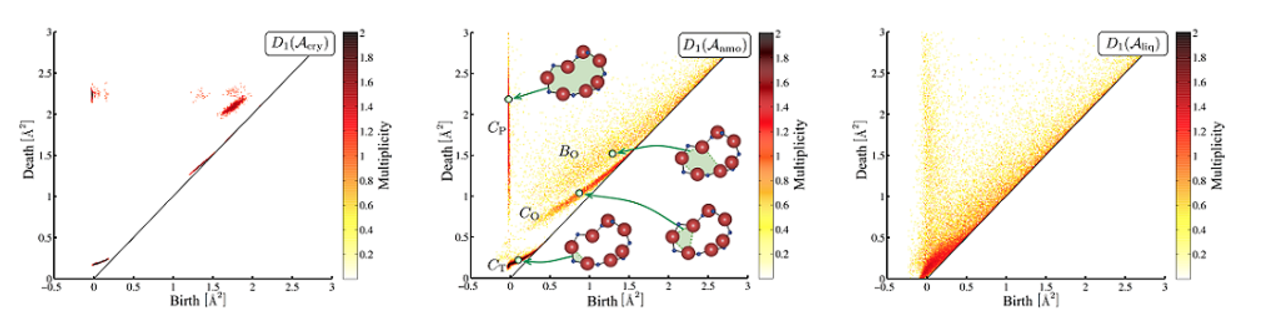
\includegraphics[height=2cm]{persistence_and_materials}
\caption{$Si02$ in different states has different P.H. Credit: Hiraoka}
\end{figure}
\end{center}
\begin{minipage}{.43\textwidth}
\begin{figure}
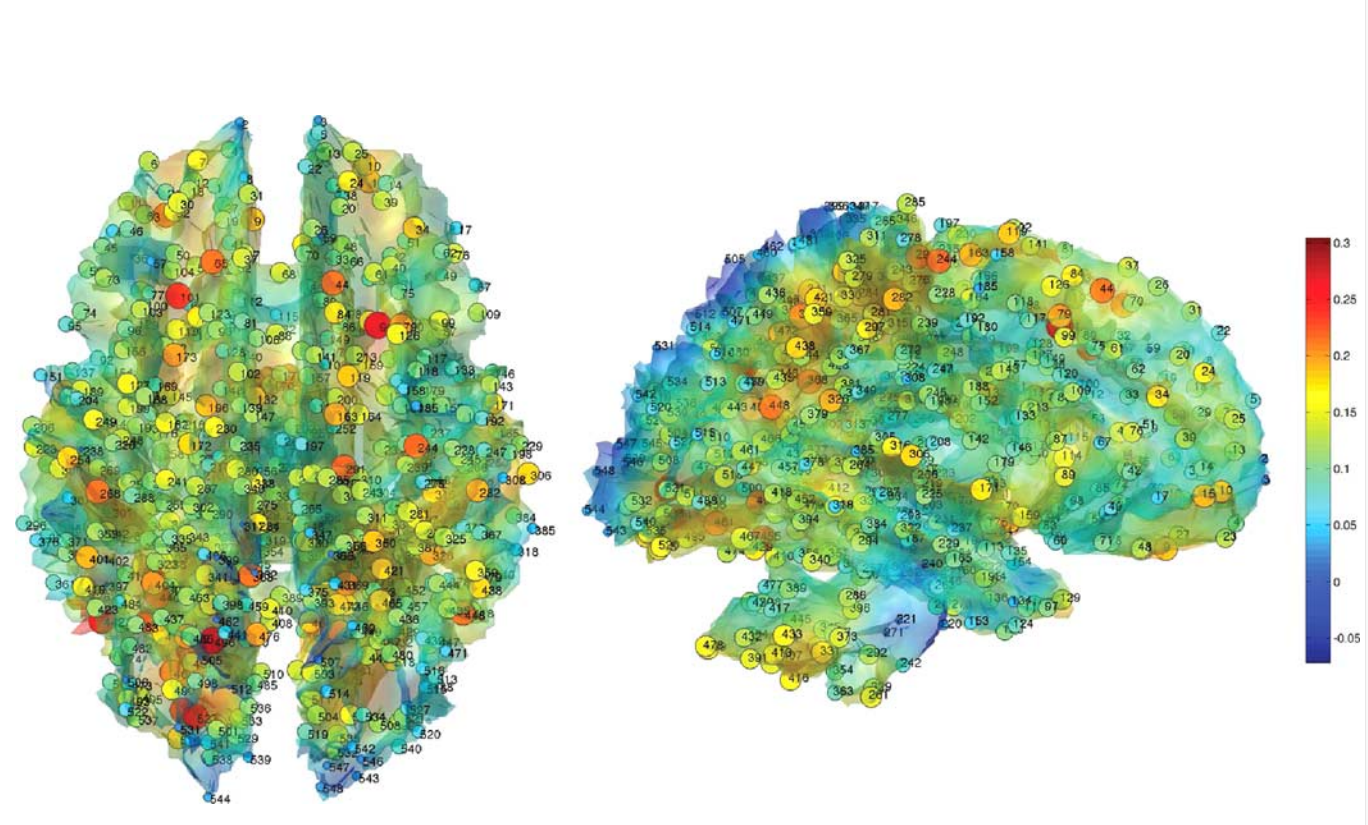
\includegraphics[height=2cm]{complex_on_brains}
\caption{Neuroscience. Credit: Chung}
\end{figure}
\end{minipage}
\begin{minipage}{.43\textwidth}
\hfill
\begin{figure}
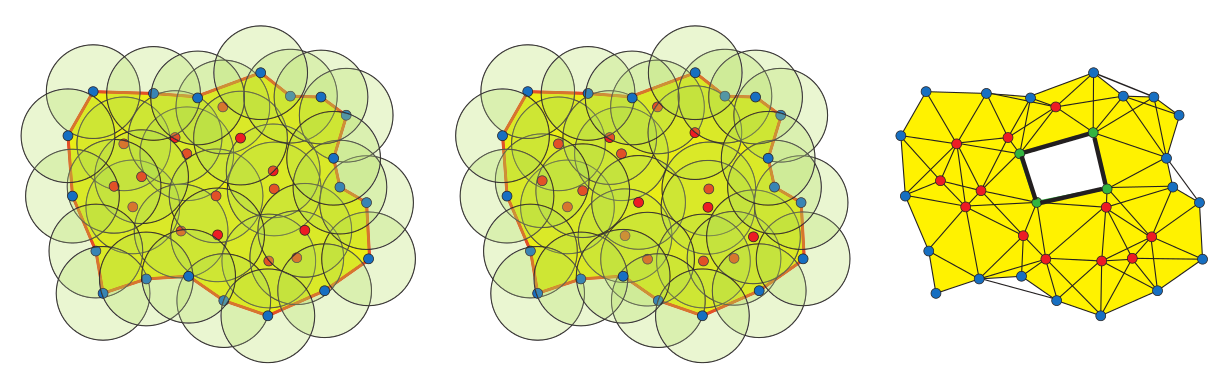
\includegraphics[height=2cm]{sensors}
\caption{Sensor Networks}
\end{figure}
\vfill
\vspace{.5cm}
\end{minipage}
\end{frame}
%
\begin{frame}
\frametitle{A model space}
\begin{minipage}{.46\columnwidth}
     For a dataset $X$ we study the topology of the \emph{union of balls} 
     \[ M_{\epsilon} = \bigcup_{x \in X} B_{\epsilon}(x) \]
     \only<4->{\textbf{Two Issues:}}
     \setlength{\itemindent}{-3em}
     \begin{description}[\itemindent=0pt]
     \item<4->[\textbf{Scale:}] No natural choice of $\epsilon$! 
     \item<5->[\textbf{Conception:}] How to encode $M_\epsilon$ on computer?
    \end{description}
    \only<6->{\textbf{Answer:} Topology}
    \end{minipage}     
\begin{minipage}{0.55\columnwidth}
\hspace{1cm}
\begin{tikzpicture}[scale=.5]
\only<1>{    \node[draw=none, fill=white] at (0, -5.5) {$r = 0$};}
\only<2-4>{    \node[draw=none, fill=white] at (0, -5.5) {$r = .8$};}
\only<5>{    \node[draw=none, fill=white] at (0, -5.5) {$r = .2$};}
\only<6>{    \node[draw=none, fill=white] at (0, -7.5) {$r = \infty$};}
\only<7>{    \node[draw=none, fill=white] at (0, -7.5) {$r = .6$};}
    \foreach[count=\p] \x / \y in \data {
\only<2-4>{	\begin{pgfonlayer}{ball}
        \fill[gray!50,radius= .8 cm] (\x,\y) circle{};
        \end{pgfonlayer}{ball}
        }
      \only<5>{	\begin{pgfonlayer}{ball}
        \fill[gray!50,radius= .2 cm] (\x,\y) circle{};
        \end{pgfonlayer}{ball}
        }
        \only<6>{	\begin{pgfonlayer}{ball}
        \fill[gray!50,radius= 2.4 cm] (\x,\y) circle{};
        \end{pgfonlayer}{ball}
        }
        \only<7>{	\begin{pgfonlayer}{ball}
        \fill[gray!50,radius= .6 cm] (\x,\y) circle{};
        \end{pgfonlayer}{ball}
        }
	\node[draw, circle, scale=.25, fill=white](\p) at (\x, \y) {};
    } 
\end{tikzpicture}
\end{minipage}
\end{frame}

\begin{frame}[fragile]
\frametitle{Simplicial Complexes}
\begin{figure}
\centering
  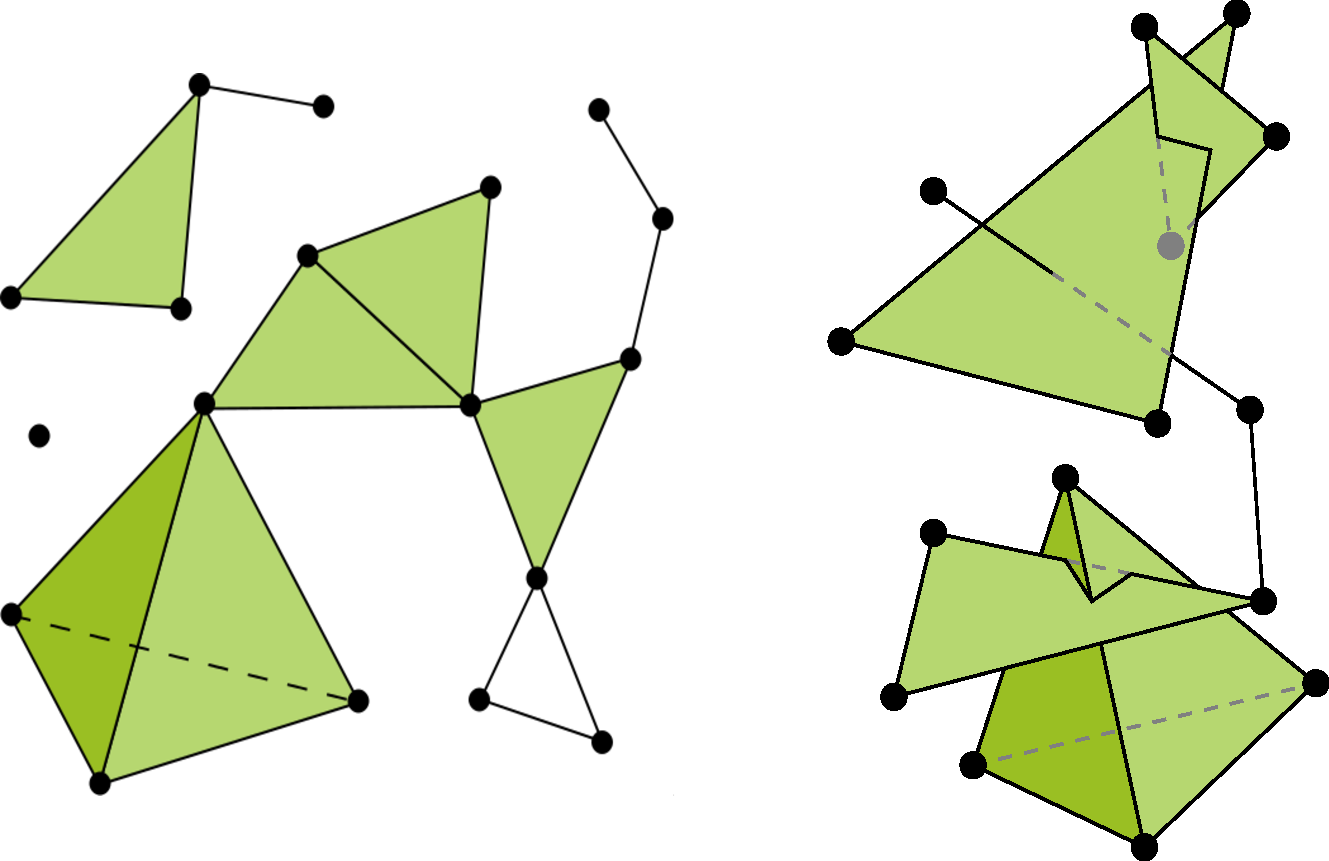
\includegraphics[width=.6\textwidth]{simplicial}
 \caption{(left) an example \phantom{2000}  (right) a non example}
\end{figure}
For a vertex set $V$ a simplicial complex $K \subseteq 2^V$ satisfying:
\begin{enumerate}
\item $\{ v \} \in K$ for each $v \in V$
\item if $\tau \subseteq \sigma \in K$  then $\tau \in K$. 
\item if $\sigma$ is a $k$-simplex if $\card{\sigma} = k+1$ 
\end{enumerate}
\end{frame}

\begin{frame}{Simplicial Complexes}
\centering
\begin{minipage}{0.45\columnwidth}%
\begin{tikzpicture}[scale=.5]
	\node[draw=none, fill=white] at (0, -5.5) {$\check{C}_{.6}$};
    \foreach[count=\p] \x / \y in \data {
	\begin{pgfonlayer}{ball}
        \fill[gray!50,radius= .6 cm] (\x,\y) circle{};
        \end{pgfonlayer}{ball}
	\node[draw, circle, scale=.25, fill=white](\p) at (\x, \y) {};
    } 

\only<3->{
\begin{pgfonlayer}{edge} 
\draw (1) -- (6); 
\draw (1) -- (12); 
\draw (1) -- (19); 
\draw (1) -- (23); 
\draw (1) -- (26); 
\draw (1) -- (48); 
\draw (1) -- (50); 
\draw (1) -- (57); 
\draw (1) -- (68); 
\draw (1) -- (71); 
\draw (1) -- (96); 
\draw (1) -- (98); 
\draw (2) -- (8); 
\draw (2) -- (35); 
\draw (2) -- (47); 
\draw (2) -- (58); 
\draw (2) -- (64); 
\draw (2) -- (89); 
\draw (2) -- (97); 
\draw (3) -- (29); 
\draw (3) -- (39); 
\draw (3) -- (40); 
\draw (3) -- (51); 
\draw (3) -- (65); 
\draw (3) -- (73); 
\draw (3) -- (81); 
\draw (3) -- (91); 
\draw (3) -- (94); 
\draw (4) -- (59); 
\draw (4) -- (70); 
\draw (4) -- (85); 
\draw (4) -- (86); 
\draw (4) -- (88); 
\draw (4) -- (99); 
\draw (4) -- (102); 
\draw (5) -- (24); 
\draw (5) -- (54); 
\draw (5) -- (58); 
\draw (5) -- (63); 
\draw (5) -- (64); 
\draw (5) -- (100); 
\draw (6) -- (19); 
\draw (6) -- (26); 
\draw (6) -- (48); 
\draw (6) -- (57); 
\draw (6) -- (68); 
\draw (6) -- (71); 
\draw (6) -- (98); 
\draw (7) -- (15); 
\draw (7) -- (21); 
\draw (7) -- (39); 
\draw (7) -- (53); 
\draw (7) -- (81); 
\draw (8) -- (18); 
\draw (8) -- (24); 
\draw (8) -- (35); 
\draw (8) -- (54); 
\draw (8) -- (55); 
\draw (8) -- (63); 
\draw (8) -- (64); 
\draw (8) -- (89); 
\draw (9) -- (12); 
\draw (9) -- (23); 
\draw (9) -- (26); 
\draw (9) -- (28); 
\draw (9) -- (32); 
\draw (9) -- (50); 
\draw (9) -- (56); 
\draw (9) -- (67); 
\draw (9) -- (96); 
\draw (10) -- (29); 
\draw (10) -- (40); 
\draw (10) -- (49); 
\draw (10) -- (52); 
\draw (10) -- (65); 
\draw (10) -- (69); 
\draw (10) -- (77); 
\draw (10) -- (78); 
\draw (10) -- (80); 
\draw (10) -- (83); 
\draw (11) -- (13); 
\draw (11) -- (20); 
\draw (11) -- (33); 
\draw (11) -- (41); 
\draw (11) -- (44); 
\draw (11) -- (45); 
\draw (11) -- (46); 
\draw (11) -- (72); 
\draw (11) -- (90); 
\draw (11) -- (93); 
\draw (11) -- (95); 
\draw (12) -- (23); 
\draw (12) -- (25); 
\draw (12) -- (26); 
\draw (12) -- (28); 
\draw (12) -- (32); 
\draw (12) -- (50); 
\draw (12) -- (67); 
\draw (12) -- (68); 
\draw (12) -- (87); 
\draw (12) -- (96); 
\draw (12) -- (98); 
\draw (13) -- (20); 
\draw (13) -- (44); 
\draw (13) -- (61); 
\draw (13) -- (72); 
\draw (13) -- (82); 
\draw (13) -- (90); 
\draw (13) -- (95); 
\draw (14) -- (30); 
\draw (14) -- (31); 
\draw (14) -- (34); 
\draw (14) -- (43); 
\draw (14) -- (55); 
\draw (14) -- (60); 
\draw (14) -- (75); 
\draw (14) -- (76); 
\draw (14) -- (84); 
\draw (14) -- (92); 
\draw (15) -- (21); 
\draw (15) -- (39); 
\draw (15) -- (51); 
\draw (15) -- (53); 
\draw (15) -- (65); 
\draw (15) -- (73); 
\draw (15) -- (81); 
\draw (16) -- (17); 
\draw (16) -- (19); 
\draw (16) -- (38); 
\draw (16) -- (57); 
\draw (16) -- (62); 
\draw (16) -- (79); 
\draw (17) -- (22); 
\draw (17) -- (38); 
\draw (17) -- (57); 
\draw (17) -- (62); 
\draw (17) -- (74); 
\draw (17) -- (79); 
\draw (18) -- (35); 
\draw (18) -- (54); 
\draw (18) -- (55); 
\draw (18) -- (63); 
\draw (18) -- (64); 
\draw (18) -- (76); 
\draw (18) -- (89); 
\draw (19) -- (48); 
\draw (19) -- (57); 
\draw (19) -- (71); 
\draw (19) -- (79); 
\draw (20) -- (41); 
\draw (20) -- (44); 
\draw (20) -- (45); 
\draw (20) -- (46); 
\draw (20) -- (72); 
\draw (20) -- (82); 
\draw (20) -- (90); 
\draw (20) -- (93); 
\draw (20) -- (95); 
\draw (21) -- (39); 
\draw (21) -- (53); 
\draw (21) -- (81); 
\draw (21) -- (91); 
\draw (21) -- (94); 
\draw (21) -- (100); 
\draw (22) -- (70); 
\draw (22) -- (74); 
\draw (22) -- (85); 
\draw (22) -- (88); 
\draw (22) -- (99); 
\draw (23) -- (26); 
\draw (23) -- (28); 
\draw (23) -- (32); 
\draw (23) -- (50); 
\draw (23) -- (56); 
\draw (23) -- (67); 
\draw (23) -- (68); 
\draw (23) -- (87); 
\draw (23) -- (96); 
\draw (23) -- (98); 
\draw (24) -- (54); 
\draw (24) -- (58); 
\draw (24) -- (63); 
\draw (24) -- (64); 
\draw (25) -- (28); 
\draw (25) -- (32); 
\draw (25) -- (66); 
\draw (25) -- (67); 
\draw (25) -- (68); 
\draw (25) -- (87); 
\draw (25) -- (96); 
\draw (25) -- (98); 
\draw (26) -- (32); 
\draw (26) -- (50); 
\draw (26) -- (67); 
\draw (26) -- (68); 
\draw (26) -- (96); 
\draw (26) -- (98); 
\draw (27) -- (36); 
\draw (27) -- (37); 
\draw (27) -- (56); 
\draw (27) -- (101); 
\draw (28) -- (32); 
\draw (28) -- (37); 
\draw (28) -- (56); 
\draw (28) -- (66); 
\draw (28) -- (67); 
\draw (28) -- (87); 
\draw (28) -- (96); 
\draw (28) -- (101); 
\draw (29) -- (40); 
\draw (29) -- (51); 
\draw (29) -- (52); 
\draw (29) -- (65); 
\draw (29) -- (73); 
\draw (29) -- (77); 
\draw (29) -- (78); 
\draw (29) -- (80); 
\draw (29) -- (83); 
\draw (30) -- (31); 
\draw (30) -- (34); 
\draw (30) -- (43); 
\draw (30) -- (55); 
\draw (30) -- (60); 
\draw (30) -- (75); 
\draw (30) -- (76); 
\draw (30) -- (84); 
\draw (30) -- (92); 
\draw (31) -- (43); 
\draw (31) -- (55); 
\draw (31) -- (60); 
\draw (31) -- (75); 
\draw (31) -- (76); 
\draw (31) -- (84); 
\draw (31) -- (92); 
\draw (32) -- (50); 
\draw (32) -- (56); 
\draw (32) -- (67); 
\draw (32) -- (68); 
\draw (32) -- (87); 
\draw (32) -- (96); 
\draw (32) -- (98); 
\draw (33) -- (41); 
\draw (33) -- (46); 
\draw (33) -- (86); 
\draw (33) -- (93); 
\draw (34) -- (36); 
\draw (34) -- (37); 
\draw (34) -- (43); 
\draw (34) -- (60); 
\draw (34) -- (66); 
\draw (34) -- (75); 
\draw (34) -- (84); 
\draw (34) -- (92); 
\draw (35) -- (47); 
\draw (35) -- (55); 
\draw (35) -- (64); 
\draw (35) -- (76); 
\draw (35) -- (89); 
\draw (36) -- (37); 
\draw (36) -- (66); 
\draw (36) -- (84); 
\draw (36) -- (101); 
\draw (37) -- (56); 
\draw (37) -- (66); 
\draw (37) -- (101); 
\draw (38) -- (62); 
\draw (38) -- (74); 
\draw (39) -- (73); 
\draw (39) -- (81); 
\draw (39) -- (91); 
\draw (39) -- (94); 
\draw (40) -- (42); 
\draw (40) -- (49); 
\draw (40) -- (52); 
\draw (40) -- (73); 
\draw (40) -- (77); 
\draw (40) -- (78); 
\draw (40) -- (80); 
\draw (40) -- (83); 
\draw (41) -- (44); 
\draw (41) -- (45); 
\draw (41) -- (46); 
\draw (41) -- (72); 
\draw (41) -- (90); 
\draw (41) -- (93); 
\draw (41) -- (95); 
\draw (41) -- (102); 
\draw (42) -- (44); 
\draw (42) -- (49); 
\draw (42) -- (61); 
\draw (42) -- (69); 
\draw (42) -- (77); 
\draw (42) -- (78); 
\draw (42) -- (80); 
\draw (42) -- (82); 
\draw (42) -- (90); 
\draw (42) -- (95); 
\draw (43) -- (60); 
\draw (43) -- (75); 
\draw (43) -- (76); 
\draw (43) -- (84); 
\draw (43) -- (92); 
\draw (44) -- (45); 
\draw (44) -- (46); 
\draw (44) -- (49); 
\draw (44) -- (72); 
\draw (44) -- (82); 
\draw (44) -- (90); 
\draw (44) -- (93); 
\draw (44) -- (95); 
\draw (45) -- (46); 
\draw (45) -- (72); 
\draw (45) -- (82); 
\draw (45) -- (90); 
\draw (45) -- (93); 
\draw (45) -- (95); 
\draw (45) -- (102); 
\draw (46) -- (72); 
\draw (46) -- (90); 
\draw (46) -- (93); 
\draw (46) -- (95); 
\draw (46) -- (102); 
\draw (47) -- (55); 
\draw (47) -- (60); 
\draw (47) -- (89); 
\draw (48) -- (57); 
\draw (48) -- (68); 
\draw (48) -- (71); 
\draw (48) -- (79); 
\draw (48) -- (96); 
\draw (48) -- (98); 
\draw (49) -- (61); 
\draw (49) -- (69); 
\draw (49) -- (77); 
\draw (49) -- (78); 
\draw (49) -- (80); 
\draw (49) -- (82); 
\draw (49) -- (83); 
\draw (49) -- (90); 
\draw (49) -- (95); 
\draw (50) -- (67); 
\draw (50) -- (68); 
\draw (50) -- (96); 
\draw (50) -- (98); 
\draw (51) -- (52); 
\draw (51) -- (65); 
\draw (51) -- (73); 
\draw (52) -- (65); 
\draw (52) -- (73); 
\draw (52) -- (77); 
\draw (52) -- (78); 
\draw (52) -- (80); 
\draw (52) -- (83); 
\draw (53) -- (81); 
\draw (53) -- (100); 
\draw (54) -- (63); 
\draw (54) -- (64); 
\draw (55) -- (60); 
\draw (55) -- (75); 
\draw (55) -- (76); 
\draw (55) -- (89); 
\draw (55) -- (92); 
\draw (56) -- (67); 
\draw (56) -- (101); 
\draw (57) -- (71); 
\draw (57) -- (79); 
\draw (58) -- (64); 
\draw (58) -- (97); 
\draw (58) -- (100); 
\draw (59) -- (70); 
\draw (59) -- (85); 
\draw (59) -- (86); 
\draw (59) -- (88); 
\draw (59) -- (99); 
\draw (60) -- (75); 
\draw (60) -- (76); 
\draw (60) -- (84); 
\draw (60) -- (92); 
\draw (61) -- (69); 
\draw (61) -- (77); 
\draw (61) -- (78); 
\draw (61) -- (80); 
\draw (61) -- (82); 
\draw (61) -- (90); 
\draw (61) -- (95); 
\draw (62) -- (74); 
\draw (62) -- (79); 
\draw (63) -- (64); 
\draw (64) -- (89); 
\draw (65) -- (73); 
\draw (65) -- (83); 
\draw (66) -- (87); 
\draw (67) -- (68); 
\draw (67) -- (87); 
\draw (67) -- (96); 
\draw (67) -- (98); 
\draw (68) -- (71); 
\draw (68) -- (87); 
\draw (68) -- (96); 
\draw (68) -- (98); 
\draw (69) -- (77); 
\draw (69) -- (78); 
\draw (69) -- (80); 
\draw (69) -- (82); 
\draw (69) -- (83); 
\draw (69) -- (95); 
\draw (70) -- (74); 
\draw (70) -- (85); 
\draw (70) -- (88); 
\draw (70) -- (99); 
\draw (71) -- (79); 
\draw (71) -- (98); 
\draw (72) -- (82); 
\draw (72) -- (90); 
\draw (72) -- (93); 
\draw (72) -- (95); 
\draw (73) -- (81); 
\draw (73) -- (91); 
\draw (73) -- (94); 
\draw (74) -- (85); 
\draw (74) -- (88); 
\draw (75) -- (76); 
\draw (75) -- (84); 
\draw (75) -- (92); 
\draw (76) -- (84); 
\draw (76) -- (89); 
\draw (76) -- (92); 
\draw (77) -- (78); 
\draw (77) -- (80); 
\draw (77) -- (82); 
\draw (77) -- (83); 
\draw (78) -- (80); 
\draw (78) -- (83); 
\draw (80) -- (82); 
\draw (80) -- (83); 
\draw (81) -- (91); 
\draw (81) -- (94); 
\draw (82) -- (90); 
\draw (82) -- (93); 
\draw (82) -- (95); 
\draw (84) -- (92); 
\draw (85) -- (86); 
\draw (85) -- (88); 
\draw (85) -- (99); 
\draw (86) -- (99); 
\draw (87) -- (96); 
\draw (87) -- (98); 
\draw (88) -- (99); 
\draw (89) -- (92); 
\draw (90) -- (93); 
\draw (90) -- (95); 
\draw (91) -- (94); 
\draw (91) -- (97); 
\draw (93) -- (95); 
\draw (93) -- (102); 
\draw (96) -- (98); 
\end{pgfonlayer}{edge} 
}
\only<4->{
\begin{pgfonlayer}{triangle} 
\fill[complex_triangle] (1.center) -- (19.center) -- (6.center) -- cycle; 
\fill[complex_triangle] (1.center) -- (26.center) -- (6.center) -- cycle; 
\fill[complex_triangle] (48.center) -- (1.center) -- (6.center) -- cycle; 
\fill[complex_triangle] (1.center) -- (6.center) -- (57.center) -- cycle; 
\fill[complex_triangle] (1.center) -- (68.center) -- (6.center) -- cycle; 
\fill[complex_triangle] (1.center) -- (6.center) -- (71.center) -- cycle; 
\fill[complex_triangle] (1.center) -- (98.center) -- (6.center) -- cycle; 
\fill[complex_triangle] (1.center) -- (12.center) -- (23.center) -- cycle; 
\fill[complex_triangle] (1.center) -- (26.center) -- (12.center) -- cycle; 
\fill[complex_triangle] (1.center) -- (50.center) -- (12.center) -- cycle; 
\fill[complex_triangle] (68.center) -- (1.center) -- (12.center) -- cycle; 
\fill[complex_triangle] (96.center) -- (1.center) -- (12.center) -- cycle; 
\fill[complex_triangle] (1.center) -- (98.center) -- (12.center) -- cycle; 
\fill[complex_triangle] (48.center) -- (1.center) -- (19.center) -- cycle; 
\fill[complex_triangle] (1.center) -- (19.center) -- (57.center) -- cycle; 
\fill[complex_triangle] (1.center) -- (19.center) -- (71.center) -- cycle; 
\fill[complex_triangle] (1.center) -- (26.center) -- (23.center) -- cycle; 
\fill[complex_triangle] (1.center) -- (50.center) -- (23.center) -- cycle; 
\fill[complex_triangle] (1.center) -- (68.center) -- (23.center) -- cycle; 
\fill[complex_triangle] (96.center) -- (1.center) -- (23.center) -- cycle; 
\fill[complex_triangle] (1.center) -- (98.center) -- (23.center) -- cycle; 
\fill[complex_triangle] (1.center) -- (26.center) -- (50.center) -- cycle; 
\fill[complex_triangle] (1.center) -- (26.center) -- (68.center) -- cycle; 
\fill[complex_triangle] (96.center) -- (1.center) -- (26.center) -- cycle; 
\fill[complex_triangle] (1.center) -- (26.center) -- (98.center) -- cycle; 
\fill[complex_triangle] (48.center) -- (1.center) -- (57.center) -- cycle; 
\fill[complex_triangle] (48.center) -- (1.center) -- (68.center) -- cycle; 
\fill[complex_triangle] (48.center) -- (1.center) -- (71.center) -- cycle; 
\fill[complex_triangle] (48.center) -- (1.center) -- (96.center) -- cycle; 
\fill[complex_triangle] (48.center) -- (1.center) -- (98.center) -- cycle; 
\fill[complex_triangle] (1.center) -- (50.center) -- (68.center) -- cycle; 
\fill[complex_triangle] (96.center) -- (1.center) -- (50.center) -- cycle; 
\fill[complex_triangle] (1.center) -- (50.center) -- (98.center) -- cycle; 
\fill[complex_triangle] (1.center) -- (71.center) -- (57.center) -- cycle; 
\fill[complex_triangle] (1.center) -- (68.center) -- (71.center) -- cycle; 
\fill[complex_triangle] (96.center) -- (1.center) -- (68.center) -- cycle; 
\fill[complex_triangle] (1.center) -- (98.center) -- (68.center) -- cycle; 
\fill[complex_triangle] (1.center) -- (98.center) -- (71.center) -- cycle; 
\fill[complex_triangle] (96.center) -- (1.center) -- (98.center) -- cycle; 
\fill[complex_triangle] (8.center) -- (2.center) -- (35.center) -- cycle; 
\fill[complex_triangle] (8.center) -- (64.center) -- (2.center) -- cycle; 
\fill[complex_triangle] (8.center) -- (89.center) -- (2.center) -- cycle; 
\fill[complex_triangle] (2.center) -- (35.center) -- (47.center) -- cycle; 
\fill[complex_triangle] (64.center) -- (2.center) -- (35.center) -- cycle; 
\fill[complex_triangle] (89.center) -- (2.center) -- (35.center) -- cycle; 
\fill[complex_triangle] (89.center) -- (2.center) -- (47.center) -- cycle; 
\fill[complex_triangle] (64.center) -- (2.center) -- (58.center) -- cycle; 
\fill[complex_triangle] (97.center) -- (2.center) -- (58.center) -- cycle; 
\fill[complex_triangle] (64.center) -- (89.center) -- (2.center) -- cycle; 
\fill[complex_triangle] (40.center) -- (3.center) -- (29.center) -- cycle; 
\fill[complex_triangle] (51.center) -- (3.center) -- (29.center) -- cycle; 
\fill[complex_triangle] (65.center) -- (3.center) -- (29.center) -- cycle; 
\fill[complex_triangle] (73.center) -- (3.center) -- (29.center) -- cycle; 
\fill[complex_triangle] (73.center) -- (3.center) -- (39.center) -- cycle; 
\fill[complex_triangle] (81.center) -- (3.center) -- (39.center) -- cycle; 
\fill[complex_triangle] (91.center) -- (3.center) -- (39.center) -- cycle; 
\fill[complex_triangle] (3.center) -- (94.center) -- (39.center) -- cycle; 
\fill[complex_triangle] (40.center) -- (73.center) -- (3.center) -- cycle; 
\fill[complex_triangle] (51.center) -- (3.center) -- (65.center) -- cycle; 
\fill[complex_triangle] (51.center) -- (3.center) -- (73.center) -- cycle; 
\fill[complex_triangle] (65.center) -- (3.center) -- (73.center) -- cycle; 
\fill[complex_triangle] (73.center) -- (3.center) -- (81.center) -- cycle; 
\fill[complex_triangle] (73.center) -- (91.center) -- (3.center) -- cycle; 
\fill[complex_triangle] (73.center) -- (3.center) -- (94.center) -- cycle; 
\fill[complex_triangle] (81.center) -- (91.center) -- (3.center) -- cycle; 
\fill[complex_triangle] (81.center) -- (3.center) -- (94.center) -- cycle; 
\fill[complex_triangle] (91.center) -- (3.center) -- (94.center) -- cycle; 
\fill[complex_triangle] (59.center) -- (4.center) -- (70.center) -- cycle; 
\fill[complex_triangle] (59.center) -- (4.center) -- (85.center) -- cycle; 
\fill[complex_triangle] (59.center) -- (4.center) -- (86.center) -- cycle; 
\fill[complex_triangle] (88.center) -- (59.center) -- (4.center) -- cycle; 
\fill[complex_triangle] (99.center) -- (59.center) -- (4.center) -- cycle; 
\fill[complex_triangle] (4.center) -- (85.center) -- (70.center) -- cycle; 
\fill[complex_triangle] (88.center) -- (4.center) -- (70.center) -- cycle; 
\fill[complex_triangle] (99.center) -- (4.center) -- (70.center) -- cycle; 
\fill[complex_triangle] (4.center) -- (85.center) -- (86.center) -- cycle; 
\fill[complex_triangle] (88.center) -- (4.center) -- (85.center) -- cycle; 
\fill[complex_triangle] (99.center) -- (4.center) -- (85.center) -- cycle; 
\fill[complex_triangle] (99.center) -- (4.center) -- (86.center) -- cycle; 
\fill[complex_triangle] (88.center) -- (99.center) -- (4.center) -- cycle; 
\fill[complex_triangle] (24.center) -- (5.center) -- (54.center) -- cycle; 
\fill[complex_triangle] (24.center) -- (58.center) -- (5.center) -- cycle; 
\fill[complex_triangle] (24.center) -- (5.center) -- (63.center) -- cycle; 
\fill[complex_triangle] (24.center) -- (64.center) -- (5.center) -- cycle; 
\fill[complex_triangle] (5.center) -- (54.center) -- (63.center) -- cycle; 
\fill[complex_triangle] (64.center) -- (5.center) -- (54.center) -- cycle; 
\fill[complex_triangle] (64.center) -- (58.center) -- (5.center) -- cycle; 
\fill[complex_triangle] (58.center) -- (100.center) -- (5.center) -- cycle; 
\fill[complex_triangle] (64.center) -- (5.center) -- (63.center) -- cycle; 
\fill[complex_triangle] (48.center) -- (19.center) -- (6.center) -- cycle; 
\fill[complex_triangle] (57.center) -- (19.center) -- (6.center) -- cycle; 
\fill[complex_triangle] (19.center) -- (6.center) -- (71.center) -- cycle; 
\fill[complex_triangle] (26.center) -- (68.center) -- (6.center) -- cycle; 
\fill[complex_triangle] (26.center) -- (98.center) -- (6.center) -- cycle; 
\fill[complex_triangle] (48.center) -- (57.center) -- (6.center) -- cycle; 
\fill[complex_triangle] (48.center) -- (68.center) -- (6.center) -- cycle; 
\fill[complex_triangle] (48.center) -- (6.center) -- (71.center) -- cycle; 
\fill[complex_triangle] (48.center) -- (98.center) -- (6.center) -- cycle; 
\fill[complex_triangle] (57.center) -- (6.center) -- (71.center) -- cycle; 
\fill[complex_triangle] (68.center) -- (6.center) -- (71.center) -- cycle; 
\fill[complex_triangle] (98.center) -- (68.center) -- (6.center) -- cycle; 
\fill[complex_triangle] (98.center) -- (6.center) -- (71.center) -- cycle; 
\fill[complex_triangle] (15.center) -- (21.center) -- (7.center) -- cycle; 
\fill[complex_triangle] (39.center) -- (15.center) -- (7.center) -- cycle; 
\fill[complex_triangle] (15.center) -- (53.center) -- (7.center) -- cycle; 
\fill[complex_triangle] (81.center) -- (15.center) -- (7.center) -- cycle; 
\fill[complex_triangle] (39.center) -- (21.center) -- (7.center) -- cycle; 
\fill[complex_triangle] (53.center) -- (21.center) -- (7.center) -- cycle; 
\fill[complex_triangle] (81.center) -- (21.center) -- (7.center) -- cycle; 
\fill[complex_triangle] (81.center) -- (39.center) -- (7.center) -- cycle; 
\fill[complex_triangle] (81.center) -- (53.center) -- (7.center) -- cycle; 
\fill[complex_triangle] (8.center) -- (18.center) -- (35.center) -- cycle; 
\fill[complex_triangle] (8.center) -- (18.center) -- (54.center) -- cycle; 
\fill[complex_triangle] (8.center) -- (18.center) -- (55.center) -- cycle; 
\fill[complex_triangle] (8.center) -- (18.center) -- (63.center) -- cycle; 
\fill[complex_triangle] (8.center) -- (64.center) -- (18.center) -- cycle; 
\fill[complex_triangle] (8.center) -- (89.center) -- (18.center) -- cycle; 
\fill[complex_triangle] (8.center) -- (24.center) -- (54.center) -- cycle; 
\fill[complex_triangle] (8.center) -- (24.center) -- (63.center) -- cycle; 
\fill[complex_triangle] (8.center) -- (24.center) -- (64.center) -- cycle; 
\fill[complex_triangle] (8.center) -- (35.center) -- (55.center) -- cycle; 
\fill[complex_triangle] (8.center) -- (64.center) -- (35.center) -- cycle; 
\fill[complex_triangle] (8.center) -- (89.center) -- (35.center) -- cycle; 
\fill[complex_triangle] (8.center) -- (54.center) -- (63.center) -- cycle; 
\fill[complex_triangle] (8.center) -- (64.center) -- (54.center) -- cycle; 
\fill[complex_triangle] (8.center) -- (89.center) -- (55.center) -- cycle; 
\fill[complex_triangle] (8.center) -- (64.center) -- (63.center) -- cycle; 
\fill[complex_triangle] (8.center) -- (64.center) -- (89.center) -- cycle; 
\fill[complex_triangle] (9.center) -- (12.center) -- (23.center) -- cycle; 
\fill[complex_triangle] (9.center) -- (26.center) -- (12.center) -- cycle; 
\fill[complex_triangle] (9.center) -- (12.center) -- (28.center) -- cycle; 
\fill[complex_triangle] (32.center) -- (9.center) -- (12.center) -- cycle; 
\fill[complex_triangle] (9.center) -- (50.center) -- (12.center) -- cycle; 
\fill[complex_triangle] (9.center) -- (67.center) -- (12.center) -- cycle; 
\fill[complex_triangle] (96.center) -- (9.center) -- (12.center) -- cycle; 
\fill[complex_triangle] (9.center) -- (26.center) -- (23.center) -- cycle; 
\fill[complex_triangle] (9.center) -- (28.center) -- (23.center) -- cycle; 
\fill[complex_triangle] (32.center) -- (9.center) -- (23.center) -- cycle; 
\fill[complex_triangle] (9.center) -- (50.center) -- (23.center) -- cycle; 
\fill[complex_triangle] (56.center) -- (9.center) -- (23.center) -- cycle; 
\fill[complex_triangle] (9.center) -- (67.center) -- (23.center) -- cycle; 
\fill[complex_triangle] (96.center) -- (9.center) -- (23.center) -- cycle; 
\fill[complex_triangle] (32.center) -- (9.center) -- (26.center) -- cycle; 
\fill[complex_triangle] (9.center) -- (26.center) -- (50.center) -- cycle; 
\fill[complex_triangle] (9.center) -- (26.center) -- (67.center) -- cycle; 
\fill[complex_triangle] (96.center) -- (9.center) -- (26.center) -- cycle; 
\fill[complex_triangle] (32.center) -- (9.center) -- (28.center) -- cycle; 
\fill[complex_triangle] (56.center) -- (9.center) -- (28.center) -- cycle; 
\fill[complex_triangle] (9.center) -- (67.center) -- (28.center) -- cycle; 
\fill[complex_triangle] (96.center) -- (9.center) -- (28.center) -- cycle; 
\fill[complex_triangle] (32.center) -- (9.center) -- (50.center) -- cycle; 
\fill[complex_triangle] (32.center) -- (9.center) -- (56.center) -- cycle; 
\fill[complex_triangle] (32.center) -- (9.center) -- (67.center) -- cycle; 
\fill[complex_triangle] (32.center) -- (9.center) -- (96.center) -- cycle; 
\fill[complex_triangle] (9.center) -- (50.center) -- (67.center) -- cycle; 
\fill[complex_triangle] (96.center) -- (9.center) -- (50.center) -- cycle; 
\fill[complex_triangle] (56.center) -- (9.center) -- (67.center) -- cycle; 
\fill[complex_triangle] (96.center) -- (9.center) -- (67.center) -- cycle; 
\fill[complex_triangle] (40.center) -- (10.center) -- (29.center) -- cycle; 
\fill[complex_triangle] (10.center) -- (52.center) -- (29.center) -- cycle; 
\fill[complex_triangle] (65.center) -- (10.center) -- (29.center) -- cycle; 
\fill[complex_triangle] (10.center) -- (29.center) -- (77.center) -- cycle; 
\fill[complex_triangle] (10.center) -- (29.center) -- (78.center) -- cycle; 
\fill[complex_triangle] (80.center) -- (10.center) -- (29.center) -- cycle; 
\fill[complex_triangle] (10.center) -- (83.center) -- (29.center) -- cycle; 
\fill[complex_triangle] (40.center) -- (49.center) -- (10.center) -- cycle; 
\fill[complex_triangle] (40.center) -- (10.center) -- (52.center) -- cycle; 
\fill[complex_triangle] (40.center) -- (10.center) -- (77.center) -- cycle; 
\fill[complex_triangle] (40.center) -- (10.center) -- (78.center) -- cycle; 
\fill[complex_triangle] (40.center) -- (80.center) -- (10.center) -- cycle; 
\fill[complex_triangle] (40.center) -- (10.center) -- (83.center) -- cycle; 
\fill[complex_triangle] (49.center) -- (10.center) -- (69.center) -- cycle; 
\fill[complex_triangle] (49.center) -- (10.center) -- (77.center) -- cycle; 
\fill[complex_triangle] (49.center) -- (10.center) -- (78.center) -- cycle; 
\fill[complex_triangle] (80.center) -- (49.center) -- (10.center) -- cycle; 
\fill[complex_triangle] (49.center) -- (10.center) -- (83.center) -- cycle; 
\fill[complex_triangle] (65.center) -- (10.center) -- (52.center) -- cycle; 
\fill[complex_triangle] (10.center) -- (52.center) -- (77.center) -- cycle; 
\fill[complex_triangle] (10.center) -- (52.center) -- (78.center) -- cycle; 
\fill[complex_triangle] (80.center) -- (10.center) -- (52.center) -- cycle; 
\fill[complex_triangle] (10.center) -- (83.center) -- (52.center) -- cycle; 
\fill[complex_triangle] (65.center) -- (10.center) -- (83.center) -- cycle; 
\fill[complex_triangle] (10.center) -- (69.center) -- (77.center) -- cycle; 
\fill[complex_triangle] (10.center) -- (69.center) -- (78.center) -- cycle; 
\fill[complex_triangle] (80.center) -- (10.center) -- (69.center) -- cycle; 
\fill[complex_triangle] (10.center) -- (83.center) -- (69.center) -- cycle; 
\fill[complex_triangle] (10.center) -- (77.center) -- (78.center) -- cycle; 
\fill[complex_triangle] (80.center) -- (10.center) -- (77.center) -- cycle; 
\fill[complex_triangle] (10.center) -- (83.center) -- (77.center) -- cycle; 
\fill[complex_triangle] (80.center) -- (10.center) -- (78.center) -- cycle; 
\fill[complex_triangle] (10.center) -- (83.center) -- (78.center) -- cycle; 
\fill[complex_triangle] (80.center) -- (10.center) -- (83.center) -- cycle; 
\fill[complex_triangle] (11.center) -- (20.center) -- (13.center) -- cycle; 
\fill[complex_triangle] (11.center) -- (44.center) -- (13.center) -- cycle; 
\fill[complex_triangle] (72.center) -- (11.center) -- (13.center) -- cycle; 
\fill[complex_triangle] (90.center) -- (11.center) -- (13.center) -- cycle; 
\fill[complex_triangle] (11.center) -- (13.center) -- (95.center) -- cycle; 
\fill[complex_triangle] (41.center) -- (11.center) -- (20.center) -- cycle; 
\fill[complex_triangle] (44.center) -- (11.center) -- (20.center) -- cycle; 
\fill[complex_triangle] (11.center) -- (20.center) -- (45.center) -- cycle; 
\fill[complex_triangle] (11.center) -- (20.center) -- (46.center) -- cycle; 
\fill[complex_triangle] (72.center) -- (11.center) -- (20.center) -- cycle; 
\fill[complex_triangle] (90.center) -- (11.center) -- (20.center) -- cycle; 
\fill[complex_triangle] (11.center) -- (20.center) -- (93.center) -- cycle; 
\fill[complex_triangle] (11.center) -- (20.center) -- (95.center) -- cycle; 
\fill[complex_triangle] (33.center) -- (11.center) -- (41.center) -- cycle; 
\fill[complex_triangle] (33.center) -- (11.center) -- (46.center) -- cycle; 
\fill[complex_triangle] (33.center) -- (11.center) -- (93.center) -- cycle; 
\fill[complex_triangle] (41.center) -- (11.center) -- (44.center) -- cycle; 
\fill[complex_triangle] (41.center) -- (11.center) -- (45.center) -- cycle; 
\fill[complex_triangle] (41.center) -- (11.center) -- (46.center) -- cycle; 
\fill[complex_triangle] (72.center) -- (41.center) -- (11.center) -- cycle; 
\fill[complex_triangle] (41.center) -- (90.center) -- (11.center) -- cycle; 
\fill[complex_triangle] (41.center) -- (11.center) -- (93.center) -- cycle; 
\fill[complex_triangle] (41.center) -- (11.center) -- (95.center) -- cycle; 
\fill[complex_triangle] (11.center) -- (44.center) -- (45.center) -- cycle; 
\fill[complex_triangle] (11.center) -- (44.center) -- (46.center) -- cycle; 
\fill[complex_triangle] (72.center) -- (11.center) -- (44.center) -- cycle; 
\fill[complex_triangle] (90.center) -- (11.center) -- (44.center) -- cycle; 
\fill[complex_triangle] (11.center) -- (44.center) -- (93.center) -- cycle; 
\fill[complex_triangle] (11.center) -- (44.center) -- (95.center) -- cycle; 
\fill[complex_triangle] (11.center) -- (45.center) -- (46.center) -- cycle; 
\fill[complex_triangle] (72.center) -- (11.center) -- (45.center) -- cycle; 
\fill[complex_triangle] (90.center) -- (11.center) -- (45.center) -- cycle; 
\fill[complex_triangle] (11.center) -- (45.center) -- (93.center) -- cycle; 
\fill[complex_triangle] (11.center) -- (45.center) -- (95.center) -- cycle; 
\fill[complex_triangle] (72.center) -- (11.center) -- (46.center) -- cycle; 
\fill[complex_triangle] (90.center) -- (11.center) -- (46.center) -- cycle; 
\fill[complex_triangle] (11.center) -- (93.center) -- (46.center) -- cycle; 
\fill[complex_triangle] (11.center) -- (46.center) -- (95.center) -- cycle; 
\fill[complex_triangle] (72.center) -- (90.center) -- (11.center) -- cycle; 
\fill[complex_triangle] (72.center) -- (11.center) -- (93.center) -- cycle; 
\fill[complex_triangle] (72.center) -- (11.center) -- (95.center) -- cycle; 
\fill[complex_triangle] (90.center) -- (11.center) -- (93.center) -- cycle; 
\fill[complex_triangle] (90.center) -- (11.center) -- (95.center) -- cycle; 
\fill[complex_triangle] (11.center) -- (93.center) -- (95.center) -- cycle; 
\fill[complex_triangle] (26.center) -- (12.center) -- (23.center) -- cycle; 
\fill[complex_triangle] (28.center) -- (12.center) -- (23.center) -- cycle; 
\fill[complex_triangle] (32.center) -- (12.center) -- (23.center) -- cycle; 
\fill[complex_triangle] (50.center) -- (12.center) -- (23.center) -- cycle; 
\fill[complex_triangle] (67.center) -- (12.center) -- (23.center) -- cycle; 
\fill[complex_triangle] (68.center) -- (12.center) -- (23.center) -- cycle; 
\fill[complex_triangle] (87.center) -- (12.center) -- (23.center) -- cycle; 
\fill[complex_triangle] (96.center) -- (12.center) -- (23.center) -- cycle; 
\fill[complex_triangle] (98.center) -- (12.center) -- (23.center) -- cycle; 
\fill[complex_triangle] (25.center) -- (12.center) -- (28.center) -- cycle; 
\fill[complex_triangle] (32.center) -- (25.center) -- (12.center) -- cycle; 
\fill[complex_triangle] (25.center) -- (67.center) -- (12.center) -- cycle; 
\fill[complex_triangle] (68.center) -- (25.center) -- (12.center) -- cycle; 
\fill[complex_triangle] (25.center) -- (12.center) -- (87.center) -- cycle; 
\fill[complex_triangle] (96.center) -- (25.center) -- (12.center) -- cycle; 
\fill[complex_triangle] (25.center) -- (98.center) -- (12.center) -- cycle; 
\fill[complex_triangle] (32.center) -- (26.center) -- (12.center) -- cycle; 
\fill[complex_triangle] (26.center) -- (12.center) -- (50.center) -- cycle; 
\fill[complex_triangle] (26.center) -- (67.center) -- (12.center) -- cycle; 
\fill[complex_triangle] (68.center) -- (26.center) -- (12.center) -- cycle; 
\fill[complex_triangle] (96.center) -- (26.center) -- (12.center) -- cycle; 
\fill[complex_triangle] (26.center) -- (12.center) -- (98.center) -- cycle; 
\fill[complex_triangle] (32.center) -- (28.center) -- (12.center) -- cycle; 
\fill[complex_triangle] (28.center) -- (67.center) -- (12.center) -- cycle; 
\fill[complex_triangle] (28.center) -- (12.center) -- (87.center) -- cycle; 
\fill[complex_triangle] (96.center) -- (28.center) -- (12.center) -- cycle; 
\fill[complex_triangle] (32.center) -- (50.center) -- (12.center) -- cycle; 
\fill[complex_triangle] (32.center) -- (67.center) -- (12.center) -- cycle; 
\fill[complex_triangle] (32.center) -- (68.center) -- (12.center) -- cycle; 
\fill[complex_triangle] (32.center) -- (12.center) -- (87.center) -- cycle; 
\fill[complex_triangle] (32.center) -- (96.center) -- (12.center) -- cycle; 
\fill[complex_triangle] (32.center) -- (98.center) -- (12.center) -- cycle; 
\fill[complex_triangle] (50.center) -- (67.center) -- (12.center) -- cycle; 
\fill[complex_triangle] (68.center) -- (50.center) -- (12.center) -- cycle; 
\fill[complex_triangle] (96.center) -- (50.center) -- (12.center) -- cycle; 
\fill[complex_triangle] (50.center) -- (12.center) -- (98.center) -- cycle; 
\fill[complex_triangle] (68.center) -- (67.center) -- (12.center) -- cycle; 
\fill[complex_triangle] (67.center) -- (12.center) -- (87.center) -- cycle; 
\fill[complex_triangle] (96.center) -- (67.center) -- (12.center) -- cycle; 
\fill[complex_triangle] (98.center) -- (67.center) -- (12.center) -- cycle; 
\fill[complex_triangle] (68.center) -- (12.center) -- (87.center) -- cycle; 
\fill[complex_triangle] (96.center) -- (68.center) -- (12.center) -- cycle; 
\fill[complex_triangle] (68.center) -- (98.center) -- (12.center) -- cycle; 
\fill[complex_triangle] (96.center) -- (12.center) -- (87.center) -- cycle; 
\fill[complex_triangle] (98.center) -- (12.center) -- (87.center) -- cycle; 
\fill[complex_triangle] (96.center) -- (98.center) -- (12.center) -- cycle; 
\fill[complex_triangle] (44.center) -- (20.center) -- (13.center) -- cycle; 
\fill[complex_triangle] (72.center) -- (20.center) -- (13.center) -- cycle; 
\fill[complex_triangle] (82.center) -- (20.center) -- (13.center) -- cycle; 
\fill[complex_triangle] (90.center) -- (20.center) -- (13.center) -- cycle; 
\fill[complex_triangle] (20.center) -- (13.center) -- (95.center) -- cycle; 
\fill[complex_triangle] (72.center) -- (44.center) -- (13.center) -- cycle; 
\fill[complex_triangle] (82.center) -- (44.center) -- (13.center) -- cycle; 
\fill[complex_triangle] (90.center) -- (44.center) -- (13.center) -- cycle; 
\fill[complex_triangle] (44.center) -- (13.center) -- (95.center) -- cycle; 
\fill[complex_triangle] (82.center) -- (13.center) -- (61.center) -- cycle; 
\fill[complex_triangle] (90.center) -- (13.center) -- (61.center) -- cycle; 
\fill[complex_triangle] (95.center) -- (13.center) -- (61.center) -- cycle; 
\fill[complex_triangle] (72.center) -- (82.center) -- (13.center) -- cycle; 
\fill[complex_triangle] (72.center) -- (90.center) -- (13.center) -- cycle; 
\fill[complex_triangle] (72.center) -- (13.center) -- (95.center) -- cycle; 
\fill[complex_triangle] (82.center) -- (90.center) -- (13.center) -- cycle; 
\fill[complex_triangle] (82.center) -- (13.center) -- (95.center) -- cycle; 
\fill[complex_triangle] (90.center) -- (13.center) -- (95.center) -- cycle; 
\fill[complex_triangle] (30.center) -- (14.center) -- (31.center) -- cycle; 
\fill[complex_triangle] (34.center) -- (30.center) -- (14.center) -- cycle; 
\fill[complex_triangle] (43.center) -- (30.center) -- (14.center) -- cycle; 
\fill[complex_triangle] (30.center) -- (14.center) -- (55.center) -- cycle; 
\fill[complex_triangle] (60.center) -- (30.center) -- (14.center) -- cycle; 
\fill[complex_triangle] (75.center) -- (30.center) -- (14.center) -- cycle; 
\fill[complex_triangle] (76.center) -- (30.center) -- (14.center) -- cycle; 
\fill[complex_triangle] (84.center) -- (30.center) -- (14.center) -- cycle; 
\fill[complex_triangle] (92.center) -- (30.center) -- (14.center) -- cycle; 
\fill[complex_triangle] (43.center) -- (14.center) -- (31.center) -- cycle; 
\fill[complex_triangle] (55.center) -- (14.center) -- (31.center) -- cycle; 
\fill[complex_triangle] (60.center) -- (14.center) -- (31.center) -- cycle; 
\fill[complex_triangle] (75.center) -- (14.center) -- (31.center) -- cycle; 
\fill[complex_triangle] (76.center) -- (14.center) -- (31.center) -- cycle; 
\fill[complex_triangle] (84.center) -- (14.center) -- (31.center) -- cycle; 
\fill[complex_triangle] (92.center) -- (14.center) -- (31.center) -- cycle; 
\fill[complex_triangle] (34.center) -- (43.center) -- (14.center) -- cycle; 
\fill[complex_triangle] (34.center) -- (60.center) -- (14.center) -- cycle; 
\fill[complex_triangle] (34.center) -- (75.center) -- (14.center) -- cycle; 
\fill[complex_triangle] (34.center) -- (84.center) -- (14.center) -- cycle; 
\fill[complex_triangle] (34.center) -- (92.center) -- (14.center) -- cycle; 
\fill[complex_triangle] (43.center) -- (60.center) -- (14.center) -- cycle; 
\fill[complex_triangle] (75.center) -- (43.center) -- (14.center) -- cycle; 
\fill[complex_triangle] (43.center) -- (76.center) -- (14.center) -- cycle; 
\fill[complex_triangle] (43.center) -- (84.center) -- (14.center) -- cycle; 
\fill[complex_triangle] (43.center) -- (92.center) -- (14.center) -- cycle; 
\fill[complex_triangle] (60.center) -- (14.center) -- (55.center) -- cycle; 
\fill[complex_triangle] (75.center) -- (14.center) -- (55.center) -- cycle; 
\fill[complex_triangle] (76.center) -- (14.center) -- (55.center) -- cycle; 
\fill[complex_triangle] (92.center) -- (14.center) -- (55.center) -- cycle; 
\fill[complex_triangle] (75.center) -- (60.center) -- (14.center) -- cycle; 
\fill[complex_triangle] (76.center) -- (60.center) -- (14.center) -- cycle; 
\fill[complex_triangle] (84.center) -- (60.center) -- (14.center) -- cycle; 
\fill[complex_triangle] (92.center) -- (60.center) -- (14.center) -- cycle; 
\fill[complex_triangle] (75.center) -- (76.center) -- (14.center) -- cycle; 
\fill[complex_triangle] (75.center) -- (84.center) -- (14.center) -- cycle; 
\fill[complex_triangle] (75.center) -- (92.center) -- (14.center) -- cycle; 
\fill[complex_triangle] (84.center) -- (76.center) -- (14.center) -- cycle; 
\fill[complex_triangle] (92.center) -- (76.center) -- (14.center) -- cycle; 
\fill[complex_triangle] (92.center) -- (84.center) -- (14.center) -- cycle; 
\fill[complex_triangle] (39.center) -- (21.center) -- (15.center) -- cycle; 
\fill[complex_triangle] (53.center) -- (21.center) -- (15.center) -- cycle; 
\fill[complex_triangle] (81.center) -- (21.center) -- (15.center) -- cycle; 
\fill[complex_triangle] (73.center) -- (39.center) -- (15.center) -- cycle; 
\fill[complex_triangle] (81.center) -- (39.center) -- (15.center) -- cycle; 
\fill[complex_triangle] (65.center) -- (51.center) -- (15.center) -- cycle; 
\fill[complex_triangle] (73.center) -- (51.center) -- (15.center) -- cycle; 
\fill[complex_triangle] (81.center) -- (53.center) -- (15.center) -- cycle; 
\fill[complex_triangle] (65.center) -- (73.center) -- (15.center) -- cycle; 
\fill[complex_triangle] (73.center) -- (81.center) -- (15.center) -- cycle; 
\fill[complex_triangle] (16.center) -- (17.center) -- (38.center) -- cycle; 
\fill[complex_triangle] (16.center) -- (17.center) -- (57.center) -- cycle; 
\fill[complex_triangle] (16.center) -- (17.center) -- (62.center) -- cycle; 
\fill[complex_triangle] (16.center) -- (17.center) -- (79.center) -- cycle; 
\fill[complex_triangle] (16.center) -- (57.center) -- (19.center) -- cycle; 
\fill[complex_triangle] (16.center) -- (19.center) -- (79.center) -- cycle; 
\fill[complex_triangle] (16.center) -- (62.center) -- (38.center) -- cycle; 
\fill[complex_triangle] (16.center) -- (57.center) -- (79.center) -- cycle; 
\fill[complex_triangle] (16.center) -- (62.center) -- (79.center) -- cycle; 
\fill[complex_triangle] (17.center) -- (74.center) -- (22.center) -- cycle; 
\fill[complex_triangle] (17.center) -- (62.center) -- (38.center) -- cycle; 
\fill[complex_triangle] (17.center) -- (74.center) -- (38.center) -- cycle; 
\fill[complex_triangle] (17.center) -- (79.center) -- (57.center) -- cycle; 
\fill[complex_triangle] (17.center) -- (74.center) -- (62.center) -- cycle; 
\fill[complex_triangle] (17.center) -- (62.center) -- (79.center) -- cycle; 
\fill[complex_triangle] (18.center) -- (35.center) -- (55.center) -- cycle; 
\fill[complex_triangle] (64.center) -- (18.center) -- (35.center) -- cycle; 
\fill[complex_triangle] (18.center) -- (35.center) -- (76.center) -- cycle; 
\fill[complex_triangle] (89.center) -- (18.center) -- (35.center) -- cycle; 
\fill[complex_triangle] (18.center) -- (54.center) -- (63.center) -- cycle; 
\fill[complex_triangle] (64.center) -- (18.center) -- (54.center) -- cycle; 
\fill[complex_triangle] (18.center) -- (76.center) -- (55.center) -- cycle; 
\fill[complex_triangle] (89.center) -- (18.center) -- (55.center) -- cycle; 
\fill[complex_triangle] (64.center) -- (18.center) -- (63.center) -- cycle; 
\fill[complex_triangle] (64.center) -- (89.center) -- (18.center) -- cycle; 
\fill[complex_triangle] (89.center) -- (18.center) -- (76.center) -- cycle; 
\fill[complex_triangle] (48.center) -- (57.center) -- (19.center) -- cycle; 
\fill[complex_triangle] (48.center) -- (19.center) -- (71.center) -- cycle; 
\fill[complex_triangle] (48.center) -- (19.center) -- (79.center) -- cycle; 
\fill[complex_triangle] (57.center) -- (19.center) -- (71.center) -- cycle; 
\fill[complex_triangle] (57.center) -- (19.center) -- (79.center) -- cycle; 
\fill[complex_triangle] (79.center) -- (19.center) -- (71.center) -- cycle; 
\fill[complex_triangle] (41.center) -- (20.center) -- (44.center) -- cycle; 
\fill[complex_triangle] (41.center) -- (20.center) -- (45.center) -- cycle; 
\fill[complex_triangle] (41.center) -- (20.center) -- (46.center) -- cycle; 
\fill[complex_triangle] (72.center) -- (41.center) -- (20.center) -- cycle; 
\fill[complex_triangle] (41.center) -- (90.center) -- (20.center) -- cycle; 
\fill[complex_triangle] (41.center) -- (20.center) -- (93.center) -- cycle; 
\fill[complex_triangle] (41.center) -- (20.center) -- (95.center) -- cycle; 
\fill[complex_triangle] (44.center) -- (20.center) -- (45.center) -- cycle; 
\fill[complex_triangle] (44.center) -- (20.center) -- (46.center) -- cycle; 
\fill[complex_triangle] (72.center) -- (44.center) -- (20.center) -- cycle; 
\fill[complex_triangle] (44.center) -- (82.center) -- (20.center) -- cycle; 
\fill[complex_triangle] (44.center) -- (90.center) -- (20.center) -- cycle; 
\fill[complex_triangle] (44.center) -- (20.center) -- (93.center) -- cycle; 
\fill[complex_triangle] (44.center) -- (20.center) -- (95.center) -- cycle; 
\fill[complex_triangle] (20.center) -- (45.center) -- (46.center) -- cycle; 
\fill[complex_triangle] (72.center) -- (20.center) -- (45.center) -- cycle; 
\fill[complex_triangle] (82.center) -- (20.center) -- (45.center) -- cycle; 
\fill[complex_triangle] (90.center) -- (20.center) -- (45.center) -- cycle; 
\fill[complex_triangle] (20.center) -- (45.center) -- (93.center) -- cycle; 
\fill[complex_triangle] (20.center) -- (45.center) -- (95.center) -- cycle; 
\fill[complex_triangle] (72.center) -- (20.center) -- (46.center) -- cycle; 
\fill[complex_triangle] (90.center) -- (20.center) -- (46.center) -- cycle; 
\fill[complex_triangle] (20.center) -- (93.center) -- (46.center) -- cycle; 
\fill[complex_triangle] (20.center) -- (46.center) -- (95.center) -- cycle; 
\fill[complex_triangle] (72.center) -- (82.center) -- (20.center) -- cycle; 
\fill[complex_triangle] (72.center) -- (90.center) -- (20.center) -- cycle; 
\fill[complex_triangle] (72.center) -- (20.center) -- (93.center) -- cycle; 
\fill[complex_triangle] (72.center) -- (20.center) -- (95.center) -- cycle; 
\fill[complex_triangle] (82.center) -- (20.center) -- (90.center) -- cycle; 
\fill[complex_triangle] (82.center) -- (20.center) -- (93.center) -- cycle; 
\fill[complex_triangle] (82.center) -- (20.center) -- (95.center) -- cycle; 
\fill[complex_triangle] (90.center) -- (20.center) -- (93.center) -- cycle; 
\fill[complex_triangle] (90.center) -- (20.center) -- (95.center) -- cycle; 
\fill[complex_triangle] (20.center) -- (93.center) -- (95.center) -- cycle; 
\fill[complex_triangle] (81.center) -- (21.center) -- (39.center) -- cycle; 
\fill[complex_triangle] (91.center) -- (21.center) -- (39.center) -- cycle; 
\fill[complex_triangle] (21.center) -- (94.center) -- (39.center) -- cycle; 
\fill[complex_triangle] (81.center) -- (21.center) -- (53.center) -- cycle; 
\fill[complex_triangle] (100.center) -- (21.center) -- (53.center) -- cycle; 
\fill[complex_triangle] (81.center) -- (91.center) -- (21.center) -- cycle; 
\fill[complex_triangle] (81.center) -- (21.center) -- (94.center) -- cycle; 
\fill[complex_triangle] (91.center) -- (21.center) -- (94.center) -- cycle; 
\fill[complex_triangle] (74.center) -- (70.center) -- (22.center) -- cycle; 
\fill[complex_triangle] (70.center) -- (22.center) -- (85.center) -- cycle; 
\fill[complex_triangle] (88.center) -- (70.center) -- (22.center) -- cycle; 
\fill[complex_triangle] (99.center) -- (70.center) -- (22.center) -- cycle; 
\fill[complex_triangle] (74.center) -- (85.center) -- (22.center) -- cycle; 
\fill[complex_triangle] (88.center) -- (74.center) -- (22.center) -- cycle; 
\fill[complex_triangle] (88.center) -- (85.center) -- (22.center) -- cycle; 
\fill[complex_triangle] (99.center) -- (85.center) -- (22.center) -- cycle; 
\fill[complex_triangle] (88.center) -- (99.center) -- (22.center) -- cycle; 
\fill[complex_triangle] (32.center) -- (26.center) -- (23.center) -- cycle; 
\fill[complex_triangle] (26.center) -- (50.center) -- (23.center) -- cycle; 
\fill[complex_triangle] (26.center) -- (67.center) -- (23.center) -- cycle; 
\fill[complex_triangle] (26.center) -- (68.center) -- (23.center) -- cycle; 
\fill[complex_triangle] (96.center) -- (26.center) -- (23.center) -- cycle; 
\fill[complex_triangle] (26.center) -- (98.center) -- (23.center) -- cycle; 
\fill[complex_triangle] (32.center) -- (28.center) -- (23.center) -- cycle; 
\fill[complex_triangle] (56.center) -- (28.center) -- (23.center) -- cycle; 
\fill[complex_triangle] (67.center) -- (28.center) -- (23.center) -- cycle; 
\fill[complex_triangle] (87.center) -- (28.center) -- (23.center) -- cycle; 
\fill[complex_triangle] (96.center) -- (28.center) -- (23.center) -- cycle; 
\fill[complex_triangle] (32.center) -- (50.center) -- (23.center) -- cycle; 
\fill[complex_triangle] (32.center) -- (56.center) -- (23.center) -- cycle; 
\fill[complex_triangle] (32.center) -- (67.center) -- (23.center) -- cycle; 
\fill[complex_triangle] (32.center) -- (68.center) -- (23.center) -- cycle; 
\fill[complex_triangle] (32.center) -- (87.center) -- (23.center) -- cycle; 
\fill[complex_triangle] (32.center) -- (96.center) -- (23.center) -- cycle; 
\fill[complex_triangle] (32.center) -- (98.center) -- (23.center) -- cycle; 
\fill[complex_triangle] (50.center) -- (67.center) -- (23.center) -- cycle; 
\fill[complex_triangle] (50.center) -- (68.center) -- (23.center) -- cycle; 
\fill[complex_triangle] (96.center) -- (50.center) -- (23.center) -- cycle; 
\fill[complex_triangle] (50.center) -- (98.center) -- (23.center) -- cycle; 
\fill[complex_triangle] (56.center) -- (67.center) -- (23.center) -- cycle; 
\fill[complex_triangle] (67.center) -- (68.center) -- (23.center) -- cycle; 
\fill[complex_triangle] (87.center) -- (67.center) -- (23.center) -- cycle; 
\fill[complex_triangle] (96.center) -- (67.center) -- (23.center) -- cycle; 
\fill[complex_triangle] (98.center) -- (67.center) -- (23.center) -- cycle; 
\fill[complex_triangle] (87.center) -- (68.center) -- (23.center) -- cycle; 
\fill[complex_triangle] (96.center) -- (68.center) -- (23.center) -- cycle; 
\fill[complex_triangle] (98.center) -- (68.center) -- (23.center) -- cycle; 
\fill[complex_triangle] (96.center) -- (87.center) -- (23.center) -- cycle; 
\fill[complex_triangle] (98.center) -- (87.center) -- (23.center) -- cycle; 
\fill[complex_triangle] (96.center) -- (98.center) -- (23.center) -- cycle; 
\fill[complex_triangle] (24.center) -- (54.center) -- (63.center) -- cycle; 
\fill[complex_triangle] (24.center) -- (64.center) -- (54.center) -- cycle; 
\fill[complex_triangle] (24.center) -- (64.center) -- (58.center) -- cycle; 
\fill[complex_triangle] (24.center) -- (64.center) -- (63.center) -- cycle; 
\fill[complex_triangle] (32.center) -- (25.center) -- (28.center) -- cycle; 
\fill[complex_triangle] (25.center) -- (66.center) -- (28.center) -- cycle; 
\fill[complex_triangle] (25.center) -- (67.center) -- (28.center) -- cycle; 
\fill[complex_triangle] (25.center) -- (28.center) -- (87.center) -- cycle; 
\fill[complex_triangle] (96.center) -- (25.center) -- (28.center) -- cycle; 
\fill[complex_triangle] (32.center) -- (25.center) -- (67.center) -- cycle; 
\fill[complex_triangle] (32.center) -- (25.center) -- (68.center) -- cycle; 
\fill[complex_triangle] (32.center) -- (25.center) -- (87.center) -- cycle; 
\fill[complex_triangle] (32.center) -- (25.center) -- (96.center) -- cycle; 
\fill[complex_triangle] (32.center) -- (25.center) -- (98.center) -- cycle; 
\fill[complex_triangle] (25.center) -- (66.center) -- (87.center) -- cycle; 
\fill[complex_triangle] (25.center) -- (67.center) -- (68.center) -- cycle; 
\fill[complex_triangle] (25.center) -- (67.center) -- (87.center) -- cycle; 
\fill[complex_triangle] (96.center) -- (25.center) -- (67.center) -- cycle; 
\fill[complex_triangle] (25.center) -- (98.center) -- (67.center) -- cycle; 
\fill[complex_triangle] (25.center) -- (68.center) -- (87.center) -- cycle; 
\fill[complex_triangle] (96.center) -- (25.center) -- (68.center) -- cycle; 
\fill[complex_triangle] (25.center) -- (98.center) -- (68.center) -- cycle; 
\fill[complex_triangle] (96.center) -- (25.center) -- (87.center) -- cycle; 
\fill[complex_triangle] (25.center) -- (98.center) -- (87.center) -- cycle; 
\fill[complex_triangle] (96.center) -- (25.center) -- (98.center) -- cycle; 
\fill[complex_triangle] (32.center) -- (26.center) -- (50.center) -- cycle; 
\fill[complex_triangle] (32.center) -- (26.center) -- (67.center) -- cycle; 
\fill[complex_triangle] (32.center) -- (26.center) -- (68.center) -- cycle; 
\fill[complex_triangle] (32.center) -- (96.center) -- (26.center) -- cycle; 
\fill[complex_triangle] (32.center) -- (26.center) -- (98.center) -- cycle; 
\fill[complex_triangle] (26.center) -- (67.center) -- (50.center) -- cycle; 
\fill[complex_triangle] (26.center) -- (68.center) -- (50.center) -- cycle; 
\fill[complex_triangle] (96.center) -- (26.center) -- (50.center) -- cycle; 
\fill[complex_triangle] (26.center) -- (98.center) -- (50.center) -- cycle; 
\fill[complex_triangle] (26.center) -- (67.center) -- (68.center) -- cycle; 
\fill[complex_triangle] (96.center) -- (26.center) -- (67.center) -- cycle; 
\fill[complex_triangle] (26.center) -- (67.center) -- (98.center) -- cycle; 
\fill[complex_triangle] (96.center) -- (26.center) -- (68.center) -- cycle; 
\fill[complex_triangle] (26.center) -- (68.center) -- (98.center) -- cycle; 
\fill[complex_triangle] (96.center) -- (26.center) -- (98.center) -- cycle; 
\fill[complex_triangle] (27.center) -- (36.center) -- (37.center) -- cycle; 
\fill[complex_triangle] (27.center) -- (36.center) -- (101.center) -- cycle; 
\fill[complex_triangle] (56.center) -- (27.center) -- (37.center) -- cycle; 
\fill[complex_triangle] (27.center) -- (37.center) -- (101.center) -- cycle; 
\fill[complex_triangle] (56.center) -- (27.center) -- (101.center) -- cycle; 
\fill[complex_triangle] (32.center) -- (56.center) -- (28.center) -- cycle; 
\fill[complex_triangle] (32.center) -- (67.center) -- (28.center) -- cycle; 
\fill[complex_triangle] (32.center) -- (28.center) -- (87.center) -- cycle; 
\fill[complex_triangle] (32.center) -- (96.center) -- (28.center) -- cycle; 
\fill[complex_triangle] (56.center) -- (28.center) -- (37.center) -- cycle; 
\fill[complex_triangle] (66.center) -- (28.center) -- (37.center) -- cycle; 
\fill[complex_triangle] (28.center) -- (37.center) -- (101.center) -- cycle; 
\fill[complex_triangle] (56.center) -- (67.center) -- (28.center) -- cycle; 
\fill[complex_triangle] (56.center) -- (28.center) -- (101.center) -- cycle; 
\fill[complex_triangle] (66.center) -- (28.center) -- (87.center) -- cycle; 
\fill[complex_triangle] (67.center) -- (28.center) -- (87.center) -- cycle; 
\fill[complex_triangle] (96.center) -- (67.center) -- (28.center) -- cycle; 
\fill[complex_triangle] (96.center) -- (28.center) -- (87.center) -- cycle; 
\fill[complex_triangle] (40.center) -- (52.center) -- (29.center) -- cycle; 
\fill[complex_triangle] (40.center) -- (73.center) -- (29.center) -- cycle; 
\fill[complex_triangle] (40.center) -- (29.center) -- (77.center) -- cycle; 
\fill[complex_triangle] (40.center) -- (29.center) -- (78.center) -- cycle; 
\fill[complex_triangle] (40.center) -- (80.center) -- (29.center) -- cycle; 
\fill[complex_triangle] (40.center) -- (83.center) -- (29.center) -- cycle; 
\fill[complex_triangle] (51.center) -- (52.center) -- (29.center) -- cycle; 
\fill[complex_triangle] (65.center) -- (51.center) -- (29.center) -- cycle; 
\fill[complex_triangle] (73.center) -- (51.center) -- (29.center) -- cycle; 
\fill[complex_triangle] (65.center) -- (52.center) -- (29.center) -- cycle; 
\fill[complex_triangle] (73.center) -- (52.center) -- (29.center) -- cycle; 
\fill[complex_triangle] (52.center) -- (29.center) -- (77.center) -- cycle; 
\fill[complex_triangle] (52.center) -- (29.center) -- (78.center) -- cycle; 
\fill[complex_triangle] (80.center) -- (52.center) -- (29.center) -- cycle; 
\fill[complex_triangle] (83.center) -- (52.center) -- (29.center) -- cycle; 
\fill[complex_triangle] (65.center) -- (29.center) -- (73.center) -- cycle; 
\fill[complex_triangle] (65.center) -- (83.center) -- (29.center) -- cycle; 
\fill[complex_triangle] (29.center) -- (78.center) -- (77.center) -- cycle; 
\fill[complex_triangle] (80.center) -- (29.center) -- (77.center) -- cycle; 
\fill[complex_triangle] (83.center) -- (29.center) -- (77.center) -- cycle; 
\fill[complex_triangle] (80.center) -- (29.center) -- (78.center) -- cycle; 
\fill[complex_triangle] (83.center) -- (29.center) -- (78.center) -- cycle; 
\fill[complex_triangle] (80.center) -- (83.center) -- (29.center) -- cycle; 
\fill[complex_triangle] (43.center) -- (30.center) -- (31.center) -- cycle; 
\fill[complex_triangle] (55.center) -- (30.center) -- (31.center) -- cycle; 
\fill[complex_triangle] (60.center) -- (30.center) -- (31.center) -- cycle; 
\fill[complex_triangle] (75.center) -- (30.center) -- (31.center) -- cycle; 
\fill[complex_triangle] (76.center) -- (30.center) -- (31.center) -- cycle; 
\fill[complex_triangle] (84.center) -- (30.center) -- (31.center) -- cycle; 
\fill[complex_triangle] (92.center) -- (30.center) -- (31.center) -- cycle; 
\fill[complex_triangle] (34.center) -- (43.center) -- (30.center) -- cycle; 
\fill[complex_triangle] (34.center) -- (60.center) -- (30.center) -- cycle; 
\fill[complex_triangle] (34.center) -- (75.center) -- (30.center) -- cycle; 
\fill[complex_triangle] (34.center) -- (84.center) -- (30.center) -- cycle; 
\fill[complex_triangle] (34.center) -- (92.center) -- (30.center) -- cycle; 
\fill[complex_triangle] (43.center) -- (60.center) -- (30.center) -- cycle; 
\fill[complex_triangle] (75.center) -- (43.center) -- (30.center) -- cycle; 
\fill[complex_triangle] (43.center) -- (76.center) -- (30.center) -- cycle; 
\fill[complex_triangle] (43.center) -- (84.center) -- (30.center) -- cycle; 
\fill[complex_triangle] (43.center) -- (92.center) -- (30.center) -- cycle; 
\fill[complex_triangle] (60.center) -- (30.center) -- (55.center) -- cycle; 
\fill[complex_triangle] (75.center) -- (30.center) -- (55.center) -- cycle; 
\fill[complex_triangle] (76.center) -- (30.center) -- (55.center) -- cycle; 
\fill[complex_triangle] (92.center) -- (30.center) -- (55.center) -- cycle; 
\fill[complex_triangle] (75.center) -- (60.center) -- (30.center) -- cycle; 
\fill[complex_triangle] (76.center) -- (60.center) -- (30.center) -- cycle; 
\fill[complex_triangle] (84.center) -- (60.center) -- (30.center) -- cycle; 
\fill[complex_triangle] (92.center) -- (60.center) -- (30.center) -- cycle; 
\fill[complex_triangle] (75.center) -- (76.center) -- (30.center) -- cycle; 
\fill[complex_triangle] (75.center) -- (84.center) -- (30.center) -- cycle; 
\fill[complex_triangle] (75.center) -- (92.center) -- (30.center) -- cycle; 
\fill[complex_triangle] (84.center) -- (76.center) -- (30.center) -- cycle; 
\fill[complex_triangle] (92.center) -- (76.center) -- (30.center) -- cycle; 
\fill[complex_triangle] (92.center) -- (84.center) -- (30.center) -- cycle; 
\fill[complex_triangle] (43.center) -- (60.center) -- (31.center) -- cycle; 
\fill[complex_triangle] (75.center) -- (43.center) -- (31.center) -- cycle; 
\fill[complex_triangle] (43.center) -- (76.center) -- (31.center) -- cycle; 
\fill[complex_triangle] (43.center) -- (84.center) -- (31.center) -- cycle; 
\fill[complex_triangle] (43.center) -- (92.center) -- (31.center) -- cycle; 
\fill[complex_triangle] (55.center) -- (60.center) -- (31.center) -- cycle; 
\fill[complex_triangle] (75.center) -- (55.center) -- (31.center) -- cycle; 
\fill[complex_triangle] (55.center) -- (76.center) -- (31.center) -- cycle; 
\fill[complex_triangle] (55.center) -- (92.center) -- (31.center) -- cycle; 
\fill[complex_triangle] (75.center) -- (60.center) -- (31.center) -- cycle; 
\fill[complex_triangle] (76.center) -- (60.center) -- (31.center) -- cycle; 
\fill[complex_triangle] (84.center) -- (60.center) -- (31.center) -- cycle; 
\fill[complex_triangle] (92.center) -- (60.center) -- (31.center) -- cycle; 
\fill[complex_triangle] (75.center) -- (76.center) -- (31.center) -- cycle; 
\fill[complex_triangle] (75.center) -- (84.center) -- (31.center) -- cycle; 
\fill[complex_triangle] (75.center) -- (92.center) -- (31.center) -- cycle; 
\fill[complex_triangle] (84.center) -- (76.center) -- (31.center) -- cycle; 
\fill[complex_triangle] (92.center) -- (76.center) -- (31.center) -- cycle; 
\fill[complex_triangle] (92.center) -- (84.center) -- (31.center) -- cycle; 
\fill[complex_triangle] (32.center) -- (50.center) -- (67.center) -- cycle; 
\fill[complex_triangle] (32.center) -- (50.center) -- (68.center) -- cycle; 
\fill[complex_triangle] (32.center) -- (96.center) -- (50.center) -- cycle; 
\fill[complex_triangle] (32.center) -- (50.center) -- (98.center) -- cycle; 
\fill[complex_triangle] (32.center) -- (56.center) -- (67.center) -- cycle; 
\fill[complex_triangle] (32.center) -- (67.center) -- (68.center) -- cycle; 
\fill[complex_triangle] (32.center) -- (67.center) -- (87.center) -- cycle; 
\fill[complex_triangle] (32.center) -- (96.center) -- (67.center) -- cycle; 
\fill[complex_triangle] (32.center) -- (98.center) -- (67.center) -- cycle; 
\fill[complex_triangle] (32.center) -- (68.center) -- (87.center) -- cycle; 
\fill[complex_triangle] (32.center) -- (96.center) -- (68.center) -- cycle; 
\fill[complex_triangle] (32.center) -- (98.center) -- (68.center) -- cycle; 
\fill[complex_triangle] (32.center) -- (96.center) -- (87.center) -- cycle; 
\fill[complex_triangle] (32.center) -- (98.center) -- (87.center) -- cycle; 
\fill[complex_triangle] (32.center) -- (96.center) -- (98.center) -- cycle; 
\fill[complex_triangle] (33.center) -- (46.center) -- (41.center) -- cycle; 
\fill[complex_triangle] (33.center) -- (93.center) -- (41.center) -- cycle; 
\fill[complex_triangle] (33.center) -- (93.center) -- (46.center) -- cycle; 
\fill[complex_triangle] (34.center) -- (36.center) -- (37.center) -- cycle; 
\fill[complex_triangle] (34.center) -- (36.center) -- (66.center) -- cycle; 
\fill[complex_triangle] (84.center) -- (34.center) -- (36.center) -- cycle; 
\fill[complex_triangle] (34.center) -- (66.center) -- (37.center) -- cycle; 
\fill[complex_triangle] (34.center) -- (43.center) -- (60.center) -- cycle; 
\fill[complex_triangle] (75.center) -- (34.center) -- (43.center) -- cycle; 
\fill[complex_triangle] (34.center) -- (43.center) -- (84.center) -- cycle; 
\fill[complex_triangle] (34.center) -- (43.center) -- (92.center) -- cycle; 
\fill[complex_triangle] (34.center) -- (75.center) -- (60.center) -- cycle; 
\fill[complex_triangle] (84.center) -- (34.center) -- (60.center) -- cycle; 
\fill[complex_triangle] (92.center) -- (34.center) -- (60.center) -- cycle; 
\fill[complex_triangle] (34.center) -- (75.center) -- (84.center) -- cycle; 
\fill[complex_triangle] (34.center) -- (75.center) -- (92.center) -- cycle; 
\fill[complex_triangle] (92.center) -- (34.center) -- (84.center) -- cycle; 
\fill[complex_triangle] (55.center) -- (35.center) -- (47.center) -- cycle; 
\fill[complex_triangle] (89.center) -- (35.center) -- (47.center) -- cycle; 
\fill[complex_triangle] (35.center) -- (76.center) -- (55.center) -- cycle; 
\fill[complex_triangle] (89.center) -- (35.center) -- (55.center) -- cycle; 
\fill[complex_triangle] (64.center) -- (89.center) -- (35.center) -- cycle; 
\fill[complex_triangle] (89.center) -- (35.center) -- (76.center) -- cycle; 
\fill[complex_triangle] (66.center) -- (36.center) -- (37.center) -- cycle; 
\fill[complex_triangle] (36.center) -- (37.center) -- (101.center) -- cycle; 
\fill[complex_triangle] (56.center) -- (37.center) -- (101.center) -- cycle; 
\fill[complex_triangle] (74.center) -- (62.center) -- (38.center) -- cycle; 
\fill[complex_triangle] (73.center) -- (81.center) -- (39.center) -- cycle; 
\fill[complex_triangle] (73.center) -- (91.center) -- (39.center) -- cycle; 
\fill[complex_triangle] (73.center) -- (94.center) -- (39.center) -- cycle; 
\fill[complex_triangle] (81.center) -- (91.center) -- (39.center) -- cycle; 
\fill[complex_triangle] (81.center) -- (94.center) -- (39.center) -- cycle; 
\fill[complex_triangle] (91.center) -- (94.center) -- (39.center) -- cycle; 
\fill[complex_triangle] (40.center) -- (49.center) -- (42.center) -- cycle; 
\fill[complex_triangle] (40.center) -- (42.center) -- (77.center) -- cycle; 
\fill[complex_triangle] (40.center) -- (42.center) -- (78.center) -- cycle; 
\fill[complex_triangle] (40.center) -- (80.center) -- (42.center) -- cycle; 
\fill[complex_triangle] (40.center) -- (49.center) -- (77.center) -- cycle; 
\fill[complex_triangle] (40.center) -- (49.center) -- (78.center) -- cycle; 
\fill[complex_triangle] (40.center) -- (49.center) -- (80.center) -- cycle; 
\fill[complex_triangle] (40.center) -- (49.center) -- (83.center) -- cycle; 
\fill[complex_triangle] (40.center) -- (73.center) -- (52.center) -- cycle; 
\fill[complex_triangle] (40.center) -- (52.center) -- (77.center) -- cycle; 
\fill[complex_triangle] (40.center) -- (52.center) -- (78.center) -- cycle; 
\fill[complex_triangle] (40.center) -- (80.center) -- (52.center) -- cycle; 
\fill[complex_triangle] (40.center) -- (83.center) -- (52.center) -- cycle; 
\fill[complex_triangle] (40.center) -- (77.center) -- (78.center) -- cycle; 
\fill[complex_triangle] (40.center) -- (80.center) -- (77.center) -- cycle; 
\fill[complex_triangle] (40.center) -- (83.center) -- (77.center) -- cycle; 
\fill[complex_triangle] (40.center) -- (80.center) -- (78.center) -- cycle; 
\fill[complex_triangle] (40.center) -- (83.center) -- (78.center) -- cycle; 
\fill[complex_triangle] (40.center) -- (80.center) -- (83.center) -- cycle; 
\fill[complex_triangle] (41.center) -- (44.center) -- (45.center) -- cycle; 
\fill[complex_triangle] (41.center) -- (44.center) -- (46.center) -- cycle; 
\fill[complex_triangle] (72.center) -- (41.center) -- (44.center) -- cycle; 
\fill[complex_triangle] (41.center) -- (90.center) -- (44.center) -- cycle; 
\fill[complex_triangle] (41.center) -- (44.center) -- (93.center) -- cycle; 
\fill[complex_triangle] (41.center) -- (44.center) -- (95.center) -- cycle; 
\fill[complex_triangle] (41.center) -- (45.center) -- (46.center) -- cycle; 
\fill[complex_triangle] (72.center) -- (41.center) -- (45.center) -- cycle; 
\fill[complex_triangle] (41.center) -- (90.center) -- (45.center) -- cycle; 
\fill[complex_triangle] (41.center) -- (45.center) -- (93.center) -- cycle; 
\fill[complex_triangle] (41.center) -- (45.center) -- (95.center) -- cycle; 
\fill[complex_triangle] (41.center) -- (45.center) -- (102.center) -- cycle; 
\fill[complex_triangle] (72.center) -- (41.center) -- (46.center) -- cycle; 
\fill[complex_triangle] (41.center) -- (90.center) -- (46.center) -- cycle; 
\fill[complex_triangle] (41.center) -- (93.center) -- (46.center) -- cycle; 
\fill[complex_triangle] (41.center) -- (46.center) -- (95.center) -- cycle; 
\fill[complex_triangle] (41.center) -- (102.center) -- (46.center) -- cycle; 
\fill[complex_triangle] (72.center) -- (41.center) -- (90.center) -- cycle; 
\fill[complex_triangle] (72.center) -- (41.center) -- (93.center) -- cycle; 
\fill[complex_triangle] (72.center) -- (41.center) -- (95.center) -- cycle; 
\fill[complex_triangle] (41.center) -- (90.center) -- (93.center) -- cycle; 
\fill[complex_triangle] (41.center) -- (90.center) -- (95.center) -- cycle; 
\fill[complex_triangle] (41.center) -- (93.center) -- (95.center) -- cycle; 
\fill[complex_triangle] (41.center) -- (93.center) -- (102.center) -- cycle; 
\fill[complex_triangle] (49.center) -- (42.center) -- (44.center) -- cycle; 
\fill[complex_triangle] (42.center) -- (44.center) -- (82.center) -- cycle; 
\fill[complex_triangle] (42.center) -- (44.center) -- (90.center) -- cycle; 
\fill[complex_triangle] (42.center) -- (44.center) -- (95.center) -- cycle; 
\fill[complex_triangle] (49.center) -- (42.center) -- (61.center) -- cycle; 
\fill[complex_triangle] (49.center) -- (42.center) -- (69.center) -- cycle; 
\fill[complex_triangle] (49.center) -- (42.center) -- (77.center) -- cycle; 
\fill[complex_triangle] (49.center) -- (42.center) -- (78.center) -- cycle; 
\fill[complex_triangle] (80.center) -- (49.center) -- (42.center) -- cycle; 
\fill[complex_triangle] (49.center) -- (42.center) -- (82.center) -- cycle; 
\fill[complex_triangle] (49.center) -- (42.center) -- (90.center) -- cycle; 
\fill[complex_triangle] (49.center) -- (42.center) -- (95.center) -- cycle; 
\fill[complex_triangle] (42.center) -- (61.center) -- (69.center) -- cycle; 
\fill[complex_triangle] (42.center) -- (61.center) -- (77.center) -- cycle; 
\fill[complex_triangle] (42.center) -- (61.center) -- (78.center) -- cycle; 
\fill[complex_triangle] (80.center) -- (42.center) -- (61.center) -- cycle; 
\fill[complex_triangle] (42.center) -- (82.center) -- (61.center) -- cycle; 
\fill[complex_triangle] (42.center) -- (90.center) -- (61.center) -- cycle; 
\fill[complex_triangle] (42.center) -- (61.center) -- (95.center) -- cycle; 
\fill[complex_triangle] (42.center) -- (69.center) -- (77.center) -- cycle; 
\fill[complex_triangle] (42.center) -- (69.center) -- (78.center) -- cycle; 
\fill[complex_triangle] (80.center) -- (42.center) -- (69.center) -- cycle; 
\fill[complex_triangle] (42.center) -- (82.center) -- (69.center) -- cycle; 
\fill[complex_triangle] (42.center) -- (69.center) -- (95.center) -- cycle; 
\fill[complex_triangle] (42.center) -- (77.center) -- (78.center) -- cycle; 
\fill[complex_triangle] (80.center) -- (42.center) -- (77.center) -- cycle; 
\fill[complex_triangle] (42.center) -- (82.center) -- (77.center) -- cycle; 
\fill[complex_triangle] (80.center) -- (42.center) -- (78.center) -- cycle; 
\fill[complex_triangle] (80.center) -- (42.center) -- (82.center) -- cycle; 
\fill[complex_triangle] (42.center) -- (90.center) -- (82.center) -- cycle; 
\fill[complex_triangle] (42.center) -- (82.center) -- (95.center) -- cycle; 
\fill[complex_triangle] (42.center) -- (90.center) -- (95.center) -- cycle; 
\fill[complex_triangle] (75.center) -- (43.center) -- (60.center) -- cycle; 
\fill[complex_triangle] (76.center) -- (43.center) -- (60.center) -- cycle; 
\fill[complex_triangle] (84.center) -- (43.center) -- (60.center) -- cycle; 
\fill[complex_triangle] (92.center) -- (43.center) -- (60.center) -- cycle; 
\fill[complex_triangle] (75.center) -- (43.center) -- (76.center) -- cycle; 
\fill[complex_triangle] (75.center) -- (43.center) -- (84.center) -- cycle; 
\fill[complex_triangle] (75.center) -- (43.center) -- (92.center) -- cycle; 
\fill[complex_triangle] (84.center) -- (43.center) -- (76.center) -- cycle; 
\fill[complex_triangle] (92.center) -- (43.center) -- (76.center) -- cycle; 
\fill[complex_triangle] (92.center) -- (43.center) -- (84.center) -- cycle; 
\fill[complex_triangle] (44.center) -- (45.center) -- (46.center) -- cycle; 
\fill[complex_triangle] (72.center) -- (44.center) -- (45.center) -- cycle; 
\fill[complex_triangle] (82.center) -- (44.center) -- (45.center) -- cycle; 
\fill[complex_triangle] (90.center) -- (44.center) -- (45.center) -- cycle; 
\fill[complex_triangle] (44.center) -- (45.center) -- (93.center) -- cycle; 
\fill[complex_triangle] (44.center) -- (45.center) -- (95.center) -- cycle; 
\fill[complex_triangle] (72.center) -- (44.center) -- (46.center) -- cycle; 
\fill[complex_triangle] (90.center) -- (44.center) -- (46.center) -- cycle; 
\fill[complex_triangle] (44.center) -- (93.center) -- (46.center) -- cycle; 
\fill[complex_triangle] (44.center) -- (46.center) -- (95.center) -- cycle; 
\fill[complex_triangle] (49.center) -- (82.center) -- (44.center) -- cycle; 
\fill[complex_triangle] (49.center) -- (90.center) -- (44.center) -- cycle; 
\fill[complex_triangle] (49.center) -- (44.center) -- (95.center) -- cycle; 
\fill[complex_triangle] (72.center) -- (82.center) -- (44.center) -- cycle; 
\fill[complex_triangle] (72.center) -- (90.center) -- (44.center) -- cycle; 
\fill[complex_triangle] (72.center) -- (44.center) -- (93.center) -- cycle; 
\fill[complex_triangle] (72.center) -- (44.center) -- (95.center) -- cycle; 
\fill[complex_triangle] (82.center) -- (44.center) -- (90.center) -- cycle; 
\fill[complex_triangle] (82.center) -- (44.center) -- (93.center) -- cycle; 
\fill[complex_triangle] (82.center) -- (44.center) -- (95.center) -- cycle; 
\fill[complex_triangle] (90.center) -- (44.center) -- (93.center) -- cycle; 
\fill[complex_triangle] (90.center) -- (44.center) -- (95.center) -- cycle; 
\fill[complex_triangle] (44.center) -- (93.center) -- (95.center) -- cycle; 
\fill[complex_triangle] (72.center) -- (45.center) -- (46.center) -- cycle; 
\fill[complex_triangle] (90.center) -- (45.center) -- (46.center) -- cycle; 
\fill[complex_triangle] (45.center) -- (46.center) -- (93.center) -- cycle; 
\fill[complex_triangle] (45.center) -- (46.center) -- (95.center) -- cycle; 
\fill[complex_triangle] (102.center) -- (45.center) -- (46.center) -- cycle; 
\fill[complex_triangle] (72.center) -- (82.center) -- (45.center) -- cycle; 
\fill[complex_triangle] (72.center) -- (90.center) -- (45.center) -- cycle; 
\fill[complex_triangle] (72.center) -- (45.center) -- (93.center) -- cycle; 
\fill[complex_triangle] (72.center) -- (45.center) -- (95.center) -- cycle; 
\fill[complex_triangle] (82.center) -- (90.center) -- (45.center) -- cycle; 
\fill[complex_triangle] (82.center) -- (45.center) -- (93.center) -- cycle; 
\fill[complex_triangle] (82.center) -- (45.center) -- (95.center) -- cycle; 
\fill[complex_triangle] (90.center) -- (45.center) -- (93.center) -- cycle; 
\fill[complex_triangle] (90.center) -- (45.center) -- (95.center) -- cycle; 
\fill[complex_triangle] (95.center) -- (45.center) -- (93.center) -- cycle; 
\fill[complex_triangle] (45.center) -- (102.center) -- (93.center) -- cycle; 
\fill[complex_triangle] (72.center) -- (90.center) -- (46.center) -- cycle; 
\fill[complex_triangle] (72.center) -- (93.center) -- (46.center) -- cycle; 
\fill[complex_triangle] (72.center) -- (46.center) -- (95.center) -- cycle; 
\fill[complex_triangle] (90.center) -- (93.center) -- (46.center) -- cycle; 
\fill[complex_triangle] (90.center) -- (46.center) -- (95.center) -- cycle; 
\fill[complex_triangle] (93.center) -- (46.center) -- (95.center) -- cycle; 
\fill[complex_triangle] (102.center) -- (93.center) -- (46.center) -- cycle; 
\fill[complex_triangle] (55.center) -- (60.center) -- (47.center) -- cycle; 
\fill[complex_triangle] (89.center) -- (55.center) -- (47.center) -- cycle; 
\fill[complex_triangle] (48.center) -- (57.center) -- (71.center) -- cycle; 
\fill[complex_triangle] (48.center) -- (57.center) -- (79.center) -- cycle; 
\fill[complex_triangle] (48.center) -- (68.center) -- (71.center) -- cycle; 
\fill[complex_triangle] (48.center) -- (96.center) -- (68.center) -- cycle; 
\fill[complex_triangle] (48.center) -- (98.center) -- (68.center) -- cycle; 
\fill[complex_triangle] (48.center) -- (79.center) -- (71.center) -- cycle; 
\fill[complex_triangle] (48.center) -- (98.center) -- (71.center) -- cycle; 
\fill[complex_triangle] (48.center) -- (96.center) -- (98.center) -- cycle; 
\fill[complex_triangle] (49.center) -- (61.center) -- (69.center) -- cycle; 
\fill[complex_triangle] (49.center) -- (61.center) -- (77.center) -- cycle; 
\fill[complex_triangle] (49.center) -- (61.center) -- (78.center) -- cycle; 
\fill[complex_triangle] (80.center) -- (49.center) -- (61.center) -- cycle; 
\fill[complex_triangle] (49.center) -- (82.center) -- (61.center) -- cycle; 
\fill[complex_triangle] (49.center) -- (90.center) -- (61.center) -- cycle; 
\fill[complex_triangle] (49.center) -- (61.center) -- (95.center) -- cycle; 
\fill[complex_triangle] (49.center) -- (69.center) -- (77.center) -- cycle; 
\fill[complex_triangle] (49.center) -- (69.center) -- (78.center) -- cycle; 
\fill[complex_triangle] (80.center) -- (49.center) -- (69.center) -- cycle; 
\fill[complex_triangle] (49.center) -- (82.center) -- (69.center) -- cycle; 
\fill[complex_triangle] (49.center) -- (83.center) -- (69.center) -- cycle; 
\fill[complex_triangle] (49.center) -- (69.center) -- (95.center) -- cycle; 
\fill[complex_triangle] (49.center) -- (77.center) -- (78.center) -- cycle; 
\fill[complex_triangle] (80.center) -- (49.center) -- (77.center) -- cycle; 
\fill[complex_triangle] (49.center) -- (82.center) -- (77.center) -- cycle; 
\fill[complex_triangle] (49.center) -- (83.center) -- (77.center) -- cycle; 
\fill[complex_triangle] (80.center) -- (49.center) -- (78.center) -- cycle; 
\fill[complex_triangle] (49.center) -- (83.center) -- (78.center) -- cycle; 
\fill[complex_triangle] (80.center) -- (49.center) -- (82.center) -- cycle; 
\fill[complex_triangle] (80.center) -- (49.center) -- (83.center) -- cycle; 
\fill[complex_triangle] (49.center) -- (82.center) -- (90.center) -- cycle; 
\fill[complex_triangle] (49.center) -- (82.center) -- (95.center) -- cycle; 
\fill[complex_triangle] (49.center) -- (90.center) -- (95.center) -- cycle; 
\fill[complex_triangle] (50.center) -- (67.center) -- (68.center) -- cycle; 
\fill[complex_triangle] (96.center) -- (50.center) -- (67.center) -- cycle; 
\fill[complex_triangle] (50.center) -- (67.center) -- (98.center) -- cycle; 
\fill[complex_triangle] (96.center) -- (50.center) -- (68.center) -- cycle; 
\fill[complex_triangle] (50.center) -- (68.center) -- (98.center) -- cycle; 
\fill[complex_triangle] (96.center) -- (50.center) -- (98.center) -- cycle; 
\fill[complex_triangle] (65.center) -- (51.center) -- (52.center) -- cycle; 
\fill[complex_triangle] (73.center) -- (51.center) -- (52.center) -- cycle; 
\fill[complex_triangle] (65.center) -- (51.center) -- (73.center) -- cycle; 
\fill[complex_triangle] (65.center) -- (52.center) -- (73.center) -- cycle; 
\fill[complex_triangle] (65.center) -- (83.center) -- (52.center) -- cycle; 
\fill[complex_triangle] (52.center) -- (77.center) -- (78.center) -- cycle; 
\fill[complex_triangle] (80.center) -- (52.center) -- (77.center) -- cycle; 
\fill[complex_triangle] (83.center) -- (52.center) -- (77.center) -- cycle; 
\fill[complex_triangle] (80.center) -- (52.center) -- (78.center) -- cycle; 
\fill[complex_triangle] (83.center) -- (52.center) -- (78.center) -- cycle; 
\fill[complex_triangle] (80.center) -- (83.center) -- (52.center) -- cycle; 
\fill[complex_triangle] (64.center) -- (54.center) -- (63.center) -- cycle; 
\fill[complex_triangle] (75.center) -- (60.center) -- (55.center) -- cycle; 
\fill[complex_triangle] (76.center) -- (60.center) -- (55.center) -- cycle; 
\fill[complex_triangle] (92.center) -- (60.center) -- (55.center) -- cycle; 
\fill[complex_triangle] (75.center) -- (76.center) -- (55.center) -- cycle; 
\fill[complex_triangle] (75.center) -- (92.center) -- (55.center) -- cycle; 
\fill[complex_triangle] (89.center) -- (76.center) -- (55.center) -- cycle; 
\fill[complex_triangle] (92.center) -- (76.center) -- (55.center) -- cycle; 
\fill[complex_triangle] (89.center) -- (92.center) -- (55.center) -- cycle; 
\fill[complex_triangle] (57.center) -- (79.center) -- (71.center) -- cycle; 
\fill[complex_triangle] (59.center) -- (85.center) -- (70.center) -- cycle; 
\fill[complex_triangle] (88.center) -- (59.center) -- (70.center) -- cycle; 
\fill[complex_triangle] (99.center) -- (59.center) -- (70.center) -- cycle; 
\fill[complex_triangle] (59.center) -- (85.center) -- (86.center) -- cycle; 
\fill[complex_triangle] (88.center) -- (59.center) -- (85.center) -- cycle; 
\fill[complex_triangle] (99.center) -- (59.center) -- (85.center) -- cycle; 
\fill[complex_triangle] (99.center) -- (59.center) -- (86.center) -- cycle; 
\fill[complex_triangle] (88.center) -- (99.center) -- (59.center) -- cycle; 
\fill[complex_triangle] (76.center) -- (75.center) -- (60.center) -- cycle; 
\fill[complex_triangle] (84.center) -- (75.center) -- (60.center) -- cycle; 
\fill[complex_triangle] (92.center) -- (75.center) -- (60.center) -- cycle; 
\fill[complex_triangle] (84.center) -- (76.center) -- (60.center) -- cycle; 
\fill[complex_triangle] (92.center) -- (76.center) -- (60.center) -- cycle; 
\fill[complex_triangle] (92.center) -- (84.center) -- (60.center) -- cycle; 
\fill[complex_triangle] (61.center) -- (77.center) -- (69.center) -- cycle; 
\fill[complex_triangle] (61.center) -- (78.center) -- (69.center) -- cycle; 
\fill[complex_triangle] (80.center) -- (61.center) -- (69.center) -- cycle; 
\fill[complex_triangle] (82.center) -- (61.center) -- (69.center) -- cycle; 
\fill[complex_triangle] (95.center) -- (61.center) -- (69.center) -- cycle; 
\fill[complex_triangle] (61.center) -- (78.center) -- (77.center) -- cycle; 
\fill[complex_triangle] (80.center) -- (61.center) -- (77.center) -- cycle; 
\fill[complex_triangle] (82.center) -- (61.center) -- (77.center) -- cycle; 
\fill[complex_triangle] (80.center) -- (61.center) -- (78.center) -- cycle; 
\fill[complex_triangle] (80.center) -- (82.center) -- (61.center) -- cycle; 
\fill[complex_triangle] (82.center) -- (90.center) -- (61.center) -- cycle; 
\fill[complex_triangle] (82.center) -- (61.center) -- (95.center) -- cycle; 
\fill[complex_triangle] (90.center) -- (61.center) -- (95.center) -- cycle; 
\fill[complex_triangle] (67.center) -- (68.center) -- (87.center) -- cycle; 
\fill[complex_triangle] (96.center) -- (67.center) -- (68.center) -- cycle; 
\fill[complex_triangle] (98.center) -- (67.center) -- (68.center) -- cycle; 
\fill[complex_triangle] (96.center) -- (67.center) -- (87.center) -- cycle; 
\fill[complex_triangle] (98.center) -- (67.center) -- (87.center) -- cycle; 
\fill[complex_triangle] (96.center) -- (98.center) -- (67.center) -- cycle; 
\fill[complex_triangle] (98.center) -- (68.center) -- (71.center) -- cycle; 
\fill[complex_triangle] (96.center) -- (68.center) -- (87.center) -- cycle; 
\fill[complex_triangle] (98.center) -- (68.center) -- (87.center) -- cycle; 
\fill[complex_triangle] (96.center) -- (98.center) -- (68.center) -- cycle; 
\fill[complex_triangle] (69.center) -- (78.center) -- (77.center) -- cycle; 
\fill[complex_triangle] (80.center) -- (69.center) -- (77.center) -- cycle; 
\fill[complex_triangle] (82.center) -- (69.center) -- (77.center) -- cycle; 
\fill[complex_triangle] (83.center) -- (69.center) -- (77.center) -- cycle; 
\fill[complex_triangle] (80.center) -- (69.center) -- (78.center) -- cycle; 
\fill[complex_triangle] (83.center) -- (69.center) -- (78.center) -- cycle; 
\fill[complex_triangle] (80.center) -- (82.center) -- (69.center) -- cycle; 
\fill[complex_triangle] (80.center) -- (83.center) -- (69.center) -- cycle; 
\fill[complex_triangle] (82.center) -- (69.center) -- (95.center) -- cycle; 
\fill[complex_triangle] (74.center) -- (85.center) -- (70.center) -- cycle; 
\fill[complex_triangle] (88.center) -- (74.center) -- (70.center) -- cycle; 
\fill[complex_triangle] (88.center) -- (85.center) -- (70.center) -- cycle; 
\fill[complex_triangle] (99.center) -- (85.center) -- (70.center) -- cycle; 
\fill[complex_triangle] (88.center) -- (99.center) -- (70.center) -- cycle; 
\fill[complex_triangle] (72.center) -- (82.center) -- (90.center) -- cycle; 
\fill[complex_triangle] (72.center) -- (82.center) -- (93.center) -- cycle; 
\fill[complex_triangle] (72.center) -- (82.center) -- (95.center) -- cycle; 
\fill[complex_triangle] (72.center) -- (90.center) -- (93.center) -- cycle; 
\fill[complex_triangle] (72.center) -- (90.center) -- (95.center) -- cycle; 
\fill[complex_triangle] (72.center) -- (93.center) -- (95.center) -- cycle; 
\fill[complex_triangle] (73.center) -- (91.center) -- (81.center) -- cycle; 
\fill[complex_triangle] (73.center) -- (94.center) -- (81.center) -- cycle; 
\fill[complex_triangle] (73.center) -- (91.center) -- (94.center) -- cycle; 
\fill[complex_triangle] (88.center) -- (74.center) -- (85.center) -- cycle; 
\fill[complex_triangle] (84.center) -- (75.center) -- (76.center) -- cycle; 
\fill[complex_triangle] (92.center) -- (75.center) -- (76.center) -- cycle; 
\fill[complex_triangle] (92.center) -- (75.center) -- (84.center) -- cycle; 
\fill[complex_triangle] (92.center) -- (84.center) -- (76.center) -- cycle; 
\fill[complex_triangle] (92.center) -- (89.center) -- (76.center) -- cycle; 
\fill[complex_triangle] (80.center) -- (77.center) -- (78.center) -- cycle; 
\fill[complex_triangle] (83.center) -- (77.center) -- (78.center) -- cycle; 
\fill[complex_triangle] (80.center) -- (82.center) -- (77.center) -- cycle; 
\fill[complex_triangle] (80.center) -- (83.center) -- (77.center) -- cycle; 
\fill[complex_triangle] (80.center) -- (83.center) -- (78.center) -- cycle; 
\fill[complex_triangle] (81.center) -- (91.center) -- (94.center) -- cycle; 
\fill[complex_triangle] (82.center) -- (90.center) -- (93.center) -- cycle; 
\fill[complex_triangle] (82.center) -- (90.center) -- (95.center) -- cycle; 
\fill[complex_triangle] (82.center) -- (93.center) -- (95.center) -- cycle; 
\fill[complex_triangle] (99.center) -- (85.center) -- (86.center) -- cycle; 
\fill[complex_triangle] (88.center) -- (99.center) -- (85.center) -- cycle; 
\fill[complex_triangle] (96.center) -- (98.center) -- (87.center) -- cycle; 
\fill[complex_triangle] (90.center) -- (93.center) -- (95.center) -- cycle; 
\end{pgfonlayer}{triangle}
} 

 \end{tikzpicture}
\end{minipage}%
\begin{minipage}{0.55\columnwidth}%
The $\check{C}$ech complex $\check{C}_{\epsilon}$ encodes the intersection pattern
of $M_{\epsilon}$:
\only<2->{Encode:} 
\begin{itemize}
\item<2->Points as \emph{vertices} (0-cells)
\item<3->Pairwise intersections as \emph{edges} (1-cells)
\item<4->Threeway intersections as \emph{triangles} (2-cells)
\item<5->$k$-way intersections as \emph{(k+1)-cells}
\end{itemize}
\end{minipage}
\only<6->{
\begin{lemma}{Nerve Lemma}[Leray '45]
$\check{C}_\epsilon$ is topologically equivalent to $M_\epsilon$.
\end{lemma}
}
\end{frame}

\begin{frame}
\frametitle{Which $\epsilon$? Don't settle for parameter choices}
\begin{minipage}{0.45\columnwidth}%
\begin{tikzpicture}[scale=.5]
 \node[draw=none, fill=white] at (0, -5.5) {$\check{C}_{.6}$};
    \foreach[count=\p] \x / \y in \data {
	\begin{pgfonlayer}{ball}
        \fill[gray!50,radius= .6 cm] (\x,\y) circle{};
        \end{pgfonlayer}{ball}
	\node[draw, circle, scale=.25, fill=white](\p) at (\x, \y) {};
    } 
 \begin{pgfonlayer}{edge} 
\draw (1) -- (6); 
\draw (1) -- (12); 
\draw (1) -- (19); 
\draw (1) -- (23); 
\draw (1) -- (26); 
\draw (1) -- (48); 
\draw (1) -- (50); 
\draw (1) -- (57); 
\draw (1) -- (68); 
\draw (1) -- (71); 
\draw (1) -- (96); 
\draw (1) -- (98); 
\draw (2) -- (8); 
\draw (2) -- (35); 
\draw (2) -- (47); 
\draw (2) -- (58); 
\draw (2) -- (64); 
\draw (2) -- (89); 
\draw (2) -- (97); 
\draw (3) -- (29); 
\draw (3) -- (39); 
\draw (3) -- (40); 
\draw (3) -- (51); 
\draw (3) -- (65); 
\draw (3) -- (73); 
\draw (3) -- (81); 
\draw (3) -- (91); 
\draw (3) -- (94); 
\draw (4) -- (59); 
\draw (4) -- (70); 
\draw (4) -- (85); 
\draw (4) -- (86); 
\draw (4) -- (88); 
\draw (4) -- (99); 
\draw (4) -- (102); 
\draw (5) -- (24); 
\draw (5) -- (54); 
\draw (5) -- (58); 
\draw (5) -- (63); 
\draw (5) -- (64); 
\draw (5) -- (100); 
\draw (6) -- (19); 
\draw (6) -- (26); 
\draw (6) -- (48); 
\draw (6) -- (57); 
\draw (6) -- (68); 
\draw (6) -- (71); 
\draw (6) -- (98); 
\draw (7) -- (15); 
\draw (7) -- (21); 
\draw (7) -- (39); 
\draw (7) -- (53); 
\draw (7) -- (81); 
\draw (8) -- (18); 
\draw (8) -- (24); 
\draw (8) -- (35); 
\draw (8) -- (54); 
\draw (8) -- (55); 
\draw (8) -- (63); 
\draw (8) -- (64); 
\draw (8) -- (89); 
\draw (9) -- (12); 
\draw (9) -- (23); 
\draw (9) -- (26); 
\draw (9) -- (28); 
\draw (9) -- (32); 
\draw (9) -- (50); 
\draw (9) -- (56); 
\draw (9) -- (67); 
\draw (9) -- (96); 
\draw (10) -- (29); 
\draw (10) -- (40); 
\draw (10) -- (49); 
\draw (10) -- (52); 
\draw (10) -- (65); 
\draw (10) -- (69); 
\draw (10) -- (77); 
\draw (10) -- (78); 
\draw (10) -- (80); 
\draw (10) -- (83); 
\draw (11) -- (13); 
\draw (11) -- (20); 
\draw (11) -- (33); 
\draw (11) -- (41); 
\draw (11) -- (44); 
\draw (11) -- (45); 
\draw (11) -- (46); 
\draw (11) -- (72); 
\draw (11) -- (90); 
\draw (11) -- (93); 
\draw (11) -- (95); 
\draw (12) -- (23); 
\draw (12) -- (25); 
\draw (12) -- (26); 
\draw (12) -- (28); 
\draw (12) -- (32); 
\draw (12) -- (50); 
\draw (12) -- (67); 
\draw (12) -- (68); 
\draw (12) -- (87); 
\draw (12) -- (96); 
\draw (12) -- (98); 
\draw (13) -- (20); 
\draw (13) -- (44); 
\draw (13) -- (61); 
\draw (13) -- (72); 
\draw (13) -- (82); 
\draw (13) -- (90); 
\draw (13) -- (95); 
\draw (14) -- (30); 
\draw (14) -- (31); 
\draw (14) -- (34); 
\draw (14) -- (43); 
\draw (14) -- (55); 
\draw (14) -- (60); 
\draw (14) -- (75); 
\draw (14) -- (76); 
\draw (14) -- (84); 
\draw (14) -- (92); 
\draw (15) -- (21); 
\draw (15) -- (39); 
\draw (15) -- (51); 
\draw (15) -- (53); 
\draw (15) -- (65); 
\draw (15) -- (73); 
\draw (15) -- (81); 
\draw (16) -- (17); 
\draw (16) -- (19); 
\draw (16) -- (38); 
\draw (16) -- (57); 
\draw (16) -- (62); 
\draw (16) -- (79); 
\draw (17) -- (22); 
\draw (17) -- (38); 
\draw (17) -- (57); 
\draw (17) -- (62); 
\draw (17) -- (74); 
\draw (17) -- (79); 
\draw (18) -- (35); 
\draw (18) -- (54); 
\draw (18) -- (55); 
\draw (18) -- (63); 
\draw (18) -- (64); 
\draw (18) -- (76); 
\draw (18) -- (89); 
\draw (19) -- (48); 
\draw (19) -- (57); 
\draw (19) -- (71); 
\draw (19) -- (79); 
\draw (20) -- (41); 
\draw (20) -- (44); 
\draw (20) -- (45); 
\draw (20) -- (46); 
\draw (20) -- (72); 
\draw (20) -- (82); 
\draw (20) -- (90); 
\draw (20) -- (93); 
\draw (20) -- (95); 
\draw (21) -- (39); 
\draw (21) -- (53); 
\draw (21) -- (81); 
\draw (21) -- (91); 
\draw (21) -- (94); 
\draw (21) -- (100); 
\draw (22) -- (70); 
\draw (22) -- (74); 
\draw (22) -- (85); 
\draw (22) -- (88); 
\draw (22) -- (99); 
\draw (23) -- (26); 
\draw (23) -- (28); 
\draw (23) -- (32); 
\draw (23) -- (50); 
\draw (23) -- (56); 
\draw (23) -- (67); 
\draw (23) -- (68); 
\draw (23) -- (87); 
\draw (23) -- (96); 
\draw (23) -- (98); 
\draw (24) -- (54); 
\draw (24) -- (58); 
\draw (24) -- (63); 
\draw (24) -- (64); 
\draw (25) -- (28); 
\draw (25) -- (32); 
\draw (25) -- (66); 
\draw (25) -- (67); 
\draw (25) -- (68); 
\draw (25) -- (87); 
\draw (25) -- (96); 
\draw (25) -- (98); 
\draw (26) -- (32); 
\draw (26) -- (50); 
\draw (26) -- (67); 
\draw (26) -- (68); 
\draw (26) -- (96); 
\draw (26) -- (98); 
\draw (27) -- (36); 
\draw (27) -- (37); 
\draw (27) -- (56); 
\draw (27) -- (101); 
\draw (28) -- (32); 
\draw (28) -- (37); 
\draw (28) -- (56); 
\draw (28) -- (66); 
\draw (28) -- (67); 
\draw (28) -- (87); 
\draw (28) -- (96); 
\draw (28) -- (101); 
\draw (29) -- (40); 
\draw (29) -- (51); 
\draw (29) -- (52); 
\draw (29) -- (65); 
\draw (29) -- (73); 
\draw (29) -- (77); 
\draw (29) -- (78); 
\draw (29) -- (80); 
\draw (29) -- (83); 
\draw (30) -- (31); 
\draw (30) -- (34); 
\draw (30) -- (43); 
\draw (30) -- (55); 
\draw (30) -- (60); 
\draw (30) -- (75); 
\draw (30) -- (76); 
\draw (30) -- (84); 
\draw (30) -- (92); 
\draw (31) -- (43); 
\draw (31) -- (55); 
\draw (31) -- (60); 
\draw (31) -- (75); 
\draw (31) -- (76); 
\draw (31) -- (84); 
\draw (31) -- (92); 
\draw (32) -- (50); 
\draw (32) -- (56); 
\draw (32) -- (67); 
\draw (32) -- (68); 
\draw (32) -- (87); 
\draw (32) -- (96); 
\draw (32) -- (98); 
\draw (33) -- (41); 
\draw (33) -- (46); 
\draw (33) -- (86); 
\draw (33) -- (93); 
\draw (34) -- (36); 
\draw (34) -- (37); 
\draw (34) -- (43); 
\draw (34) -- (60); 
\draw (34) -- (66); 
\draw (34) -- (75); 
\draw (34) -- (84); 
\draw (34) -- (92); 
\draw (35) -- (47); 
\draw (35) -- (55); 
\draw (35) -- (64); 
\draw (35) -- (76); 
\draw (35) -- (89); 
\draw (36) -- (37); 
\draw (36) -- (66); 
\draw (36) -- (84); 
\draw (36) -- (101); 
\draw (37) -- (56); 
\draw (37) -- (66); 
\draw (37) -- (101); 
\draw (38) -- (62); 
\draw (38) -- (74); 
\draw (39) -- (73); 
\draw (39) -- (81); 
\draw (39) -- (91); 
\draw (39) -- (94); 
\draw (40) -- (42); 
\draw (40) -- (49); 
\draw (40) -- (52); 
\draw (40) -- (73); 
\draw (40) -- (77); 
\draw (40) -- (78); 
\draw (40) -- (80); 
\draw (40) -- (83); 
\draw (41) -- (44); 
\draw (41) -- (45); 
\draw (41) -- (46); 
\draw (41) -- (72); 
\draw (41) -- (90); 
\draw (41) -- (93); 
\draw (41) -- (95); 
\draw (41) -- (102); 
\draw (42) -- (44); 
\draw (42) -- (49); 
\draw (42) -- (61); 
\draw (42) -- (69); 
\draw (42) -- (77); 
\draw (42) -- (78); 
\draw (42) -- (80); 
\draw (42) -- (82); 
\draw (42) -- (90); 
\draw (42) -- (95); 
\draw (43) -- (60); 
\draw (43) -- (75); 
\draw (43) -- (76); 
\draw (43) -- (84); 
\draw (43) -- (92); 
\draw (44) -- (45); 
\draw (44) -- (46); 
\draw (44) -- (49); 
\draw (44) -- (72); 
\draw (44) -- (82); 
\draw (44) -- (90); 
\draw (44) -- (93); 
\draw (44) -- (95); 
\draw (45) -- (46); 
\draw (45) -- (72); 
\draw (45) -- (82); 
\draw (45) -- (90); 
\draw (45) -- (93); 
\draw (45) -- (95); 
\draw (45) -- (102); 
\draw (46) -- (72); 
\draw (46) -- (90); 
\draw (46) -- (93); 
\draw (46) -- (95); 
\draw (46) -- (102); 
\draw (47) -- (55); 
\draw (47) -- (60); 
\draw (47) -- (89); 
\draw (48) -- (57); 
\draw (48) -- (68); 
\draw (48) -- (71); 
\draw (48) -- (79); 
\draw (48) -- (96); 
\draw (48) -- (98); 
\draw (49) -- (61); 
\draw (49) -- (69); 
\draw (49) -- (77); 
\draw (49) -- (78); 
\draw (49) -- (80); 
\draw (49) -- (82); 
\draw (49) -- (83); 
\draw (49) -- (90); 
\draw (49) -- (95); 
\draw (50) -- (67); 
\draw (50) -- (68); 
\draw (50) -- (96); 
\draw (50) -- (98); 
\draw (51) -- (52); 
\draw (51) -- (65); 
\draw (51) -- (73); 
\draw (52) -- (65); 
\draw (52) -- (73); 
\draw (52) -- (77); 
\draw (52) -- (78); 
\draw (52) -- (80); 
\draw (52) -- (83); 
\draw (53) -- (81); 
\draw (53) -- (100); 
\draw (54) -- (63); 
\draw (54) -- (64); 
\draw (55) -- (60); 
\draw (55) -- (75); 
\draw (55) -- (76); 
\draw (55) -- (89); 
\draw (55) -- (92); 
\draw (56) -- (67); 
\draw (56) -- (101); 
\draw (57) -- (71); 
\draw (57) -- (79); 
\draw (58) -- (64); 
\draw (58) -- (97); 
\draw (58) -- (100); 
\draw (59) -- (70); 
\draw (59) -- (85); 
\draw (59) -- (86); 
\draw (59) -- (88); 
\draw (59) -- (99); 
\draw (60) -- (75); 
\draw (60) -- (76); 
\draw (60) -- (84); 
\draw (60) -- (92); 
\draw (61) -- (69); 
\draw (61) -- (77); 
\draw (61) -- (78); 
\draw (61) -- (80); 
\draw (61) -- (82); 
\draw (61) -- (90); 
\draw (61) -- (95); 
\draw (62) -- (74); 
\draw (62) -- (79); 
\draw (63) -- (64); 
\draw (64) -- (89); 
\draw (65) -- (73); 
\draw (65) -- (83); 
\draw (66) -- (87); 
\draw (67) -- (68); 
\draw (67) -- (87); 
\draw (67) -- (96); 
\draw (67) -- (98); 
\draw (68) -- (71); 
\draw (68) -- (87); 
\draw (68) -- (96); 
\draw (68) -- (98); 
\draw (69) -- (77); 
\draw (69) -- (78); 
\draw (69) -- (80); 
\draw (69) -- (82); 
\draw (69) -- (83); 
\draw (69) -- (95); 
\draw (70) -- (74); 
\draw (70) -- (85); 
\draw (70) -- (88); 
\draw (70) -- (99); 
\draw (71) -- (79); 
\draw (71) -- (98); 
\draw (72) -- (82); 
\draw (72) -- (90); 
\draw (72) -- (93); 
\draw (72) -- (95); 
\draw (73) -- (81); 
\draw (73) -- (91); 
\draw (73) -- (94); 
\draw (74) -- (85); 
\draw (74) -- (88); 
\draw (75) -- (76); 
\draw (75) -- (84); 
\draw (75) -- (92); 
\draw (76) -- (84); 
\draw (76) -- (89); 
\draw (76) -- (92); 
\draw (77) -- (78); 
\draw (77) -- (80); 
\draw (77) -- (82); 
\draw (77) -- (83); 
\draw (78) -- (80); 
\draw (78) -- (83); 
\draw (80) -- (82); 
\draw (80) -- (83); 
\draw (81) -- (91); 
\draw (81) -- (94); 
\draw (82) -- (90); 
\draw (82) -- (93); 
\draw (82) -- (95); 
\draw (84) -- (92); 
\draw (85) -- (86); 
\draw (85) -- (88); 
\draw (85) -- (99); 
\draw (86) -- (99); 
\draw (87) -- (96); 
\draw (87) -- (98); 
\draw (88) -- (99); 
\draw (89) -- (92); 
\draw (90) -- (93); 
\draw (90) -- (95); 
\draw (91) -- (94); 
\draw (91) -- (97); 
\draw (93) -- (95); 
\draw (93) -- (102); 
\draw (96) -- (98); 
\end{pgfonlayer}{edge} 
\begin{pgfonlayer}{triangle} 
\fill[complex_triangle] (1.center) -- (19.center) -- (6.center) -- cycle; 
\fill[complex_triangle] (1.center) -- (26.center) -- (6.center) -- cycle; 
\fill[complex_triangle] (48.center) -- (1.center) -- (6.center) -- cycle; 
\fill[complex_triangle] (1.center) -- (6.center) -- (57.center) -- cycle; 
\fill[complex_triangle] (1.center) -- (68.center) -- (6.center) -- cycle; 
\fill[complex_triangle] (1.center) -- (6.center) -- (71.center) -- cycle; 
\fill[complex_triangle] (1.center) -- (98.center) -- (6.center) -- cycle; 
\fill[complex_triangle] (1.center) -- (12.center) -- (23.center) -- cycle; 
\fill[complex_triangle] (1.center) -- (26.center) -- (12.center) -- cycle; 
\fill[complex_triangle] (1.center) -- (50.center) -- (12.center) -- cycle; 
\fill[complex_triangle] (68.center) -- (1.center) -- (12.center) -- cycle; 
\fill[complex_triangle] (96.center) -- (1.center) -- (12.center) -- cycle; 
\fill[complex_triangle] (1.center) -- (98.center) -- (12.center) -- cycle; 
\fill[complex_triangle] (48.center) -- (1.center) -- (19.center) -- cycle; 
\fill[complex_triangle] (1.center) -- (19.center) -- (57.center) -- cycle; 
\fill[complex_triangle] (1.center) -- (19.center) -- (71.center) -- cycle; 
\fill[complex_triangle] (1.center) -- (26.center) -- (23.center) -- cycle; 
\fill[complex_triangle] (1.center) -- (50.center) -- (23.center) -- cycle; 
\fill[complex_triangle] (1.center) -- (68.center) -- (23.center) -- cycle; 
\fill[complex_triangle] (96.center) -- (1.center) -- (23.center) -- cycle; 
\fill[complex_triangle] (1.center) -- (98.center) -- (23.center) -- cycle; 
\fill[complex_triangle] (1.center) -- (26.center) -- (50.center) -- cycle; 
\fill[complex_triangle] (1.center) -- (26.center) -- (68.center) -- cycle; 
\fill[complex_triangle] (96.center) -- (1.center) -- (26.center) -- cycle; 
\fill[complex_triangle] (1.center) -- (26.center) -- (98.center) -- cycle; 
\fill[complex_triangle] (48.center) -- (1.center) -- (57.center) -- cycle; 
\fill[complex_triangle] (48.center) -- (1.center) -- (68.center) -- cycle; 
\fill[complex_triangle] (48.center) -- (1.center) -- (71.center) -- cycle; 
\fill[complex_triangle] (48.center) -- (1.center) -- (96.center) -- cycle; 
\fill[complex_triangle] (48.center) -- (1.center) -- (98.center) -- cycle; 
\fill[complex_triangle] (1.center) -- (50.center) -- (68.center) -- cycle; 
\fill[complex_triangle] (96.center) -- (1.center) -- (50.center) -- cycle; 
\fill[complex_triangle] (1.center) -- (50.center) -- (98.center) -- cycle; 
\fill[complex_triangle] (1.center) -- (71.center) -- (57.center) -- cycle; 
\fill[complex_triangle] (1.center) -- (68.center) -- (71.center) -- cycle; 
\fill[complex_triangle] (96.center) -- (1.center) -- (68.center) -- cycle; 
\fill[complex_triangle] (1.center) -- (98.center) -- (68.center) -- cycle; 
\fill[complex_triangle] (1.center) -- (98.center) -- (71.center) -- cycle; 
\fill[complex_triangle] (96.center) -- (1.center) -- (98.center) -- cycle; 
\fill[complex_triangle] (8.center) -- (2.center) -- (35.center) -- cycle; 
\fill[complex_triangle] (8.center) -- (64.center) -- (2.center) -- cycle; 
\fill[complex_triangle] (8.center) -- (89.center) -- (2.center) -- cycle; 
\fill[complex_triangle] (2.center) -- (35.center) -- (47.center) -- cycle; 
\fill[complex_triangle] (64.center) -- (2.center) -- (35.center) -- cycle; 
\fill[complex_triangle] (89.center) -- (2.center) -- (35.center) -- cycle; 
\fill[complex_triangle] (89.center) -- (2.center) -- (47.center) -- cycle; 
\fill[complex_triangle] (64.center) -- (2.center) -- (58.center) -- cycle; 
\fill[complex_triangle] (97.center) -- (2.center) -- (58.center) -- cycle; 
\fill[complex_triangle] (64.center) -- (89.center) -- (2.center) -- cycle; 
\fill[complex_triangle] (40.center) -- (3.center) -- (29.center) -- cycle; 
\fill[complex_triangle] (51.center) -- (3.center) -- (29.center) -- cycle; 
\fill[complex_triangle] (65.center) -- (3.center) -- (29.center) -- cycle; 
\fill[complex_triangle] (73.center) -- (3.center) -- (29.center) -- cycle; 
\fill[complex_triangle] (73.center) -- (3.center) -- (39.center) -- cycle; 
\fill[complex_triangle] (81.center) -- (3.center) -- (39.center) -- cycle; 
\fill[complex_triangle] (91.center) -- (3.center) -- (39.center) -- cycle; 
\fill[complex_triangle] (3.center) -- (94.center) -- (39.center) -- cycle; 
\fill[complex_triangle] (40.center) -- (73.center) -- (3.center) -- cycle; 
\fill[complex_triangle] (51.center) -- (3.center) -- (65.center) -- cycle; 
\fill[complex_triangle] (51.center) -- (3.center) -- (73.center) -- cycle; 
\fill[complex_triangle] (65.center) -- (3.center) -- (73.center) -- cycle; 
\fill[complex_triangle] (73.center) -- (3.center) -- (81.center) -- cycle; 
\fill[complex_triangle] (73.center) -- (91.center) -- (3.center) -- cycle; 
\fill[complex_triangle] (73.center) -- (3.center) -- (94.center) -- cycle; 
\fill[complex_triangle] (81.center) -- (91.center) -- (3.center) -- cycle; 
\fill[complex_triangle] (81.center) -- (3.center) -- (94.center) -- cycle; 
\fill[complex_triangle] (91.center) -- (3.center) -- (94.center) -- cycle; 
\fill[complex_triangle] (59.center) -- (4.center) -- (70.center) -- cycle; 
\fill[complex_triangle] (59.center) -- (4.center) -- (85.center) -- cycle; 
\fill[complex_triangle] (59.center) -- (4.center) -- (86.center) -- cycle; 
\fill[complex_triangle] (88.center) -- (59.center) -- (4.center) -- cycle; 
\fill[complex_triangle] (99.center) -- (59.center) -- (4.center) -- cycle; 
\fill[complex_triangle] (4.center) -- (85.center) -- (70.center) -- cycle; 
\fill[complex_triangle] (88.center) -- (4.center) -- (70.center) -- cycle; 
\fill[complex_triangle] (99.center) -- (4.center) -- (70.center) -- cycle; 
\fill[complex_triangle] (4.center) -- (85.center) -- (86.center) -- cycle; 
\fill[complex_triangle] (88.center) -- (4.center) -- (85.center) -- cycle; 
\fill[complex_triangle] (99.center) -- (4.center) -- (85.center) -- cycle; 
\fill[complex_triangle] (99.center) -- (4.center) -- (86.center) -- cycle; 
\fill[complex_triangle] (88.center) -- (99.center) -- (4.center) -- cycle; 
\fill[complex_triangle] (24.center) -- (5.center) -- (54.center) -- cycle; 
\fill[complex_triangle] (24.center) -- (58.center) -- (5.center) -- cycle; 
\fill[complex_triangle] (24.center) -- (5.center) -- (63.center) -- cycle; 
\fill[complex_triangle] (24.center) -- (64.center) -- (5.center) -- cycle; 
\fill[complex_triangle] (5.center) -- (54.center) -- (63.center) -- cycle; 
\fill[complex_triangle] (64.center) -- (5.center) -- (54.center) -- cycle; 
\fill[complex_triangle] (64.center) -- (58.center) -- (5.center) -- cycle; 
\fill[complex_triangle] (58.center) -- (100.center) -- (5.center) -- cycle; 
\fill[complex_triangle] (64.center) -- (5.center) -- (63.center) -- cycle; 
\fill[complex_triangle] (48.center) -- (19.center) -- (6.center) -- cycle; 
\fill[complex_triangle] (57.center) -- (19.center) -- (6.center) -- cycle; 
\fill[complex_triangle] (19.center) -- (6.center) -- (71.center) -- cycle; 
\fill[complex_triangle] (26.center) -- (68.center) -- (6.center) -- cycle; 
\fill[complex_triangle] (26.center) -- (98.center) -- (6.center) -- cycle; 
\fill[complex_triangle] (48.center) -- (57.center) -- (6.center) -- cycle; 
\fill[complex_triangle] (48.center) -- (68.center) -- (6.center) -- cycle; 
\fill[complex_triangle] (48.center) -- (6.center) -- (71.center) -- cycle; 
\fill[complex_triangle] (48.center) -- (98.center) -- (6.center) -- cycle; 
\fill[complex_triangle] (57.center) -- (6.center) -- (71.center) -- cycle; 
\fill[complex_triangle] (68.center) -- (6.center) -- (71.center) -- cycle; 
\fill[complex_triangle] (98.center) -- (68.center) -- (6.center) -- cycle; 
\fill[complex_triangle] (98.center) -- (6.center) -- (71.center) -- cycle; 
\fill[complex_triangle] (15.center) -- (21.center) -- (7.center) -- cycle; 
\fill[complex_triangle] (39.center) -- (15.center) -- (7.center) -- cycle; 
\fill[complex_triangle] (15.center) -- (53.center) -- (7.center) -- cycle; 
\fill[complex_triangle] (81.center) -- (15.center) -- (7.center) -- cycle; 
\fill[complex_triangle] (39.center) -- (21.center) -- (7.center) -- cycle; 
\fill[complex_triangle] (53.center) -- (21.center) -- (7.center) -- cycle; 
\fill[complex_triangle] (81.center) -- (21.center) -- (7.center) -- cycle; 
\fill[complex_triangle] (81.center) -- (39.center) -- (7.center) -- cycle; 
\fill[complex_triangle] (81.center) -- (53.center) -- (7.center) -- cycle; 
\fill[complex_triangle] (8.center) -- (18.center) -- (35.center) -- cycle; 
\fill[complex_triangle] (8.center) -- (18.center) -- (54.center) -- cycle; 
\fill[complex_triangle] (8.center) -- (18.center) -- (55.center) -- cycle; 
\fill[complex_triangle] (8.center) -- (18.center) -- (63.center) -- cycle; 
\fill[complex_triangle] (8.center) -- (64.center) -- (18.center) -- cycle; 
\fill[complex_triangle] (8.center) -- (89.center) -- (18.center) -- cycle; 
\fill[complex_triangle] (8.center) -- (24.center) -- (54.center) -- cycle; 
\fill[complex_triangle] (8.center) -- (24.center) -- (63.center) -- cycle; 
\fill[complex_triangle] (8.center) -- (24.center) -- (64.center) -- cycle; 
\fill[complex_triangle] (8.center) -- (35.center) -- (55.center) -- cycle; 
\fill[complex_triangle] (8.center) -- (64.center) -- (35.center) -- cycle; 
\fill[complex_triangle] (8.center) -- (89.center) -- (35.center) -- cycle; 
\fill[complex_triangle] (8.center) -- (54.center) -- (63.center) -- cycle; 
\fill[complex_triangle] (8.center) -- (64.center) -- (54.center) -- cycle; 
\fill[complex_triangle] (8.center) -- (89.center) -- (55.center) -- cycle; 
\fill[complex_triangle] (8.center) -- (64.center) -- (63.center) -- cycle; 
\fill[complex_triangle] (8.center) -- (64.center) -- (89.center) -- cycle; 
\fill[complex_triangle] (9.center) -- (12.center) -- (23.center) -- cycle; 
\fill[complex_triangle] (9.center) -- (26.center) -- (12.center) -- cycle; 
\fill[complex_triangle] (9.center) -- (12.center) -- (28.center) -- cycle; 
\fill[complex_triangle] (32.center) -- (9.center) -- (12.center) -- cycle; 
\fill[complex_triangle] (9.center) -- (50.center) -- (12.center) -- cycle; 
\fill[complex_triangle] (9.center) -- (67.center) -- (12.center) -- cycle; 
\fill[complex_triangle] (96.center) -- (9.center) -- (12.center) -- cycle; 
\fill[complex_triangle] (9.center) -- (26.center) -- (23.center) -- cycle; 
\fill[complex_triangle] (9.center) -- (28.center) -- (23.center) -- cycle; 
\fill[complex_triangle] (32.center) -- (9.center) -- (23.center) -- cycle; 
\fill[complex_triangle] (9.center) -- (50.center) -- (23.center) -- cycle; 
\fill[complex_triangle] (56.center) -- (9.center) -- (23.center) -- cycle; 
\fill[complex_triangle] (9.center) -- (67.center) -- (23.center) -- cycle; 
\fill[complex_triangle] (96.center) -- (9.center) -- (23.center) -- cycle; 
\fill[complex_triangle] (32.center) -- (9.center) -- (26.center) -- cycle; 
\fill[complex_triangle] (9.center) -- (26.center) -- (50.center) -- cycle; 
\fill[complex_triangle] (9.center) -- (26.center) -- (67.center) -- cycle; 
\fill[complex_triangle] (96.center) -- (9.center) -- (26.center) -- cycle; 
\fill[complex_triangle] (32.center) -- (9.center) -- (28.center) -- cycle; 
\fill[complex_triangle] (56.center) -- (9.center) -- (28.center) -- cycle; 
\fill[complex_triangle] (9.center) -- (67.center) -- (28.center) -- cycle; 
\fill[complex_triangle] (96.center) -- (9.center) -- (28.center) -- cycle; 
\fill[complex_triangle] (32.center) -- (9.center) -- (50.center) -- cycle; 
\fill[complex_triangle] (32.center) -- (9.center) -- (56.center) -- cycle; 
\fill[complex_triangle] (32.center) -- (9.center) -- (67.center) -- cycle; 
\fill[complex_triangle] (32.center) -- (9.center) -- (96.center) -- cycle; 
\fill[complex_triangle] (9.center) -- (50.center) -- (67.center) -- cycle; 
\fill[complex_triangle] (96.center) -- (9.center) -- (50.center) -- cycle; 
\fill[complex_triangle] (56.center) -- (9.center) -- (67.center) -- cycle; 
\fill[complex_triangle] (96.center) -- (9.center) -- (67.center) -- cycle; 
\fill[complex_triangle] (40.center) -- (10.center) -- (29.center) -- cycle; 
\fill[complex_triangle] (10.center) -- (52.center) -- (29.center) -- cycle; 
\fill[complex_triangle] (65.center) -- (10.center) -- (29.center) -- cycle; 
\fill[complex_triangle] (10.center) -- (29.center) -- (77.center) -- cycle; 
\fill[complex_triangle] (10.center) -- (29.center) -- (78.center) -- cycle; 
\fill[complex_triangle] (80.center) -- (10.center) -- (29.center) -- cycle; 
\fill[complex_triangle] (10.center) -- (83.center) -- (29.center) -- cycle; 
\fill[complex_triangle] (40.center) -- (49.center) -- (10.center) -- cycle; 
\fill[complex_triangle] (40.center) -- (10.center) -- (52.center) -- cycle; 
\fill[complex_triangle] (40.center) -- (10.center) -- (77.center) -- cycle; 
\fill[complex_triangle] (40.center) -- (10.center) -- (78.center) -- cycle; 
\fill[complex_triangle] (40.center) -- (80.center) -- (10.center) -- cycle; 
\fill[complex_triangle] (40.center) -- (10.center) -- (83.center) -- cycle; 
\fill[complex_triangle] (49.center) -- (10.center) -- (69.center) -- cycle; 
\fill[complex_triangle] (49.center) -- (10.center) -- (77.center) -- cycle; 
\fill[complex_triangle] (49.center) -- (10.center) -- (78.center) -- cycle; 
\fill[complex_triangle] (80.center) -- (49.center) -- (10.center) -- cycle; 
\fill[complex_triangle] (49.center) -- (10.center) -- (83.center) -- cycle; 
\fill[complex_triangle] (65.center) -- (10.center) -- (52.center) -- cycle; 
\fill[complex_triangle] (10.center) -- (52.center) -- (77.center) -- cycle; 
\fill[complex_triangle] (10.center) -- (52.center) -- (78.center) -- cycle; 
\fill[complex_triangle] (80.center) -- (10.center) -- (52.center) -- cycle; 
\fill[complex_triangle] (10.center) -- (83.center) -- (52.center) -- cycle; 
\fill[complex_triangle] (65.center) -- (10.center) -- (83.center) -- cycle; 
\fill[complex_triangle] (10.center) -- (69.center) -- (77.center) -- cycle; 
\fill[complex_triangle] (10.center) -- (69.center) -- (78.center) -- cycle; 
\fill[complex_triangle] (80.center) -- (10.center) -- (69.center) -- cycle; 
\fill[complex_triangle] (10.center) -- (83.center) -- (69.center) -- cycle; 
\fill[complex_triangle] (10.center) -- (77.center) -- (78.center) -- cycle; 
\fill[complex_triangle] (80.center) -- (10.center) -- (77.center) -- cycle; 
\fill[complex_triangle] (10.center) -- (83.center) -- (77.center) -- cycle; 
\fill[complex_triangle] (80.center) -- (10.center) -- (78.center) -- cycle; 
\fill[complex_triangle] (10.center) -- (83.center) -- (78.center) -- cycle; 
\fill[complex_triangle] (80.center) -- (10.center) -- (83.center) -- cycle; 
\fill[complex_triangle] (11.center) -- (20.center) -- (13.center) -- cycle; 
\fill[complex_triangle] (11.center) -- (44.center) -- (13.center) -- cycle; 
\fill[complex_triangle] (72.center) -- (11.center) -- (13.center) -- cycle; 
\fill[complex_triangle] (90.center) -- (11.center) -- (13.center) -- cycle; 
\fill[complex_triangle] (11.center) -- (13.center) -- (95.center) -- cycle; 
\fill[complex_triangle] (41.center) -- (11.center) -- (20.center) -- cycle; 
\fill[complex_triangle] (44.center) -- (11.center) -- (20.center) -- cycle; 
\fill[complex_triangle] (11.center) -- (20.center) -- (45.center) -- cycle; 
\fill[complex_triangle] (11.center) -- (20.center) -- (46.center) -- cycle; 
\fill[complex_triangle] (72.center) -- (11.center) -- (20.center) -- cycle; 
\fill[complex_triangle] (90.center) -- (11.center) -- (20.center) -- cycle; 
\fill[complex_triangle] (11.center) -- (20.center) -- (93.center) -- cycle; 
\fill[complex_triangle] (11.center) -- (20.center) -- (95.center) -- cycle; 
\fill[complex_triangle] (33.center) -- (11.center) -- (41.center) -- cycle; 
\fill[complex_triangle] (33.center) -- (11.center) -- (46.center) -- cycle; 
\fill[complex_triangle] (33.center) -- (11.center) -- (93.center) -- cycle; 
\fill[complex_triangle] (41.center) -- (11.center) -- (44.center) -- cycle; 
\fill[complex_triangle] (41.center) -- (11.center) -- (45.center) -- cycle; 
\fill[complex_triangle] (41.center) -- (11.center) -- (46.center) -- cycle; 
\fill[complex_triangle] (72.center) -- (41.center) -- (11.center) -- cycle; 
\fill[complex_triangle] (41.center) -- (90.center) -- (11.center) -- cycle; 
\fill[complex_triangle] (41.center) -- (11.center) -- (93.center) -- cycle; 
\fill[complex_triangle] (41.center) -- (11.center) -- (95.center) -- cycle; 
\fill[complex_triangle] (11.center) -- (44.center) -- (45.center) -- cycle; 
\fill[complex_triangle] (11.center) -- (44.center) -- (46.center) -- cycle; 
\fill[complex_triangle] (72.center) -- (11.center) -- (44.center) -- cycle; 
\fill[complex_triangle] (90.center) -- (11.center) -- (44.center) -- cycle; 
\fill[complex_triangle] (11.center) -- (44.center) -- (93.center) -- cycle; 
\fill[complex_triangle] (11.center) -- (44.center) -- (95.center) -- cycle; 
\fill[complex_triangle] (11.center) -- (45.center) -- (46.center) -- cycle; 
\fill[complex_triangle] (72.center) -- (11.center) -- (45.center) -- cycle; 
\fill[complex_triangle] (90.center) -- (11.center) -- (45.center) -- cycle; 
\fill[complex_triangle] (11.center) -- (45.center) -- (93.center) -- cycle; 
\fill[complex_triangle] (11.center) -- (45.center) -- (95.center) -- cycle; 
\fill[complex_triangle] (72.center) -- (11.center) -- (46.center) -- cycle; 
\fill[complex_triangle] (90.center) -- (11.center) -- (46.center) -- cycle; 
\fill[complex_triangle] (11.center) -- (93.center) -- (46.center) -- cycle; 
\fill[complex_triangle] (11.center) -- (46.center) -- (95.center) -- cycle; 
\fill[complex_triangle] (72.center) -- (90.center) -- (11.center) -- cycle; 
\fill[complex_triangle] (72.center) -- (11.center) -- (93.center) -- cycle; 
\fill[complex_triangle] (72.center) -- (11.center) -- (95.center) -- cycle; 
\fill[complex_triangle] (90.center) -- (11.center) -- (93.center) -- cycle; 
\fill[complex_triangle] (90.center) -- (11.center) -- (95.center) -- cycle; 
\fill[complex_triangle] (11.center) -- (93.center) -- (95.center) -- cycle; 
\fill[complex_triangle] (26.center) -- (12.center) -- (23.center) -- cycle; 
\fill[complex_triangle] (28.center) -- (12.center) -- (23.center) -- cycle; 
\fill[complex_triangle] (32.center) -- (12.center) -- (23.center) -- cycle; 
\fill[complex_triangle] (50.center) -- (12.center) -- (23.center) -- cycle; 
\fill[complex_triangle] (67.center) -- (12.center) -- (23.center) -- cycle; 
\fill[complex_triangle] (68.center) -- (12.center) -- (23.center) -- cycle; 
\fill[complex_triangle] (87.center) -- (12.center) -- (23.center) -- cycle; 
\fill[complex_triangle] (96.center) -- (12.center) -- (23.center) -- cycle; 
\fill[complex_triangle] (98.center) -- (12.center) -- (23.center) -- cycle; 
\fill[complex_triangle] (25.center) -- (12.center) -- (28.center) -- cycle; 
\fill[complex_triangle] (32.center) -- (25.center) -- (12.center) -- cycle; 
\fill[complex_triangle] (25.center) -- (67.center) -- (12.center) -- cycle; 
\fill[complex_triangle] (68.center) -- (25.center) -- (12.center) -- cycle; 
\fill[complex_triangle] (25.center) -- (12.center) -- (87.center) -- cycle; 
\fill[complex_triangle] (96.center) -- (25.center) -- (12.center) -- cycle; 
\fill[complex_triangle] (25.center) -- (98.center) -- (12.center) -- cycle; 
\fill[complex_triangle] (32.center) -- (26.center) -- (12.center) -- cycle; 
\fill[complex_triangle] (26.center) -- (12.center) -- (50.center) -- cycle; 
\fill[complex_triangle] (26.center) -- (67.center) -- (12.center) -- cycle; 
\fill[complex_triangle] (68.center) -- (26.center) -- (12.center) -- cycle; 
\fill[complex_triangle] (96.center) -- (26.center) -- (12.center) -- cycle; 
\fill[complex_triangle] (26.center) -- (12.center) -- (98.center) -- cycle; 
\fill[complex_triangle] (32.center) -- (28.center) -- (12.center) -- cycle; 
\fill[complex_triangle] (28.center) -- (67.center) -- (12.center) -- cycle; 
\fill[complex_triangle] (28.center) -- (12.center) -- (87.center) -- cycle; 
\fill[complex_triangle] (96.center) -- (28.center) -- (12.center) -- cycle; 
\fill[complex_triangle] (32.center) -- (50.center) -- (12.center) -- cycle; 
\fill[complex_triangle] (32.center) -- (67.center) -- (12.center) -- cycle; 
\fill[complex_triangle] (32.center) -- (68.center) -- (12.center) -- cycle; 
\fill[complex_triangle] (32.center) -- (12.center) -- (87.center) -- cycle; 
\fill[complex_triangle] (32.center) -- (96.center) -- (12.center) -- cycle; 
\fill[complex_triangle] (32.center) -- (98.center) -- (12.center) -- cycle; 
\fill[complex_triangle] (50.center) -- (67.center) -- (12.center) -- cycle; 
\fill[complex_triangle] (68.center) -- (50.center) -- (12.center) -- cycle; 
\fill[complex_triangle] (96.center) -- (50.center) -- (12.center) -- cycle; 
\fill[complex_triangle] (50.center) -- (12.center) -- (98.center) -- cycle; 
\fill[complex_triangle] (68.center) -- (67.center) -- (12.center) -- cycle; 
\fill[complex_triangle] (67.center) -- (12.center) -- (87.center) -- cycle; 
\fill[complex_triangle] (96.center) -- (67.center) -- (12.center) -- cycle; 
\fill[complex_triangle] (98.center) -- (67.center) -- (12.center) -- cycle; 
\fill[complex_triangle] (68.center) -- (12.center) -- (87.center) -- cycle; 
\fill[complex_triangle] (96.center) -- (68.center) -- (12.center) -- cycle; 
\fill[complex_triangle] (68.center) -- (98.center) -- (12.center) -- cycle; 
\fill[complex_triangle] (96.center) -- (12.center) -- (87.center) -- cycle; 
\fill[complex_triangle] (98.center) -- (12.center) -- (87.center) -- cycle; 
\fill[complex_triangle] (96.center) -- (98.center) -- (12.center) -- cycle; 
\fill[complex_triangle] (44.center) -- (20.center) -- (13.center) -- cycle; 
\fill[complex_triangle] (72.center) -- (20.center) -- (13.center) -- cycle; 
\fill[complex_triangle] (82.center) -- (20.center) -- (13.center) -- cycle; 
\fill[complex_triangle] (90.center) -- (20.center) -- (13.center) -- cycle; 
\fill[complex_triangle] (20.center) -- (13.center) -- (95.center) -- cycle; 
\fill[complex_triangle] (72.center) -- (44.center) -- (13.center) -- cycle; 
\fill[complex_triangle] (82.center) -- (44.center) -- (13.center) -- cycle; 
\fill[complex_triangle] (90.center) -- (44.center) -- (13.center) -- cycle; 
\fill[complex_triangle] (44.center) -- (13.center) -- (95.center) -- cycle; 
\fill[complex_triangle] (82.center) -- (13.center) -- (61.center) -- cycle; 
\fill[complex_triangle] (90.center) -- (13.center) -- (61.center) -- cycle; 
\fill[complex_triangle] (95.center) -- (13.center) -- (61.center) -- cycle; 
\fill[complex_triangle] (72.center) -- (82.center) -- (13.center) -- cycle; 
\fill[complex_triangle] (72.center) -- (90.center) -- (13.center) -- cycle; 
\fill[complex_triangle] (72.center) -- (13.center) -- (95.center) -- cycle; 
\fill[complex_triangle] (82.center) -- (90.center) -- (13.center) -- cycle; 
\fill[complex_triangle] (82.center) -- (13.center) -- (95.center) -- cycle; 
\fill[complex_triangle] (90.center) -- (13.center) -- (95.center) -- cycle; 
\fill[complex_triangle] (30.center) -- (14.center) -- (31.center) -- cycle; 
\fill[complex_triangle] (34.center) -- (30.center) -- (14.center) -- cycle; 
\fill[complex_triangle] (43.center) -- (30.center) -- (14.center) -- cycle; 
\fill[complex_triangle] (30.center) -- (14.center) -- (55.center) -- cycle; 
\fill[complex_triangle] (60.center) -- (30.center) -- (14.center) -- cycle; 
\fill[complex_triangle] (75.center) -- (30.center) -- (14.center) -- cycle; 
\fill[complex_triangle] (76.center) -- (30.center) -- (14.center) -- cycle; 
\fill[complex_triangle] (84.center) -- (30.center) -- (14.center) -- cycle; 
\fill[complex_triangle] (92.center) -- (30.center) -- (14.center) -- cycle; 
\fill[complex_triangle] (43.center) -- (14.center) -- (31.center) -- cycle; 
\fill[complex_triangle] (55.center) -- (14.center) -- (31.center) -- cycle; 
\fill[complex_triangle] (60.center) -- (14.center) -- (31.center) -- cycle; 
\fill[complex_triangle] (75.center) -- (14.center) -- (31.center) -- cycle; 
\fill[complex_triangle] (76.center) -- (14.center) -- (31.center) -- cycle; 
\fill[complex_triangle] (84.center) -- (14.center) -- (31.center) -- cycle; 
\fill[complex_triangle] (92.center) -- (14.center) -- (31.center) -- cycle; 
\fill[complex_triangle] (34.center) -- (43.center) -- (14.center) -- cycle; 
\fill[complex_triangle] (34.center) -- (60.center) -- (14.center) -- cycle; 
\fill[complex_triangle] (34.center) -- (75.center) -- (14.center) -- cycle; 
\fill[complex_triangle] (34.center) -- (84.center) -- (14.center) -- cycle; 
\fill[complex_triangle] (34.center) -- (92.center) -- (14.center) -- cycle; 
\fill[complex_triangle] (43.center) -- (60.center) -- (14.center) -- cycle; 
\fill[complex_triangle] (75.center) -- (43.center) -- (14.center) -- cycle; 
\fill[complex_triangle] (43.center) -- (76.center) -- (14.center) -- cycle; 
\fill[complex_triangle] (43.center) -- (84.center) -- (14.center) -- cycle; 
\fill[complex_triangle] (43.center) -- (92.center) -- (14.center) -- cycle; 
\fill[complex_triangle] (60.center) -- (14.center) -- (55.center) -- cycle; 
\fill[complex_triangle] (75.center) -- (14.center) -- (55.center) -- cycle; 
\fill[complex_triangle] (76.center) -- (14.center) -- (55.center) -- cycle; 
\fill[complex_triangle] (92.center) -- (14.center) -- (55.center) -- cycle; 
\fill[complex_triangle] (75.center) -- (60.center) -- (14.center) -- cycle; 
\fill[complex_triangle] (76.center) -- (60.center) -- (14.center) -- cycle; 
\fill[complex_triangle] (84.center) -- (60.center) -- (14.center) -- cycle; 
\fill[complex_triangle] (92.center) -- (60.center) -- (14.center) -- cycle; 
\fill[complex_triangle] (75.center) -- (76.center) -- (14.center) -- cycle; 
\fill[complex_triangle] (75.center) -- (84.center) -- (14.center) -- cycle; 
\fill[complex_triangle] (75.center) -- (92.center) -- (14.center) -- cycle; 
\fill[complex_triangle] (84.center) -- (76.center) -- (14.center) -- cycle; 
\fill[complex_triangle] (92.center) -- (76.center) -- (14.center) -- cycle; 
\fill[complex_triangle] (92.center) -- (84.center) -- (14.center) -- cycle; 
\fill[complex_triangle] (39.center) -- (21.center) -- (15.center) -- cycle; 
\fill[complex_triangle] (53.center) -- (21.center) -- (15.center) -- cycle; 
\fill[complex_triangle] (81.center) -- (21.center) -- (15.center) -- cycle; 
\fill[complex_triangle] (73.center) -- (39.center) -- (15.center) -- cycle; 
\fill[complex_triangle] (81.center) -- (39.center) -- (15.center) -- cycle; 
\fill[complex_triangle] (65.center) -- (51.center) -- (15.center) -- cycle; 
\fill[complex_triangle] (73.center) -- (51.center) -- (15.center) -- cycle; 
\fill[complex_triangle] (81.center) -- (53.center) -- (15.center) -- cycle; 
\fill[complex_triangle] (65.center) -- (73.center) -- (15.center) -- cycle; 
\fill[complex_triangle] (73.center) -- (81.center) -- (15.center) -- cycle; 
\fill[complex_triangle] (16.center) -- (17.center) -- (38.center) -- cycle; 
\fill[complex_triangle] (16.center) -- (17.center) -- (57.center) -- cycle; 
\fill[complex_triangle] (16.center) -- (17.center) -- (62.center) -- cycle; 
\fill[complex_triangle] (16.center) -- (17.center) -- (79.center) -- cycle; 
\fill[complex_triangle] (16.center) -- (57.center) -- (19.center) -- cycle; 
\fill[complex_triangle] (16.center) -- (19.center) -- (79.center) -- cycle; 
\fill[complex_triangle] (16.center) -- (62.center) -- (38.center) -- cycle; 
\fill[complex_triangle] (16.center) -- (57.center) -- (79.center) -- cycle; 
\fill[complex_triangle] (16.center) -- (62.center) -- (79.center) -- cycle; 
\fill[complex_triangle] (17.center) -- (74.center) -- (22.center) -- cycle; 
\fill[complex_triangle] (17.center) -- (62.center) -- (38.center) -- cycle; 
\fill[complex_triangle] (17.center) -- (74.center) -- (38.center) -- cycle; 
\fill[complex_triangle] (17.center) -- (79.center) -- (57.center) -- cycle; 
\fill[complex_triangle] (17.center) -- (74.center) -- (62.center) -- cycle; 
\fill[complex_triangle] (17.center) -- (62.center) -- (79.center) -- cycle; 
\fill[complex_triangle] (18.center) -- (35.center) -- (55.center) -- cycle; 
\fill[complex_triangle] (64.center) -- (18.center) -- (35.center) -- cycle; 
\fill[complex_triangle] (18.center) -- (35.center) -- (76.center) -- cycle; 
\fill[complex_triangle] (89.center) -- (18.center) -- (35.center) -- cycle; 
\fill[complex_triangle] (18.center) -- (54.center) -- (63.center) -- cycle; 
\fill[complex_triangle] (64.center) -- (18.center) -- (54.center) -- cycle; 
\fill[complex_triangle] (18.center) -- (76.center) -- (55.center) -- cycle; 
\fill[complex_triangle] (89.center) -- (18.center) -- (55.center) -- cycle; 
\fill[complex_triangle] (64.center) -- (18.center) -- (63.center) -- cycle; 
\fill[complex_triangle] (64.center) -- (89.center) -- (18.center) -- cycle; 
\fill[complex_triangle] (89.center) -- (18.center) -- (76.center) -- cycle; 
\fill[complex_triangle] (48.center) -- (57.center) -- (19.center) -- cycle; 
\fill[complex_triangle] (48.center) -- (19.center) -- (71.center) -- cycle; 
\fill[complex_triangle] (48.center) -- (19.center) -- (79.center) -- cycle; 
\fill[complex_triangle] (57.center) -- (19.center) -- (71.center) -- cycle; 
\fill[complex_triangle] (57.center) -- (19.center) -- (79.center) -- cycle; 
\fill[complex_triangle] (79.center) -- (19.center) -- (71.center) -- cycle; 
\fill[complex_triangle] (41.center) -- (20.center) -- (44.center) -- cycle; 
\fill[complex_triangle] (41.center) -- (20.center) -- (45.center) -- cycle; 
\fill[complex_triangle] (41.center) -- (20.center) -- (46.center) -- cycle; 
\fill[complex_triangle] (72.center) -- (41.center) -- (20.center) -- cycle; 
\fill[complex_triangle] (41.center) -- (90.center) -- (20.center) -- cycle; 
\fill[complex_triangle] (41.center) -- (20.center) -- (93.center) -- cycle; 
\fill[complex_triangle] (41.center) -- (20.center) -- (95.center) -- cycle; 
\fill[complex_triangle] (44.center) -- (20.center) -- (45.center) -- cycle; 
\fill[complex_triangle] (44.center) -- (20.center) -- (46.center) -- cycle; 
\fill[complex_triangle] (72.center) -- (44.center) -- (20.center) -- cycle; 
\fill[complex_triangle] (44.center) -- (82.center) -- (20.center) -- cycle; 
\fill[complex_triangle] (44.center) -- (90.center) -- (20.center) -- cycle; 
\fill[complex_triangle] (44.center) -- (20.center) -- (93.center) -- cycle; 
\fill[complex_triangle] (44.center) -- (20.center) -- (95.center) -- cycle; 
\fill[complex_triangle] (20.center) -- (45.center) -- (46.center) -- cycle; 
\fill[complex_triangle] (72.center) -- (20.center) -- (45.center) -- cycle; 
\fill[complex_triangle] (82.center) -- (20.center) -- (45.center) -- cycle; 
\fill[complex_triangle] (90.center) -- (20.center) -- (45.center) -- cycle; 
\fill[complex_triangle] (20.center) -- (45.center) -- (93.center) -- cycle; 
\fill[complex_triangle] (20.center) -- (45.center) -- (95.center) -- cycle; 
\fill[complex_triangle] (72.center) -- (20.center) -- (46.center) -- cycle; 
\fill[complex_triangle] (90.center) -- (20.center) -- (46.center) -- cycle; 
\fill[complex_triangle] (20.center) -- (93.center) -- (46.center) -- cycle; 
\fill[complex_triangle] (20.center) -- (46.center) -- (95.center) -- cycle; 
\fill[complex_triangle] (72.center) -- (82.center) -- (20.center) -- cycle; 
\fill[complex_triangle] (72.center) -- (90.center) -- (20.center) -- cycle; 
\fill[complex_triangle] (72.center) -- (20.center) -- (93.center) -- cycle; 
\fill[complex_triangle] (72.center) -- (20.center) -- (95.center) -- cycle; 
\fill[complex_triangle] (82.center) -- (20.center) -- (90.center) -- cycle; 
\fill[complex_triangle] (82.center) -- (20.center) -- (93.center) -- cycle; 
\fill[complex_triangle] (82.center) -- (20.center) -- (95.center) -- cycle; 
\fill[complex_triangle] (90.center) -- (20.center) -- (93.center) -- cycle; 
\fill[complex_triangle] (90.center) -- (20.center) -- (95.center) -- cycle; 
\fill[complex_triangle] (20.center) -- (93.center) -- (95.center) -- cycle; 
\fill[complex_triangle] (81.center) -- (21.center) -- (39.center) -- cycle; 
\fill[complex_triangle] (91.center) -- (21.center) -- (39.center) -- cycle; 
\fill[complex_triangle] (21.center) -- (94.center) -- (39.center) -- cycle; 
\fill[complex_triangle] (81.center) -- (21.center) -- (53.center) -- cycle; 
\fill[complex_triangle] (100.center) -- (21.center) -- (53.center) -- cycle; 
\fill[complex_triangle] (81.center) -- (91.center) -- (21.center) -- cycle; 
\fill[complex_triangle] (81.center) -- (21.center) -- (94.center) -- cycle; 
\fill[complex_triangle] (91.center) -- (21.center) -- (94.center) -- cycle; 
\fill[complex_triangle] (74.center) -- (70.center) -- (22.center) -- cycle; 
\fill[complex_triangle] (70.center) -- (22.center) -- (85.center) -- cycle; 
\fill[complex_triangle] (88.center) -- (70.center) -- (22.center) -- cycle; 
\fill[complex_triangle] (99.center) -- (70.center) -- (22.center) -- cycle; 
\fill[complex_triangle] (74.center) -- (85.center) -- (22.center) -- cycle; 
\fill[complex_triangle] (88.center) -- (74.center) -- (22.center) -- cycle; 
\fill[complex_triangle] (88.center) -- (85.center) -- (22.center) -- cycle; 
\fill[complex_triangle] (99.center) -- (85.center) -- (22.center) -- cycle; 
\fill[complex_triangle] (88.center) -- (99.center) -- (22.center) -- cycle; 
\fill[complex_triangle] (32.center) -- (26.center) -- (23.center) -- cycle; 
\fill[complex_triangle] (26.center) -- (50.center) -- (23.center) -- cycle; 
\fill[complex_triangle] (26.center) -- (67.center) -- (23.center) -- cycle; 
\fill[complex_triangle] (26.center) -- (68.center) -- (23.center) -- cycle; 
\fill[complex_triangle] (96.center) -- (26.center) -- (23.center) -- cycle; 
\fill[complex_triangle] (26.center) -- (98.center) -- (23.center) -- cycle; 
\fill[complex_triangle] (32.center) -- (28.center) -- (23.center) -- cycle; 
\fill[complex_triangle] (56.center) -- (28.center) -- (23.center) -- cycle; 
\fill[complex_triangle] (67.center) -- (28.center) -- (23.center) -- cycle; 
\fill[complex_triangle] (87.center) -- (28.center) -- (23.center) -- cycle; 
\fill[complex_triangle] (96.center) -- (28.center) -- (23.center) -- cycle; 
\fill[complex_triangle] (32.center) -- (50.center) -- (23.center) -- cycle; 
\fill[complex_triangle] (32.center) -- (56.center) -- (23.center) -- cycle; 
\fill[complex_triangle] (32.center) -- (67.center) -- (23.center) -- cycle; 
\fill[complex_triangle] (32.center) -- (68.center) -- (23.center) -- cycle; 
\fill[complex_triangle] (32.center) -- (87.center) -- (23.center) -- cycle; 
\fill[complex_triangle] (32.center) -- (96.center) -- (23.center) -- cycle; 
\fill[complex_triangle] (32.center) -- (98.center) -- (23.center) -- cycle; 
\fill[complex_triangle] (50.center) -- (67.center) -- (23.center) -- cycle; 
\fill[complex_triangle] (50.center) -- (68.center) -- (23.center) -- cycle; 
\fill[complex_triangle] (96.center) -- (50.center) -- (23.center) -- cycle; 
\fill[complex_triangle] (50.center) -- (98.center) -- (23.center) -- cycle; 
\fill[complex_triangle] (56.center) -- (67.center) -- (23.center) -- cycle; 
\fill[complex_triangle] (67.center) -- (68.center) -- (23.center) -- cycle; 
\fill[complex_triangle] (87.center) -- (67.center) -- (23.center) -- cycle; 
\fill[complex_triangle] (96.center) -- (67.center) -- (23.center) -- cycle; 
\fill[complex_triangle] (98.center) -- (67.center) -- (23.center) -- cycle; 
\fill[complex_triangle] (87.center) -- (68.center) -- (23.center) -- cycle; 
\fill[complex_triangle] (96.center) -- (68.center) -- (23.center) -- cycle; 
\fill[complex_triangle] (98.center) -- (68.center) -- (23.center) -- cycle; 
\fill[complex_triangle] (96.center) -- (87.center) -- (23.center) -- cycle; 
\fill[complex_triangle] (98.center) -- (87.center) -- (23.center) -- cycle; 
\fill[complex_triangle] (96.center) -- (98.center) -- (23.center) -- cycle; 
\fill[complex_triangle] (24.center) -- (54.center) -- (63.center) -- cycle; 
\fill[complex_triangle] (24.center) -- (64.center) -- (54.center) -- cycle; 
\fill[complex_triangle] (24.center) -- (64.center) -- (58.center) -- cycle; 
\fill[complex_triangle] (24.center) -- (64.center) -- (63.center) -- cycle; 
\fill[complex_triangle] (32.center) -- (25.center) -- (28.center) -- cycle; 
\fill[complex_triangle] (25.center) -- (66.center) -- (28.center) -- cycle; 
\fill[complex_triangle] (25.center) -- (67.center) -- (28.center) -- cycle; 
\fill[complex_triangle] (25.center) -- (28.center) -- (87.center) -- cycle; 
\fill[complex_triangle] (96.center) -- (25.center) -- (28.center) -- cycle; 
\fill[complex_triangle] (32.center) -- (25.center) -- (67.center) -- cycle; 
\fill[complex_triangle] (32.center) -- (25.center) -- (68.center) -- cycle; 
\fill[complex_triangle] (32.center) -- (25.center) -- (87.center) -- cycle; 
\fill[complex_triangle] (32.center) -- (25.center) -- (96.center) -- cycle; 
\fill[complex_triangle] (32.center) -- (25.center) -- (98.center) -- cycle; 
\fill[complex_triangle] (25.center) -- (66.center) -- (87.center) -- cycle; 
\fill[complex_triangle] (25.center) -- (67.center) -- (68.center) -- cycle; 
\fill[complex_triangle] (25.center) -- (67.center) -- (87.center) -- cycle; 
\fill[complex_triangle] (96.center) -- (25.center) -- (67.center) -- cycle; 
\fill[complex_triangle] (25.center) -- (98.center) -- (67.center) -- cycle; 
\fill[complex_triangle] (25.center) -- (68.center) -- (87.center) -- cycle; 
\fill[complex_triangle] (96.center) -- (25.center) -- (68.center) -- cycle; 
\fill[complex_triangle] (25.center) -- (98.center) -- (68.center) -- cycle; 
\fill[complex_triangle] (96.center) -- (25.center) -- (87.center) -- cycle; 
\fill[complex_triangle] (25.center) -- (98.center) -- (87.center) -- cycle; 
\fill[complex_triangle] (96.center) -- (25.center) -- (98.center) -- cycle; 
\fill[complex_triangle] (32.center) -- (26.center) -- (50.center) -- cycle; 
\fill[complex_triangle] (32.center) -- (26.center) -- (67.center) -- cycle; 
\fill[complex_triangle] (32.center) -- (26.center) -- (68.center) -- cycle; 
\fill[complex_triangle] (32.center) -- (96.center) -- (26.center) -- cycle; 
\fill[complex_triangle] (32.center) -- (26.center) -- (98.center) -- cycle; 
\fill[complex_triangle] (26.center) -- (67.center) -- (50.center) -- cycle; 
\fill[complex_triangle] (26.center) -- (68.center) -- (50.center) -- cycle; 
\fill[complex_triangle] (96.center) -- (26.center) -- (50.center) -- cycle; 
\fill[complex_triangle] (26.center) -- (98.center) -- (50.center) -- cycle; 
\fill[complex_triangle] (26.center) -- (67.center) -- (68.center) -- cycle; 
\fill[complex_triangle] (96.center) -- (26.center) -- (67.center) -- cycle; 
\fill[complex_triangle] (26.center) -- (67.center) -- (98.center) -- cycle; 
\fill[complex_triangle] (96.center) -- (26.center) -- (68.center) -- cycle; 
\fill[complex_triangle] (26.center) -- (68.center) -- (98.center) -- cycle; 
\fill[complex_triangle] (96.center) -- (26.center) -- (98.center) -- cycle; 
\fill[complex_triangle] (27.center) -- (36.center) -- (37.center) -- cycle; 
\fill[complex_triangle] (27.center) -- (36.center) -- (101.center) -- cycle; 
\fill[complex_triangle] (56.center) -- (27.center) -- (37.center) -- cycle; 
\fill[complex_triangle] (27.center) -- (37.center) -- (101.center) -- cycle; 
\fill[complex_triangle] (56.center) -- (27.center) -- (101.center) -- cycle; 
\fill[complex_triangle] (32.center) -- (56.center) -- (28.center) -- cycle; 
\fill[complex_triangle] (32.center) -- (67.center) -- (28.center) -- cycle; 
\fill[complex_triangle] (32.center) -- (28.center) -- (87.center) -- cycle; 
\fill[complex_triangle] (32.center) -- (96.center) -- (28.center) -- cycle; 
\fill[complex_triangle] (56.center) -- (28.center) -- (37.center) -- cycle; 
\fill[complex_triangle] (66.center) -- (28.center) -- (37.center) -- cycle; 
\fill[complex_triangle] (28.center) -- (37.center) -- (101.center) -- cycle; 
\fill[complex_triangle] (56.center) -- (67.center) -- (28.center) -- cycle; 
\fill[complex_triangle] (56.center) -- (28.center) -- (101.center) -- cycle; 
\fill[complex_triangle] (66.center) -- (28.center) -- (87.center) -- cycle; 
\fill[complex_triangle] (67.center) -- (28.center) -- (87.center) -- cycle; 
\fill[complex_triangle] (96.center) -- (67.center) -- (28.center) -- cycle; 
\fill[complex_triangle] (96.center) -- (28.center) -- (87.center) -- cycle; 
\fill[complex_triangle] (40.center) -- (52.center) -- (29.center) -- cycle; 
\fill[complex_triangle] (40.center) -- (73.center) -- (29.center) -- cycle; 
\fill[complex_triangle] (40.center) -- (29.center) -- (77.center) -- cycle; 
\fill[complex_triangle] (40.center) -- (29.center) -- (78.center) -- cycle; 
\fill[complex_triangle] (40.center) -- (80.center) -- (29.center) -- cycle; 
\fill[complex_triangle] (40.center) -- (83.center) -- (29.center) -- cycle; 
\fill[complex_triangle] (51.center) -- (52.center) -- (29.center) -- cycle; 
\fill[complex_triangle] (65.center) -- (51.center) -- (29.center) -- cycle; 
\fill[complex_triangle] (73.center) -- (51.center) -- (29.center) -- cycle; 
\fill[complex_triangle] (65.center) -- (52.center) -- (29.center) -- cycle; 
\fill[complex_triangle] (73.center) -- (52.center) -- (29.center) -- cycle; 
\fill[complex_triangle] (52.center) -- (29.center) -- (77.center) -- cycle; 
\fill[complex_triangle] (52.center) -- (29.center) -- (78.center) -- cycle; 
\fill[complex_triangle] (80.center) -- (52.center) -- (29.center) -- cycle; 
\fill[complex_triangle] (83.center) -- (52.center) -- (29.center) -- cycle; 
\fill[complex_triangle] (65.center) -- (29.center) -- (73.center) -- cycle; 
\fill[complex_triangle] (65.center) -- (83.center) -- (29.center) -- cycle; 
\fill[complex_triangle] (29.center) -- (78.center) -- (77.center) -- cycle; 
\fill[complex_triangle] (80.center) -- (29.center) -- (77.center) -- cycle; 
\fill[complex_triangle] (83.center) -- (29.center) -- (77.center) -- cycle; 
\fill[complex_triangle] (80.center) -- (29.center) -- (78.center) -- cycle; 
\fill[complex_triangle] (83.center) -- (29.center) -- (78.center) -- cycle; 
\fill[complex_triangle] (80.center) -- (83.center) -- (29.center) -- cycle; 
\fill[complex_triangle] (43.center) -- (30.center) -- (31.center) -- cycle; 
\fill[complex_triangle] (55.center) -- (30.center) -- (31.center) -- cycle; 
\fill[complex_triangle] (60.center) -- (30.center) -- (31.center) -- cycle; 
\fill[complex_triangle] (75.center) -- (30.center) -- (31.center) -- cycle; 
\fill[complex_triangle] (76.center) -- (30.center) -- (31.center) -- cycle; 
\fill[complex_triangle] (84.center) -- (30.center) -- (31.center) -- cycle; 
\fill[complex_triangle] (92.center) -- (30.center) -- (31.center) -- cycle; 
\fill[complex_triangle] (34.center) -- (43.center) -- (30.center) -- cycle; 
\fill[complex_triangle] (34.center) -- (60.center) -- (30.center) -- cycle; 
\fill[complex_triangle] (34.center) -- (75.center) -- (30.center) -- cycle; 
\fill[complex_triangle] (34.center) -- (84.center) -- (30.center) -- cycle; 
\fill[complex_triangle] (34.center) -- (92.center) -- (30.center) -- cycle; 
\fill[complex_triangle] (43.center) -- (60.center) -- (30.center) -- cycle; 
\fill[complex_triangle] (75.center) -- (43.center) -- (30.center) -- cycle; 
\fill[complex_triangle] (43.center) -- (76.center) -- (30.center) -- cycle; 
\fill[complex_triangle] (43.center) -- (84.center) -- (30.center) -- cycle; 
\fill[complex_triangle] (43.center) -- (92.center) -- (30.center) -- cycle; 
\fill[complex_triangle] (60.center) -- (30.center) -- (55.center) -- cycle; 
\fill[complex_triangle] (75.center) -- (30.center) -- (55.center) -- cycle; 
\fill[complex_triangle] (76.center) -- (30.center) -- (55.center) -- cycle; 
\fill[complex_triangle] (92.center) -- (30.center) -- (55.center) -- cycle; 
\fill[complex_triangle] (75.center) -- (60.center) -- (30.center) -- cycle; 
\fill[complex_triangle] (76.center) -- (60.center) -- (30.center) -- cycle; 
\fill[complex_triangle] (84.center) -- (60.center) -- (30.center) -- cycle; 
\fill[complex_triangle] (92.center) -- (60.center) -- (30.center) -- cycle; 
\fill[complex_triangle] (75.center) -- (76.center) -- (30.center) -- cycle; 
\fill[complex_triangle] (75.center) -- (84.center) -- (30.center) -- cycle; 
\fill[complex_triangle] (75.center) -- (92.center) -- (30.center) -- cycle; 
\fill[complex_triangle] (84.center) -- (76.center) -- (30.center) -- cycle; 
\fill[complex_triangle] (92.center) -- (76.center) -- (30.center) -- cycle; 
\fill[complex_triangle] (92.center) -- (84.center) -- (30.center) -- cycle; 
\fill[complex_triangle] (43.center) -- (60.center) -- (31.center) -- cycle; 
\fill[complex_triangle] (75.center) -- (43.center) -- (31.center) -- cycle; 
\fill[complex_triangle] (43.center) -- (76.center) -- (31.center) -- cycle; 
\fill[complex_triangle] (43.center) -- (84.center) -- (31.center) -- cycle; 
\fill[complex_triangle] (43.center) -- (92.center) -- (31.center) -- cycle; 
\fill[complex_triangle] (55.center) -- (60.center) -- (31.center) -- cycle; 
\fill[complex_triangle] (75.center) -- (55.center) -- (31.center) -- cycle; 
\fill[complex_triangle] (55.center) -- (76.center) -- (31.center) -- cycle; 
\fill[complex_triangle] (55.center) -- (92.center) -- (31.center) -- cycle; 
\fill[complex_triangle] (75.center) -- (60.center) -- (31.center) -- cycle; 
\fill[complex_triangle] (76.center) -- (60.center) -- (31.center) -- cycle; 
\fill[complex_triangle] (84.center) -- (60.center) -- (31.center) -- cycle; 
\fill[complex_triangle] (92.center) -- (60.center) -- (31.center) -- cycle; 
\fill[complex_triangle] (75.center) -- (76.center) -- (31.center) -- cycle; 
\fill[complex_triangle] (75.center) -- (84.center) -- (31.center) -- cycle; 
\fill[complex_triangle] (75.center) -- (92.center) -- (31.center) -- cycle; 
\fill[complex_triangle] (84.center) -- (76.center) -- (31.center) -- cycle; 
\fill[complex_triangle] (92.center) -- (76.center) -- (31.center) -- cycle; 
\fill[complex_triangle] (92.center) -- (84.center) -- (31.center) -- cycle; 
\fill[complex_triangle] (32.center) -- (50.center) -- (67.center) -- cycle; 
\fill[complex_triangle] (32.center) -- (50.center) -- (68.center) -- cycle; 
\fill[complex_triangle] (32.center) -- (96.center) -- (50.center) -- cycle; 
\fill[complex_triangle] (32.center) -- (50.center) -- (98.center) -- cycle; 
\fill[complex_triangle] (32.center) -- (56.center) -- (67.center) -- cycle; 
\fill[complex_triangle] (32.center) -- (67.center) -- (68.center) -- cycle; 
\fill[complex_triangle] (32.center) -- (67.center) -- (87.center) -- cycle; 
\fill[complex_triangle] (32.center) -- (96.center) -- (67.center) -- cycle; 
\fill[complex_triangle] (32.center) -- (98.center) -- (67.center) -- cycle; 
\fill[complex_triangle] (32.center) -- (68.center) -- (87.center) -- cycle; 
\fill[complex_triangle] (32.center) -- (96.center) -- (68.center) -- cycle; 
\fill[complex_triangle] (32.center) -- (98.center) -- (68.center) -- cycle; 
\fill[complex_triangle] (32.center) -- (96.center) -- (87.center) -- cycle; 
\fill[complex_triangle] (32.center) -- (98.center) -- (87.center) -- cycle; 
\fill[complex_triangle] (32.center) -- (96.center) -- (98.center) -- cycle; 
\fill[complex_triangle] (33.center) -- (46.center) -- (41.center) -- cycle; 
\fill[complex_triangle] (33.center) -- (93.center) -- (41.center) -- cycle; 
\fill[complex_triangle] (33.center) -- (93.center) -- (46.center) -- cycle; 
\fill[complex_triangle] (34.center) -- (36.center) -- (37.center) -- cycle; 
\fill[complex_triangle] (34.center) -- (36.center) -- (66.center) -- cycle; 
\fill[complex_triangle] (84.center) -- (34.center) -- (36.center) -- cycle; 
\fill[complex_triangle] (34.center) -- (66.center) -- (37.center) -- cycle; 
\fill[complex_triangle] (34.center) -- (43.center) -- (60.center) -- cycle; 
\fill[complex_triangle] (75.center) -- (34.center) -- (43.center) -- cycle; 
\fill[complex_triangle] (34.center) -- (43.center) -- (84.center) -- cycle; 
\fill[complex_triangle] (34.center) -- (43.center) -- (92.center) -- cycle; 
\fill[complex_triangle] (34.center) -- (75.center) -- (60.center) -- cycle; 
\fill[complex_triangle] (84.center) -- (34.center) -- (60.center) -- cycle; 
\fill[complex_triangle] (92.center) -- (34.center) -- (60.center) -- cycle; 
\fill[complex_triangle] (34.center) -- (75.center) -- (84.center) -- cycle; 
\fill[complex_triangle] (34.center) -- (75.center) -- (92.center) -- cycle; 
\fill[complex_triangle] (92.center) -- (34.center) -- (84.center) -- cycle; 
\fill[complex_triangle] (55.center) -- (35.center) -- (47.center) -- cycle; 
\fill[complex_triangle] (89.center) -- (35.center) -- (47.center) -- cycle; 
\fill[complex_triangle] (35.center) -- (76.center) -- (55.center) -- cycle; 
\fill[complex_triangle] (89.center) -- (35.center) -- (55.center) -- cycle; 
\fill[complex_triangle] (64.center) -- (89.center) -- (35.center) -- cycle; 
\fill[complex_triangle] (89.center) -- (35.center) -- (76.center) -- cycle; 
\fill[complex_triangle] (66.center) -- (36.center) -- (37.center) -- cycle; 
\fill[complex_triangle] (36.center) -- (37.center) -- (101.center) -- cycle; 
\fill[complex_triangle] (56.center) -- (37.center) -- (101.center) -- cycle; 
\fill[complex_triangle] (74.center) -- (62.center) -- (38.center) -- cycle; 
\fill[complex_triangle] (73.center) -- (81.center) -- (39.center) -- cycle; 
\fill[complex_triangle] (73.center) -- (91.center) -- (39.center) -- cycle; 
\fill[complex_triangle] (73.center) -- (94.center) -- (39.center) -- cycle; 
\fill[complex_triangle] (81.center) -- (91.center) -- (39.center) -- cycle; 
\fill[complex_triangle] (81.center) -- (94.center) -- (39.center) -- cycle; 
\fill[complex_triangle] (91.center) -- (94.center) -- (39.center) -- cycle; 
\fill[complex_triangle] (40.center) -- (49.center) -- (42.center) -- cycle; 
\fill[complex_triangle] (40.center) -- (42.center) -- (77.center) -- cycle; 
\fill[complex_triangle] (40.center) -- (42.center) -- (78.center) -- cycle; 
\fill[complex_triangle] (40.center) -- (80.center) -- (42.center) -- cycle; 
\fill[complex_triangle] (40.center) -- (49.center) -- (77.center) -- cycle; 
\fill[complex_triangle] (40.center) -- (49.center) -- (78.center) -- cycle; 
\fill[complex_triangle] (40.center) -- (49.center) -- (80.center) -- cycle; 
\fill[complex_triangle] (40.center) -- (49.center) -- (83.center) -- cycle; 
\fill[complex_triangle] (40.center) -- (73.center) -- (52.center) -- cycle; 
\fill[complex_triangle] (40.center) -- (52.center) -- (77.center) -- cycle; 
\fill[complex_triangle] (40.center) -- (52.center) -- (78.center) -- cycle; 
\fill[complex_triangle] (40.center) -- (80.center) -- (52.center) -- cycle; 
\fill[complex_triangle] (40.center) -- (83.center) -- (52.center) -- cycle; 
\fill[complex_triangle] (40.center) -- (77.center) -- (78.center) -- cycle; 
\fill[complex_triangle] (40.center) -- (80.center) -- (77.center) -- cycle; 
\fill[complex_triangle] (40.center) -- (83.center) -- (77.center) -- cycle; 
\fill[complex_triangle] (40.center) -- (80.center) -- (78.center) -- cycle; 
\fill[complex_triangle] (40.center) -- (83.center) -- (78.center) -- cycle; 
\fill[complex_triangle] (40.center) -- (80.center) -- (83.center) -- cycle; 
\fill[complex_triangle] (41.center) -- (44.center) -- (45.center) -- cycle; 
\fill[complex_triangle] (41.center) -- (44.center) -- (46.center) -- cycle; 
\fill[complex_triangle] (72.center) -- (41.center) -- (44.center) -- cycle; 
\fill[complex_triangle] (41.center) -- (90.center) -- (44.center) -- cycle; 
\fill[complex_triangle] (41.center) -- (44.center) -- (93.center) -- cycle; 
\fill[complex_triangle] (41.center) -- (44.center) -- (95.center) -- cycle; 
\fill[complex_triangle] (41.center) -- (45.center) -- (46.center) -- cycle; 
\fill[complex_triangle] (72.center) -- (41.center) -- (45.center) -- cycle; 
\fill[complex_triangle] (41.center) -- (90.center) -- (45.center) -- cycle; 
\fill[complex_triangle] (41.center) -- (45.center) -- (93.center) -- cycle; 
\fill[complex_triangle] (41.center) -- (45.center) -- (95.center) -- cycle; 
\fill[complex_triangle] (41.center) -- (45.center) -- (102.center) -- cycle; 
\fill[complex_triangle] (72.center) -- (41.center) -- (46.center) -- cycle; 
\fill[complex_triangle] (41.center) -- (90.center) -- (46.center) -- cycle; 
\fill[complex_triangle] (41.center) -- (93.center) -- (46.center) -- cycle; 
\fill[complex_triangle] (41.center) -- (46.center) -- (95.center) -- cycle; 
\fill[complex_triangle] (41.center) -- (102.center) -- (46.center) -- cycle; 
\fill[complex_triangle] (72.center) -- (41.center) -- (90.center) -- cycle; 
\fill[complex_triangle] (72.center) -- (41.center) -- (93.center) -- cycle; 
\fill[complex_triangle] (72.center) -- (41.center) -- (95.center) -- cycle; 
\fill[complex_triangle] (41.center) -- (90.center) -- (93.center) -- cycle; 
\fill[complex_triangle] (41.center) -- (90.center) -- (95.center) -- cycle; 
\fill[complex_triangle] (41.center) -- (93.center) -- (95.center) -- cycle; 
\fill[complex_triangle] (41.center) -- (93.center) -- (102.center) -- cycle; 
\fill[complex_triangle] (49.center) -- (42.center) -- (44.center) -- cycle; 
\fill[complex_triangle] (42.center) -- (44.center) -- (82.center) -- cycle; 
\fill[complex_triangle] (42.center) -- (44.center) -- (90.center) -- cycle; 
\fill[complex_triangle] (42.center) -- (44.center) -- (95.center) -- cycle; 
\fill[complex_triangle] (49.center) -- (42.center) -- (61.center) -- cycle; 
\fill[complex_triangle] (49.center) -- (42.center) -- (69.center) -- cycle; 
\fill[complex_triangle] (49.center) -- (42.center) -- (77.center) -- cycle; 
\fill[complex_triangle] (49.center) -- (42.center) -- (78.center) -- cycle; 
\fill[complex_triangle] (80.center) -- (49.center) -- (42.center) -- cycle; 
\fill[complex_triangle] (49.center) -- (42.center) -- (82.center) -- cycle; 
\fill[complex_triangle] (49.center) -- (42.center) -- (90.center) -- cycle; 
\fill[complex_triangle] (49.center) -- (42.center) -- (95.center) -- cycle; 
\fill[complex_triangle] (42.center) -- (61.center) -- (69.center) -- cycle; 
\fill[complex_triangle] (42.center) -- (61.center) -- (77.center) -- cycle; 
\fill[complex_triangle] (42.center) -- (61.center) -- (78.center) -- cycle; 
\fill[complex_triangle] (80.center) -- (42.center) -- (61.center) -- cycle; 
\fill[complex_triangle] (42.center) -- (82.center) -- (61.center) -- cycle; 
\fill[complex_triangle] (42.center) -- (90.center) -- (61.center) -- cycle; 
\fill[complex_triangle] (42.center) -- (61.center) -- (95.center) -- cycle; 
\fill[complex_triangle] (42.center) -- (69.center) -- (77.center) -- cycle; 
\fill[complex_triangle] (42.center) -- (69.center) -- (78.center) -- cycle; 
\fill[complex_triangle] (80.center) -- (42.center) -- (69.center) -- cycle; 
\fill[complex_triangle] (42.center) -- (82.center) -- (69.center) -- cycle; 
\fill[complex_triangle] (42.center) -- (69.center) -- (95.center) -- cycle; 
\fill[complex_triangle] (42.center) -- (77.center) -- (78.center) -- cycle; 
\fill[complex_triangle] (80.center) -- (42.center) -- (77.center) -- cycle; 
\fill[complex_triangle] (42.center) -- (82.center) -- (77.center) -- cycle; 
\fill[complex_triangle] (80.center) -- (42.center) -- (78.center) -- cycle; 
\fill[complex_triangle] (80.center) -- (42.center) -- (82.center) -- cycle; 
\fill[complex_triangle] (42.center) -- (90.center) -- (82.center) -- cycle; 
\fill[complex_triangle] (42.center) -- (82.center) -- (95.center) -- cycle; 
\fill[complex_triangle] (42.center) -- (90.center) -- (95.center) -- cycle; 
\fill[complex_triangle] (75.center) -- (43.center) -- (60.center) -- cycle; 
\fill[complex_triangle] (76.center) -- (43.center) -- (60.center) -- cycle; 
\fill[complex_triangle] (84.center) -- (43.center) -- (60.center) -- cycle; 
\fill[complex_triangle] (92.center) -- (43.center) -- (60.center) -- cycle; 
\fill[complex_triangle] (75.center) -- (43.center) -- (76.center) -- cycle; 
\fill[complex_triangle] (75.center) -- (43.center) -- (84.center) -- cycle; 
\fill[complex_triangle] (75.center) -- (43.center) -- (92.center) -- cycle; 
\fill[complex_triangle] (84.center) -- (43.center) -- (76.center) -- cycle; 
\fill[complex_triangle] (92.center) -- (43.center) -- (76.center) -- cycle; 
\fill[complex_triangle] (92.center) -- (43.center) -- (84.center) -- cycle; 
\fill[complex_triangle] (44.center) -- (45.center) -- (46.center) -- cycle; 
\fill[complex_triangle] (72.center) -- (44.center) -- (45.center) -- cycle; 
\fill[complex_triangle] (82.center) -- (44.center) -- (45.center) -- cycle; 
\fill[complex_triangle] (90.center) -- (44.center) -- (45.center) -- cycle; 
\fill[complex_triangle] (44.center) -- (45.center) -- (93.center) -- cycle; 
\fill[complex_triangle] (44.center) -- (45.center) -- (95.center) -- cycle; 
\fill[complex_triangle] (72.center) -- (44.center) -- (46.center) -- cycle; 
\fill[complex_triangle] (90.center) -- (44.center) -- (46.center) -- cycle; 
\fill[complex_triangle] (44.center) -- (93.center) -- (46.center) -- cycle; 
\fill[complex_triangle] (44.center) -- (46.center) -- (95.center) -- cycle; 
\fill[complex_triangle] (49.center) -- (82.center) -- (44.center) -- cycle; 
\fill[complex_triangle] (49.center) -- (90.center) -- (44.center) -- cycle; 
\fill[complex_triangle] (49.center) -- (44.center) -- (95.center) -- cycle; 
\fill[complex_triangle] (72.center) -- (82.center) -- (44.center) -- cycle; 
\fill[complex_triangle] (72.center) -- (90.center) -- (44.center) -- cycle; 
\fill[complex_triangle] (72.center) -- (44.center) -- (93.center) -- cycle; 
\fill[complex_triangle] (72.center) -- (44.center) -- (95.center) -- cycle; 
\fill[complex_triangle] (82.center) -- (44.center) -- (90.center) -- cycle; 
\fill[complex_triangle] (82.center) -- (44.center) -- (93.center) -- cycle; 
\fill[complex_triangle] (82.center) -- (44.center) -- (95.center) -- cycle; 
\fill[complex_triangle] (90.center) -- (44.center) -- (93.center) -- cycle; 
\fill[complex_triangle] (90.center) -- (44.center) -- (95.center) -- cycle; 
\fill[complex_triangle] (44.center) -- (93.center) -- (95.center) -- cycle; 
\fill[complex_triangle] (72.center) -- (45.center) -- (46.center) -- cycle; 
\fill[complex_triangle] (90.center) -- (45.center) -- (46.center) -- cycle; 
\fill[complex_triangle] (45.center) -- (46.center) -- (93.center) -- cycle; 
\fill[complex_triangle] (45.center) -- (46.center) -- (95.center) -- cycle; 
\fill[complex_triangle] (102.center) -- (45.center) -- (46.center) -- cycle; 
\fill[complex_triangle] (72.center) -- (82.center) -- (45.center) -- cycle; 
\fill[complex_triangle] (72.center) -- (90.center) -- (45.center) -- cycle; 
\fill[complex_triangle] (72.center) -- (45.center) -- (93.center) -- cycle; 
\fill[complex_triangle] (72.center) -- (45.center) -- (95.center) -- cycle; 
\fill[complex_triangle] (82.center) -- (90.center) -- (45.center) -- cycle; 
\fill[complex_triangle] (82.center) -- (45.center) -- (93.center) -- cycle; 
\fill[complex_triangle] (82.center) -- (45.center) -- (95.center) -- cycle; 
\fill[complex_triangle] (90.center) -- (45.center) -- (93.center) -- cycle; 
\fill[complex_triangle] (90.center) -- (45.center) -- (95.center) -- cycle; 
\fill[complex_triangle] (95.center) -- (45.center) -- (93.center) -- cycle; 
\fill[complex_triangle] (45.center) -- (102.center) -- (93.center) -- cycle; 
\fill[complex_triangle] (72.center) -- (90.center) -- (46.center) -- cycle; 
\fill[complex_triangle] (72.center) -- (93.center) -- (46.center) -- cycle; 
\fill[complex_triangle] (72.center) -- (46.center) -- (95.center) -- cycle; 
\fill[complex_triangle] (90.center) -- (93.center) -- (46.center) -- cycle; 
\fill[complex_triangle] (90.center) -- (46.center) -- (95.center) -- cycle; 
\fill[complex_triangle] (93.center) -- (46.center) -- (95.center) -- cycle; 
\fill[complex_triangle] (102.center) -- (93.center) -- (46.center) -- cycle; 
\fill[complex_triangle] (55.center) -- (60.center) -- (47.center) -- cycle; 
\fill[complex_triangle] (89.center) -- (55.center) -- (47.center) -- cycle; 
\fill[complex_triangle] (48.center) -- (57.center) -- (71.center) -- cycle; 
\fill[complex_triangle] (48.center) -- (57.center) -- (79.center) -- cycle; 
\fill[complex_triangle] (48.center) -- (68.center) -- (71.center) -- cycle; 
\fill[complex_triangle] (48.center) -- (96.center) -- (68.center) -- cycle; 
\fill[complex_triangle] (48.center) -- (98.center) -- (68.center) -- cycle; 
\fill[complex_triangle] (48.center) -- (79.center) -- (71.center) -- cycle; 
\fill[complex_triangle] (48.center) -- (98.center) -- (71.center) -- cycle; 
\fill[complex_triangle] (48.center) -- (96.center) -- (98.center) -- cycle; 
\fill[complex_triangle] (49.center) -- (61.center) -- (69.center) -- cycle; 
\fill[complex_triangle] (49.center) -- (61.center) -- (77.center) -- cycle; 
\fill[complex_triangle] (49.center) -- (61.center) -- (78.center) -- cycle; 
\fill[complex_triangle] (80.center) -- (49.center) -- (61.center) -- cycle; 
\fill[complex_triangle] (49.center) -- (82.center) -- (61.center) -- cycle; 
\fill[complex_triangle] (49.center) -- (90.center) -- (61.center) -- cycle; 
\fill[complex_triangle] (49.center) -- (61.center) -- (95.center) -- cycle; 
\fill[complex_triangle] (49.center) -- (69.center) -- (77.center) -- cycle; 
\fill[complex_triangle] (49.center) -- (69.center) -- (78.center) -- cycle; 
\fill[complex_triangle] (80.center) -- (49.center) -- (69.center) -- cycle; 
\fill[complex_triangle] (49.center) -- (82.center) -- (69.center) -- cycle; 
\fill[complex_triangle] (49.center) -- (83.center) -- (69.center) -- cycle; 
\fill[complex_triangle] (49.center) -- (69.center) -- (95.center) -- cycle; 
\fill[complex_triangle] (49.center) -- (77.center) -- (78.center) -- cycle; 
\fill[complex_triangle] (80.center) -- (49.center) -- (77.center) -- cycle; 
\fill[complex_triangle] (49.center) -- (82.center) -- (77.center) -- cycle; 
\fill[complex_triangle] (49.center) -- (83.center) -- (77.center) -- cycle; 
\fill[complex_triangle] (80.center) -- (49.center) -- (78.center) -- cycle; 
\fill[complex_triangle] (49.center) -- (83.center) -- (78.center) -- cycle; 
\fill[complex_triangle] (80.center) -- (49.center) -- (82.center) -- cycle; 
\fill[complex_triangle] (80.center) -- (49.center) -- (83.center) -- cycle; 
\fill[complex_triangle] (49.center) -- (82.center) -- (90.center) -- cycle; 
\fill[complex_triangle] (49.center) -- (82.center) -- (95.center) -- cycle; 
\fill[complex_triangle] (49.center) -- (90.center) -- (95.center) -- cycle; 
\fill[complex_triangle] (50.center) -- (67.center) -- (68.center) -- cycle; 
\fill[complex_triangle] (96.center) -- (50.center) -- (67.center) -- cycle; 
\fill[complex_triangle] (50.center) -- (67.center) -- (98.center) -- cycle; 
\fill[complex_triangle] (96.center) -- (50.center) -- (68.center) -- cycle; 
\fill[complex_triangle] (50.center) -- (68.center) -- (98.center) -- cycle; 
\fill[complex_triangle] (96.center) -- (50.center) -- (98.center) -- cycle; 
\fill[complex_triangle] (65.center) -- (51.center) -- (52.center) -- cycle; 
\fill[complex_triangle] (73.center) -- (51.center) -- (52.center) -- cycle; 
\fill[complex_triangle] (65.center) -- (51.center) -- (73.center) -- cycle; 
\fill[complex_triangle] (65.center) -- (52.center) -- (73.center) -- cycle; 
\fill[complex_triangle] (65.center) -- (83.center) -- (52.center) -- cycle; 
\fill[complex_triangle] (52.center) -- (77.center) -- (78.center) -- cycle; 
\fill[complex_triangle] (80.center) -- (52.center) -- (77.center) -- cycle; 
\fill[complex_triangle] (83.center) -- (52.center) -- (77.center) -- cycle; 
\fill[complex_triangle] (80.center) -- (52.center) -- (78.center) -- cycle; 
\fill[complex_triangle] (83.center) -- (52.center) -- (78.center) -- cycle; 
\fill[complex_triangle] (80.center) -- (83.center) -- (52.center) -- cycle; 
\fill[complex_triangle] (64.center) -- (54.center) -- (63.center) -- cycle; 
\fill[complex_triangle] (75.center) -- (60.center) -- (55.center) -- cycle; 
\fill[complex_triangle] (76.center) -- (60.center) -- (55.center) -- cycle; 
\fill[complex_triangle] (92.center) -- (60.center) -- (55.center) -- cycle; 
\fill[complex_triangle] (75.center) -- (76.center) -- (55.center) -- cycle; 
\fill[complex_triangle] (75.center) -- (92.center) -- (55.center) -- cycle; 
\fill[complex_triangle] (89.center) -- (76.center) -- (55.center) -- cycle; 
\fill[complex_triangle] (92.center) -- (76.center) -- (55.center) -- cycle; 
\fill[complex_triangle] (89.center) -- (92.center) -- (55.center) -- cycle; 
\fill[complex_triangle] (57.center) -- (79.center) -- (71.center) -- cycle; 
\fill[complex_triangle] (59.center) -- (85.center) -- (70.center) -- cycle; 
\fill[complex_triangle] (88.center) -- (59.center) -- (70.center) -- cycle; 
\fill[complex_triangle] (99.center) -- (59.center) -- (70.center) -- cycle; 
\fill[complex_triangle] (59.center) -- (85.center) -- (86.center) -- cycle; 
\fill[complex_triangle] (88.center) -- (59.center) -- (85.center) -- cycle; 
\fill[complex_triangle] (99.center) -- (59.center) -- (85.center) -- cycle; 
\fill[complex_triangle] (99.center) -- (59.center) -- (86.center) -- cycle; 
\fill[complex_triangle] (88.center) -- (99.center) -- (59.center) -- cycle; 
\fill[complex_triangle] (76.center) -- (75.center) -- (60.center) -- cycle; 
\fill[complex_triangle] (84.center) -- (75.center) -- (60.center) -- cycle; 
\fill[complex_triangle] (92.center) -- (75.center) -- (60.center) -- cycle; 
\fill[complex_triangle] (84.center) -- (76.center) -- (60.center) -- cycle; 
\fill[complex_triangle] (92.center) -- (76.center) -- (60.center) -- cycle; 
\fill[complex_triangle] (92.center) -- (84.center) -- (60.center) -- cycle; 
\fill[complex_triangle] (61.center) -- (77.center) -- (69.center) -- cycle; 
\fill[complex_triangle] (61.center) -- (78.center) -- (69.center) -- cycle; 
\fill[complex_triangle] (80.center) -- (61.center) -- (69.center) -- cycle; 
\fill[complex_triangle] (82.center) -- (61.center) -- (69.center) -- cycle; 
\fill[complex_triangle] (95.center) -- (61.center) -- (69.center) -- cycle; 
\fill[complex_triangle] (61.center) -- (78.center) -- (77.center) -- cycle; 
\fill[complex_triangle] (80.center) -- (61.center) -- (77.center) -- cycle; 
\fill[complex_triangle] (82.center) -- (61.center) -- (77.center) -- cycle; 
\fill[complex_triangle] (80.center) -- (61.center) -- (78.center) -- cycle; 
\fill[complex_triangle] (80.center) -- (82.center) -- (61.center) -- cycle; 
\fill[complex_triangle] (82.center) -- (90.center) -- (61.center) -- cycle; 
\fill[complex_triangle] (82.center) -- (61.center) -- (95.center) -- cycle; 
\fill[complex_triangle] (90.center) -- (61.center) -- (95.center) -- cycle; 
\fill[complex_triangle] (67.center) -- (68.center) -- (87.center) -- cycle; 
\fill[complex_triangle] (96.center) -- (67.center) -- (68.center) -- cycle; 
\fill[complex_triangle] (98.center) -- (67.center) -- (68.center) -- cycle; 
\fill[complex_triangle] (96.center) -- (67.center) -- (87.center) -- cycle; 
\fill[complex_triangle] (98.center) -- (67.center) -- (87.center) -- cycle; 
\fill[complex_triangle] (96.center) -- (98.center) -- (67.center) -- cycle; 
\fill[complex_triangle] (98.center) -- (68.center) -- (71.center) -- cycle; 
\fill[complex_triangle] (96.center) -- (68.center) -- (87.center) -- cycle; 
\fill[complex_triangle] (98.center) -- (68.center) -- (87.center) -- cycle; 
\fill[complex_triangle] (96.center) -- (98.center) -- (68.center) -- cycle; 
\fill[complex_triangle] (69.center) -- (78.center) -- (77.center) -- cycle; 
\fill[complex_triangle] (80.center) -- (69.center) -- (77.center) -- cycle; 
\fill[complex_triangle] (82.center) -- (69.center) -- (77.center) -- cycle; 
\fill[complex_triangle] (83.center) -- (69.center) -- (77.center) -- cycle; 
\fill[complex_triangle] (80.center) -- (69.center) -- (78.center) -- cycle; 
\fill[complex_triangle] (83.center) -- (69.center) -- (78.center) -- cycle; 
\fill[complex_triangle] (80.center) -- (82.center) -- (69.center) -- cycle; 
\fill[complex_triangle] (80.center) -- (83.center) -- (69.center) -- cycle; 
\fill[complex_triangle] (82.center) -- (69.center) -- (95.center) -- cycle; 
\fill[complex_triangle] (74.center) -- (85.center) -- (70.center) -- cycle; 
\fill[complex_triangle] (88.center) -- (74.center) -- (70.center) -- cycle; 
\fill[complex_triangle] (88.center) -- (85.center) -- (70.center) -- cycle; 
\fill[complex_triangle] (99.center) -- (85.center) -- (70.center) -- cycle; 
\fill[complex_triangle] (88.center) -- (99.center) -- (70.center) -- cycle; 
\fill[complex_triangle] (72.center) -- (82.center) -- (90.center) -- cycle; 
\fill[complex_triangle] (72.center) -- (82.center) -- (93.center) -- cycle; 
\fill[complex_triangle] (72.center) -- (82.center) -- (95.center) -- cycle; 
\fill[complex_triangle] (72.center) -- (90.center) -- (93.center) -- cycle; 
\fill[complex_triangle] (72.center) -- (90.center) -- (95.center) -- cycle; 
\fill[complex_triangle] (72.center) -- (93.center) -- (95.center) -- cycle; 
\fill[complex_triangle] (73.center) -- (91.center) -- (81.center) -- cycle; 
\fill[complex_triangle] (73.center) -- (94.center) -- (81.center) -- cycle; 
\fill[complex_triangle] (73.center) -- (91.center) -- (94.center) -- cycle; 
\fill[complex_triangle] (88.center) -- (74.center) -- (85.center) -- cycle; 
\fill[complex_triangle] (84.center) -- (75.center) -- (76.center) -- cycle; 
\fill[complex_triangle] (92.center) -- (75.center) -- (76.center) -- cycle; 
\fill[complex_triangle] (92.center) -- (75.center) -- (84.center) -- cycle; 
\fill[complex_triangle] (92.center) -- (84.center) -- (76.center) -- cycle; 
\fill[complex_triangle] (92.center) -- (89.center) -- (76.center) -- cycle; 
\fill[complex_triangle] (80.center) -- (77.center) -- (78.center) -- cycle; 
\fill[complex_triangle] (83.center) -- (77.center) -- (78.center) -- cycle; 
\fill[complex_triangle] (80.center) -- (82.center) -- (77.center) -- cycle; 
\fill[complex_triangle] (80.center) -- (83.center) -- (77.center) -- cycle; 
\fill[complex_triangle] (80.center) -- (83.center) -- (78.center) -- cycle; 
\fill[complex_triangle] (81.center) -- (91.center) -- (94.center) -- cycle; 
\fill[complex_triangle] (82.center) -- (90.center) -- (93.center) -- cycle; 
\fill[complex_triangle] (82.center) -- (90.center) -- (95.center) -- cycle; 
\fill[complex_triangle] (82.center) -- (93.center) -- (95.center) -- cycle; 
\fill[complex_triangle] (99.center) -- (85.center) -- (86.center) -- cycle; 
\fill[complex_triangle] (88.center) -- (99.center) -- (85.center) -- cycle; 
\fill[complex_triangle] (96.center) -- (98.center) -- (87.center) -- cycle; 
\fill[complex_triangle] (90.center) -- (93.center) -- (95.center) -- cycle; 
\end{pgfonlayer}{triangle} 

 \draw[red, very thick] (102) -- (4) -- (85) -- (33) -- (46) -- (102) ;
 \draw[red, very thick] (58) -- (97) -- (91) -- (21) -- (100) -- (58) ;
 \draw[yellow, very thick] (34) -- (60) -- (47) -- (2) -- (97) -- (91) -- (94) -- (40) -- (77) -- (82) -- (45) -- (102) -- (4) -- (22) -- (17) -- (79) -- (48) -- (87) -- (66) -- (34) -- (60);
 \end{tikzpicture}
\end{minipage}%
\hfill
\begin{minipage}{0.55\columnwidth}%
\begin{tikzpicture}[scale=.5]
 \node[draw=none, fill=white] at (0, -5.5) {$\check{C}_{.7}$};
    \foreach[count=\p] \x / \y in \data {
	\begin{pgfonlayer}{ball}
        \fill[gray!50,radius= .7 cm] (\x,\y) circle{};
        \end{pgfonlayer}{ball}
	\node[draw, circle, scale=.25, fill=white](\p) at (\x, \y) {};
    } 
 \begin{pgfonlayer}{edge} 
\draw (1) -- (6); 
\draw (1) -- (9); 
\draw (1) -- (12); 
\draw (1) -- (19); 
\draw (1) -- (23); 
\draw (1) -- (25); 
\draw (1) -- (26); 
\draw (1) -- (32); 
\draw (1) -- (48); 
\draw (1) -- (50); 
\draw (1) -- (57); 
\draw (1) -- (67); 
\draw (1) -- (68); 
\draw (1) -- (71); 
\draw (1) -- (79); 
\draw (1) -- (87); 
\draw (1) -- (96); 
\draw (1) -- (98); 
\draw (2) -- (5); 
\draw (2) -- (8); 
\draw (2) -- (18); 
\draw (2) -- (24); 
\draw (2) -- (35); 
\draw (2) -- (47); 
\draw (2) -- (54); 
\draw (2) -- (58); 
\draw (2) -- (63); 
\draw (2) -- (64); 
\draw (2) -- (89); 
\draw (2) -- (97); 
\draw (3) -- (7); 
\draw (3) -- (10); 
\draw (3) -- (15); 
\draw (3) -- (21); 
\draw (3) -- (29); 
\draw (3) -- (39); 
\draw (3) -- (40); 
\draw (3) -- (51); 
\draw (3) -- (52); 
\draw (3) -- (65); 
\draw (3) -- (73); 
\draw (3) -- (77); 
\draw (3) -- (80); 
\draw (3) -- (81); 
\draw (3) -- (91); 
\draw (3) -- (94); 
\draw (4) -- (22); 
\draw (4) -- (33); 
\draw (4) -- (41); 
\draw (4) -- (46); 
\draw (4) -- (59); 
\draw (4) -- (70); 
\draw (4) -- (74); 
\draw (4) -- (85); 
\draw (4) -- (86); 
\draw (4) -- (88); 
\draw (4) -- (99); 
\draw (4) -- (102); 
\draw (5) -- (8); 
\draw (5) -- (24); 
\draw (5) -- (54); 
\draw (5) -- (58); 
\draw (5) -- (63); 
\draw (5) -- (64); 
\draw (5) -- (97); 
\draw (5) -- (100); 
\draw (6) -- (19); 
\draw (6) -- (26); 
\draw (6) -- (48); 
\draw (6) -- (50); 
\draw (6) -- (57); 
\draw (6) -- (68); 
\draw (6) -- (71); 
\draw (6) -- (79); 
\draw (6) -- (96); 
\draw (6) -- (98); 
\draw (7) -- (15); 
\draw (7) -- (21); 
\draw (7) -- (39); 
\draw (7) -- (51); 
\draw (7) -- (53); 
\draw (7) -- (65); 
\draw (7) -- (73); 
\draw (7) -- (81); 
\draw (7) -- (91); 
\draw (7) -- (94); 
\draw (7) -- (100); 
\draw (8) -- (18); 
\draw (8) -- (24); 
\draw (8) -- (35); 
\draw (8) -- (47); 
\draw (8) -- (54); 
\draw (8) -- (55); 
\draw (8) -- (58); 
\draw (8) -- (63); 
\draw (8) -- (64); 
\draw (8) -- (76); 
\draw (8) -- (89); 
\draw (9) -- (12); 
\draw (9) -- (23); 
\draw (9) -- (25); 
\draw (9) -- (26); 
\draw (9) -- (28); 
\draw (9) -- (32); 
\draw (9) -- (50); 
\draw (9) -- (56); 
\draw (9) -- (67); 
\draw (9) -- (68); 
\draw (9) -- (87); 
\draw (9) -- (96); 
\draw (9) -- (98); 
\draw (9) -- (101); 
\draw (10) -- (29); 
\draw (10) -- (40); 
\draw (10) -- (42); 
\draw (10) -- (49); 
\draw (10) -- (51); 
\draw (10) -- (52); 
\draw (10) -- (61); 
\draw (10) -- (65); 
\draw (10) -- (69); 
\draw (10) -- (73); 
\draw (10) -- (77); 
\draw (10) -- (78); 
\draw (10) -- (80); 
\draw (10) -- (83); 
\draw (11) -- (13); 
\draw (11) -- (20); 
\draw (11) -- (33); 
\draw (11) -- (41); 
\draw (11) -- (44); 
\draw (11) -- (45); 
\draw (11) -- (46); 
\draw (11) -- (72); 
\draw (11) -- (82); 
\draw (11) -- (86); 
\draw (11) -- (90); 
\draw (11) -- (93); 
\draw (11) -- (95); 
\draw (11) -- (102); 
\draw (12) -- (23); 
\draw (12) -- (25); 
\draw (12) -- (26); 
\draw (12) -- (28); 
\draw (12) -- (32); 
\draw (12) -- (48); 
\draw (12) -- (50); 
\draw (12) -- (56); 
\draw (12) -- (66); 
\draw (12) -- (67); 
\draw (12) -- (68); 
\draw (12) -- (71); 
\draw (12) -- (87); 
\draw (12) -- (96); 
\draw (12) -- (98); 
\draw (13) -- (20); 
\draw (13) -- (41); 
\draw (13) -- (42); 
\draw (13) -- (44); 
\draw (13) -- (45); 
\draw (13) -- (46); 
\draw (13) -- (49); 
\draw (13) -- (61); 
\draw (13) -- (69); 
\draw (13) -- (72); 
\draw (13) -- (82); 
\draw (13) -- (90); 
\draw (13) -- (93); 
\draw (13) -- (95); 
\draw (14) -- (18); 
\draw (14) -- (30); 
\draw (14) -- (31); 
\draw (14) -- (34); 
\draw (14) -- (35); 
\draw (14) -- (43); 
\draw (14) -- (47); 
\draw (14) -- (55); 
\draw (14) -- (60); 
\draw (14) -- (75); 
\draw (14) -- (76); 
\draw (14) -- (84); 
\draw (14) -- (89); 
\draw (14) -- (92); 
\draw (15) -- (21); 
\draw (15) -- (29); 
\draw (15) -- (39); 
\draw (15) -- (51); 
\draw (15) -- (53); 
\draw (15) -- (65); 
\draw (15) -- (73); 
\draw (15) -- (81); 
\draw (15) -- (91); 
\draw (15) -- (94); 
\draw (16) -- (17); 
\draw (16) -- (19); 
\draw (16) -- (22); 
\draw (16) -- (38); 
\draw (16) -- (57); 
\draw (16) -- (62); 
\draw (16) -- (71); 
\draw (16) -- (74); 
\draw (16) -- (79); 
\draw (17) -- (19); 
\draw (17) -- (22); 
\draw (17) -- (38); 
\draw (17) -- (57); 
\draw (17) -- (62); 
\draw (17) -- (70); 
\draw (17) -- (71); 
\draw (17) -- (74); 
\draw (17) -- (79); 
\draw (17) -- (85); 
\draw (17) -- (88); 
\draw (18) -- (24); 
\draw (18) -- (31); 
\draw (18) -- (35); 
\draw (18) -- (47); 
\draw (18) -- (54); 
\draw (18) -- (55); 
\draw (18) -- (63); 
\draw (18) -- (64); 
\draw (18) -- (76); 
\draw (18) -- (89); 
\draw (18) -- (92); 
\draw (19) -- (26); 
\draw (19) -- (48); 
\draw (19) -- (57); 
\draw (19) -- (62); 
\draw (19) -- (68); 
\draw (19) -- (71); 
\draw (19) -- (79); 
\draw (19) -- (98); 
\draw (20) -- (33); 
\draw (20) -- (41); 
\draw (20) -- (42); 
\draw (20) -- (44); 
\draw (20) -- (45); 
\draw (20) -- (46); 
\draw (20) -- (49); 
\draw (20) -- (61); 
\draw (20) -- (69); 
\draw (20) -- (72); 
\draw (20) -- (82); 
\draw (20) -- (90); 
\draw (20) -- (93); 
\draw (20) -- (95); 
\draw (21) -- (39); 
\draw (21) -- (51); 
\draw (21) -- (53); 
\draw (21) -- (58); 
\draw (21) -- (73); 
\draw (21) -- (81); 
\draw (21) -- (91); 
\draw (21) -- (94); 
\draw (21) -- (97); 
\draw (21) -- (100); 
\draw (22) -- (38); 
\draw (22) -- (62); 
\draw (22) -- (70); 
\draw (22) -- (74); 
\draw (22) -- (79); 
\draw (22) -- (85); 
\draw (22) -- (88); 
\draw (22) -- (99); 
\draw (23) -- (25); 
\draw (23) -- (26); 
\draw (23) -- (28); 
\draw (23) -- (32); 
\draw (23) -- (50); 
\draw (23) -- (56); 
\draw (23) -- (67); 
\draw (23) -- (68); 
\draw (23) -- (87); 
\draw (23) -- (96); 
\draw (23) -- (98); 
\draw (23) -- (101); 
\draw (24) -- (54); 
\draw (24) -- (58); 
\draw (24) -- (63); 
\draw (24) -- (64); 
\draw (24) -- (100); 
\draw (25) -- (26); 
\draw (25) -- (28); 
\draw (25) -- (32); 
\draw (25) -- (48); 
\draw (25) -- (50); 
\draw (25) -- (56); 
\draw (25) -- (66); 
\draw (25) -- (67); 
\draw (25) -- (68); 
\draw (25) -- (87); 
\draw (25) -- (96); 
\draw (25) -- (98); 
\draw (26) -- (32); 
\draw (26) -- (48); 
\draw (26) -- (50); 
\draw (26) -- (57); 
\draw (26) -- (67); 
\draw (26) -- (68); 
\draw (26) -- (71); 
\draw (26) -- (87); 
\draw (26) -- (96); 
\draw (26) -- (98); 
\draw (27) -- (28); 
\draw (27) -- (34); 
\draw (27) -- (36); 
\draw (27) -- (37); 
\draw (27) -- (56); 
\draw (27) -- (66); 
\draw (27) -- (84); 
\draw (27) -- (101); 
\draw (28) -- (32); 
\draw (28) -- (36); 
\draw (28) -- (37); 
\draw (28) -- (50); 
\draw (28) -- (56); 
\draw (28) -- (66); 
\draw (28) -- (67); 
\draw (28) -- (68); 
\draw (28) -- (87); 
\draw (28) -- (96); 
\draw (28) -- (98); 
\draw (28) -- (101); 
\draw (29) -- (39); 
\draw (29) -- (40); 
\draw (29) -- (42); 
\draw (29) -- (49); 
\draw (29) -- (51); 
\draw (29) -- (52); 
\draw (29) -- (65); 
\draw (29) -- (69); 
\draw (29) -- (73); 
\draw (29) -- (77); 
\draw (29) -- (78); 
\draw (29) -- (80); 
\draw (29) -- (81); 
\draw (29) -- (83); 
\draw (29) -- (94); 
\draw (30) -- (31); 
\draw (30) -- (34); 
\draw (30) -- (35); 
\draw (30) -- (36); 
\draw (30) -- (43); 
\draw (30) -- (47); 
\draw (30) -- (55); 
\draw (30) -- (60); 
\draw (30) -- (75); 
\draw (30) -- (76); 
\draw (30) -- (84); 
\draw (30) -- (89); 
\draw (30) -- (92); 
\draw (31) -- (34); 
\draw (31) -- (35); 
\draw (31) -- (43); 
\draw (31) -- (47); 
\draw (31) -- (55); 
\draw (31) -- (60); 
\draw (31) -- (75); 
\draw (31) -- (76); 
\draw (31) -- (84); 
\draw (31) -- (89); 
\draw (31) -- (92); 
\draw (32) -- (50); 
\draw (32) -- (56); 
\draw (32) -- (66); 
\draw (32) -- (67); 
\draw (32) -- (68); 
\draw (32) -- (87); 
\draw (32) -- (96); 
\draw (32) -- (98); 
\draw (32) -- (101); 
\draw (33) -- (41); 
\draw (33) -- (45); 
\draw (33) -- (46); 
\draw (33) -- (59); 
\draw (33) -- (72); 
\draw (33) -- (86); 
\draw (33) -- (93); 
\draw (34) -- (36); 
\draw (34) -- (37); 
\draw (34) -- (43); 
\draw (34) -- (47); 
\draw (34) -- (55); 
\draw (34) -- (60); 
\draw (34) -- (66); 
\draw (34) -- (75); 
\draw (34) -- (76); 
\draw (34) -- (84); 
\draw (34) -- (92); 
\draw (35) -- (47); 
\draw (35) -- (54); 
\draw (35) -- (55); 
\draw (35) -- (58); 
\draw (35) -- (60); 
\draw (35) -- (63); 
\draw (35) -- (64); 
\draw (35) -- (75); 
\draw (35) -- (76); 
\draw (35) -- (89); 
\draw (35) -- (92); 
\draw (36) -- (37); 
\draw (36) -- (43); 
\draw (36) -- (56); 
\draw (36) -- (60); 
\draw (36) -- (66); 
\draw (36) -- (75); 
\draw (36) -- (84); 
\draw (36) -- (101); 
\draw (37) -- (43); 
\draw (37) -- (56); 
\draw (37) -- (60); 
\draw (37) -- (66); 
\draw (37) -- (75); 
\draw (37) -- (84); 
\draw (37) -- (101); 
\draw (38) -- (62); 
\draw (38) -- (70); 
\draw (38) -- (74); 
\draw (38) -- (79); 
\draw (38) -- (88); 
\draw (39) -- (40); 
\draw (39) -- (51); 
\draw (39) -- (53); 
\draw (39) -- (65); 
\draw (39) -- (73); 
\draw (39) -- (81); 
\draw (39) -- (91); 
\draw (39) -- (94); 
\draw (39) -- (97); 
\draw (40) -- (42); 
\draw (40) -- (49); 
\draw (40) -- (51); 
\draw (40) -- (52); 
\draw (40) -- (65); 
\draw (40) -- (69); 
\draw (40) -- (73); 
\draw (40) -- (77); 
\draw (40) -- (78); 
\draw (40) -- (80); 
\draw (40) -- (82); 
\draw (40) -- (83); 
\draw (40) -- (94); 
\draw (41) -- (44); 
\draw (41) -- (45); 
\draw (41) -- (46); 
\draw (41) -- (72); 
\draw (41) -- (82); 
\draw (41) -- (86); 
\draw (41) -- (90); 
\draw (41) -- (93); 
\draw (41) -- (95); 
\draw (41) -- (102); 
\draw (42) -- (44); 
\draw (42) -- (45); 
\draw (42) -- (49); 
\draw (42) -- (52); 
\draw (42) -- (61); 
\draw (42) -- (69); 
\draw (42) -- (72); 
\draw (42) -- (77); 
\draw (42) -- (78); 
\draw (42) -- (80); 
\draw (42) -- (82); 
\draw (42) -- (83); 
\draw (42) -- (90); 
\draw (42) -- (95); 
\draw (43) -- (55); 
\draw (43) -- (60); 
\draw (43) -- (75); 
\draw (43) -- (76); 
\draw (43) -- (84); 
\draw (43) -- (92); 
\draw (44) -- (45); 
\draw (44) -- (46); 
\draw (44) -- (49); 
\draw (44) -- (61); 
\draw (44) -- (69); 
\draw (44) -- (72); 
\draw (44) -- (77); 
\draw (44) -- (82); 
\draw (44) -- (90); 
\draw (44) -- (93); 
\draw (44) -- (95); 
\draw (44) -- (102); 
\draw (45) -- (46); 
\draw (45) -- (49); 
\draw (45) -- (72); 
\draw (45) -- (82); 
\draw (45) -- (90); 
\draw (45) -- (93); 
\draw (45) -- (95); 
\draw (45) -- (102); 
\draw (46) -- (72); 
\draw (46) -- (82); 
\draw (46) -- (86); 
\draw (46) -- (90); 
\draw (46) -- (93); 
\draw (46) -- (95); 
\draw (46) -- (102); 
\draw (47) -- (55); 
\draw (47) -- (60); 
\draw (47) -- (64); 
\draw (47) -- (75); 
\draw (47) -- (76); 
\draw (47) -- (84); 
\draw (47) -- (89); 
\draw (47) -- (92); 
\draw (48) -- (57); 
\draw (48) -- (68); 
\draw (48) -- (71); 
\draw (48) -- (79); 
\draw (48) -- (87); 
\draw (48) -- (96); 
\draw (48) -- (98); 
\draw (49) -- (52); 
\draw (49) -- (61); 
\draw (49) -- (69); 
\draw (49) -- (72); 
\draw (49) -- (77); 
\draw (49) -- (78); 
\draw (49) -- (80); 
\draw (49) -- (82); 
\draw (49) -- (83); 
\draw (49) -- (90); 
\draw (49) -- (95); 
\draw (50) -- (56); 
\draw (50) -- (67); 
\draw (50) -- (68); 
\draw (50) -- (87); 
\draw (50) -- (96); 
\draw (50) -- (98); 
\draw (51) -- (52); 
\draw (51) -- (65); 
\draw (51) -- (73); 
\draw (51) -- (77); 
\draw (51) -- (78); 
\draw (51) -- (80); 
\draw (51) -- (81); 
\draw (51) -- (83); 
\draw (51) -- (91); 
\draw (51) -- (94); 
\draw (52) -- (65); 
\draw (52) -- (69); 
\draw (52) -- (73); 
\draw (52) -- (77); 
\draw (52) -- (78); 
\draw (52) -- (80); 
\draw (52) -- (83); 
\draw (53) -- (81); 
\draw (53) -- (91); 
\draw (53) -- (94); 
\draw (53) -- (100); 
\draw (54) -- (58); 
\draw (54) -- (63); 
\draw (54) -- (64); 
\draw (54) -- (89); 
\draw (54) -- (100); 
\draw (55) -- (60); 
\draw (55) -- (64); 
\draw (55) -- (75); 
\draw (55) -- (76); 
\draw (55) -- (84); 
\draw (55) -- (89); 
\draw (55) -- (92); 
\draw (56) -- (66); 
\draw (56) -- (67); 
\draw (56) -- (87); 
\draw (56) -- (96); 
\draw (56) -- (101); 
\draw (57) -- (62); 
\draw (57) -- (68); 
\draw (57) -- (71); 
\draw (57) -- (79); 
\draw (57) -- (98); 
\draw (58) -- (63); 
\draw (58) -- (64); 
\draw (58) -- (81); 
\draw (58) -- (91); 
\draw (58) -- (97); 
\draw (58) -- (100); 
\draw (59) -- (70); 
\draw (59) -- (85); 
\draw (59) -- (86); 
\draw (59) -- (88); 
\draw (59) -- (99); 
\draw (60) -- (66); 
\draw (60) -- (75); 
\draw (60) -- (76); 
\draw (60) -- (84); 
\draw (60) -- (89); 
\draw (60) -- (92); 
\draw (61) -- (69); 
\draw (61) -- (72); 
\draw (61) -- (77); 
\draw (61) -- (78); 
\draw (61) -- (80); 
\draw (61) -- (82); 
\draw (61) -- (83); 
\draw (61) -- (90); 
\draw (61) -- (95); 
\draw (62) -- (74); 
\draw (62) -- (79); 
\draw (63) -- (64); 
\draw (63) -- (89); 
\draw (63) -- (100); 
\draw (64) -- (76); 
\draw (64) -- (89); 
\draw (64) -- (97); 
\draw (65) -- (73); 
\draw (65) -- (78); 
\draw (65) -- (80); 
\draw (65) -- (81); 
\draw (65) -- (83); 
\draw (65) -- (94); 
\draw (66) -- (75); 
\draw (66) -- (87); 
\draw (66) -- (101); 
\draw (67) -- (68); 
\draw (67) -- (87); 
\draw (67) -- (96); 
\draw (67) -- (98); 
\draw (67) -- (101); 
\draw (68) -- (71); 
\draw (68) -- (87); 
\draw (68) -- (96); 
\draw (68) -- (98); 
\draw (69) -- (77); 
\draw (69) -- (78); 
\draw (69) -- (80); 
\draw (69) -- (82); 
\draw (69) -- (83); 
\draw (69) -- (90); 
\draw (69) -- (95); 
\draw (70) -- (74); 
\draw (70) -- (85); 
\draw (70) -- (86); 
\draw (70) -- (88); 
\draw (70) -- (99); 
\draw (71) -- (79); 
\draw (71) -- (96); 
\draw (71) -- (98); 
\draw (72) -- (82); 
\draw (72) -- (90); 
\draw (72) -- (93); 
\draw (72) -- (95); 
\draw (72) -- (102); 
\draw (73) -- (77); 
\draw (73) -- (80); 
\draw (73) -- (81); 
\draw (73) -- (83); 
\draw (73) -- (91); 
\draw (73) -- (94); 
\draw (74) -- (79); 
\draw (74) -- (85); 
\draw (74) -- (88); 
\draw (74) -- (99); 
\draw (75) -- (76); 
\draw (75) -- (84); 
\draw (75) -- (89); 
\draw (75) -- (92); 
\draw (76) -- (84); 
\draw (76) -- (89); 
\draw (76) -- (92); 
\draw (77) -- (78); 
\draw (77) -- (80); 
\draw (77) -- (82); 
\draw (77) -- (83); 
\draw (77) -- (90); 
\draw (77) -- (95); 
\draw (78) -- (80); 
\draw (78) -- (82); 
\draw (78) -- (83); 
\draw (80) -- (82); 
\draw (80) -- (83); 
\draw (81) -- (91); 
\draw (81) -- (94); 
\draw (81) -- (97); 
\draw (81) -- (100); 
\draw (82) -- (90); 
\draw (82) -- (93); 
\draw (82) -- (95); 
\draw (84) -- (92); 
\draw (85) -- (86); 
\draw (85) -- (88); 
\draw (85) -- (99); 
\draw (85) -- (102); 
\draw (86) -- (88); 
\draw (86) -- (93); 
\draw (86) -- (99); 
\draw (86) -- (102); 
\draw (87) -- (96); 
\draw (87) -- (98); 
\draw (88) -- (99); 
\draw (89) -- (92); 
\draw (90) -- (93); 
\draw (90) -- (95); 
\draw (91) -- (94); 
\draw (91) -- (97); 
\draw (91) -- (100); 
\draw (93) -- (95); 
\draw (93) -- (102); 
\draw (94) -- (97); 
\draw (96) -- (98); 
\draw (97) -- (100); 
\draw (99) -- (102); 
\end{pgfonlayer}{edge} 
\begin{pgfonlayer}{triangle} 
\fill[complex_triangle] (1.center) -- (19.center) -- (6.center) -- cycle; 
\fill[complex_triangle] (1.center) -- (26.center) -- (6.center) -- cycle; 
\fill[complex_triangle] (48.center) -- (1.center) -- (6.center) -- cycle; 
\fill[complex_triangle] (1.center) -- (50.center) -- (6.center) -- cycle; 
\fill[complex_triangle] (1.center) -- (6.center) -- (57.center) -- cycle; 
\fill[complex_triangle] (1.center) -- (68.center) -- (6.center) -- cycle; 
\fill[complex_triangle] (1.center) -- (6.center) -- (71.center) -- cycle; 
\fill[complex_triangle] (1.center) -- (6.center) -- (79.center) -- cycle; 
\fill[complex_triangle] (96.center) -- (1.center) -- (6.center) -- cycle; 
\fill[complex_triangle] (1.center) -- (98.center) -- (6.center) -- cycle; 
\fill[complex_triangle] (1.center) -- (12.center) -- (9.center) -- cycle; 
\fill[complex_triangle] (1.center) -- (23.center) -- (9.center) -- cycle; 
\fill[complex_triangle] (1.center) -- (25.center) -- (9.center) -- cycle; 
\fill[complex_triangle] (1.center) -- (26.center) -- (9.center) -- cycle; 
\fill[complex_triangle] (32.center) -- (1.center) -- (9.center) -- cycle; 
\fill[complex_triangle] (1.center) -- (50.center) -- (9.center) -- cycle; 
\fill[complex_triangle] (1.center) -- (67.center) -- (9.center) -- cycle; 
\fill[complex_triangle] (1.center) -- (68.center) -- (9.center) -- cycle; 
\fill[complex_triangle] (1.center) -- (87.center) -- (9.center) -- cycle; 
\fill[complex_triangle] (96.center) -- (1.center) -- (9.center) -- cycle; 
\fill[complex_triangle] (1.center) -- (98.center) -- (9.center) -- cycle; 
\fill[complex_triangle] (1.center) -- (12.center) -- (23.center) -- cycle; 
\fill[complex_triangle] (1.center) -- (12.center) -- (25.center) -- cycle; 
\fill[complex_triangle] (1.center) -- (26.center) -- (12.center) -- cycle; 
\fill[complex_triangle] (32.center) -- (1.center) -- (12.center) -- cycle; 
\fill[complex_triangle] (48.center) -- (1.center) -- (12.center) -- cycle; 
\fill[complex_triangle] (1.center) -- (50.center) -- (12.center) -- cycle; 
\fill[complex_triangle] (1.center) -- (67.center) -- (12.center) -- cycle; 
\fill[complex_triangle] (68.center) -- (1.center) -- (12.center) -- cycle; 
\fill[complex_triangle] (1.center) -- (12.center) -- (71.center) -- cycle; 
\fill[complex_triangle] (1.center) -- (12.center) -- (87.center) -- cycle; 
\fill[complex_triangle] (96.center) -- (1.center) -- (12.center) -- cycle; 
\fill[complex_triangle] (1.center) -- (98.center) -- (12.center) -- cycle; 
\fill[complex_triangle] (1.center) -- (26.center) -- (19.center) -- cycle; 
\fill[complex_triangle] (48.center) -- (1.center) -- (19.center) -- cycle; 
\fill[complex_triangle] (1.center) -- (19.center) -- (57.center) -- cycle; 
\fill[complex_triangle] (1.center) -- (19.center) -- (68.center) -- cycle; 
\fill[complex_triangle] (1.center) -- (19.center) -- (71.center) -- cycle; 
\fill[complex_triangle] (1.center) -- (19.center) -- (79.center) -- cycle; 
\fill[complex_triangle] (1.center) -- (98.center) -- (19.center) -- cycle; 
\fill[complex_triangle] (1.center) -- (25.center) -- (23.center) -- cycle; 
\fill[complex_triangle] (1.center) -- (26.center) -- (23.center) -- cycle; 
\fill[complex_triangle] (32.center) -- (1.center) -- (23.center) -- cycle; 
\fill[complex_triangle] (1.center) -- (50.center) -- (23.center) -- cycle; 
\fill[complex_triangle] (1.center) -- (67.center) -- (23.center) -- cycle; 
\fill[complex_triangle] (1.center) -- (68.center) -- (23.center) -- cycle; 
\fill[complex_triangle] (1.center) -- (87.center) -- (23.center) -- cycle; 
\fill[complex_triangle] (96.center) -- (1.center) -- (23.center) -- cycle; 
\fill[complex_triangle] (1.center) -- (98.center) -- (23.center) -- cycle; 
\fill[complex_triangle] (1.center) -- (26.center) -- (25.center) -- cycle; 
\fill[complex_triangle] (32.center) -- (1.center) -- (25.center) -- cycle; 
\fill[complex_triangle] (48.center) -- (1.center) -- (25.center) -- cycle; 
\fill[complex_triangle] (1.center) -- (50.center) -- (25.center) -- cycle; 
\fill[complex_triangle] (1.center) -- (67.center) -- (25.center) -- cycle; 
\fill[complex_triangle] (1.center) -- (68.center) -- (25.center) -- cycle; 
\fill[complex_triangle] (1.center) -- (87.center) -- (25.center) -- cycle; 
\fill[complex_triangle] (96.center) -- (1.center) -- (25.center) -- cycle; 
\fill[complex_triangle] (1.center) -- (98.center) -- (25.center) -- cycle; 
\fill[complex_triangle] (32.center) -- (1.center) -- (26.center) -- cycle; 
\fill[complex_triangle] (48.center) -- (1.center) -- (26.center) -- cycle; 
\fill[complex_triangle] (1.center) -- (26.center) -- (50.center) -- cycle; 
\fill[complex_triangle] (1.center) -- (26.center) -- (57.center) -- cycle; 
\fill[complex_triangle] (1.center) -- (26.center) -- (67.center) -- cycle; 
\fill[complex_triangle] (1.center) -- (26.center) -- (68.center) -- cycle; 
\fill[complex_triangle] (1.center) -- (26.center) -- (71.center) -- cycle; 
\fill[complex_triangle] (1.center) -- (26.center) -- (87.center) -- cycle; 
\fill[complex_triangle] (96.center) -- (1.center) -- (26.center) -- cycle; 
\fill[complex_triangle] (1.center) -- (26.center) -- (98.center) -- cycle; 
\fill[complex_triangle] (32.center) -- (1.center) -- (50.center) -- cycle; 
\fill[complex_triangle] (32.center) -- (1.center) -- (67.center) -- cycle; 
\fill[complex_triangle] (32.center) -- (1.center) -- (68.center) -- cycle; 
\fill[complex_triangle] (32.center) -- (1.center) -- (87.center) -- cycle; 
\fill[complex_triangle] (32.center) -- (1.center) -- (96.center) -- cycle; 
\fill[complex_triangle] (32.center) -- (1.center) -- (98.center) -- cycle; 
\fill[complex_triangle] (48.center) -- (1.center) -- (57.center) -- cycle; 
\fill[complex_triangle] (48.center) -- (1.center) -- (68.center) -- cycle; 
\fill[complex_triangle] (48.center) -- (1.center) -- (71.center) -- cycle; 
\fill[complex_triangle] (48.center) -- (1.center) -- (79.center) -- cycle; 
\fill[complex_triangle] (48.center) -- (1.center) -- (87.center) -- cycle; 
\fill[complex_triangle] (48.center) -- (1.center) -- (96.center) -- cycle; 
\fill[complex_triangle] (48.center) -- (1.center) -- (98.center) -- cycle; 
\fill[complex_triangle] (1.center) -- (50.center) -- (67.center) -- cycle; 
\fill[complex_triangle] (1.center) -- (50.center) -- (68.center) -- cycle; 
\fill[complex_triangle] (1.center) -- (50.center) -- (87.center) -- cycle; 
\fill[complex_triangle] (96.center) -- (1.center) -- (50.center) -- cycle; 
\fill[complex_triangle] (1.center) -- (50.center) -- (98.center) -- cycle; 
\fill[complex_triangle] (1.center) -- (68.center) -- (57.center) -- cycle; 
\fill[complex_triangle] (1.center) -- (71.center) -- (57.center) -- cycle; 
\fill[complex_triangle] (1.center) -- (79.center) -- (57.center) -- cycle; 
\fill[complex_triangle] (1.center) -- (98.center) -- (57.center) -- cycle; 
\fill[complex_triangle] (1.center) -- (67.center) -- (68.center) -- cycle; 
\fill[complex_triangle] (1.center) -- (67.center) -- (87.center) -- cycle; 
\fill[complex_triangle] (96.center) -- (1.center) -- (67.center) -- cycle; 
\fill[complex_triangle] (1.center) -- (98.center) -- (67.center) -- cycle; 
\fill[complex_triangle] (1.center) -- (68.center) -- (71.center) -- cycle; 
\fill[complex_triangle] (1.center) -- (68.center) -- (87.center) -- cycle; 
\fill[complex_triangle] (96.center) -- (1.center) -- (68.center) -- cycle; 
\fill[complex_triangle] (1.center) -- (98.center) -- (68.center) -- cycle; 
\fill[complex_triangle] (1.center) -- (79.center) -- (71.center) -- cycle; 
\fill[complex_triangle] (96.center) -- (1.center) -- (71.center) -- cycle; 
\fill[complex_triangle] (1.center) -- (98.center) -- (71.center) -- cycle; 
\fill[complex_triangle] (96.center) -- (1.center) -- (87.center) -- cycle; 
\fill[complex_triangle] (1.center) -- (98.center) -- (87.center) -- cycle; 
\fill[complex_triangle] (96.center) -- (1.center) -- (98.center) -- cycle; 
\fill[complex_triangle] (8.center) -- (2.center) -- (5.center) -- cycle; 
\fill[complex_triangle] (24.center) -- (2.center) -- (5.center) -- cycle; 
\fill[complex_triangle] (2.center) -- (5.center) -- (54.center) -- cycle; 
\fill[complex_triangle] (2.center) -- (58.center) -- (5.center) -- cycle; 
\fill[complex_triangle] (2.center) -- (5.center) -- (63.center) -- cycle; 
\fill[complex_triangle] (64.center) -- (2.center) -- (5.center) -- cycle; 
\fill[complex_triangle] (97.center) -- (2.center) -- (5.center) -- cycle; 
\fill[complex_triangle] (8.center) -- (2.center) -- (18.center) -- cycle; 
\fill[complex_triangle] (8.center) -- (24.center) -- (2.center) -- cycle; 
\fill[complex_triangle] (8.center) -- (2.center) -- (35.center) -- cycle; 
\fill[complex_triangle] (8.center) -- (2.center) -- (47.center) -- cycle; 
\fill[complex_triangle] (8.center) -- (2.center) -- (54.center) -- cycle; 
\fill[complex_triangle] (8.center) -- (2.center) -- (58.center) -- cycle; 
\fill[complex_triangle] (8.center) -- (2.center) -- (63.center) -- cycle; 
\fill[complex_triangle] (8.center) -- (64.center) -- (2.center) -- cycle; 
\fill[complex_triangle] (8.center) -- (89.center) -- (2.center) -- cycle; 
\fill[complex_triangle] (24.center) -- (2.center) -- (18.center) -- cycle; 
\fill[complex_triangle] (2.center) -- (35.center) -- (18.center) -- cycle; 
\fill[complex_triangle] (2.center) -- (18.center) -- (47.center) -- cycle; 
\fill[complex_triangle] (2.center) -- (18.center) -- (54.center) -- cycle; 
\fill[complex_triangle] (2.center) -- (18.center) -- (63.center) -- cycle; 
\fill[complex_triangle] (64.center) -- (2.center) -- (18.center) -- cycle; 
\fill[complex_triangle] (89.center) -- (2.center) -- (18.center) -- cycle; 
\fill[complex_triangle] (24.center) -- (2.center) -- (54.center) -- cycle; 
\fill[complex_triangle] (24.center) -- (2.center) -- (58.center) -- cycle; 
\fill[complex_triangle] (24.center) -- (2.center) -- (63.center) -- cycle; 
\fill[complex_triangle] (24.center) -- (64.center) -- (2.center) -- cycle; 
\fill[complex_triangle] (2.center) -- (35.center) -- (47.center) -- cycle; 
\fill[complex_triangle] (2.center) -- (35.center) -- (54.center) -- cycle; 
\fill[complex_triangle] (2.center) -- (35.center) -- (58.center) -- cycle; 
\fill[complex_triangle] (2.center) -- (35.center) -- (63.center) -- cycle; 
\fill[complex_triangle] (64.center) -- (2.center) -- (35.center) -- cycle; 
\fill[complex_triangle] (89.center) -- (2.center) -- (35.center) -- cycle; 
\fill[complex_triangle] (64.center) -- (2.center) -- (47.center) -- cycle; 
\fill[complex_triangle] (89.center) -- (2.center) -- (47.center) -- cycle; 
\fill[complex_triangle] (2.center) -- (58.center) -- (54.center) -- cycle; 
\fill[complex_triangle] (2.center) -- (54.center) -- (63.center) -- cycle; 
\fill[complex_triangle] (64.center) -- (2.center) -- (54.center) -- cycle; 
\fill[complex_triangle] (89.center) -- (2.center) -- (54.center) -- cycle; 
\fill[complex_triangle] (2.center) -- (58.center) -- (63.center) -- cycle; 
\fill[complex_triangle] (64.center) -- (2.center) -- (58.center) -- cycle; 
\fill[complex_triangle] (97.center) -- (2.center) -- (58.center) -- cycle; 
\fill[complex_triangle] (64.center) -- (2.center) -- (63.center) -- cycle; 
\fill[complex_triangle] (89.center) -- (2.center) -- (63.center) -- cycle; 
\fill[complex_triangle] (64.center) -- (89.center) -- (2.center) -- cycle; 
\fill[complex_triangle] (64.center) -- (97.center) -- (2.center) -- cycle; 
\fill[complex_triangle] (15.center) -- (3.center) -- (7.center) -- cycle; 
\fill[complex_triangle] (3.center) -- (21.center) -- (7.center) -- cycle; 
\fill[complex_triangle] (39.center) -- (3.center) -- (7.center) -- cycle; 
\fill[complex_triangle] (51.center) -- (3.center) -- (7.center) -- cycle; 
\fill[complex_triangle] (65.center) -- (3.center) -- (7.center) -- cycle; 
\fill[complex_triangle] (73.center) -- (3.center) -- (7.center) -- cycle; 
\fill[complex_triangle] (81.center) -- (3.center) -- (7.center) -- cycle; 
\fill[complex_triangle] (91.center) -- (3.center) -- (7.center) -- cycle; 
\fill[complex_triangle] (3.center) -- (94.center) -- (7.center) -- cycle; 
\fill[complex_triangle] (10.center) -- (3.center) -- (29.center) -- cycle; 
\fill[complex_triangle] (40.center) -- (10.center) -- (3.center) -- cycle; 
\fill[complex_triangle] (51.center) -- (10.center) -- (3.center) -- cycle; 
\fill[complex_triangle] (10.center) -- (3.center) -- (52.center) -- cycle; 
\fill[complex_triangle] (65.center) -- (10.center) -- (3.center) -- cycle; 
\fill[complex_triangle] (73.center) -- (10.center) -- (3.center) -- cycle; 
\fill[complex_triangle] (10.center) -- (3.center) -- (77.center) -- cycle; 
\fill[complex_triangle] (80.center) -- (10.center) -- (3.center) -- cycle; 
\fill[complex_triangle] (3.center) -- (21.center) -- (15.center) -- cycle; 
\fill[complex_triangle] (3.center) -- (29.center) -- (15.center) -- cycle; 
\fill[complex_triangle] (39.center) -- (3.center) -- (15.center) -- cycle; 
\fill[complex_triangle] (51.center) -- (3.center) -- (15.center) -- cycle; 
\fill[complex_triangle] (65.center) -- (3.center) -- (15.center) -- cycle; 
\fill[complex_triangle] (73.center) -- (3.center) -- (15.center) -- cycle; 
\fill[complex_triangle] (81.center) -- (3.center) -- (15.center) -- cycle; 
\fill[complex_triangle] (91.center) -- (3.center) -- (15.center) -- cycle; 
\fill[complex_triangle] (3.center) -- (94.center) -- (15.center) -- cycle; 
\fill[complex_triangle] (3.center) -- (21.center) -- (39.center) -- cycle; 
\fill[complex_triangle] (51.center) -- (3.center) -- (21.center) -- cycle; 
\fill[complex_triangle] (73.center) -- (3.center) -- (21.center) -- cycle; 
\fill[complex_triangle] (81.center) -- (3.center) -- (21.center) -- cycle; 
\fill[complex_triangle] (91.center) -- (3.center) -- (21.center) -- cycle; 
\fill[complex_triangle] (3.center) -- (21.center) -- (94.center) -- cycle; 
\fill[complex_triangle] (3.center) -- (29.center) -- (39.center) -- cycle; 
\fill[complex_triangle] (40.center) -- (3.center) -- (29.center) -- cycle; 
\fill[complex_triangle] (51.center) -- (3.center) -- (29.center) -- cycle; 
\fill[complex_triangle] (3.center) -- (52.center) -- (29.center) -- cycle; 
\fill[complex_triangle] (65.center) -- (3.center) -- (29.center) -- cycle; 
\fill[complex_triangle] (73.center) -- (3.center) -- (29.center) -- cycle; 
\fill[complex_triangle] (3.center) -- (29.center) -- (77.center) -- cycle; 
\fill[complex_triangle] (80.center) -- (3.center) -- (29.center) -- cycle; 
\fill[complex_triangle] (81.center) -- (3.center) -- (29.center) -- cycle; 
\fill[complex_triangle] (3.center) -- (29.center) -- (94.center) -- cycle; 
\fill[complex_triangle] (40.center) -- (3.center) -- (39.center) -- cycle; 
\fill[complex_triangle] (51.center) -- (3.center) -- (39.center) -- cycle; 
\fill[complex_triangle] (65.center) -- (3.center) -- (39.center) -- cycle; 
\fill[complex_triangle] (73.center) -- (3.center) -- (39.center) -- cycle; 
\fill[complex_triangle] (81.center) -- (3.center) -- (39.center) -- cycle; 
\fill[complex_triangle] (91.center) -- (3.center) -- (39.center) -- cycle; 
\fill[complex_triangle] (3.center) -- (94.center) -- (39.center) -- cycle; 
\fill[complex_triangle] (40.center) -- (51.center) -- (3.center) -- cycle; 
\fill[complex_triangle] (40.center) -- (3.center) -- (52.center) -- cycle; 
\fill[complex_triangle] (40.center) -- (65.center) -- (3.center) -- cycle; 
\fill[complex_triangle] (40.center) -- (73.center) -- (3.center) -- cycle; 
\fill[complex_triangle] (40.center) -- (3.center) -- (77.center) -- cycle; 
\fill[complex_triangle] (40.center) -- (80.center) -- (3.center) -- cycle; 
\fill[complex_triangle] (40.center) -- (3.center) -- (94.center) -- cycle; 
\fill[complex_triangle] (51.center) -- (3.center) -- (52.center) -- cycle; 
\fill[complex_triangle] (51.center) -- (3.center) -- (65.center) -- cycle; 
\fill[complex_triangle] (51.center) -- (3.center) -- (73.center) -- cycle; 
\fill[complex_triangle] (51.center) -- (3.center) -- (77.center) -- cycle; 
\fill[complex_triangle] (80.center) -- (51.center) -- (3.center) -- cycle; 
\fill[complex_triangle] (51.center) -- (3.center) -- (81.center) -- cycle; 
\fill[complex_triangle] (51.center) -- (91.center) -- (3.center) -- cycle; 
\fill[complex_triangle] (51.center) -- (3.center) -- (94.center) -- cycle; 
\fill[complex_triangle] (65.center) -- (3.center) -- (52.center) -- cycle; 
\fill[complex_triangle] (73.center) -- (3.center) -- (52.center) -- cycle; 
\fill[complex_triangle] (3.center) -- (52.center) -- (77.center) -- cycle; 
\fill[complex_triangle] (80.center) -- (3.center) -- (52.center) -- cycle; 
\fill[complex_triangle] (65.center) -- (3.center) -- (73.center) -- cycle; 
\fill[complex_triangle] (80.center) -- (65.center) -- (3.center) -- cycle; 
\fill[complex_triangle] (65.center) -- (3.center) -- (81.center) -- cycle; 
\fill[complex_triangle] (65.center) -- (3.center) -- (94.center) -- cycle; 
\fill[complex_triangle] (73.center) -- (3.center) -- (77.center) -- cycle; 
\fill[complex_triangle] (80.center) -- (73.center) -- (3.center) -- cycle; 
\fill[complex_triangle] (73.center) -- (3.center) -- (81.center) -- cycle; 
\fill[complex_triangle] (73.center) -- (91.center) -- (3.center) -- cycle; 
\fill[complex_triangle] (73.center) -- (3.center) -- (94.center) -- cycle; 
\fill[complex_triangle] (80.center) -- (3.center) -- (77.center) -- cycle; 
\fill[complex_triangle] (81.center) -- (91.center) -- (3.center) -- cycle; 
\fill[complex_triangle] (81.center) -- (3.center) -- (94.center) -- cycle; 
\fill[complex_triangle] (91.center) -- (3.center) -- (94.center) -- cycle; 
\fill[complex_triangle] (4.center) -- (70.center) -- (22.center) -- cycle; 
\fill[complex_triangle] (74.center) -- (4.center) -- (22.center) -- cycle; 
\fill[complex_triangle] (4.center) -- (85.center) -- (22.center) -- cycle; 
\fill[complex_triangle] (88.center) -- (4.center) -- (22.center) -- cycle; 
\fill[complex_triangle] (99.center) -- (4.center) -- (22.center) -- cycle; 
\fill[complex_triangle] (33.center) -- (4.center) -- (41.center) -- cycle; 
\fill[complex_triangle] (33.center) -- (4.center) -- (46.center) -- cycle; 
\fill[complex_triangle] (33.center) -- (59.center) -- (4.center) -- cycle; 
\fill[complex_triangle] (33.center) -- (4.center) -- (86.center) -- cycle; 
\fill[complex_triangle] (41.center) -- (4.center) -- (46.center) -- cycle; 
\fill[complex_triangle] (41.center) -- (4.center) -- (86.center) -- cycle; 
\fill[complex_triangle] (41.center) -- (4.center) -- (102.center) -- cycle; 
\fill[complex_triangle] (4.center) -- (86.center) -- (46.center) -- cycle; 
\fill[complex_triangle] (4.center) -- (102.center) -- (46.center) -- cycle; 
\fill[complex_triangle] (59.center) -- (4.center) -- (70.center) -- cycle; 
\fill[complex_triangle] (59.center) -- (4.center) -- (85.center) -- cycle; 
\fill[complex_triangle] (59.center) -- (4.center) -- (86.center) -- cycle; 
\fill[complex_triangle] (88.center) -- (59.center) -- (4.center) -- cycle; 
\fill[complex_triangle] (99.center) -- (59.center) -- (4.center) -- cycle; 
\fill[complex_triangle] (74.center) -- (4.center) -- (70.center) -- cycle; 
\fill[complex_triangle] (4.center) -- (85.center) -- (70.center) -- cycle; 
\fill[complex_triangle] (4.center) -- (86.center) -- (70.center) -- cycle; 
\fill[complex_triangle] (88.center) -- (4.center) -- (70.center) -- cycle; 
\fill[complex_triangle] (99.center) -- (4.center) -- (70.center) -- cycle; 
\fill[complex_triangle] (74.center) -- (4.center) -- (85.center) -- cycle; 
\fill[complex_triangle] (88.center) -- (74.center) -- (4.center) -- cycle; 
\fill[complex_triangle] (74.center) -- (99.center) -- (4.center) -- cycle; 
\fill[complex_triangle] (4.center) -- (85.center) -- (86.center) -- cycle; 
\fill[complex_triangle] (88.center) -- (4.center) -- (85.center) -- cycle; 
\fill[complex_triangle] (99.center) -- (4.center) -- (85.center) -- cycle; 
\fill[complex_triangle] (4.center) -- (85.center) -- (102.center) -- cycle; 
\fill[complex_triangle] (88.center) -- (4.center) -- (86.center) -- cycle; 
\fill[complex_triangle] (99.center) -- (4.center) -- (86.center) -- cycle; 
\fill[complex_triangle] (4.center) -- (102.center) -- (86.center) -- cycle; 
\fill[complex_triangle] (88.center) -- (99.center) -- (4.center) -- cycle; 
\fill[complex_triangle] (99.center) -- (4.center) -- (102.center) -- cycle; 
\fill[complex_triangle] (8.center) -- (24.center) -- (5.center) -- cycle; 
\fill[complex_triangle] (8.center) -- (5.center) -- (54.center) -- cycle; 
\fill[complex_triangle] (8.center) -- (58.center) -- (5.center) -- cycle; 
\fill[complex_triangle] (8.center) -- (5.center) -- (63.center) -- cycle; 
\fill[complex_triangle] (8.center) -- (64.center) -- (5.center) -- cycle; 
\fill[complex_triangle] (24.center) -- (5.center) -- (54.center) -- cycle; 
\fill[complex_triangle] (24.center) -- (58.center) -- (5.center) -- cycle; 
\fill[complex_triangle] (24.center) -- (5.center) -- (63.center) -- cycle; 
\fill[complex_triangle] (24.center) -- (64.center) -- (5.center) -- cycle; 
\fill[complex_triangle] (24.center) -- (100.center) -- (5.center) -- cycle; 
\fill[complex_triangle] (58.center) -- (5.center) -- (54.center) -- cycle; 
\fill[complex_triangle] (5.center) -- (54.center) -- (63.center) -- cycle; 
\fill[complex_triangle] (64.center) -- (5.center) -- (54.center) -- cycle; 
\fill[complex_triangle] (100.center) -- (5.center) -- (54.center) -- cycle; 
\fill[complex_triangle] (58.center) -- (5.center) -- (63.center) -- cycle; 
\fill[complex_triangle] (64.center) -- (58.center) -- (5.center) -- cycle; 
\fill[complex_triangle] (97.center) -- (58.center) -- (5.center) -- cycle; 
\fill[complex_triangle] (58.center) -- (100.center) -- (5.center) -- cycle; 
\fill[complex_triangle] (64.center) -- (5.center) -- (63.center) -- cycle; 
\fill[complex_triangle] (100.center) -- (5.center) -- (63.center) -- cycle; 
\fill[complex_triangle] (64.center) -- (97.center) -- (5.center) -- cycle; 
\fill[complex_triangle] (97.center) -- (100.center) -- (5.center) -- cycle; 
\fill[complex_triangle] (26.center) -- (19.center) -- (6.center) -- cycle; 
\fill[complex_triangle] (48.center) -- (19.center) -- (6.center) -- cycle; 
\fill[complex_triangle] (57.center) -- (19.center) -- (6.center) -- cycle; 
\fill[complex_triangle] (19.center) -- (68.center) -- (6.center) -- cycle; 
\fill[complex_triangle] (19.center) -- (6.center) -- (71.center) -- cycle; 
\fill[complex_triangle] (19.center) -- (6.center) -- (79.center) -- cycle; 
\fill[complex_triangle] (98.center) -- (19.center) -- (6.center) -- cycle; 
\fill[complex_triangle] (48.center) -- (26.center) -- (6.center) -- cycle; 
\fill[complex_triangle] (26.center) -- (50.center) -- (6.center) -- cycle; 
\fill[complex_triangle] (57.center) -- (26.center) -- (6.center) -- cycle; 
\fill[complex_triangle] (26.center) -- (68.center) -- (6.center) -- cycle; 
\fill[complex_triangle] (26.center) -- (6.center) -- (71.center) -- cycle; 
\fill[complex_triangle] (96.center) -- (26.center) -- (6.center) -- cycle; 
\fill[complex_triangle] (26.center) -- (98.center) -- (6.center) -- cycle; 
\fill[complex_triangle] (48.center) -- (57.center) -- (6.center) -- cycle; 
\fill[complex_triangle] (48.center) -- (68.center) -- (6.center) -- cycle; 
\fill[complex_triangle] (48.center) -- (6.center) -- (71.center) -- cycle; 
\fill[complex_triangle] (48.center) -- (6.center) -- (79.center) -- cycle; 
\fill[complex_triangle] (48.center) -- (96.center) -- (6.center) -- cycle; 
\fill[complex_triangle] (48.center) -- (98.center) -- (6.center) -- cycle; 
\fill[complex_triangle] (50.center) -- (68.center) -- (6.center) -- cycle; 
\fill[complex_triangle] (96.center) -- (50.center) -- (6.center) -- cycle; 
\fill[complex_triangle] (50.center) -- (98.center) -- (6.center) -- cycle; 
\fill[complex_triangle] (57.center) -- (68.center) -- (6.center) -- cycle; 
\fill[complex_triangle] (57.center) -- (6.center) -- (71.center) -- cycle; 
\fill[complex_triangle] (57.center) -- (6.center) -- (79.center) -- cycle; 
\fill[complex_triangle] (57.center) -- (98.center) -- (6.center) -- cycle; 
\fill[complex_triangle] (68.center) -- (6.center) -- (71.center) -- cycle; 
\fill[complex_triangle] (96.center) -- (68.center) -- (6.center) -- cycle; 
\fill[complex_triangle] (98.center) -- (68.center) -- (6.center) -- cycle; 
\fill[complex_triangle] (79.center) -- (6.center) -- (71.center) -- cycle; 
\fill[complex_triangle] (96.center) -- (6.center) -- (71.center) -- cycle; 
\fill[complex_triangle] (98.center) -- (6.center) -- (71.center) -- cycle; 
\fill[complex_triangle] (96.center) -- (98.center) -- (6.center) -- cycle; 
\fill[complex_triangle] (15.center) -- (21.center) -- (7.center) -- cycle; 
\fill[complex_triangle] (39.center) -- (15.center) -- (7.center) -- cycle; 
\fill[complex_triangle] (51.center) -- (15.center) -- (7.center) -- cycle; 
\fill[complex_triangle] (15.center) -- (53.center) -- (7.center) -- cycle; 
\fill[complex_triangle] (65.center) -- (15.center) -- (7.center) -- cycle; 
\fill[complex_triangle] (73.center) -- (15.center) -- (7.center) -- cycle; 
\fill[complex_triangle] (81.center) -- (15.center) -- (7.center) -- cycle; 
\fill[complex_triangle] (91.center) -- (15.center) -- (7.center) -- cycle; 
\fill[complex_triangle] (15.center) -- (94.center) -- (7.center) -- cycle; 
\fill[complex_triangle] (39.center) -- (21.center) -- (7.center) -- cycle; 
\fill[complex_triangle] (51.center) -- (21.center) -- (7.center) -- cycle; 
\fill[complex_triangle] (53.center) -- (21.center) -- (7.center) -- cycle; 
\fill[complex_triangle] (73.center) -- (21.center) -- (7.center) -- cycle; 
\fill[complex_triangle] (81.center) -- (21.center) -- (7.center) -- cycle; 
\fill[complex_triangle] (91.center) -- (21.center) -- (7.center) -- cycle; 
\fill[complex_triangle] (21.center) -- (94.center) -- (7.center) -- cycle; 
\fill[complex_triangle] (100.center) -- (21.center) -- (7.center) -- cycle; 
\fill[complex_triangle] (51.center) -- (39.center) -- (7.center) -- cycle; 
\fill[complex_triangle] (39.center) -- (53.center) -- (7.center) -- cycle; 
\fill[complex_triangle] (65.center) -- (39.center) -- (7.center) -- cycle; 
\fill[complex_triangle] (73.center) -- (39.center) -- (7.center) -- cycle; 
\fill[complex_triangle] (81.center) -- (39.center) -- (7.center) -- cycle; 
\fill[complex_triangle] (91.center) -- (39.center) -- (7.center) -- cycle; 
\fill[complex_triangle] (39.center) -- (94.center) -- (7.center) -- cycle; 
\fill[complex_triangle] (65.center) -- (51.center) -- (7.center) -- cycle; 
\fill[complex_triangle] (73.center) -- (51.center) -- (7.center) -- cycle; 
\fill[complex_triangle] (81.center) -- (51.center) -- (7.center) -- cycle; 
\fill[complex_triangle] (91.center) -- (51.center) -- (7.center) -- cycle; 
\fill[complex_triangle] (51.center) -- (94.center) -- (7.center) -- cycle; 
\fill[complex_triangle] (81.center) -- (53.center) -- (7.center) -- cycle; 
\fill[complex_triangle] (91.center) -- (53.center) -- (7.center) -- cycle; 
\fill[complex_triangle] (53.center) -- (94.center) -- (7.center) -- cycle; 
\fill[complex_triangle] (100.center) -- (53.center) -- (7.center) -- cycle; 
\fill[complex_triangle] (65.center) -- (73.center) -- (7.center) -- cycle; 
\fill[complex_triangle] (65.center) -- (81.center) -- (7.center) -- cycle; 
\fill[complex_triangle] (65.center) -- (94.center) -- (7.center) -- cycle; 
\fill[complex_triangle] (73.center) -- (81.center) -- (7.center) -- cycle; 
\fill[complex_triangle] (73.center) -- (91.center) -- (7.center) -- cycle; 
\fill[complex_triangle] (73.center) -- (94.center) -- (7.center) -- cycle; 
\fill[complex_triangle] (81.center) -- (91.center) -- (7.center) -- cycle; 
\fill[complex_triangle] (81.center) -- (94.center) -- (7.center) -- cycle; 
\fill[complex_triangle] (81.center) -- (100.center) -- (7.center) -- cycle; 
\fill[complex_triangle] (91.center) -- (94.center) -- (7.center) -- cycle; 
\fill[complex_triangle] (91.center) -- (100.center) -- (7.center) -- cycle; 
\fill[complex_triangle] (8.center) -- (24.center) -- (18.center) -- cycle; 
\fill[complex_triangle] (8.center) -- (18.center) -- (35.center) -- cycle; 
\fill[complex_triangle] (8.center) -- (18.center) -- (47.center) -- cycle; 
\fill[complex_triangle] (8.center) -- (18.center) -- (54.center) -- cycle; 
\fill[complex_triangle] (8.center) -- (18.center) -- (55.center) -- cycle; 
\fill[complex_triangle] (8.center) -- (18.center) -- (63.center) -- cycle; 
\fill[complex_triangle] (8.center) -- (64.center) -- (18.center) -- cycle; 
\fill[complex_triangle] (8.center) -- (18.center) -- (76.center) -- cycle; 
\fill[complex_triangle] (8.center) -- (89.center) -- (18.center) -- cycle; 
\fill[complex_triangle] (8.center) -- (24.center) -- (54.center) -- cycle; 
\fill[complex_triangle] (8.center) -- (24.center) -- (58.center) -- cycle; 
\fill[complex_triangle] (8.center) -- (24.center) -- (63.center) -- cycle; 
\fill[complex_triangle] (8.center) -- (24.center) -- (64.center) -- cycle; 
\fill[complex_triangle] (8.center) -- (35.center) -- (47.center) -- cycle; 
\fill[complex_triangle] (8.center) -- (35.center) -- (54.center) -- cycle; 
\fill[complex_triangle] (8.center) -- (35.center) -- (55.center) -- cycle; 
\fill[complex_triangle] (8.center) -- (58.center) -- (35.center) -- cycle; 
\fill[complex_triangle] (8.center) -- (35.center) -- (63.center) -- cycle; 
\fill[complex_triangle] (8.center) -- (64.center) -- (35.center) -- cycle; 
\fill[complex_triangle] (8.center) -- (35.center) -- (76.center) -- cycle; 
\fill[complex_triangle] (8.center) -- (89.center) -- (35.center) -- cycle; 
\fill[complex_triangle] (8.center) -- (55.center) -- (47.center) -- cycle; 
\fill[complex_triangle] (8.center) -- (64.center) -- (47.center) -- cycle; 
\fill[complex_triangle] (8.center) -- (76.center) -- (47.center) -- cycle; 
\fill[complex_triangle] (8.center) -- (89.center) -- (47.center) -- cycle; 
\fill[complex_triangle] (8.center) -- (58.center) -- (54.center) -- cycle; 
\fill[complex_triangle] (8.center) -- (54.center) -- (63.center) -- cycle; 
\fill[complex_triangle] (8.center) -- (64.center) -- (54.center) -- cycle; 
\fill[complex_triangle] (8.center) -- (89.center) -- (54.center) -- cycle; 
\fill[complex_triangle] (8.center) -- (64.center) -- (55.center) -- cycle; 
\fill[complex_triangle] (8.center) -- (76.center) -- (55.center) -- cycle; 
\fill[complex_triangle] (8.center) -- (89.center) -- (55.center) -- cycle; 
\fill[complex_triangle] (8.center) -- (58.center) -- (63.center) -- cycle; 
\fill[complex_triangle] (8.center) -- (64.center) -- (58.center) -- cycle; 
\fill[complex_triangle] (8.center) -- (64.center) -- (63.center) -- cycle; 
\fill[complex_triangle] (8.center) -- (89.center) -- (63.center) -- cycle; 
\fill[complex_triangle] (8.center) -- (64.center) -- (76.center) -- cycle; 
\fill[complex_triangle] (8.center) -- (64.center) -- (89.center) -- cycle; 
\fill[complex_triangle] (8.center) -- (89.center) -- (76.center) -- cycle; 
\fill[complex_triangle] (9.center) -- (12.center) -- (23.center) -- cycle; 
\fill[complex_triangle] (9.center) -- (12.center) -- (25.center) -- cycle; 
\fill[complex_triangle] (9.center) -- (26.center) -- (12.center) -- cycle; 
\fill[complex_triangle] (9.center) -- (12.center) -- (28.center) -- cycle; 
\fill[complex_triangle] (32.center) -- (9.center) -- (12.center) -- cycle; 
\fill[complex_triangle] (9.center) -- (50.center) -- (12.center) -- cycle; 
\fill[complex_triangle] (56.center) -- (9.center) -- (12.center) -- cycle; 
\fill[complex_triangle] (9.center) -- (67.center) -- (12.center) -- cycle; 
\fill[complex_triangle] (68.center) -- (9.center) -- (12.center) -- cycle; 
\fill[complex_triangle] (9.center) -- (12.center) -- (87.center) -- cycle; 
\fill[complex_triangle] (96.center) -- (9.center) -- (12.center) -- cycle; 
\fill[complex_triangle] (9.center) -- (98.center) -- (12.center) -- cycle; 
\fill[complex_triangle] (9.center) -- (25.center) -- (23.center) -- cycle; 
\fill[complex_triangle] (9.center) -- (26.center) -- (23.center) -- cycle; 
\fill[complex_triangle] (9.center) -- (28.center) -- (23.center) -- cycle; 
\fill[complex_triangle] (32.center) -- (9.center) -- (23.center) -- cycle; 
\fill[complex_triangle] (9.center) -- (50.center) -- (23.center) -- cycle; 
\fill[complex_triangle] (56.center) -- (9.center) -- (23.center) -- cycle; 
\fill[complex_triangle] (9.center) -- (67.center) -- (23.center) -- cycle; 
\fill[complex_triangle] (9.center) -- (68.center) -- (23.center) -- cycle; 
\fill[complex_triangle] (9.center) -- (87.center) -- (23.center) -- cycle; 
\fill[complex_triangle] (96.center) -- (9.center) -- (23.center) -- cycle; 
\fill[complex_triangle] (9.center) -- (98.center) -- (23.center) -- cycle; 
\fill[complex_triangle] (9.center) -- (101.center) -- (23.center) -- cycle; 
\fill[complex_triangle] (9.center) -- (26.center) -- (25.center) -- cycle; 
\fill[complex_triangle] (9.center) -- (28.center) -- (25.center) -- cycle; 
\fill[complex_triangle] (32.center) -- (9.center) -- (25.center) -- cycle; 
\fill[complex_triangle] (9.center) -- (50.center) -- (25.center) -- cycle; 
\fill[complex_triangle] (56.center) -- (9.center) -- (25.center) -- cycle; 
\fill[complex_triangle] (9.center) -- (67.center) -- (25.center) -- cycle; 
\fill[complex_triangle] (9.center) -- (68.center) -- (25.center) -- cycle; 
\fill[complex_triangle] (9.center) -- (87.center) -- (25.center) -- cycle; 
\fill[complex_triangle] (96.center) -- (9.center) -- (25.center) -- cycle; 
\fill[complex_triangle] (9.center) -- (98.center) -- (25.center) -- cycle; 
\fill[complex_triangle] (32.center) -- (9.center) -- (26.center) -- cycle; 
\fill[complex_triangle] (9.center) -- (26.center) -- (50.center) -- cycle; 
\fill[complex_triangle] (9.center) -- (26.center) -- (67.center) -- cycle; 
\fill[complex_triangle] (9.center) -- (26.center) -- (68.center) -- cycle; 
\fill[complex_triangle] (9.center) -- (26.center) -- (87.center) -- cycle; 
\fill[complex_triangle] (96.center) -- (9.center) -- (26.center) -- cycle; 
\fill[complex_triangle] (9.center) -- (26.center) -- (98.center) -- cycle; 
\fill[complex_triangle] (32.center) -- (9.center) -- (28.center) -- cycle; 
\fill[complex_triangle] (9.center) -- (50.center) -- (28.center) -- cycle; 
\fill[complex_triangle] (56.center) -- (9.center) -- (28.center) -- cycle; 
\fill[complex_triangle] (9.center) -- (67.center) -- (28.center) -- cycle; 
\fill[complex_triangle] (68.center) -- (9.center) -- (28.center) -- cycle; 
\fill[complex_triangle] (9.center) -- (28.center) -- (87.center) -- cycle; 
\fill[complex_triangle] (96.center) -- (9.center) -- (28.center) -- cycle; 
\fill[complex_triangle] (9.center) -- (98.center) -- (28.center) -- cycle; 
\fill[complex_triangle] (9.center) -- (28.center) -- (101.center) -- cycle; 
\fill[complex_triangle] (32.center) -- (9.center) -- (50.center) -- cycle; 
\fill[complex_triangle] (32.center) -- (9.center) -- (56.center) -- cycle; 
\fill[complex_triangle] (32.center) -- (9.center) -- (67.center) -- cycle; 
\fill[complex_triangle] (32.center) -- (9.center) -- (68.center) -- cycle; 
\fill[complex_triangle] (32.center) -- (9.center) -- (87.center) -- cycle; 
\fill[complex_triangle] (32.center) -- (9.center) -- (96.center) -- cycle; 
\fill[complex_triangle] (32.center) -- (9.center) -- (98.center) -- cycle; 
\fill[complex_triangle] (32.center) -- (9.center) -- (101.center) -- cycle; 
\fill[complex_triangle] (56.center) -- (9.center) -- (50.center) -- cycle; 
\fill[complex_triangle] (9.center) -- (50.center) -- (67.center) -- cycle; 
\fill[complex_triangle] (9.center) -- (50.center) -- (68.center) -- cycle; 
\fill[complex_triangle] (9.center) -- (50.center) -- (87.center) -- cycle; 
\fill[complex_triangle] (96.center) -- (9.center) -- (50.center) -- cycle; 
\fill[complex_triangle] (9.center) -- (50.center) -- (98.center) -- cycle; 
\fill[complex_triangle] (56.center) -- (9.center) -- (67.center) -- cycle; 
\fill[complex_triangle] (56.center) -- (9.center) -- (87.center) -- cycle; 
\fill[complex_triangle] (56.center) -- (9.center) -- (96.center) -- cycle; 
\fill[complex_triangle] (56.center) -- (9.center) -- (101.center) -- cycle; 
\fill[complex_triangle] (9.center) -- (67.center) -- (68.center) -- cycle; 
\fill[complex_triangle] (9.center) -- (67.center) -- (87.center) -- cycle; 
\fill[complex_triangle] (96.center) -- (9.center) -- (67.center) -- cycle; 
\fill[complex_triangle] (9.center) -- (98.center) -- (67.center) -- cycle; 
\fill[complex_triangle] (9.center) -- (67.center) -- (101.center) -- cycle; 
\fill[complex_triangle] (9.center) -- (68.center) -- (87.center) -- cycle; 
\fill[complex_triangle] (96.center) -- (9.center) -- (68.center) -- cycle; 
\fill[complex_triangle] (9.center) -- (98.center) -- (68.center) -- cycle; 
\fill[complex_triangle] (96.center) -- (9.center) -- (87.center) -- cycle; 
\fill[complex_triangle] (9.center) -- (98.center) -- (87.center) -- cycle; 
\fill[complex_triangle] (96.center) -- (9.center) -- (98.center) -- cycle; 
\fill[complex_triangle] (40.center) -- (10.center) -- (29.center) -- cycle; 
\fill[complex_triangle] (10.center) -- (42.center) -- (29.center) -- cycle; 
\fill[complex_triangle] (49.center) -- (10.center) -- (29.center) -- cycle; 
\fill[complex_triangle] (10.center) -- (51.center) -- (29.center) -- cycle; 
\fill[complex_triangle] (10.center) -- (52.center) -- (29.center) -- cycle; 
\fill[complex_triangle] (65.center) -- (10.center) -- (29.center) -- cycle; 
\fill[complex_triangle] (10.center) -- (29.center) -- (69.center) -- cycle; 
\fill[complex_triangle] (73.center) -- (10.center) -- (29.center) -- cycle; 
\fill[complex_triangle] (10.center) -- (29.center) -- (77.center) -- cycle; 
\fill[complex_triangle] (10.center) -- (29.center) -- (78.center) -- cycle; 
\fill[complex_triangle] (80.center) -- (10.center) -- (29.center) -- cycle; 
\fill[complex_triangle] (10.center) -- (83.center) -- (29.center) -- cycle; 
\fill[complex_triangle] (40.center) -- (10.center) -- (42.center) -- cycle; 
\fill[complex_triangle] (40.center) -- (49.center) -- (10.center) -- cycle; 
\fill[complex_triangle] (40.center) -- (10.center) -- (51.center) -- cycle; 
\fill[complex_triangle] (40.center) -- (10.center) -- (52.center) -- cycle; 
\fill[complex_triangle] (40.center) -- (65.center) -- (10.center) -- cycle; 
\fill[complex_triangle] (40.center) -- (10.center) -- (69.center) -- cycle; 
\fill[complex_triangle] (40.center) -- (73.center) -- (10.center) -- cycle; 
\fill[complex_triangle] (40.center) -- (10.center) -- (77.center) -- cycle; 
\fill[complex_triangle] (40.center) -- (10.center) -- (78.center) -- cycle; 
\fill[complex_triangle] (40.center) -- (80.center) -- (10.center) -- cycle; 
\fill[complex_triangle] (40.center) -- (10.center) -- (83.center) -- cycle; 
\fill[complex_triangle] (49.center) -- (10.center) -- (42.center) -- cycle; 
\fill[complex_triangle] (10.center) -- (52.center) -- (42.center) -- cycle; 
\fill[complex_triangle] (10.center) -- (42.center) -- (61.center) -- cycle; 
\fill[complex_triangle] (10.center) -- (42.center) -- (69.center) -- cycle; 
\fill[complex_triangle] (10.center) -- (42.center) -- (77.center) -- cycle; 
\fill[complex_triangle] (10.center) -- (42.center) -- (78.center) -- cycle; 
\fill[complex_triangle] (80.center) -- (10.center) -- (42.center) -- cycle; 
\fill[complex_triangle] (10.center) -- (83.center) -- (42.center) -- cycle; 
\fill[complex_triangle] (49.center) -- (10.center) -- (52.center) -- cycle; 
\fill[complex_triangle] (49.center) -- (10.center) -- (61.center) -- cycle; 
\fill[complex_triangle] (49.center) -- (10.center) -- (69.center) -- cycle; 
\fill[complex_triangle] (49.center) -- (10.center) -- (77.center) -- cycle; 
\fill[complex_triangle] (49.center) -- (10.center) -- (78.center) -- cycle; 
\fill[complex_triangle] (80.center) -- (49.center) -- (10.center) -- cycle; 
\fill[complex_triangle] (49.center) -- (10.center) -- (83.center) -- cycle; 
\fill[complex_triangle] (10.center) -- (51.center) -- (52.center) -- cycle; 
\fill[complex_triangle] (65.center) -- (10.center) -- (51.center) -- cycle; 
\fill[complex_triangle] (73.center) -- (10.center) -- (51.center) -- cycle; 
\fill[complex_triangle] (10.center) -- (51.center) -- (77.center) -- cycle; 
\fill[complex_triangle] (10.center) -- (51.center) -- (78.center) -- cycle; 
\fill[complex_triangle] (80.center) -- (10.center) -- (51.center) -- cycle; 
\fill[complex_triangle] (83.center) -- (10.center) -- (51.center) -- cycle; 
\fill[complex_triangle] (65.center) -- (10.center) -- (52.center) -- cycle; 
\fill[complex_triangle] (10.center) -- (52.center) -- (69.center) -- cycle; 
\fill[complex_triangle] (73.center) -- (10.center) -- (52.center) -- cycle; 
\fill[complex_triangle] (10.center) -- (52.center) -- (77.center) -- cycle; 
\fill[complex_triangle] (10.center) -- (52.center) -- (78.center) -- cycle; 
\fill[complex_triangle] (80.center) -- (10.center) -- (52.center) -- cycle; 
\fill[complex_triangle] (10.center) -- (83.center) -- (52.center) -- cycle; 
\fill[complex_triangle] (10.center) -- (61.center) -- (69.center) -- cycle; 
\fill[complex_triangle] (10.center) -- (61.center) -- (77.center) -- cycle; 
\fill[complex_triangle] (10.center) -- (61.center) -- (78.center) -- cycle; 
\fill[complex_triangle] (80.center) -- (10.center) -- (61.center) -- cycle; 
\fill[complex_triangle] (10.center) -- (83.center) -- (61.center) -- cycle; 
\fill[complex_triangle] (65.center) -- (10.center) -- (73.center) -- cycle; 
\fill[complex_triangle] (65.center) -- (10.center) -- (78.center) -- cycle; 
\fill[complex_triangle] (80.center) -- (65.center) -- (10.center) -- cycle; 
\fill[complex_triangle] (65.center) -- (10.center) -- (83.center) -- cycle; 
\fill[complex_triangle] (10.center) -- (69.center) -- (77.center) -- cycle; 
\fill[complex_triangle] (10.center) -- (69.center) -- (78.center) -- cycle; 
\fill[complex_triangle] (80.center) -- (10.center) -- (69.center) -- cycle; 
\fill[complex_triangle] (10.center) -- (83.center) -- (69.center) -- cycle; 
\fill[complex_triangle] (73.center) -- (10.center) -- (77.center) -- cycle; 
\fill[complex_triangle] (80.center) -- (73.center) -- (10.center) -- cycle; 
\fill[complex_triangle] (73.center) -- (10.center) -- (83.center) -- cycle; 
\fill[complex_triangle] (10.center) -- (77.center) -- (78.center) -- cycle; 
\fill[complex_triangle] (80.center) -- (10.center) -- (77.center) -- cycle; 
\fill[complex_triangle] (10.center) -- (83.center) -- (77.center) -- cycle; 
\fill[complex_triangle] (80.center) -- (10.center) -- (78.center) -- cycle; 
\fill[complex_triangle] (10.center) -- (83.center) -- (78.center) -- cycle; 
\fill[complex_triangle] (80.center) -- (10.center) -- (83.center) -- cycle; 
\fill[complex_triangle] (11.center) -- (20.center) -- (13.center) -- cycle; 
\fill[complex_triangle] (41.center) -- (11.center) -- (13.center) -- cycle; 
\fill[complex_triangle] (11.center) -- (44.center) -- (13.center) -- cycle; 
\fill[complex_triangle] (11.center) -- (13.center) -- (45.center) -- cycle; 
\fill[complex_triangle] (11.center) -- (13.center) -- (46.center) -- cycle; 
\fill[complex_triangle] (72.center) -- (11.center) -- (13.center) -- cycle; 
\fill[complex_triangle] (82.center) -- (11.center) -- (13.center) -- cycle; 
\fill[complex_triangle] (90.center) -- (11.center) -- (13.center) -- cycle; 
\fill[complex_triangle] (11.center) -- (13.center) -- (93.center) -- cycle; 
\fill[complex_triangle] (11.center) -- (13.center) -- (95.center) -- cycle; 
\fill[complex_triangle] (33.center) -- (11.center) -- (20.center) -- cycle; 
\fill[complex_triangle] (41.center) -- (11.center) -- (20.center) -- cycle; 
\fill[complex_triangle] (44.center) -- (11.center) -- (20.center) -- cycle; 
\fill[complex_triangle] (11.center) -- (20.center) -- (45.center) -- cycle; 
\fill[complex_triangle] (11.center) -- (20.center) -- (46.center) -- cycle; 
\fill[complex_triangle] (72.center) -- (11.center) -- (20.center) -- cycle; 
\fill[complex_triangle] (82.center) -- (11.center) -- (20.center) -- cycle; 
\fill[complex_triangle] (90.center) -- (11.center) -- (20.center) -- cycle; 
\fill[complex_triangle] (11.center) -- (20.center) -- (93.center) -- cycle; 
\fill[complex_triangle] (11.center) -- (20.center) -- (95.center) -- cycle; 
\fill[complex_triangle] (33.center) -- (11.center) -- (41.center) -- cycle; 
\fill[complex_triangle] (33.center) -- (11.center) -- (45.center) -- cycle; 
\fill[complex_triangle] (33.center) -- (11.center) -- (46.center) -- cycle; 
\fill[complex_triangle] (72.center) -- (33.center) -- (11.center) -- cycle; 
\fill[complex_triangle] (33.center) -- (11.center) -- (86.center) -- cycle; 
\fill[complex_triangle] (33.center) -- (11.center) -- (93.center) -- cycle; 
\fill[complex_triangle] (41.center) -- (11.center) -- (44.center) -- cycle; 
\fill[complex_triangle] (41.center) -- (11.center) -- (45.center) -- cycle; 
\fill[complex_triangle] (41.center) -- (11.center) -- (46.center) -- cycle; 
\fill[complex_triangle] (72.center) -- (41.center) -- (11.center) -- cycle; 
\fill[complex_triangle] (41.center) -- (82.center) -- (11.center) -- cycle; 
\fill[complex_triangle] (41.center) -- (11.center) -- (86.center) -- cycle; 
\fill[complex_triangle] (41.center) -- (90.center) -- (11.center) -- cycle; 
\fill[complex_triangle] (41.center) -- (11.center) -- (93.center) -- cycle; 
\fill[complex_triangle] (41.center) -- (11.center) -- (95.center) -- cycle; 
\fill[complex_triangle] (41.center) -- (11.center) -- (102.center) -- cycle; 
\fill[complex_triangle] (11.center) -- (44.center) -- (45.center) -- cycle; 
\fill[complex_triangle] (11.center) -- (44.center) -- (46.center) -- cycle; 
\fill[complex_triangle] (72.center) -- (11.center) -- (44.center) -- cycle; 
\fill[complex_triangle] (82.center) -- (11.center) -- (44.center) -- cycle; 
\fill[complex_triangle] (90.center) -- (11.center) -- (44.center) -- cycle; 
\fill[complex_triangle] (11.center) -- (44.center) -- (93.center) -- cycle; 
\fill[complex_triangle] (11.center) -- (44.center) -- (95.center) -- cycle; 
\fill[complex_triangle] (11.center) -- (44.center) -- (102.center) -- cycle; 
\fill[complex_triangle] (11.center) -- (45.center) -- (46.center) -- cycle; 
\fill[complex_triangle] (72.center) -- (11.center) -- (45.center) -- cycle; 
\fill[complex_triangle] (82.center) -- (11.center) -- (45.center) -- cycle; 
\fill[complex_triangle] (90.center) -- (11.center) -- (45.center) -- cycle; 
\fill[complex_triangle] (11.center) -- (45.center) -- (93.center) -- cycle; 
\fill[complex_triangle] (11.center) -- (45.center) -- (95.center) -- cycle; 
\fill[complex_triangle] (11.center) -- (45.center) -- (102.center) -- cycle; 
\fill[complex_triangle] (72.center) -- (11.center) -- (46.center) -- cycle; 
\fill[complex_triangle] (82.center) -- (11.center) -- (46.center) -- cycle; 
\fill[complex_triangle] (11.center) -- (86.center) -- (46.center) -- cycle; 
\fill[complex_triangle] (90.center) -- (11.center) -- (46.center) -- cycle; 
\fill[complex_triangle] (11.center) -- (93.center) -- (46.center) -- cycle; 
\fill[complex_triangle] (11.center) -- (46.center) -- (95.center) -- cycle; 
\fill[complex_triangle] (11.center) -- (102.center) -- (46.center) -- cycle; 
\fill[complex_triangle] (72.center) -- (82.center) -- (11.center) -- cycle; 
\fill[complex_triangle] (72.center) -- (90.center) -- (11.center) -- cycle; 
\fill[complex_triangle] (72.center) -- (11.center) -- (93.center) -- cycle; 
\fill[complex_triangle] (72.center) -- (11.center) -- (95.center) -- cycle; 
\fill[complex_triangle] (72.center) -- (11.center) -- (102.center) -- cycle; 
\fill[complex_triangle] (82.center) -- (11.center) -- (90.center) -- cycle; 
\fill[complex_triangle] (82.center) -- (11.center) -- (93.center) -- cycle; 
\fill[complex_triangle] (82.center) -- (11.center) -- (95.center) -- cycle; 
\fill[complex_triangle] (11.center) -- (93.center) -- (86.center) -- cycle; 
\fill[complex_triangle] (11.center) -- (102.center) -- (86.center) -- cycle; 
\fill[complex_triangle] (90.center) -- (11.center) -- (93.center) -- cycle; 
\fill[complex_triangle] (90.center) -- (11.center) -- (95.center) -- cycle; 
\fill[complex_triangle] (11.center) -- (93.center) -- (95.center) -- cycle; 
\fill[complex_triangle] (11.center) -- (93.center) -- (102.center) -- cycle; 
\fill[complex_triangle] (25.center) -- (12.center) -- (23.center) -- cycle; 
\fill[complex_triangle] (26.center) -- (12.center) -- (23.center) -- cycle; 
\fill[complex_triangle] (28.center) -- (12.center) -- (23.center) -- cycle; 
\fill[complex_triangle] (32.center) -- (12.center) -- (23.center) -- cycle; 
\fill[complex_triangle] (50.center) -- (12.center) -- (23.center) -- cycle; 
\fill[complex_triangle] (56.center) -- (12.center) -- (23.center) -- cycle; 
\fill[complex_triangle] (67.center) -- (12.center) -- (23.center) -- cycle; 
\fill[complex_triangle] (68.center) -- (12.center) -- (23.center) -- cycle; 
\fill[complex_triangle] (87.center) -- (12.center) -- (23.center) -- cycle; 
\fill[complex_triangle] (96.center) -- (12.center) -- (23.center) -- cycle; 
\fill[complex_triangle] (98.center) -- (12.center) -- (23.center) -- cycle; 
\fill[complex_triangle] (25.center) -- (26.center) -- (12.center) -- cycle; 
\fill[complex_triangle] (25.center) -- (12.center) -- (28.center) -- cycle; 
\fill[complex_triangle] (32.center) -- (25.center) -- (12.center) -- cycle; 
\fill[complex_triangle] (48.center) -- (25.center) -- (12.center) -- cycle; 
\fill[complex_triangle] (25.center) -- (50.center) -- (12.center) -- cycle; 
\fill[complex_triangle] (56.center) -- (25.center) -- (12.center) -- cycle; 
\fill[complex_triangle] (25.center) -- (66.center) -- (12.center) -- cycle; 
\fill[complex_triangle] (25.center) -- (67.center) -- (12.center) -- cycle; 
\fill[complex_triangle] (68.center) -- (25.center) -- (12.center) -- cycle; 
\fill[complex_triangle] (25.center) -- (12.center) -- (87.center) -- cycle; 
\fill[complex_triangle] (96.center) -- (25.center) -- (12.center) -- cycle; 
\fill[complex_triangle] (25.center) -- (98.center) -- (12.center) -- cycle; 
\fill[complex_triangle] (32.center) -- (26.center) -- (12.center) -- cycle; 
\fill[complex_triangle] (48.center) -- (26.center) -- (12.center) -- cycle; 
\fill[complex_triangle] (26.center) -- (12.center) -- (50.center) -- cycle; 
\fill[complex_triangle] (26.center) -- (67.center) -- (12.center) -- cycle; 
\fill[complex_triangle] (68.center) -- (26.center) -- (12.center) -- cycle; 
\fill[complex_triangle] (26.center) -- (12.center) -- (71.center) -- cycle; 
\fill[complex_triangle] (26.center) -- (12.center) -- (87.center) -- cycle; 
\fill[complex_triangle] (96.center) -- (26.center) -- (12.center) -- cycle; 
\fill[complex_triangle] (26.center) -- (12.center) -- (98.center) -- cycle; 
\fill[complex_triangle] (32.center) -- (28.center) -- (12.center) -- cycle; 
\fill[complex_triangle] (28.center) -- (50.center) -- (12.center) -- cycle; 
\fill[complex_triangle] (56.center) -- (28.center) -- (12.center) -- cycle; 
\fill[complex_triangle] (28.center) -- (66.center) -- (12.center) -- cycle; 
\fill[complex_triangle] (28.center) -- (67.center) -- (12.center) -- cycle; 
\fill[complex_triangle] (68.center) -- (28.center) -- (12.center) -- cycle; 
\fill[complex_triangle] (28.center) -- (12.center) -- (87.center) -- cycle; 
\fill[complex_triangle] (96.center) -- (28.center) -- (12.center) -- cycle; 
\fill[complex_triangle] (28.center) -- (98.center) -- (12.center) -- cycle; 
\fill[complex_triangle] (32.center) -- (50.center) -- (12.center) -- cycle; 
\fill[complex_triangle] (32.center) -- (56.center) -- (12.center) -- cycle; 
\fill[complex_triangle] (32.center) -- (66.center) -- (12.center) -- cycle; 
\fill[complex_triangle] (32.center) -- (67.center) -- (12.center) -- cycle; 
\fill[complex_triangle] (32.center) -- (68.center) -- (12.center) -- cycle; 
\fill[complex_triangle] (32.center) -- (12.center) -- (87.center) -- cycle; 
\fill[complex_triangle] (32.center) -- (96.center) -- (12.center) -- cycle; 
\fill[complex_triangle] (32.center) -- (98.center) -- (12.center) -- cycle; 
\fill[complex_triangle] (48.center) -- (68.center) -- (12.center) -- cycle; 
\fill[complex_triangle] (48.center) -- (12.center) -- (71.center) -- cycle; 
\fill[complex_triangle] (48.center) -- (12.center) -- (87.center) -- cycle; 
\fill[complex_triangle] (48.center) -- (96.center) -- (12.center) -- cycle; 
\fill[complex_triangle] (48.center) -- (98.center) -- (12.center) -- cycle; 
\fill[complex_triangle] (56.center) -- (50.center) -- (12.center) -- cycle; 
\fill[complex_triangle] (50.center) -- (67.center) -- (12.center) -- cycle; 
\fill[complex_triangle] (68.center) -- (50.center) -- (12.center) -- cycle; 
\fill[complex_triangle] (50.center) -- (12.center) -- (87.center) -- cycle; 
\fill[complex_triangle] (96.center) -- (50.center) -- (12.center) -- cycle; 
\fill[complex_triangle] (50.center) -- (12.center) -- (98.center) -- cycle; 
\fill[complex_triangle] (56.center) -- (66.center) -- (12.center) -- cycle; 
\fill[complex_triangle] (56.center) -- (67.center) -- (12.center) -- cycle; 
\fill[complex_triangle] (56.center) -- (12.center) -- (87.center) -- cycle; 
\fill[complex_triangle] (56.center) -- (96.center) -- (12.center) -- cycle; 
\fill[complex_triangle] (66.center) -- (12.center) -- (87.center) -- cycle; 
\fill[complex_triangle] (68.center) -- (67.center) -- (12.center) -- cycle; 
\fill[complex_triangle] (67.center) -- (12.center) -- (87.center) -- cycle; 
\fill[complex_triangle] (96.center) -- (67.center) -- (12.center) -- cycle; 
\fill[complex_triangle] (98.center) -- (67.center) -- (12.center) -- cycle; 
\fill[complex_triangle] (68.center) -- (12.center) -- (71.center) -- cycle; 
\fill[complex_triangle] (68.center) -- (12.center) -- (87.center) -- cycle; 
\fill[complex_triangle] (96.center) -- (68.center) -- (12.center) -- cycle; 
\fill[complex_triangle] (68.center) -- (98.center) -- (12.center) -- cycle; 
\fill[complex_triangle] (96.center) -- (12.center) -- (71.center) -- cycle; 
\fill[complex_triangle] (98.center) -- (12.center) -- (71.center) -- cycle; 
\fill[complex_triangle] (96.center) -- (12.center) -- (87.center) -- cycle; 
\fill[complex_triangle] (98.center) -- (12.center) -- (87.center) -- cycle; 
\fill[complex_triangle] (96.center) -- (98.center) -- (12.center) -- cycle; 
\fill[complex_triangle] (41.center) -- (20.center) -- (13.center) -- cycle; 
\fill[complex_triangle] (42.center) -- (20.center) -- (13.center) -- cycle; 
\fill[complex_triangle] (44.center) -- (20.center) -- (13.center) -- cycle; 
\fill[complex_triangle] (20.center) -- (13.center) -- (45.center) -- cycle; 
\fill[complex_triangle] (20.center) -- (13.center) -- (46.center) -- cycle; 
\fill[complex_triangle] (49.center) -- (20.center) -- (13.center) -- cycle; 
\fill[complex_triangle] (20.center) -- (13.center) -- (61.center) -- cycle; 
\fill[complex_triangle] (20.center) -- (13.center) -- (69.center) -- cycle; 
\fill[complex_triangle] (72.center) -- (20.center) -- (13.center) -- cycle; 
\fill[complex_triangle] (82.center) -- (20.center) -- (13.center) -- cycle; 
\fill[complex_triangle] (90.center) -- (20.center) -- (13.center) -- cycle; 
\fill[complex_triangle] (20.center) -- (13.center) -- (93.center) -- cycle; 
\fill[complex_triangle] (20.center) -- (13.center) -- (95.center) -- cycle; 
\fill[complex_triangle] (41.center) -- (44.center) -- (13.center) -- cycle; 
\fill[complex_triangle] (41.center) -- (13.center) -- (45.center) -- cycle; 
\fill[complex_triangle] (41.center) -- (13.center) -- (46.center) -- cycle; 
\fill[complex_triangle] (72.center) -- (41.center) -- (13.center) -- cycle; 
\fill[complex_triangle] (41.center) -- (82.center) -- (13.center) -- cycle; 
\fill[complex_triangle] (41.center) -- (90.center) -- (13.center) -- cycle; 
\fill[complex_triangle] (41.center) -- (13.center) -- (93.center) -- cycle; 
\fill[complex_triangle] (41.center) -- (13.center) -- (95.center) -- cycle; 
\fill[complex_triangle] (42.center) -- (44.center) -- (13.center) -- cycle; 
\fill[complex_triangle] (42.center) -- (13.center) -- (45.center) -- cycle; 
\fill[complex_triangle] (49.center) -- (42.center) -- (13.center) -- cycle; 
\fill[complex_triangle] (42.center) -- (13.center) -- (61.center) -- cycle; 
\fill[complex_triangle] (42.center) -- (13.center) -- (69.center) -- cycle; 
\fill[complex_triangle] (72.center) -- (42.center) -- (13.center) -- cycle; 
\fill[complex_triangle] (42.center) -- (82.center) -- (13.center) -- cycle; 
\fill[complex_triangle] (42.center) -- (90.center) -- (13.center) -- cycle; 
\fill[complex_triangle] (42.center) -- (13.center) -- (95.center) -- cycle; 
\fill[complex_triangle] (44.center) -- (13.center) -- (45.center) -- cycle; 
\fill[complex_triangle] (44.center) -- (13.center) -- (46.center) -- cycle; 
\fill[complex_triangle] (49.center) -- (44.center) -- (13.center) -- cycle; 
\fill[complex_triangle] (44.center) -- (13.center) -- (61.center) -- cycle; 
\fill[complex_triangle] (44.center) -- (13.center) -- (69.center) -- cycle; 
\fill[complex_triangle] (72.center) -- (44.center) -- (13.center) -- cycle; 
\fill[complex_triangle] (82.center) -- (44.center) -- (13.center) -- cycle; 
\fill[complex_triangle] (90.center) -- (44.center) -- (13.center) -- cycle; 
\fill[complex_triangle] (44.center) -- (13.center) -- (93.center) -- cycle; 
\fill[complex_triangle] (44.center) -- (13.center) -- (95.center) -- cycle; 
\fill[complex_triangle] (13.center) -- (46.center) -- (45.center) -- cycle; 
\fill[complex_triangle] (49.center) -- (13.center) -- (45.center) -- cycle; 
\fill[complex_triangle] (72.center) -- (13.center) -- (45.center) -- cycle; 
\fill[complex_triangle] (82.center) -- (13.center) -- (45.center) -- cycle; 
\fill[complex_triangle] (90.center) -- (13.center) -- (45.center) -- cycle; 
\fill[complex_triangle] (13.center) -- (93.center) -- (45.center) -- cycle; 
\fill[complex_triangle] (95.center) -- (13.center) -- (45.center) -- cycle; 
\fill[complex_triangle] (72.center) -- (13.center) -- (46.center) -- cycle; 
\fill[complex_triangle] (82.center) -- (13.center) -- (46.center) -- cycle; 
\fill[complex_triangle] (90.center) -- (13.center) -- (46.center) -- cycle; 
\fill[complex_triangle] (13.center) -- (46.center) -- (93.center) -- cycle; 
\fill[complex_triangle] (13.center) -- (46.center) -- (95.center) -- cycle; 
\fill[complex_triangle] (49.center) -- (13.center) -- (61.center) -- cycle; 
\fill[complex_triangle] (49.center) -- (13.center) -- (69.center) -- cycle; 
\fill[complex_triangle] (72.center) -- (49.center) -- (13.center) -- cycle; 
\fill[complex_triangle] (49.center) -- (82.center) -- (13.center) -- cycle; 
\fill[complex_triangle] (49.center) -- (90.center) -- (13.center) -- cycle; 
\fill[complex_triangle] (49.center) -- (13.center) -- (95.center) -- cycle; 
\fill[complex_triangle] (13.center) -- (69.center) -- (61.center) -- cycle; 
\fill[complex_triangle] (72.center) -- (13.center) -- (61.center) -- cycle; 
\fill[complex_triangle] (82.center) -- (13.center) -- (61.center) -- cycle; 
\fill[complex_triangle] (90.center) -- (13.center) -- (61.center) -- cycle; 
\fill[complex_triangle] (95.center) -- (13.center) -- (61.center) -- cycle; 
\fill[complex_triangle] (82.center) -- (13.center) -- (69.center) -- cycle; 
\fill[complex_triangle] (90.center) -- (13.center) -- (69.center) -- cycle; 
\fill[complex_triangle] (95.center) -- (13.center) -- (69.center) -- cycle; 
\fill[complex_triangle] (72.center) -- (82.center) -- (13.center) -- cycle; 
\fill[complex_triangle] (72.center) -- (90.center) -- (13.center) -- cycle; 
\fill[complex_triangle] (72.center) -- (13.center) -- (93.center) -- cycle; 
\fill[complex_triangle] (72.center) -- (13.center) -- (95.center) -- cycle; 
\fill[complex_triangle] (82.center) -- (90.center) -- (13.center) -- cycle; 
\fill[complex_triangle] (82.center) -- (13.center) -- (93.center) -- cycle; 
\fill[complex_triangle] (82.center) -- (13.center) -- (95.center) -- cycle; 
\fill[complex_triangle] (90.center) -- (13.center) -- (93.center) -- cycle; 
\fill[complex_triangle] (90.center) -- (13.center) -- (95.center) -- cycle; 
\fill[complex_triangle] (95.center) -- (13.center) -- (93.center) -- cycle; 
\fill[complex_triangle] (18.center) -- (14.center) -- (31.center) -- cycle; 
\fill[complex_triangle] (18.center) -- (35.center) -- (14.center) -- cycle; 
\fill[complex_triangle] (18.center) -- (14.center) -- (47.center) -- cycle; 
\fill[complex_triangle] (18.center) -- (14.center) -- (55.center) -- cycle; 
\fill[complex_triangle] (18.center) -- (76.center) -- (14.center) -- cycle; 
\fill[complex_triangle] (89.center) -- (18.center) -- (14.center) -- cycle; 
\fill[complex_triangle] (18.center) -- (92.center) -- (14.center) -- cycle; 
\fill[complex_triangle] (30.center) -- (14.center) -- (31.center) -- cycle; 
\fill[complex_triangle] (34.center) -- (30.center) -- (14.center) -- cycle; 
\fill[complex_triangle] (35.center) -- (30.center) -- (14.center) -- cycle; 
\fill[complex_triangle] (43.center) -- (30.center) -- (14.center) -- cycle; 
\fill[complex_triangle] (30.center) -- (14.center) -- (47.center) -- cycle; 
\fill[complex_triangle] (30.center) -- (14.center) -- (55.center) -- cycle; 
\fill[complex_triangle] (60.center) -- (30.center) -- (14.center) -- cycle; 
\fill[complex_triangle] (75.center) -- (30.center) -- (14.center) -- cycle; 
\fill[complex_triangle] (76.center) -- (30.center) -- (14.center) -- cycle; 
\fill[complex_triangle] (84.center) -- (30.center) -- (14.center) -- cycle; 
\fill[complex_triangle] (89.center) -- (30.center) -- (14.center) -- cycle; 
\fill[complex_triangle] (92.center) -- (30.center) -- (14.center) -- cycle; 
\fill[complex_triangle] (34.center) -- (14.center) -- (31.center) -- cycle; 
\fill[complex_triangle] (35.center) -- (14.center) -- (31.center) -- cycle; 
\fill[complex_triangle] (43.center) -- (14.center) -- (31.center) -- cycle; 
\fill[complex_triangle] (47.center) -- (14.center) -- (31.center) -- cycle; 
\fill[complex_triangle] (55.center) -- (14.center) -- (31.center) -- cycle; 
\fill[complex_triangle] (60.center) -- (14.center) -- (31.center) -- cycle; 
\fill[complex_triangle] (75.center) -- (14.center) -- (31.center) -- cycle; 
\fill[complex_triangle] (76.center) -- (14.center) -- (31.center) -- cycle; 
\fill[complex_triangle] (84.center) -- (14.center) -- (31.center) -- cycle; 
\fill[complex_triangle] (89.center) -- (14.center) -- (31.center) -- cycle; 
\fill[complex_triangle] (92.center) -- (14.center) -- (31.center) -- cycle; 
\fill[complex_triangle] (34.center) -- (43.center) -- (14.center) -- cycle; 
\fill[complex_triangle] (34.center) -- (14.center) -- (47.center) -- cycle; 
\fill[complex_triangle] (34.center) -- (14.center) -- (55.center) -- cycle; 
\fill[complex_triangle] (34.center) -- (60.center) -- (14.center) -- cycle; 
\fill[complex_triangle] (34.center) -- (75.center) -- (14.center) -- cycle; 
\fill[complex_triangle] (34.center) -- (76.center) -- (14.center) -- cycle; 
\fill[complex_triangle] (34.center) -- (84.center) -- (14.center) -- cycle; 
\fill[complex_triangle] (34.center) -- (92.center) -- (14.center) -- cycle; 
\fill[complex_triangle] (35.center) -- (14.center) -- (47.center) -- cycle; 
\fill[complex_triangle] (35.center) -- (14.center) -- (55.center) -- cycle; 
\fill[complex_triangle] (35.center) -- (60.center) -- (14.center) -- cycle; 
\fill[complex_triangle] (75.center) -- (35.center) -- (14.center) -- cycle; 
\fill[complex_triangle] (35.center) -- (76.center) -- (14.center) -- cycle; 
\fill[complex_triangle] (89.center) -- (35.center) -- (14.center) -- cycle; 
\fill[complex_triangle] (35.center) -- (92.center) -- (14.center) -- cycle; 
\fill[complex_triangle] (43.center) -- (14.center) -- (55.center) -- cycle; 
\fill[complex_triangle] (43.center) -- (60.center) -- (14.center) -- cycle; 
\fill[complex_triangle] (75.center) -- (43.center) -- (14.center) -- cycle; 
\fill[complex_triangle] (43.center) -- (76.center) -- (14.center) -- cycle; 
\fill[complex_triangle] (43.center) -- (84.center) -- (14.center) -- cycle; 
\fill[complex_triangle] (43.center) -- (92.center) -- (14.center) -- cycle; 
\fill[complex_triangle] (55.center) -- (14.center) -- (47.center) -- cycle; 
\fill[complex_triangle] (60.center) -- (14.center) -- (47.center) -- cycle; 
\fill[complex_triangle] (75.center) -- (14.center) -- (47.center) -- cycle; 
\fill[complex_triangle] (76.center) -- (14.center) -- (47.center) -- cycle; 
\fill[complex_triangle] (84.center) -- (14.center) -- (47.center) -- cycle; 
\fill[complex_triangle] (89.center) -- (14.center) -- (47.center) -- cycle; 
\fill[complex_triangle] (92.center) -- (14.center) -- (47.center) -- cycle; 
\fill[complex_triangle] (60.center) -- (14.center) -- (55.center) -- cycle; 
\fill[complex_triangle] (75.center) -- (14.center) -- (55.center) -- cycle; 
\fill[complex_triangle] (76.center) -- (14.center) -- (55.center) -- cycle; 
\fill[complex_triangle] (84.center) -- (14.center) -- (55.center) -- cycle; 
\fill[complex_triangle] (89.center) -- (14.center) -- (55.center) -- cycle; 
\fill[complex_triangle] (92.center) -- (14.center) -- (55.center) -- cycle; 
\fill[complex_triangle] (75.center) -- (60.center) -- (14.center) -- cycle; 
\fill[complex_triangle] (76.center) -- (60.center) -- (14.center) -- cycle; 
\fill[complex_triangle] (84.center) -- (60.center) -- (14.center) -- cycle; 
\fill[complex_triangle] (89.center) -- (60.center) -- (14.center) -- cycle; 
\fill[complex_triangle] (92.center) -- (60.center) -- (14.center) -- cycle; 
\fill[complex_triangle] (75.center) -- (76.center) -- (14.center) -- cycle; 
\fill[complex_triangle] (75.center) -- (84.center) -- (14.center) -- cycle; 
\fill[complex_triangle] (89.center) -- (75.center) -- (14.center) -- cycle; 
\fill[complex_triangle] (75.center) -- (92.center) -- (14.center) -- cycle; 
\fill[complex_triangle] (84.center) -- (76.center) -- (14.center) -- cycle; 
\fill[complex_triangle] (89.center) -- (76.center) -- (14.center) -- cycle; 
\fill[complex_triangle] (92.center) -- (76.center) -- (14.center) -- cycle; 
\fill[complex_triangle] (92.center) -- (84.center) -- (14.center) -- cycle; 
\fill[complex_triangle] (89.center) -- (92.center) -- (14.center) -- cycle; 
\fill[complex_triangle] (39.center) -- (21.center) -- (15.center) -- cycle; 
\fill[complex_triangle] (51.center) -- (21.center) -- (15.center) -- cycle; 
\fill[complex_triangle] (53.center) -- (21.center) -- (15.center) -- cycle; 
\fill[complex_triangle] (73.center) -- (21.center) -- (15.center) -- cycle; 
\fill[complex_triangle] (81.center) -- (21.center) -- (15.center) -- cycle; 
\fill[complex_triangle] (91.center) -- (21.center) -- (15.center) -- cycle; 
\fill[complex_triangle] (21.center) -- (94.center) -- (15.center) -- cycle; 
\fill[complex_triangle] (39.center) -- (29.center) -- (15.center) -- cycle; 
\fill[complex_triangle] (51.center) -- (29.center) -- (15.center) -- cycle; 
\fill[complex_triangle] (65.center) -- (29.center) -- (15.center) -- cycle; 
\fill[complex_triangle] (73.center) -- (29.center) -- (15.center) -- cycle; 
\fill[complex_triangle] (81.center) -- (29.center) -- (15.center) -- cycle; 
\fill[complex_triangle] (29.center) -- (94.center) -- (15.center) -- cycle; 
\fill[complex_triangle] (51.center) -- (39.center) -- (15.center) -- cycle; 
\fill[complex_triangle] (39.center) -- (53.center) -- (15.center) -- cycle; 
\fill[complex_triangle] (65.center) -- (39.center) -- (15.center) -- cycle; 
\fill[complex_triangle] (73.center) -- (39.center) -- (15.center) -- cycle; 
\fill[complex_triangle] (81.center) -- (39.center) -- (15.center) -- cycle; 
\fill[complex_triangle] (91.center) -- (39.center) -- (15.center) -- cycle; 
\fill[complex_triangle] (39.center) -- (94.center) -- (15.center) -- cycle; 
\fill[complex_triangle] (65.center) -- (51.center) -- (15.center) -- cycle; 
\fill[complex_triangle] (73.center) -- (51.center) -- (15.center) -- cycle; 
\fill[complex_triangle] (81.center) -- (51.center) -- (15.center) -- cycle; 
\fill[complex_triangle] (91.center) -- (51.center) -- (15.center) -- cycle; 
\fill[complex_triangle] (51.center) -- (94.center) -- (15.center) -- cycle; 
\fill[complex_triangle] (81.center) -- (53.center) -- (15.center) -- cycle; 
\fill[complex_triangle] (91.center) -- (53.center) -- (15.center) -- cycle; 
\fill[complex_triangle] (53.center) -- (94.center) -- (15.center) -- cycle; 
\fill[complex_triangle] (65.center) -- (73.center) -- (15.center) -- cycle; 
\fill[complex_triangle] (65.center) -- (81.center) -- (15.center) -- cycle; 
\fill[complex_triangle] (65.center) -- (94.center) -- (15.center) -- cycle; 
\fill[complex_triangle] (73.center) -- (81.center) -- (15.center) -- cycle; 
\fill[complex_triangle] (73.center) -- (91.center) -- (15.center) -- cycle; 
\fill[complex_triangle] (73.center) -- (94.center) -- (15.center) -- cycle; 
\fill[complex_triangle] (81.center) -- (91.center) -- (15.center) -- cycle; 
\fill[complex_triangle] (81.center) -- (94.center) -- (15.center) -- cycle; 
\fill[complex_triangle] (91.center) -- (94.center) -- (15.center) -- cycle; 
\fill[complex_triangle] (16.center) -- (17.center) -- (19.center) -- cycle; 
\fill[complex_triangle] (16.center) -- (17.center) -- (22.center) -- cycle; 
\fill[complex_triangle] (16.center) -- (17.center) -- (38.center) -- cycle; 
\fill[complex_triangle] (16.center) -- (17.center) -- (57.center) -- cycle; 
\fill[complex_triangle] (16.center) -- (17.center) -- (62.center) -- cycle; 
\fill[complex_triangle] (16.center) -- (17.center) -- (71.center) -- cycle; 
\fill[complex_triangle] (16.center) -- (17.center) -- (74.center) -- cycle; 
\fill[complex_triangle] (16.center) -- (17.center) -- (79.center) -- cycle; 
\fill[complex_triangle] (16.center) -- (57.center) -- (19.center) -- cycle; 
\fill[complex_triangle] (16.center) -- (19.center) -- (62.center) -- cycle; 
\fill[complex_triangle] (16.center) -- (19.center) -- (71.center) -- cycle; 
\fill[complex_triangle] (16.center) -- (19.center) -- (79.center) -- cycle; 
\fill[complex_triangle] (16.center) -- (38.center) -- (22.center) -- cycle; 
\fill[complex_triangle] (16.center) -- (62.center) -- (22.center) -- cycle; 
\fill[complex_triangle] (16.center) -- (74.center) -- (22.center) -- cycle; 
\fill[complex_triangle] (16.center) -- (22.center) -- (79.center) -- cycle; 
\fill[complex_triangle] (16.center) -- (62.center) -- (38.center) -- cycle; 
\fill[complex_triangle] (16.center) -- (74.center) -- (38.center) -- cycle; 
\fill[complex_triangle] (16.center) -- (38.center) -- (79.center) -- cycle; 
\fill[complex_triangle] (16.center) -- (57.center) -- (62.center) -- cycle; 
\fill[complex_triangle] (16.center) -- (57.center) -- (71.center) -- cycle; 
\fill[complex_triangle] (16.center) -- (57.center) -- (79.center) -- cycle; 
\fill[complex_triangle] (16.center) -- (74.center) -- (62.center) -- cycle; 
\fill[complex_triangle] (16.center) -- (62.center) -- (79.center) -- cycle; 
\fill[complex_triangle] (16.center) -- (79.center) -- (71.center) -- cycle; 
\fill[complex_triangle] (16.center) -- (74.center) -- (79.center) -- cycle; 
\fill[complex_triangle] (17.center) -- (19.center) -- (57.center) -- cycle; 
\fill[complex_triangle] (17.center) -- (19.center) -- (62.center) -- cycle; 
\fill[complex_triangle] (17.center) -- (19.center) -- (71.center) -- cycle; 
\fill[complex_triangle] (17.center) -- (19.center) -- (79.center) -- cycle; 
\fill[complex_triangle] (17.center) -- (38.center) -- (22.center) -- cycle; 
\fill[complex_triangle] (17.center) -- (62.center) -- (22.center) -- cycle; 
\fill[complex_triangle] (17.center) -- (70.center) -- (22.center) -- cycle; 
\fill[complex_triangle] (17.center) -- (74.center) -- (22.center) -- cycle; 
\fill[complex_triangle] (17.center) -- (22.center) -- (79.center) -- cycle; 
\fill[complex_triangle] (17.center) -- (85.center) -- (22.center) -- cycle; 
\fill[complex_triangle] (88.center) -- (17.center) -- (22.center) -- cycle; 
\fill[complex_triangle] (17.center) -- (62.center) -- (38.center) -- cycle; 
\fill[complex_triangle] (17.center) -- (70.center) -- (38.center) -- cycle; 
\fill[complex_triangle] (17.center) -- (74.center) -- (38.center) -- cycle; 
\fill[complex_triangle] (17.center) -- (38.center) -- (79.center) -- cycle; 
\fill[complex_triangle] (88.center) -- (17.center) -- (38.center) -- cycle; 
\fill[complex_triangle] (17.center) -- (62.center) -- (57.center) -- cycle; 
\fill[complex_triangle] (17.center) -- (71.center) -- (57.center) -- cycle; 
\fill[complex_triangle] (17.center) -- (79.center) -- (57.center) -- cycle; 
\fill[complex_triangle] (17.center) -- (74.center) -- (62.center) -- cycle; 
\fill[complex_triangle] (17.center) -- (62.center) -- (79.center) -- cycle; 
\fill[complex_triangle] (17.center) -- (74.center) -- (70.center) -- cycle; 
\fill[complex_triangle] (17.center) -- (85.center) -- (70.center) -- cycle; 
\fill[complex_triangle] (88.center) -- (17.center) -- (70.center) -- cycle; 
\fill[complex_triangle] (17.center) -- (79.center) -- (71.center) -- cycle; 
\fill[complex_triangle] (17.center) -- (74.center) -- (79.center) -- cycle; 
\fill[complex_triangle] (17.center) -- (74.center) -- (85.center) -- cycle; 
\fill[complex_triangle] (88.center) -- (17.center) -- (74.center) -- cycle; 
\fill[complex_triangle] (88.center) -- (17.center) -- (85.center) -- cycle; 
\fill[complex_triangle] (24.center) -- (18.center) -- (54.center) -- cycle; 
\fill[complex_triangle] (24.center) -- (18.center) -- (63.center) -- cycle; 
\fill[complex_triangle] (24.center) -- (64.center) -- (18.center) -- cycle; 
\fill[complex_triangle] (18.center) -- (35.center) -- (31.center) -- cycle; 
\fill[complex_triangle] (18.center) -- (47.center) -- (31.center) -- cycle; 
\fill[complex_triangle] (18.center) -- (55.center) -- (31.center) -- cycle; 
\fill[complex_triangle] (18.center) -- (76.center) -- (31.center) -- cycle; 
\fill[complex_triangle] (89.center) -- (18.center) -- (31.center) -- cycle; 
\fill[complex_triangle] (18.center) -- (92.center) -- (31.center) -- cycle; 
\fill[complex_triangle] (18.center) -- (35.center) -- (47.center) -- cycle; 
\fill[complex_triangle] (18.center) -- (35.center) -- (54.center) -- cycle; 
\fill[complex_triangle] (18.center) -- (35.center) -- (55.center) -- cycle; 
\fill[complex_triangle] (18.center) -- (35.center) -- (63.center) -- cycle; 
\fill[complex_triangle] (64.center) -- (18.center) -- (35.center) -- cycle; 
\fill[complex_triangle] (18.center) -- (35.center) -- (76.center) -- cycle; 
\fill[complex_triangle] (89.center) -- (18.center) -- (35.center) -- cycle; 
\fill[complex_triangle] (18.center) -- (35.center) -- (92.center) -- cycle; 
\fill[complex_triangle] (18.center) -- (55.center) -- (47.center) -- cycle; 
\fill[complex_triangle] (64.center) -- (18.center) -- (47.center) -- cycle; 
\fill[complex_triangle] (18.center) -- (76.center) -- (47.center) -- cycle; 
\fill[complex_triangle] (89.center) -- (18.center) -- (47.center) -- cycle; 
\fill[complex_triangle] (18.center) -- (92.center) -- (47.center) -- cycle; 
\fill[complex_triangle] (18.center) -- (54.center) -- (63.center) -- cycle; 
\fill[complex_triangle] (64.center) -- (18.center) -- (54.center) -- cycle; 
\fill[complex_triangle] (89.center) -- (18.center) -- (54.center) -- cycle; 
\fill[complex_triangle] (64.center) -- (18.center) -- (55.center) -- cycle; 
\fill[complex_triangle] (18.center) -- (76.center) -- (55.center) -- cycle; 
\fill[complex_triangle] (89.center) -- (18.center) -- (55.center) -- cycle; 
\fill[complex_triangle] (18.center) -- (92.center) -- (55.center) -- cycle; 
\fill[complex_triangle] (64.center) -- (18.center) -- (63.center) -- cycle; 
\fill[complex_triangle] (89.center) -- (18.center) -- (63.center) -- cycle; 
\fill[complex_triangle] (64.center) -- (18.center) -- (76.center) -- cycle; 
\fill[complex_triangle] (64.center) -- (89.center) -- (18.center) -- cycle; 
\fill[complex_triangle] (89.center) -- (18.center) -- (76.center) -- cycle; 
\fill[complex_triangle] (92.center) -- (18.center) -- (76.center) -- cycle; 
\fill[complex_triangle] (89.center) -- (18.center) -- (92.center) -- cycle; 
\fill[complex_triangle] (48.center) -- (26.center) -- (19.center) -- cycle; 
\fill[complex_triangle] (57.center) -- (26.center) -- (19.center) -- cycle; 
\fill[complex_triangle] (26.center) -- (19.center) -- (68.center) -- cycle; 
\fill[complex_triangle] (26.center) -- (19.center) -- (71.center) -- cycle; 
\fill[complex_triangle] (26.center) -- (19.center) -- (98.center) -- cycle; 
\fill[complex_triangle] (48.center) -- (57.center) -- (19.center) -- cycle; 
\fill[complex_triangle] (48.center) -- (19.center) -- (68.center) -- cycle; 
\fill[complex_triangle] (48.center) -- (19.center) -- (71.center) -- cycle; 
\fill[complex_triangle] (48.center) -- (19.center) -- (79.center) -- cycle; 
\fill[complex_triangle] (48.center) -- (98.center) -- (19.center) -- cycle; 
\fill[complex_triangle] (57.center) -- (19.center) -- (62.center) -- cycle; 
\fill[complex_triangle] (57.center) -- (19.center) -- (68.center) -- cycle; 
\fill[complex_triangle] (57.center) -- (19.center) -- (71.center) -- cycle; 
\fill[complex_triangle] (57.center) -- (19.center) -- (79.center) -- cycle; 
\fill[complex_triangle] (57.center) -- (98.center) -- (19.center) -- cycle; 
\fill[complex_triangle] (19.center) -- (62.center) -- (79.center) -- cycle; 
\fill[complex_triangle] (19.center) -- (68.center) -- (71.center) -- cycle; 
\fill[complex_triangle] (98.center) -- (19.center) -- (68.center) -- cycle; 
\fill[complex_triangle] (79.center) -- (19.center) -- (71.center) -- cycle; 
\fill[complex_triangle] (98.center) -- (19.center) -- (71.center) -- cycle; 
\fill[complex_triangle] (33.center) -- (20.center) -- (41.center) -- cycle; 
\fill[complex_triangle] (33.center) -- (20.center) -- (45.center) -- cycle; 
\fill[complex_triangle] (33.center) -- (20.center) -- (46.center) -- cycle; 
\fill[complex_triangle] (72.center) -- (33.center) -- (20.center) -- cycle; 
\fill[complex_triangle] (33.center) -- (20.center) -- (93.center) -- cycle; 
\fill[complex_triangle] (41.center) -- (20.center) -- (44.center) -- cycle; 
\fill[complex_triangle] (41.center) -- (20.center) -- (45.center) -- cycle; 
\fill[complex_triangle] (41.center) -- (20.center) -- (46.center) -- cycle; 
\fill[complex_triangle] (72.center) -- (41.center) -- (20.center) -- cycle; 
\fill[complex_triangle] (41.center) -- (82.center) -- (20.center) -- cycle; 
\fill[complex_triangle] (41.center) -- (90.center) -- (20.center) -- cycle; 
\fill[complex_triangle] (41.center) -- (20.center) -- (93.center) -- cycle; 
\fill[complex_triangle] (41.center) -- (20.center) -- (95.center) -- cycle; 
\fill[complex_triangle] (44.center) -- (42.center) -- (20.center) -- cycle; 
\fill[complex_triangle] (42.center) -- (20.center) -- (45.center) -- cycle; 
\fill[complex_triangle] (49.center) -- (42.center) -- (20.center) -- cycle; 
\fill[complex_triangle] (42.center) -- (20.center) -- (61.center) -- cycle; 
\fill[complex_triangle] (42.center) -- (20.center) -- (69.center) -- cycle; 
\fill[complex_triangle] (72.center) -- (42.center) -- (20.center) -- cycle; 
\fill[complex_triangle] (42.center) -- (20.center) -- (82.center) -- cycle; 
\fill[complex_triangle] (42.center) -- (20.center) -- (90.center) -- cycle; 
\fill[complex_triangle] (42.center) -- (20.center) -- (95.center) -- cycle; 
\fill[complex_triangle] (44.center) -- (20.center) -- (45.center) -- cycle; 
\fill[complex_triangle] (44.center) -- (20.center) -- (46.center) -- cycle; 
\fill[complex_triangle] (44.center) -- (20.center) -- (49.center) -- cycle; 
\fill[complex_triangle] (44.center) -- (20.center) -- (61.center) -- cycle; 
\fill[complex_triangle] (44.center) -- (20.center) -- (69.center) -- cycle; 
\fill[complex_triangle] (72.center) -- (44.center) -- (20.center) -- cycle; 
\fill[complex_triangle] (44.center) -- (82.center) -- (20.center) -- cycle; 
\fill[complex_triangle] (44.center) -- (90.center) -- (20.center) -- cycle; 
\fill[complex_triangle] (44.center) -- (20.center) -- (93.center) -- cycle; 
\fill[complex_triangle] (44.center) -- (20.center) -- (95.center) -- cycle; 
\fill[complex_triangle] (20.center) -- (45.center) -- (46.center) -- cycle; 
\fill[complex_triangle] (49.center) -- (20.center) -- (45.center) -- cycle; 
\fill[complex_triangle] (72.center) -- (20.center) -- (45.center) -- cycle; 
\fill[complex_triangle] (82.center) -- (20.center) -- (45.center) -- cycle; 
\fill[complex_triangle] (90.center) -- (20.center) -- (45.center) -- cycle; 
\fill[complex_triangle] (20.center) -- (45.center) -- (93.center) -- cycle; 
\fill[complex_triangle] (20.center) -- (45.center) -- (95.center) -- cycle; 
\fill[complex_triangle] (72.center) -- (20.center) -- (46.center) -- cycle; 
\fill[complex_triangle] (82.center) -- (20.center) -- (46.center) -- cycle; 
\fill[complex_triangle] (90.center) -- (20.center) -- (46.center) -- cycle; 
\fill[complex_triangle] (20.center) -- (93.center) -- (46.center) -- cycle; 
\fill[complex_triangle] (20.center) -- (46.center) -- (95.center) -- cycle; 
\fill[complex_triangle] (49.center) -- (20.center) -- (61.center) -- cycle; 
\fill[complex_triangle] (49.center) -- (20.center) -- (69.center) -- cycle; 
\fill[complex_triangle] (72.center) -- (49.center) -- (20.center) -- cycle; 
\fill[complex_triangle] (49.center) -- (82.center) -- (20.center) -- cycle; 
\fill[complex_triangle] (49.center) -- (90.center) -- (20.center) -- cycle; 
\fill[complex_triangle] (49.center) -- (20.center) -- (95.center) -- cycle; 
\fill[complex_triangle] (20.center) -- (61.center) -- (69.center) -- cycle; 
\fill[complex_triangle] (72.center) -- (20.center) -- (61.center) -- cycle; 
\fill[complex_triangle] (82.center) -- (20.center) -- (61.center) -- cycle; 
\fill[complex_triangle] (90.center) -- (20.center) -- (61.center) -- cycle; 
\fill[complex_triangle] (20.center) -- (61.center) -- (95.center) -- cycle; 
\fill[complex_triangle] (82.center) -- (20.center) -- (69.center) -- cycle; 
\fill[complex_triangle] (90.center) -- (20.center) -- (69.center) -- cycle; 
\fill[complex_triangle] (20.center) -- (69.center) -- (95.center) -- cycle; 
\fill[complex_triangle] (72.center) -- (82.center) -- (20.center) -- cycle; 
\fill[complex_triangle] (72.center) -- (90.center) -- (20.center) -- cycle; 
\fill[complex_triangle] (72.center) -- (20.center) -- (93.center) -- cycle; 
\fill[complex_triangle] (72.center) -- (20.center) -- (95.center) -- cycle; 
\fill[complex_triangle] (82.center) -- (20.center) -- (90.center) -- cycle; 
\fill[complex_triangle] (82.center) -- (20.center) -- (93.center) -- cycle; 
\fill[complex_triangle] (82.center) -- (20.center) -- (95.center) -- cycle; 
\fill[complex_triangle] (90.center) -- (20.center) -- (93.center) -- cycle; 
\fill[complex_triangle] (90.center) -- (20.center) -- (95.center) -- cycle; 
\fill[complex_triangle] (20.center) -- (93.center) -- (95.center) -- cycle; 
\fill[complex_triangle] (51.center) -- (21.center) -- (39.center) -- cycle; 
\fill[complex_triangle] (53.center) -- (21.center) -- (39.center) -- cycle; 
\fill[complex_triangle] (73.center) -- (21.center) -- (39.center) -- cycle; 
\fill[complex_triangle] (81.center) -- (21.center) -- (39.center) -- cycle; 
\fill[complex_triangle] (91.center) -- (21.center) -- (39.center) -- cycle; 
\fill[complex_triangle] (21.center) -- (94.center) -- (39.center) -- cycle; 
\fill[complex_triangle] (97.center) -- (21.center) -- (39.center) -- cycle; 
\fill[complex_triangle] (73.center) -- (51.center) -- (21.center) -- cycle; 
\fill[complex_triangle] (81.center) -- (51.center) -- (21.center) -- cycle; 
\fill[complex_triangle] (91.center) -- (51.center) -- (21.center) -- cycle; 
\fill[complex_triangle] (51.center) -- (21.center) -- (94.center) -- cycle; 
\fill[complex_triangle] (81.center) -- (21.center) -- (53.center) -- cycle; 
\fill[complex_triangle] (91.center) -- (21.center) -- (53.center) -- cycle; 
\fill[complex_triangle] (21.center) -- (94.center) -- (53.center) -- cycle; 
\fill[complex_triangle] (100.center) -- (21.center) -- (53.center) -- cycle; 
\fill[complex_triangle] (81.center) -- (58.center) -- (21.center) -- cycle; 
\fill[complex_triangle] (58.center) -- (91.center) -- (21.center) -- cycle; 
\fill[complex_triangle] (97.center) -- (58.center) -- (21.center) -- cycle; 
\fill[complex_triangle] (58.center) -- (100.center) -- (21.center) -- cycle; 
\fill[complex_triangle] (73.center) -- (21.center) -- (81.center) -- cycle; 
\fill[complex_triangle] (73.center) -- (91.center) -- (21.center) -- cycle; 
\fill[complex_triangle] (73.center) -- (21.center) -- (94.center) -- cycle; 
\fill[complex_triangle] (81.center) -- (91.center) -- (21.center) -- cycle; 
\fill[complex_triangle] (81.center) -- (21.center) -- (94.center) -- cycle; 
\fill[complex_triangle] (81.center) -- (21.center) -- (97.center) -- cycle; 
\fill[complex_triangle] (81.center) -- (100.center) -- (21.center) -- cycle; 
\fill[complex_triangle] (91.center) -- (21.center) -- (94.center) -- cycle; 
\fill[complex_triangle] (97.center) -- (91.center) -- (21.center) -- cycle; 
\fill[complex_triangle] (91.center) -- (100.center) -- (21.center) -- cycle; 
\fill[complex_triangle] (97.center) -- (21.center) -- (94.center) -- cycle; 
\fill[complex_triangle] (97.center) -- (100.center) -- (21.center) -- cycle; 
\fill[complex_triangle] (62.center) -- (38.center) -- (22.center) -- cycle; 
\fill[complex_triangle] (70.center) -- (38.center) -- (22.center) -- cycle; 
\fill[complex_triangle] (74.center) -- (38.center) -- (22.center) -- cycle; 
\fill[complex_triangle] (38.center) -- (22.center) -- (79.center) -- cycle; 
\fill[complex_triangle] (88.center) -- (38.center) -- (22.center) -- cycle; 
\fill[complex_triangle] (74.center) -- (62.center) -- (22.center) -- cycle; 
\fill[complex_triangle] (62.center) -- (22.center) -- (79.center) -- cycle; 
\fill[complex_triangle] (74.center) -- (70.center) -- (22.center) -- cycle; 
\fill[complex_triangle] (70.center) -- (22.center) -- (85.center) -- cycle; 
\fill[complex_triangle] (88.center) -- (70.center) -- (22.center) -- cycle; 
\fill[complex_triangle] (99.center) -- (70.center) -- (22.center) -- cycle; 
\fill[complex_triangle] (74.center) -- (22.center) -- (79.center) -- cycle; 
\fill[complex_triangle] (74.center) -- (85.center) -- (22.center) -- cycle; 
\fill[complex_triangle] (88.center) -- (74.center) -- (22.center) -- cycle; 
\fill[complex_triangle] (74.center) -- (99.center) -- (22.center) -- cycle; 
\fill[complex_triangle] (88.center) -- (85.center) -- (22.center) -- cycle; 
\fill[complex_triangle] (99.center) -- (85.center) -- (22.center) -- cycle; 
\fill[complex_triangle] (88.center) -- (99.center) -- (22.center) -- cycle; 
\fill[complex_triangle] (25.center) -- (26.center) -- (23.center) -- cycle; 
\fill[complex_triangle] (25.center) -- (28.center) -- (23.center) -- cycle; 
\fill[complex_triangle] (32.center) -- (25.center) -- (23.center) -- cycle; 
\fill[complex_triangle] (25.center) -- (50.center) -- (23.center) -- cycle; 
\fill[complex_triangle] (56.center) -- (25.center) -- (23.center) -- cycle; 
\fill[complex_triangle] (25.center) -- (67.center) -- (23.center) -- cycle; 
\fill[complex_triangle] (25.center) -- (68.center) -- (23.center) -- cycle; 
\fill[complex_triangle] (25.center) -- (87.center) -- (23.center) -- cycle; 
\fill[complex_triangle] (96.center) -- (25.center) -- (23.center) -- cycle; 
\fill[complex_triangle] (25.center) -- (98.center) -- (23.center) -- cycle; 
\fill[complex_triangle] (32.center) -- (26.center) -- (23.center) -- cycle; 
\fill[complex_triangle] (26.center) -- (50.center) -- (23.center) -- cycle; 
\fill[complex_triangle] (26.center) -- (67.center) -- (23.center) -- cycle; 
\fill[complex_triangle] (26.center) -- (68.center) -- (23.center) -- cycle; 
\fill[complex_triangle] (26.center) -- (87.center) -- (23.center) -- cycle; 
\fill[complex_triangle] (96.center) -- (26.center) -- (23.center) -- cycle; 
\fill[complex_triangle] (26.center) -- (98.center) -- (23.center) -- cycle; 
\fill[complex_triangle] (32.center) -- (28.center) -- (23.center) -- cycle; 
\fill[complex_triangle] (50.center) -- (28.center) -- (23.center) -- cycle; 
\fill[complex_triangle] (56.center) -- (28.center) -- (23.center) -- cycle; 
\fill[complex_triangle] (67.center) -- (28.center) -- (23.center) -- cycle; 
\fill[complex_triangle] (68.center) -- (28.center) -- (23.center) -- cycle; 
\fill[complex_triangle] (87.center) -- (28.center) -- (23.center) -- cycle; 
\fill[complex_triangle] (96.center) -- (28.center) -- (23.center) -- cycle; 
\fill[complex_triangle] (98.center) -- (28.center) -- (23.center) -- cycle; 
\fill[complex_triangle] (28.center) -- (101.center) -- (23.center) -- cycle; 
\fill[complex_triangle] (32.center) -- (50.center) -- (23.center) -- cycle; 
\fill[complex_triangle] (32.center) -- (56.center) -- (23.center) -- cycle; 
\fill[complex_triangle] (32.center) -- (67.center) -- (23.center) -- cycle; 
\fill[complex_triangle] (32.center) -- (68.center) -- (23.center) -- cycle; 
\fill[complex_triangle] (32.center) -- (87.center) -- (23.center) -- cycle; 
\fill[complex_triangle] (32.center) -- (96.center) -- (23.center) -- cycle; 
\fill[complex_triangle] (32.center) -- (98.center) -- (23.center) -- cycle; 
\fill[complex_triangle] (32.center) -- (101.center) -- (23.center) -- cycle; 
\fill[complex_triangle] (56.center) -- (50.center) -- (23.center) -- cycle; 
\fill[complex_triangle] (50.center) -- (67.center) -- (23.center) -- cycle; 
\fill[complex_triangle] (50.center) -- (68.center) -- (23.center) -- cycle; 
\fill[complex_triangle] (50.center) -- (87.center) -- (23.center) -- cycle; 
\fill[complex_triangle] (96.center) -- (50.center) -- (23.center) -- cycle; 
\fill[complex_triangle] (50.center) -- (98.center) -- (23.center) -- cycle; 
\fill[complex_triangle] (56.center) -- (67.center) -- (23.center) -- cycle; 
\fill[complex_triangle] (56.center) -- (87.center) -- (23.center) -- cycle; 
\fill[complex_triangle] (56.center) -- (96.center) -- (23.center) -- cycle; 
\fill[complex_triangle] (56.center) -- (101.center) -- (23.center) -- cycle; 
\fill[complex_triangle] (67.center) -- (68.center) -- (23.center) -- cycle; 
\fill[complex_triangle] (87.center) -- (67.center) -- (23.center) -- cycle; 
\fill[complex_triangle] (96.center) -- (67.center) -- (23.center) -- cycle; 
\fill[complex_triangle] (98.center) -- (67.center) -- (23.center) -- cycle; 
\fill[complex_triangle] (67.center) -- (101.center) -- (23.center) -- cycle; 
\fill[complex_triangle] (87.center) -- (68.center) -- (23.center) -- cycle; 
\fill[complex_triangle] (96.center) -- (68.center) -- (23.center) -- cycle; 
\fill[complex_triangle] (98.center) -- (68.center) -- (23.center) -- cycle; 
\fill[complex_triangle] (96.center) -- (87.center) -- (23.center) -- cycle; 
\fill[complex_triangle] (98.center) -- (87.center) -- (23.center) -- cycle; 
\fill[complex_triangle] (96.center) -- (98.center) -- (23.center) -- cycle; 
\fill[complex_triangle] (24.center) -- (58.center) -- (54.center) -- cycle; 
\fill[complex_triangle] (24.center) -- (54.center) -- (63.center) -- cycle; 
\fill[complex_triangle] (24.center) -- (64.center) -- (54.center) -- cycle; 
\fill[complex_triangle] (24.center) -- (100.center) -- (54.center) -- cycle; 
\fill[complex_triangle] (24.center) -- (58.center) -- (63.center) -- cycle; 
\fill[complex_triangle] (24.center) -- (64.center) -- (58.center) -- cycle; 
\fill[complex_triangle] (24.center) -- (58.center) -- (100.center) -- cycle; 
\fill[complex_triangle] (24.center) -- (64.center) -- (63.center) -- cycle; 
\fill[complex_triangle] (24.center) -- (100.center) -- (63.center) -- cycle; 
\fill[complex_triangle] (32.center) -- (25.center) -- (26.center) -- cycle; 
\fill[complex_triangle] (48.center) -- (25.center) -- (26.center) -- cycle; 
\fill[complex_triangle] (25.center) -- (26.center) -- (50.center) -- cycle; 
\fill[complex_triangle] (25.center) -- (26.center) -- (67.center) -- cycle; 
\fill[complex_triangle] (25.center) -- (26.center) -- (68.center) -- cycle; 
\fill[complex_triangle] (25.center) -- (26.center) -- (87.center) -- cycle; 
\fill[complex_triangle] (96.center) -- (25.center) -- (26.center) -- cycle; 
\fill[complex_triangle] (25.center) -- (26.center) -- (98.center) -- cycle; 
\fill[complex_triangle] (32.center) -- (25.center) -- (28.center) -- cycle; 
\fill[complex_triangle] (25.center) -- (50.center) -- (28.center) -- cycle; 
\fill[complex_triangle] (56.center) -- (25.center) -- (28.center) -- cycle; 
\fill[complex_triangle] (25.center) -- (66.center) -- (28.center) -- cycle; 
\fill[complex_triangle] (25.center) -- (67.center) -- (28.center) -- cycle; 
\fill[complex_triangle] (68.center) -- (25.center) -- (28.center) -- cycle; 
\fill[complex_triangle] (25.center) -- (28.center) -- (87.center) -- cycle; 
\fill[complex_triangle] (96.center) -- (25.center) -- (28.center) -- cycle; 
\fill[complex_triangle] (25.center) -- (98.center) -- (28.center) -- cycle; 
\fill[complex_triangle] (32.center) -- (25.center) -- (50.center) -- cycle; 
\fill[complex_triangle] (32.center) -- (25.center) -- (56.center) -- cycle; 
\fill[complex_triangle] (32.center) -- (25.center) -- (66.center) -- cycle; 
\fill[complex_triangle] (32.center) -- (25.center) -- (67.center) -- cycle; 
\fill[complex_triangle] (32.center) -- (25.center) -- (68.center) -- cycle; 
\fill[complex_triangle] (32.center) -- (25.center) -- (87.center) -- cycle; 
\fill[complex_triangle] (32.center) -- (25.center) -- (96.center) -- cycle; 
\fill[complex_triangle] (32.center) -- (25.center) -- (98.center) -- cycle; 
\fill[complex_triangle] (48.center) -- (25.center) -- (68.center) -- cycle; 
\fill[complex_triangle] (48.center) -- (25.center) -- (87.center) -- cycle; 
\fill[complex_triangle] (48.center) -- (25.center) -- (96.center) -- cycle; 
\fill[complex_triangle] (48.center) -- (25.center) -- (98.center) -- cycle; 
\fill[complex_triangle] (56.center) -- (25.center) -- (50.center) -- cycle; 
\fill[complex_triangle] (25.center) -- (50.center) -- (67.center) -- cycle; 
\fill[complex_triangle] (25.center) -- (50.center) -- (68.center) -- cycle; 
\fill[complex_triangle] (25.center) -- (50.center) -- (87.center) -- cycle; 
\fill[complex_triangle] (96.center) -- (25.center) -- (50.center) -- cycle; 
\fill[complex_triangle] (25.center) -- (50.center) -- (98.center) -- cycle; 
\fill[complex_triangle] (56.center) -- (25.center) -- (66.center) -- cycle; 
\fill[complex_triangle] (56.center) -- (25.center) -- (67.center) -- cycle; 
\fill[complex_triangle] (56.center) -- (25.center) -- (87.center) -- cycle; 
\fill[complex_triangle] (56.center) -- (25.center) -- (96.center) -- cycle; 
\fill[complex_triangle] (25.center) -- (66.center) -- (87.center) -- cycle; 
\fill[complex_triangle] (25.center) -- (67.center) -- (68.center) -- cycle; 
\fill[complex_triangle] (25.center) -- (67.center) -- (87.center) -- cycle; 
\fill[complex_triangle] (96.center) -- (25.center) -- (67.center) -- cycle; 
\fill[complex_triangle] (25.center) -- (98.center) -- (67.center) -- cycle; 
\fill[complex_triangle] (25.center) -- (68.center) -- (87.center) -- cycle; 
\fill[complex_triangle] (96.center) -- (25.center) -- (68.center) -- cycle; 
\fill[complex_triangle] (25.center) -- (98.center) -- (68.center) -- cycle; 
\fill[complex_triangle] (96.center) -- (25.center) -- (87.center) -- cycle; 
\fill[complex_triangle] (25.center) -- (98.center) -- (87.center) -- cycle; 
\fill[complex_triangle] (96.center) -- (25.center) -- (98.center) -- cycle; 
\fill[complex_triangle] (32.center) -- (26.center) -- (50.center) -- cycle; 
\fill[complex_triangle] (32.center) -- (26.center) -- (67.center) -- cycle; 
\fill[complex_triangle] (32.center) -- (26.center) -- (68.center) -- cycle; 
\fill[complex_triangle] (32.center) -- (26.center) -- (87.center) -- cycle; 
\fill[complex_triangle] (32.center) -- (96.center) -- (26.center) -- cycle; 
\fill[complex_triangle] (32.center) -- (26.center) -- (98.center) -- cycle; 
\fill[complex_triangle] (48.center) -- (57.center) -- (26.center) -- cycle; 
\fill[complex_triangle] (48.center) -- (26.center) -- (68.center) -- cycle; 
\fill[complex_triangle] (48.center) -- (26.center) -- (71.center) -- cycle; 
\fill[complex_triangle] (48.center) -- (26.center) -- (87.center) -- cycle; 
\fill[complex_triangle] (48.center) -- (96.center) -- (26.center) -- cycle; 
\fill[complex_triangle] (48.center) -- (26.center) -- (98.center) -- cycle; 
\fill[complex_triangle] (26.center) -- (67.center) -- (50.center) -- cycle; 
\fill[complex_triangle] (26.center) -- (68.center) -- (50.center) -- cycle; 
\fill[complex_triangle] (26.center) -- (50.center) -- (87.center) -- cycle; 
\fill[complex_triangle] (96.center) -- (26.center) -- (50.center) -- cycle; 
\fill[complex_triangle] (26.center) -- (98.center) -- (50.center) -- cycle; 
\fill[complex_triangle] (57.center) -- (26.center) -- (68.center) -- cycle; 
\fill[complex_triangle] (57.center) -- (26.center) -- (71.center) -- cycle; 
\fill[complex_triangle] (57.center) -- (26.center) -- (98.center) -- cycle; 
\fill[complex_triangle] (26.center) -- (67.center) -- (68.center) -- cycle; 
\fill[complex_triangle] (26.center) -- (67.center) -- (87.center) -- cycle; 
\fill[complex_triangle] (96.center) -- (26.center) -- (67.center) -- cycle; 
\fill[complex_triangle] (26.center) -- (67.center) -- (98.center) -- cycle; 
\fill[complex_triangle] (26.center) -- (68.center) -- (71.center) -- cycle; 
\fill[complex_triangle] (26.center) -- (68.center) -- (87.center) -- cycle; 
\fill[complex_triangle] (96.center) -- (26.center) -- (68.center) -- cycle; 
\fill[complex_triangle] (26.center) -- (68.center) -- (98.center) -- cycle; 
\fill[complex_triangle] (96.center) -- (26.center) -- (71.center) -- cycle; 
\fill[complex_triangle] (26.center) -- (98.center) -- (71.center) -- cycle; 
\fill[complex_triangle] (96.center) -- (26.center) -- (87.center) -- cycle; 
\fill[complex_triangle] (26.center) -- (98.center) -- (87.center) -- cycle; 
\fill[complex_triangle] (96.center) -- (26.center) -- (98.center) -- cycle; 
\fill[complex_triangle] (36.center) -- (27.center) -- (28.center) -- cycle; 
\fill[complex_triangle] (27.center) -- (28.center) -- (37.center) -- cycle; 
\fill[complex_triangle] (56.center) -- (27.center) -- (28.center) -- cycle; 
\fill[complex_triangle] (66.center) -- (27.center) -- (28.center) -- cycle; 
\fill[complex_triangle] (27.center) -- (28.center) -- (101.center) -- cycle; 
\fill[complex_triangle] (34.center) -- (27.center) -- (36.center) -- cycle; 
\fill[complex_triangle] (34.center) -- (27.center) -- (37.center) -- cycle; 
\fill[complex_triangle] (34.center) -- (27.center) -- (66.center) -- cycle; 
\fill[complex_triangle] (34.center) -- (27.center) -- (84.center) -- cycle; 
\fill[complex_triangle] (27.center) -- (36.center) -- (37.center) -- cycle; 
\fill[complex_triangle] (56.center) -- (27.center) -- (36.center) -- cycle; 
\fill[complex_triangle] (66.center) -- (27.center) -- (36.center) -- cycle; 
\fill[complex_triangle] (84.center) -- (27.center) -- (36.center) -- cycle; 
\fill[complex_triangle] (27.center) -- (36.center) -- (101.center) -- cycle; 
\fill[complex_triangle] (56.center) -- (27.center) -- (37.center) -- cycle; 
\fill[complex_triangle] (66.center) -- (27.center) -- (37.center) -- cycle; 
\fill[complex_triangle] (27.center) -- (84.center) -- (37.center) -- cycle; 
\fill[complex_triangle] (27.center) -- (37.center) -- (101.center) -- cycle; 
\fill[complex_triangle] (56.center) -- (66.center) -- (27.center) -- cycle; 
\fill[complex_triangle] (56.center) -- (27.center) -- (101.center) -- cycle; 
\fill[complex_triangle] (66.center) -- (27.center) -- (101.center) -- cycle; 
\fill[complex_triangle] (32.center) -- (50.center) -- (28.center) -- cycle; 
\fill[complex_triangle] (32.center) -- (56.center) -- (28.center) -- cycle; 
\fill[complex_triangle] (32.center) -- (66.center) -- (28.center) -- cycle; 
\fill[complex_triangle] (32.center) -- (67.center) -- (28.center) -- cycle; 
\fill[complex_triangle] (32.center) -- (68.center) -- (28.center) -- cycle; 
\fill[complex_triangle] (32.center) -- (28.center) -- (87.center) -- cycle; 
\fill[complex_triangle] (32.center) -- (96.center) -- (28.center) -- cycle; 
\fill[complex_triangle] (32.center) -- (98.center) -- (28.center) -- cycle; 
\fill[complex_triangle] (32.center) -- (28.center) -- (101.center) -- cycle; 
\fill[complex_triangle] (36.center) -- (28.center) -- (37.center) -- cycle; 
\fill[complex_triangle] (56.center) -- (36.center) -- (28.center) -- cycle; 
\fill[complex_triangle] (36.center) -- (66.center) -- (28.center) -- cycle; 
\fill[complex_triangle] (36.center) -- (28.center) -- (101.center) -- cycle; 
\fill[complex_triangle] (56.center) -- (28.center) -- (37.center) -- cycle; 
\fill[complex_triangle] (66.center) -- (28.center) -- (37.center) -- cycle; 
\fill[complex_triangle] (28.center) -- (37.center) -- (101.center) -- cycle; 
\fill[complex_triangle] (56.center) -- (50.center) -- (28.center) -- cycle; 
\fill[complex_triangle] (50.center) -- (67.center) -- (28.center) -- cycle; 
\fill[complex_triangle] (68.center) -- (50.center) -- (28.center) -- cycle; 
\fill[complex_triangle] (50.center) -- (28.center) -- (87.center) -- cycle; 
\fill[complex_triangle] (96.center) -- (50.center) -- (28.center) -- cycle; 
\fill[complex_triangle] (50.center) -- (28.center) -- (98.center) -- cycle; 
\fill[complex_triangle] (56.center) -- (66.center) -- (28.center) -- cycle; 
\fill[complex_triangle] (56.center) -- (67.center) -- (28.center) -- cycle; 
\fill[complex_triangle] (56.center) -- (28.center) -- (87.center) -- cycle; 
\fill[complex_triangle] (56.center) -- (96.center) -- (28.center) -- cycle; 
\fill[complex_triangle] (56.center) -- (28.center) -- (101.center) -- cycle; 
\fill[complex_triangle] (66.center) -- (28.center) -- (87.center) -- cycle; 
\fill[complex_triangle] (66.center) -- (28.center) -- (101.center) -- cycle; 
\fill[complex_triangle] (68.center) -- (67.center) -- (28.center) -- cycle; 
\fill[complex_triangle] (67.center) -- (28.center) -- (87.center) -- cycle; 
\fill[complex_triangle] (96.center) -- (67.center) -- (28.center) -- cycle; 
\fill[complex_triangle] (98.center) -- (67.center) -- (28.center) -- cycle; 
\fill[complex_triangle] (67.center) -- (28.center) -- (101.center) -- cycle; 
\fill[complex_triangle] (68.center) -- (28.center) -- (87.center) -- cycle; 
\fill[complex_triangle] (96.center) -- (68.center) -- (28.center) -- cycle; 
\fill[complex_triangle] (68.center) -- (98.center) -- (28.center) -- cycle; 
\fill[complex_triangle] (96.center) -- (28.center) -- (87.center) -- cycle; 
\fill[complex_triangle] (98.center) -- (28.center) -- (87.center) -- cycle; 
\fill[complex_triangle] (96.center) -- (98.center) -- (28.center) -- cycle; 
\fill[complex_triangle] (40.center) -- (29.center) -- (39.center) -- cycle; 
\fill[complex_triangle] (51.center) -- (29.center) -- (39.center) -- cycle; 
\fill[complex_triangle] (65.center) -- (29.center) -- (39.center) -- cycle; 
\fill[complex_triangle] (73.center) -- (29.center) -- (39.center) -- cycle; 
\fill[complex_triangle] (81.center) -- (29.center) -- (39.center) -- cycle; 
\fill[complex_triangle] (29.center) -- (94.center) -- (39.center) -- cycle; 
\fill[complex_triangle] (40.center) -- (42.center) -- (29.center) -- cycle; 
\fill[complex_triangle] (40.center) -- (49.center) -- (29.center) -- cycle; 
\fill[complex_triangle] (40.center) -- (51.center) -- (29.center) -- cycle; 
\fill[complex_triangle] (40.center) -- (52.center) -- (29.center) -- cycle; 
\fill[complex_triangle] (40.center) -- (65.center) -- (29.center) -- cycle; 
\fill[complex_triangle] (40.center) -- (29.center) -- (69.center) -- cycle; 
\fill[complex_triangle] (40.center) -- (73.center) -- (29.center) -- cycle; 
\fill[complex_triangle] (40.center) -- (29.center) -- (77.center) -- cycle; 
\fill[complex_triangle] (40.center) -- (29.center) -- (78.center) -- cycle; 
\fill[complex_triangle] (40.center) -- (80.center) -- (29.center) -- cycle; 
\fill[complex_triangle] (40.center) -- (83.center) -- (29.center) -- cycle; 
\fill[complex_triangle] (40.center) -- (29.center) -- (94.center) -- cycle; 
\fill[complex_triangle] (49.center) -- (42.center) -- (29.center) -- cycle; 
\fill[complex_triangle] (42.center) -- (52.center) -- (29.center) -- cycle; 
\fill[complex_triangle] (42.center) -- (29.center) -- (69.center) -- cycle; 
\fill[complex_triangle] (42.center) -- (29.center) -- (77.center) -- cycle; 
\fill[complex_triangle] (42.center) -- (29.center) -- (78.center) -- cycle; 
\fill[complex_triangle] (80.center) -- (42.center) -- (29.center) -- cycle; 
\fill[complex_triangle] (42.center) -- (83.center) -- (29.center) -- cycle; 
\fill[complex_triangle] (49.center) -- (52.center) -- (29.center) -- cycle; 
\fill[complex_triangle] (49.center) -- (29.center) -- (69.center) -- cycle; 
\fill[complex_triangle] (49.center) -- (29.center) -- (77.center) -- cycle; 
\fill[complex_triangle] (49.center) -- (29.center) -- (78.center) -- cycle; 
\fill[complex_triangle] (80.center) -- (49.center) -- (29.center) -- cycle; 
\fill[complex_triangle] (49.center) -- (83.center) -- (29.center) -- cycle; 
\fill[complex_triangle] (51.center) -- (52.center) -- (29.center) -- cycle; 
\fill[complex_triangle] (65.center) -- (51.center) -- (29.center) -- cycle; 
\fill[complex_triangle] (73.center) -- (51.center) -- (29.center) -- cycle; 
\fill[complex_triangle] (51.center) -- (29.center) -- (77.center) -- cycle; 
\fill[complex_triangle] (51.center) -- (29.center) -- (78.center) -- cycle; 
\fill[complex_triangle] (80.center) -- (51.center) -- (29.center) -- cycle; 
\fill[complex_triangle] (81.center) -- (51.center) -- (29.center) -- cycle; 
\fill[complex_triangle] (83.center) -- (51.center) -- (29.center) -- cycle; 
\fill[complex_triangle] (51.center) -- (29.center) -- (94.center) -- cycle; 
\fill[complex_triangle] (65.center) -- (52.center) -- (29.center) -- cycle; 
\fill[complex_triangle] (52.center) -- (29.center) -- (69.center) -- cycle; 
\fill[complex_triangle] (73.center) -- (52.center) -- (29.center) -- cycle; 
\fill[complex_triangle] (52.center) -- (29.center) -- (77.center) -- cycle; 
\fill[complex_triangle] (52.center) -- (29.center) -- (78.center) -- cycle; 
\fill[complex_triangle] (80.center) -- (52.center) -- (29.center) -- cycle; 
\fill[complex_triangle] (83.center) -- (52.center) -- (29.center) -- cycle; 
\fill[complex_triangle] (65.center) -- (29.center) -- (73.center) -- cycle; 
\fill[complex_triangle] (65.center) -- (29.center) -- (78.center) -- cycle; 
\fill[complex_triangle] (80.center) -- (65.center) -- (29.center) -- cycle; 
\fill[complex_triangle] (65.center) -- (29.center) -- (81.center) -- cycle; 
\fill[complex_triangle] (65.center) -- (83.center) -- (29.center) -- cycle; 
\fill[complex_triangle] (65.center) -- (29.center) -- (94.center) -- cycle; 
\fill[complex_triangle] (29.center) -- (77.center) -- (69.center) -- cycle; 
\fill[complex_triangle] (29.center) -- (78.center) -- (69.center) -- cycle; 
\fill[complex_triangle] (80.center) -- (29.center) -- (69.center) -- cycle; 
\fill[complex_triangle] (83.center) -- (29.center) -- (69.center) -- cycle; 
\fill[complex_triangle] (73.center) -- (29.center) -- (77.center) -- cycle; 
\fill[complex_triangle] (80.center) -- (73.center) -- (29.center) -- cycle; 
\fill[complex_triangle] (73.center) -- (29.center) -- (81.center) -- cycle; 
\fill[complex_triangle] (73.center) -- (83.center) -- (29.center) -- cycle; 
\fill[complex_triangle] (73.center) -- (29.center) -- (94.center) -- cycle; 
\fill[complex_triangle] (29.center) -- (78.center) -- (77.center) -- cycle; 
\fill[complex_triangle] (80.center) -- (29.center) -- (77.center) -- cycle; 
\fill[complex_triangle] (83.center) -- (29.center) -- (77.center) -- cycle; 
\fill[complex_triangle] (80.center) -- (29.center) -- (78.center) -- cycle; 
\fill[complex_triangle] (83.center) -- (29.center) -- (78.center) -- cycle; 
\fill[complex_triangle] (80.center) -- (83.center) -- (29.center) -- cycle; 
\fill[complex_triangle] (81.center) -- (29.center) -- (94.center) -- cycle; 
\fill[complex_triangle] (34.center) -- (30.center) -- (31.center) -- cycle; 
\fill[complex_triangle] (35.center) -- (30.center) -- (31.center) -- cycle; 
\fill[complex_triangle] (43.center) -- (30.center) -- (31.center) -- cycle; 
\fill[complex_triangle] (47.center) -- (30.center) -- (31.center) -- cycle; 
\fill[complex_triangle] (55.center) -- (30.center) -- (31.center) -- cycle; 
\fill[complex_triangle] (60.center) -- (30.center) -- (31.center) -- cycle; 
\fill[complex_triangle] (75.center) -- (30.center) -- (31.center) -- cycle; 
\fill[complex_triangle] (76.center) -- (30.center) -- (31.center) -- cycle; 
\fill[complex_triangle] (84.center) -- (30.center) -- (31.center) -- cycle; 
\fill[complex_triangle] (89.center) -- (30.center) -- (31.center) -- cycle; 
\fill[complex_triangle] (92.center) -- (30.center) -- (31.center) -- cycle; 
\fill[complex_triangle] (34.center) -- (36.center) -- (30.center) -- cycle; 
\fill[complex_triangle] (34.center) -- (43.center) -- (30.center) -- cycle; 
\fill[complex_triangle] (34.center) -- (30.center) -- (47.center) -- cycle; 
\fill[complex_triangle] (34.center) -- (30.center) -- (55.center) -- cycle; 
\fill[complex_triangle] (34.center) -- (60.center) -- (30.center) -- cycle; 
\fill[complex_triangle] (34.center) -- (75.center) -- (30.center) -- cycle; 
\fill[complex_triangle] (34.center) -- (76.center) -- (30.center) -- cycle; 
\fill[complex_triangle] (34.center) -- (84.center) -- (30.center) -- cycle; 
\fill[complex_triangle] (34.center) -- (92.center) -- (30.center) -- cycle; 
\fill[complex_triangle] (35.center) -- (30.center) -- (47.center) -- cycle; 
\fill[complex_triangle] (35.center) -- (30.center) -- (55.center) -- cycle; 
\fill[complex_triangle] (35.center) -- (60.center) -- (30.center) -- cycle; 
\fill[complex_triangle] (75.center) -- (35.center) -- (30.center) -- cycle; 
\fill[complex_triangle] (35.center) -- (76.center) -- (30.center) -- cycle; 
\fill[complex_triangle] (89.center) -- (35.center) -- (30.center) -- cycle; 
\fill[complex_triangle] (35.center) -- (92.center) -- (30.center) -- cycle; 
\fill[complex_triangle] (43.center) -- (36.center) -- (30.center) -- cycle; 
\fill[complex_triangle] (60.center) -- (36.center) -- (30.center) -- cycle; 
\fill[complex_triangle] (75.center) -- (36.center) -- (30.center) -- cycle; 
\fill[complex_triangle] (84.center) -- (36.center) -- (30.center) -- cycle; 
\fill[complex_triangle] (43.center) -- (30.center) -- (55.center) -- cycle; 
\fill[complex_triangle] (43.center) -- (60.center) -- (30.center) -- cycle; 
\fill[complex_triangle] (75.center) -- (43.center) -- (30.center) -- cycle; 
\fill[complex_triangle] (43.center) -- (76.center) -- (30.center) -- cycle; 
\fill[complex_triangle] (43.center) -- (84.center) -- (30.center) -- cycle; 
\fill[complex_triangle] (43.center) -- (92.center) -- (30.center) -- cycle; 
\fill[complex_triangle] (55.center) -- (30.center) -- (47.center) -- cycle; 
\fill[complex_triangle] (60.center) -- (30.center) -- (47.center) -- cycle; 
\fill[complex_triangle] (75.center) -- (30.center) -- (47.center) -- cycle; 
\fill[complex_triangle] (76.center) -- (30.center) -- (47.center) -- cycle; 
\fill[complex_triangle] (84.center) -- (30.center) -- (47.center) -- cycle; 
\fill[complex_triangle] (89.center) -- (30.center) -- (47.center) -- cycle; 
\fill[complex_triangle] (92.center) -- (30.center) -- (47.center) -- cycle; 
\fill[complex_triangle] (60.center) -- (30.center) -- (55.center) -- cycle; 
\fill[complex_triangle] (75.center) -- (30.center) -- (55.center) -- cycle; 
\fill[complex_triangle] (76.center) -- (30.center) -- (55.center) -- cycle; 
\fill[complex_triangle] (84.center) -- (30.center) -- (55.center) -- cycle; 
\fill[complex_triangle] (89.center) -- (30.center) -- (55.center) -- cycle; 
\fill[complex_triangle] (92.center) -- (30.center) -- (55.center) -- cycle; 
\fill[complex_triangle] (75.center) -- (60.center) -- (30.center) -- cycle; 
\fill[complex_triangle] (76.center) -- (60.center) -- (30.center) -- cycle; 
\fill[complex_triangle] (84.center) -- (60.center) -- (30.center) -- cycle; 
\fill[complex_triangle] (89.center) -- (60.center) -- (30.center) -- cycle; 
\fill[complex_triangle] (92.center) -- (60.center) -- (30.center) -- cycle; 
\fill[complex_triangle] (75.center) -- (76.center) -- (30.center) -- cycle; 
\fill[complex_triangle] (75.center) -- (84.center) -- (30.center) -- cycle; 
\fill[complex_triangle] (89.center) -- (75.center) -- (30.center) -- cycle; 
\fill[complex_triangle] (75.center) -- (92.center) -- (30.center) -- cycle; 
\fill[complex_triangle] (84.center) -- (76.center) -- (30.center) -- cycle; 
\fill[complex_triangle] (89.center) -- (76.center) -- (30.center) -- cycle; 
\fill[complex_triangle] (92.center) -- (76.center) -- (30.center) -- cycle; 
\fill[complex_triangle] (92.center) -- (84.center) -- (30.center) -- cycle; 
\fill[complex_triangle] (89.center) -- (92.center) -- (30.center) -- cycle; 
\fill[complex_triangle] (34.center) -- (43.center) -- (31.center) -- cycle; 
\fill[complex_triangle] (34.center) -- (47.center) -- (31.center) -- cycle; 
\fill[complex_triangle] (34.center) -- (55.center) -- (31.center) -- cycle; 
\fill[complex_triangle] (34.center) -- (60.center) -- (31.center) -- cycle; 
\fill[complex_triangle] (34.center) -- (75.center) -- (31.center) -- cycle; 
\fill[complex_triangle] (34.center) -- (76.center) -- (31.center) -- cycle; 
\fill[complex_triangle] (34.center) -- (84.center) -- (31.center) -- cycle; 
\fill[complex_triangle] (34.center) -- (92.center) -- (31.center) -- cycle; 
\fill[complex_triangle] (47.center) -- (35.center) -- (31.center) -- cycle; 
\fill[complex_triangle] (55.center) -- (35.center) -- (31.center) -- cycle; 
\fill[complex_triangle] (35.center) -- (60.center) -- (31.center) -- cycle; 
\fill[complex_triangle] (75.center) -- (35.center) -- (31.center) -- cycle; 
\fill[complex_triangle] (35.center) -- (76.center) -- (31.center) -- cycle; 
\fill[complex_triangle] (89.center) -- (35.center) -- (31.center) -- cycle; 
\fill[complex_triangle] (35.center) -- (92.center) -- (31.center) -- cycle; 
\fill[complex_triangle] (55.center) -- (43.center) -- (31.center) -- cycle; 
\fill[complex_triangle] (43.center) -- (60.center) -- (31.center) -- cycle; 
\fill[complex_triangle] (75.center) -- (43.center) -- (31.center) -- cycle; 
\fill[complex_triangle] (43.center) -- (76.center) -- (31.center) -- cycle; 
\fill[complex_triangle] (43.center) -- (84.center) -- (31.center) -- cycle; 
\fill[complex_triangle] (43.center) -- (92.center) -- (31.center) -- cycle; 
\fill[complex_triangle] (55.center) -- (47.center) -- (31.center) -- cycle; 
\fill[complex_triangle] (47.center) -- (60.center) -- (31.center) -- cycle; 
\fill[complex_triangle] (75.center) -- (47.center) -- (31.center) -- cycle; 
\fill[complex_triangle] (47.center) -- (76.center) -- (31.center) -- cycle; 
\fill[complex_triangle] (47.center) -- (84.center) -- (31.center) -- cycle; 
\fill[complex_triangle] (89.center) -- (47.center) -- (31.center) -- cycle; 
\fill[complex_triangle] (47.center) -- (92.center) -- (31.center) -- cycle; 
\fill[complex_triangle] (55.center) -- (60.center) -- (31.center) -- cycle; 
\fill[complex_triangle] (75.center) -- (55.center) -- (31.center) -- cycle; 
\fill[complex_triangle] (55.center) -- (76.center) -- (31.center) -- cycle; 
\fill[complex_triangle] (55.center) -- (84.center) -- (31.center) -- cycle; 
\fill[complex_triangle] (89.center) -- (55.center) -- (31.center) -- cycle; 
\fill[complex_triangle] (55.center) -- (92.center) -- (31.center) -- cycle; 
\fill[complex_triangle] (75.center) -- (60.center) -- (31.center) -- cycle; 
\fill[complex_triangle] (76.center) -- (60.center) -- (31.center) -- cycle; 
\fill[complex_triangle] (84.center) -- (60.center) -- (31.center) -- cycle; 
\fill[complex_triangle] (89.center) -- (60.center) -- (31.center) -- cycle; 
\fill[complex_triangle] (92.center) -- (60.center) -- (31.center) -- cycle; 
\fill[complex_triangle] (75.center) -- (76.center) -- (31.center) -- cycle; 
\fill[complex_triangle] (75.center) -- (84.center) -- (31.center) -- cycle; 
\fill[complex_triangle] (89.center) -- (75.center) -- (31.center) -- cycle; 
\fill[complex_triangle] (75.center) -- (92.center) -- (31.center) -- cycle; 
\fill[complex_triangle] (84.center) -- (76.center) -- (31.center) -- cycle; 
\fill[complex_triangle] (89.center) -- (76.center) -- (31.center) -- cycle; 
\fill[complex_triangle] (92.center) -- (76.center) -- (31.center) -- cycle; 
\fill[complex_triangle] (92.center) -- (84.center) -- (31.center) -- cycle; 
\fill[complex_triangle] (89.center) -- (92.center) -- (31.center) -- cycle; 
\fill[complex_triangle] (32.center) -- (56.center) -- (50.center) -- cycle; 
\fill[complex_triangle] (32.center) -- (50.center) -- (67.center) -- cycle; 
\fill[complex_triangle] (32.center) -- (50.center) -- (68.center) -- cycle; 
\fill[complex_triangle] (32.center) -- (50.center) -- (87.center) -- cycle; 
\fill[complex_triangle] (32.center) -- (96.center) -- (50.center) -- cycle; 
\fill[complex_triangle] (32.center) -- (50.center) -- (98.center) -- cycle; 
\fill[complex_triangle] (32.center) -- (56.center) -- (66.center) -- cycle; 
\fill[complex_triangle] (32.center) -- (56.center) -- (67.center) -- cycle; 
\fill[complex_triangle] (32.center) -- (56.center) -- (87.center) -- cycle; 
\fill[complex_triangle] (32.center) -- (56.center) -- (96.center) -- cycle; 
\fill[complex_triangle] (32.center) -- (56.center) -- (101.center) -- cycle; 
\fill[complex_triangle] (32.center) -- (66.center) -- (87.center) -- cycle; 
\fill[complex_triangle] (32.center) -- (66.center) -- (101.center) -- cycle; 
\fill[complex_triangle] (32.center) -- (67.center) -- (68.center) -- cycle; 
\fill[complex_triangle] (32.center) -- (67.center) -- (87.center) -- cycle; 
\fill[complex_triangle] (32.center) -- (96.center) -- (67.center) -- cycle; 
\fill[complex_triangle] (32.center) -- (98.center) -- (67.center) -- cycle; 
\fill[complex_triangle] (32.center) -- (67.center) -- (101.center) -- cycle; 
\fill[complex_triangle] (32.center) -- (68.center) -- (87.center) -- cycle; 
\fill[complex_triangle] (32.center) -- (96.center) -- (68.center) -- cycle; 
\fill[complex_triangle] (32.center) -- (98.center) -- (68.center) -- cycle; 
\fill[complex_triangle] (32.center) -- (96.center) -- (87.center) -- cycle; 
\fill[complex_triangle] (32.center) -- (98.center) -- (87.center) -- cycle; 
\fill[complex_triangle] (32.center) -- (96.center) -- (98.center) -- cycle; 
\fill[complex_triangle] (33.center) -- (45.center) -- (41.center) -- cycle; 
\fill[complex_triangle] (33.center) -- (46.center) -- (41.center) -- cycle; 
\fill[complex_triangle] (72.center) -- (33.center) -- (41.center) -- cycle; 
\fill[complex_triangle] (33.center) -- (86.center) -- (41.center) -- cycle; 
\fill[complex_triangle] (33.center) -- (93.center) -- (41.center) -- cycle; 
\fill[complex_triangle] (33.center) -- (45.center) -- (46.center) -- cycle; 
\fill[complex_triangle] (72.center) -- (33.center) -- (45.center) -- cycle; 
\fill[complex_triangle] (33.center) -- (45.center) -- (93.center) -- cycle; 
\fill[complex_triangle] (72.center) -- (33.center) -- (46.center) -- cycle; 
\fill[complex_triangle] (33.center) -- (86.center) -- (46.center) -- cycle; 
\fill[complex_triangle] (33.center) -- (93.center) -- (46.center) -- cycle; 
\fill[complex_triangle] (33.center) -- (59.center) -- (86.center) -- cycle; 
\fill[complex_triangle] (72.center) -- (33.center) -- (93.center) -- cycle; 
\fill[complex_triangle] (33.center) -- (93.center) -- (86.center) -- cycle; 
\fill[complex_triangle] (34.center) -- (36.center) -- (37.center) -- cycle; 
\fill[complex_triangle] (34.center) -- (43.center) -- (36.center) -- cycle; 
\fill[complex_triangle] (60.center) -- (34.center) -- (36.center) -- cycle; 
\fill[complex_triangle] (34.center) -- (36.center) -- (66.center) -- cycle; 
\fill[complex_triangle] (34.center) -- (75.center) -- (36.center) -- cycle; 
\fill[complex_triangle] (84.center) -- (34.center) -- (36.center) -- cycle; 
\fill[complex_triangle] (34.center) -- (43.center) -- (37.center) -- cycle; 
\fill[complex_triangle] (34.center) -- (60.center) -- (37.center) -- cycle; 
\fill[complex_triangle] (34.center) -- (66.center) -- (37.center) -- cycle; 
\fill[complex_triangle] (34.center) -- (75.center) -- (37.center) -- cycle; 
\fill[complex_triangle] (34.center) -- (84.center) -- (37.center) -- cycle; 
\fill[complex_triangle] (34.center) -- (43.center) -- (55.center) -- cycle; 
\fill[complex_triangle] (34.center) -- (43.center) -- (60.center) -- cycle; 
\fill[complex_triangle] (75.center) -- (34.center) -- (43.center) -- cycle; 
\fill[complex_triangle] (34.center) -- (43.center) -- (76.center) -- cycle; 
\fill[complex_triangle] (34.center) -- (43.center) -- (84.center) -- cycle; 
\fill[complex_triangle] (34.center) -- (43.center) -- (92.center) -- cycle; 
\fill[complex_triangle] (34.center) -- (55.center) -- (47.center) -- cycle; 
\fill[complex_triangle] (34.center) -- (60.center) -- (47.center) -- cycle; 
\fill[complex_triangle] (34.center) -- (75.center) -- (47.center) -- cycle; 
\fill[complex_triangle] (34.center) -- (76.center) -- (47.center) -- cycle; 
\fill[complex_triangle] (34.center) -- (84.center) -- (47.center) -- cycle; 
\fill[complex_triangle] (34.center) -- (92.center) -- (47.center) -- cycle; 
\fill[complex_triangle] (34.center) -- (60.center) -- (55.center) -- cycle; 
\fill[complex_triangle] (34.center) -- (75.center) -- (55.center) -- cycle; 
\fill[complex_triangle] (34.center) -- (76.center) -- (55.center) -- cycle; 
\fill[complex_triangle] (34.center) -- (84.center) -- (55.center) -- cycle; 
\fill[complex_triangle] (34.center) -- (92.center) -- (55.center) -- cycle; 
\fill[complex_triangle] (34.center) -- (60.center) -- (66.center) -- cycle; 
\fill[complex_triangle] (34.center) -- (75.center) -- (60.center) -- cycle; 
\fill[complex_triangle] (76.center) -- (34.center) -- (60.center) -- cycle; 
\fill[complex_triangle] (84.center) -- (34.center) -- (60.center) -- cycle; 
\fill[complex_triangle] (92.center) -- (34.center) -- (60.center) -- cycle; 
\fill[complex_triangle] (34.center) -- (75.center) -- (66.center) -- cycle; 
\fill[complex_triangle] (34.center) -- (75.center) -- (76.center) -- cycle; 
\fill[complex_triangle] (34.center) -- (75.center) -- (84.center) -- cycle; 
\fill[complex_triangle] (34.center) -- (75.center) -- (92.center) -- cycle; 
\fill[complex_triangle] (84.center) -- (34.center) -- (76.center) -- cycle; 
\fill[complex_triangle] (92.center) -- (34.center) -- (76.center) -- cycle; 
\fill[complex_triangle] (92.center) -- (34.center) -- (84.center) -- cycle; 
\fill[complex_triangle] (55.center) -- (35.center) -- (47.center) -- cycle; 
\fill[complex_triangle] (35.center) -- (60.center) -- (47.center) -- cycle; 
\fill[complex_triangle] (64.center) -- (35.center) -- (47.center) -- cycle; 
\fill[complex_triangle] (75.center) -- (35.center) -- (47.center) -- cycle; 
\fill[complex_triangle] (35.center) -- (76.center) -- (47.center) -- cycle; 
\fill[complex_triangle] (89.center) -- (35.center) -- (47.center) -- cycle; 
\fill[complex_triangle] (35.center) -- (92.center) -- (47.center) -- cycle; 
\fill[complex_triangle] (58.center) -- (35.center) -- (54.center) -- cycle; 
\fill[complex_triangle] (35.center) -- (54.center) -- (63.center) -- cycle; 
\fill[complex_triangle] (64.center) -- (35.center) -- (54.center) -- cycle; 
\fill[complex_triangle] (89.center) -- (35.center) -- (54.center) -- cycle; 
\fill[complex_triangle] (35.center) -- (60.center) -- (55.center) -- cycle; 
\fill[complex_triangle] (64.center) -- (35.center) -- (55.center) -- cycle; 
\fill[complex_triangle] (75.center) -- (35.center) -- (55.center) -- cycle; 
\fill[complex_triangle] (35.center) -- (76.center) -- (55.center) -- cycle; 
\fill[complex_triangle] (89.center) -- (35.center) -- (55.center) -- cycle; 
\fill[complex_triangle] (35.center) -- (92.center) -- (55.center) -- cycle; 
\fill[complex_triangle] (58.center) -- (35.center) -- (63.center) -- cycle; 
\fill[complex_triangle] (64.center) -- (58.center) -- (35.center) -- cycle; 
\fill[complex_triangle] (75.center) -- (35.center) -- (60.center) -- cycle; 
\fill[complex_triangle] (76.center) -- (35.center) -- (60.center) -- cycle; 
\fill[complex_triangle] (89.center) -- (35.center) -- (60.center) -- cycle; 
\fill[complex_triangle] (92.center) -- (35.center) -- (60.center) -- cycle; 
\fill[complex_triangle] (64.center) -- (35.center) -- (63.center) -- cycle; 
\fill[complex_triangle] (89.center) -- (35.center) -- (63.center) -- cycle; 
\fill[complex_triangle] (64.center) -- (35.center) -- (76.center) -- cycle; 
\fill[complex_triangle] (64.center) -- (89.center) -- (35.center) -- cycle; 
\fill[complex_triangle] (75.center) -- (35.center) -- (76.center) -- cycle; 
\fill[complex_triangle] (89.center) -- (75.center) -- (35.center) -- cycle; 
\fill[complex_triangle] (75.center) -- (35.center) -- (92.center) -- cycle; 
\fill[complex_triangle] (89.center) -- (35.center) -- (76.center) -- cycle; 
\fill[complex_triangle] (92.center) -- (35.center) -- (76.center) -- cycle; 
\fill[complex_triangle] (89.center) -- (35.center) -- (92.center) -- cycle; 
\fill[complex_triangle] (43.center) -- (36.center) -- (37.center) -- cycle; 
\fill[complex_triangle] (56.center) -- (36.center) -- (37.center) -- cycle; 
\fill[complex_triangle] (60.center) -- (36.center) -- (37.center) -- cycle; 
\fill[complex_triangle] (66.center) -- (36.center) -- (37.center) -- cycle; 
\fill[complex_triangle] (75.center) -- (36.center) -- (37.center) -- cycle; 
\fill[complex_triangle] (84.center) -- (36.center) -- (37.center) -- cycle; 
\fill[complex_triangle] (36.center) -- (37.center) -- (101.center) -- cycle; 
\fill[complex_triangle] (60.center) -- (43.center) -- (36.center) -- cycle; 
\fill[complex_triangle] (75.center) -- (43.center) -- (36.center) -- cycle; 
\fill[complex_triangle] (84.center) -- (43.center) -- (36.center) -- cycle; 
\fill[complex_triangle] (56.center) -- (66.center) -- (36.center) -- cycle; 
\fill[complex_triangle] (56.center) -- (36.center) -- (101.center) -- cycle; 
\fill[complex_triangle] (60.center) -- (66.center) -- (36.center) -- cycle; 
\fill[complex_triangle] (60.center) -- (75.center) -- (36.center) -- cycle; 
\fill[complex_triangle] (84.center) -- (60.center) -- (36.center) -- cycle; 
\fill[complex_triangle] (66.center) -- (75.center) -- (36.center) -- cycle; 
\fill[complex_triangle] (66.center) -- (36.center) -- (101.center) -- cycle; 
\fill[complex_triangle] (84.center) -- (75.center) -- (36.center) -- cycle; 
\fill[complex_triangle] (43.center) -- (60.center) -- (37.center) -- cycle; 
\fill[complex_triangle] (75.center) -- (43.center) -- (37.center) -- cycle; 
\fill[complex_triangle] (43.center) -- (84.center) -- (37.center) -- cycle; 
\fill[complex_triangle] (56.center) -- (66.center) -- (37.center) -- cycle; 
\fill[complex_triangle] (56.center) -- (37.center) -- (101.center) -- cycle; 
\fill[complex_triangle] (66.center) -- (60.center) -- (37.center) -- cycle; 
\fill[complex_triangle] (75.center) -- (60.center) -- (37.center) -- cycle; 
\fill[complex_triangle] (84.center) -- (60.center) -- (37.center) -- cycle; 
\fill[complex_triangle] (66.center) -- (75.center) -- (37.center) -- cycle; 
\fill[complex_triangle] (66.center) -- (37.center) -- (101.center) -- cycle; 
\fill[complex_triangle] (75.center) -- (84.center) -- (37.center) -- cycle; 
\fill[complex_triangle] (74.center) -- (62.center) -- (38.center) -- cycle; 
\fill[complex_triangle] (62.center) -- (38.center) -- (79.center) -- cycle; 
\fill[complex_triangle] (74.center) -- (70.center) -- (38.center) -- cycle; 
\fill[complex_triangle] (88.center) -- (70.center) -- (38.center) -- cycle; 
\fill[complex_triangle] (74.center) -- (38.center) -- (79.center) -- cycle; 
\fill[complex_triangle] (88.center) -- (74.center) -- (38.center) -- cycle; 
\fill[complex_triangle] (40.center) -- (51.center) -- (39.center) -- cycle; 
\fill[complex_triangle] (40.center) -- (65.center) -- (39.center) -- cycle; 
\fill[complex_triangle] (40.center) -- (73.center) -- (39.center) -- cycle; 
\fill[complex_triangle] (40.center) -- (94.center) -- (39.center) -- cycle; 
\fill[complex_triangle] (65.center) -- (51.center) -- (39.center) -- cycle; 
\fill[complex_triangle] (73.center) -- (51.center) -- (39.center) -- cycle; 
\fill[complex_triangle] (81.center) -- (51.center) -- (39.center) -- cycle; 
\fill[complex_triangle] (91.center) -- (51.center) -- (39.center) -- cycle; 
\fill[complex_triangle] (51.center) -- (94.center) -- (39.center) -- cycle; 
\fill[complex_triangle] (81.center) -- (53.center) -- (39.center) -- cycle; 
\fill[complex_triangle] (91.center) -- (53.center) -- (39.center) -- cycle; 
\fill[complex_triangle] (53.center) -- (94.center) -- (39.center) -- cycle; 
\fill[complex_triangle] (65.center) -- (73.center) -- (39.center) -- cycle; 
\fill[complex_triangle] (65.center) -- (81.center) -- (39.center) -- cycle; 
\fill[complex_triangle] (65.center) -- (94.center) -- (39.center) -- cycle; 
\fill[complex_triangle] (73.center) -- (81.center) -- (39.center) -- cycle; 
\fill[complex_triangle] (73.center) -- (91.center) -- (39.center) -- cycle; 
\fill[complex_triangle] (73.center) -- (94.center) -- (39.center) -- cycle; 
\fill[complex_triangle] (81.center) -- (91.center) -- (39.center) -- cycle; 
\fill[complex_triangle] (81.center) -- (94.center) -- (39.center) -- cycle; 
\fill[complex_triangle] (81.center) -- (97.center) -- (39.center) -- cycle; 
\fill[complex_triangle] (91.center) -- (94.center) -- (39.center) -- cycle; 
\fill[complex_triangle] (97.center) -- (91.center) -- (39.center) -- cycle; 
\fill[complex_triangle] (97.center) -- (94.center) -- (39.center) -- cycle; 
\fill[complex_triangle] (40.center) -- (49.center) -- (42.center) -- cycle; 
\fill[complex_triangle] (40.center) -- (42.center) -- (52.center) -- cycle; 
\fill[complex_triangle] (40.center) -- (42.center) -- (69.center) -- cycle; 
\fill[complex_triangle] (40.center) -- (42.center) -- (77.center) -- cycle; 
\fill[complex_triangle] (40.center) -- (42.center) -- (78.center) -- cycle; 
\fill[complex_triangle] (40.center) -- (80.center) -- (42.center) -- cycle; 
\fill[complex_triangle] (40.center) -- (42.center) -- (82.center) -- cycle; 
\fill[complex_triangle] (40.center) -- (42.center) -- (83.center) -- cycle; 
\fill[complex_triangle] (40.center) -- (49.center) -- (52.center) -- cycle; 
\fill[complex_triangle] (40.center) -- (49.center) -- (69.center) -- cycle; 
\fill[complex_triangle] (40.center) -- (49.center) -- (77.center) -- cycle; 
\fill[complex_triangle] (40.center) -- (49.center) -- (78.center) -- cycle; 
\fill[complex_triangle] (40.center) -- (49.center) -- (80.center) -- cycle; 
\fill[complex_triangle] (40.center) -- (49.center) -- (82.center) -- cycle; 
\fill[complex_triangle] (40.center) -- (49.center) -- (83.center) -- cycle; 
\fill[complex_triangle] (40.center) -- (51.center) -- (52.center) -- cycle; 
\fill[complex_triangle] (40.center) -- (65.center) -- (51.center) -- cycle; 
\fill[complex_triangle] (40.center) -- (73.center) -- (51.center) -- cycle; 
\fill[complex_triangle] (40.center) -- (51.center) -- (77.center) -- cycle; 
\fill[complex_triangle] (40.center) -- (51.center) -- (78.center) -- cycle; 
\fill[complex_triangle] (40.center) -- (80.center) -- (51.center) -- cycle; 
\fill[complex_triangle] (40.center) -- (83.center) -- (51.center) -- cycle; 
\fill[complex_triangle] (40.center) -- (51.center) -- (94.center) -- cycle; 
\fill[complex_triangle] (40.center) -- (65.center) -- (52.center) -- cycle; 
\fill[complex_triangle] (40.center) -- (52.center) -- (69.center) -- cycle; 
\fill[complex_triangle] (40.center) -- (73.center) -- (52.center) -- cycle; 
\fill[complex_triangle] (40.center) -- (52.center) -- (77.center) -- cycle; 
\fill[complex_triangle] (40.center) -- (52.center) -- (78.center) -- cycle; 
\fill[complex_triangle] (40.center) -- (80.center) -- (52.center) -- cycle; 
\fill[complex_triangle] (40.center) -- (83.center) -- (52.center) -- cycle; 
\fill[complex_triangle] (40.center) -- (65.center) -- (73.center) -- cycle; 
\fill[complex_triangle] (40.center) -- (65.center) -- (78.center) -- cycle; 
\fill[complex_triangle] (40.center) -- (65.center) -- (80.center) -- cycle; 
\fill[complex_triangle] (40.center) -- (65.center) -- (83.center) -- cycle; 
\fill[complex_triangle] (40.center) -- (65.center) -- (94.center) -- cycle; 
\fill[complex_triangle] (40.center) -- (69.center) -- (77.center) -- cycle; 
\fill[complex_triangle] (40.center) -- (69.center) -- (78.center) -- cycle; 
\fill[complex_triangle] (40.center) -- (80.center) -- (69.center) -- cycle; 
\fill[complex_triangle] (40.center) -- (82.center) -- (69.center) -- cycle; 
\fill[complex_triangle] (40.center) -- (83.center) -- (69.center) -- cycle; 
\fill[complex_triangle] (40.center) -- (73.center) -- (77.center) -- cycle; 
\fill[complex_triangle] (40.center) -- (73.center) -- (80.center) -- cycle; 
\fill[complex_triangle] (40.center) -- (73.center) -- (83.center) -- cycle; 
\fill[complex_triangle] (40.center) -- (73.center) -- (94.center) -- cycle; 
\fill[complex_triangle] (40.center) -- (77.center) -- (78.center) -- cycle; 
\fill[complex_triangle] (40.center) -- (80.center) -- (77.center) -- cycle; 
\fill[complex_triangle] (40.center) -- (82.center) -- (77.center) -- cycle; 
\fill[complex_triangle] (40.center) -- (83.center) -- (77.center) -- cycle; 
\fill[complex_triangle] (40.center) -- (80.center) -- (78.center) -- cycle; 
\fill[complex_triangle] (40.center) -- (82.center) -- (78.center) -- cycle; 
\fill[complex_triangle] (40.center) -- (83.center) -- (78.center) -- cycle; 
\fill[complex_triangle] (40.center) -- (80.center) -- (82.center) -- cycle; 
\fill[complex_triangle] (40.center) -- (80.center) -- (83.center) -- cycle; 
\fill[complex_triangle] (41.center) -- (44.center) -- (45.center) -- cycle; 
\fill[complex_triangle] (41.center) -- (44.center) -- (46.center) -- cycle; 
\fill[complex_triangle] (72.center) -- (41.center) -- (44.center) -- cycle; 
\fill[complex_triangle] (41.center) -- (82.center) -- (44.center) -- cycle; 
\fill[complex_triangle] (41.center) -- (90.center) -- (44.center) -- cycle; 
\fill[complex_triangle] (41.center) -- (44.center) -- (93.center) -- cycle; 
\fill[complex_triangle] (41.center) -- (44.center) -- (95.center) -- cycle; 
\fill[complex_triangle] (41.center) -- (44.center) -- (102.center) -- cycle; 
\fill[complex_triangle] (41.center) -- (45.center) -- (46.center) -- cycle; 
\fill[complex_triangle] (72.center) -- (41.center) -- (45.center) -- cycle; 
\fill[complex_triangle] (41.center) -- (82.center) -- (45.center) -- cycle; 
\fill[complex_triangle] (41.center) -- (90.center) -- (45.center) -- cycle; 
\fill[complex_triangle] (41.center) -- (45.center) -- (93.center) -- cycle; 
\fill[complex_triangle] (41.center) -- (45.center) -- (95.center) -- cycle; 
\fill[complex_triangle] (41.center) -- (45.center) -- (102.center) -- cycle; 
\fill[complex_triangle] (72.center) -- (41.center) -- (46.center) -- cycle; 
\fill[complex_triangle] (41.center) -- (82.center) -- (46.center) -- cycle; 
\fill[complex_triangle] (41.center) -- (86.center) -- (46.center) -- cycle; 
\fill[complex_triangle] (41.center) -- (90.center) -- (46.center) -- cycle; 
\fill[complex_triangle] (41.center) -- (93.center) -- (46.center) -- cycle; 
\fill[complex_triangle] (41.center) -- (46.center) -- (95.center) -- cycle; 
\fill[complex_triangle] (41.center) -- (102.center) -- (46.center) -- cycle; 
\fill[complex_triangle] (72.center) -- (41.center) -- (82.center) -- cycle; 
\fill[complex_triangle] (72.center) -- (41.center) -- (90.center) -- cycle; 
\fill[complex_triangle] (72.center) -- (41.center) -- (93.center) -- cycle; 
\fill[complex_triangle] (72.center) -- (41.center) -- (95.center) -- cycle; 
\fill[complex_triangle] (72.center) -- (41.center) -- (102.center) -- cycle; 
\fill[complex_triangle] (41.center) -- (82.center) -- (90.center) -- cycle; 
\fill[complex_triangle] (41.center) -- (82.center) -- (93.center) -- cycle; 
\fill[complex_triangle] (41.center) -- (82.center) -- (95.center) -- cycle; 
\fill[complex_triangle] (41.center) -- (93.center) -- (86.center) -- cycle; 
\fill[complex_triangle] (41.center) -- (102.center) -- (86.center) -- cycle; 
\fill[complex_triangle] (41.center) -- (90.center) -- (93.center) -- cycle; 
\fill[complex_triangle] (41.center) -- (90.center) -- (95.center) -- cycle; 
\fill[complex_triangle] (41.center) -- (93.center) -- (95.center) -- cycle; 
\fill[complex_triangle] (41.center) -- (93.center) -- (102.center) -- cycle; 
\fill[complex_triangle] (42.center) -- (44.center) -- (45.center) -- cycle; 
\fill[complex_triangle] (49.center) -- (42.center) -- (44.center) -- cycle; 
\fill[complex_triangle] (42.center) -- (44.center) -- (61.center) -- cycle; 
\fill[complex_triangle] (42.center) -- (44.center) -- (69.center) -- cycle; 
\fill[complex_triangle] (72.center) -- (42.center) -- (44.center) -- cycle; 
\fill[complex_triangle] (42.center) -- (44.center) -- (77.center) -- cycle; 
\fill[complex_triangle] (42.center) -- (44.center) -- (82.center) -- cycle; 
\fill[complex_triangle] (42.center) -- (44.center) -- (90.center) -- cycle; 
\fill[complex_triangle] (42.center) -- (44.center) -- (95.center) -- cycle; 
\fill[complex_triangle] (49.center) -- (42.center) -- (45.center) -- cycle; 
\fill[complex_triangle] (72.center) -- (42.center) -- (45.center) -- cycle; 
\fill[complex_triangle] (42.center) -- (82.center) -- (45.center) -- cycle; 
\fill[complex_triangle] (42.center) -- (90.center) -- (45.center) -- cycle; 
\fill[complex_triangle] (42.center) -- (45.center) -- (95.center) -- cycle; 
\fill[complex_triangle] (49.center) -- (42.center) -- (52.center) -- cycle; 
\fill[complex_triangle] (49.center) -- (42.center) -- (61.center) -- cycle; 
\fill[complex_triangle] (49.center) -- (42.center) -- (69.center) -- cycle; 
\fill[complex_triangle] (72.center) -- (49.center) -- (42.center) -- cycle; 
\fill[complex_triangle] (49.center) -- (42.center) -- (77.center) -- cycle; 
\fill[complex_triangle] (49.center) -- (42.center) -- (78.center) -- cycle; 
\fill[complex_triangle] (80.center) -- (49.center) -- (42.center) -- cycle; 
\fill[complex_triangle] (49.center) -- (42.center) -- (82.center) -- cycle; 
\fill[complex_triangle] (49.center) -- (42.center) -- (83.center) -- cycle; 
\fill[complex_triangle] (49.center) -- (42.center) -- (90.center) -- cycle; 
\fill[complex_triangle] (49.center) -- (42.center) -- (95.center) -- cycle; 
\fill[complex_triangle] (42.center) -- (52.center) -- (69.center) -- cycle; 
\fill[complex_triangle] (42.center) -- (52.center) -- (77.center) -- cycle; 
\fill[complex_triangle] (42.center) -- (52.center) -- (78.center) -- cycle; 
\fill[complex_triangle] (80.center) -- (42.center) -- (52.center) -- cycle; 
\fill[complex_triangle] (42.center) -- (83.center) -- (52.center) -- cycle; 
\fill[complex_triangle] (42.center) -- (61.center) -- (69.center) -- cycle; 
\fill[complex_triangle] (72.center) -- (42.center) -- (61.center) -- cycle; 
\fill[complex_triangle] (42.center) -- (61.center) -- (77.center) -- cycle; 
\fill[complex_triangle] (42.center) -- (61.center) -- (78.center) -- cycle; 
\fill[complex_triangle] (80.center) -- (42.center) -- (61.center) -- cycle; 
\fill[complex_triangle] (42.center) -- (82.center) -- (61.center) -- cycle; 
\fill[complex_triangle] (42.center) -- (83.center) -- (61.center) -- cycle; 
\fill[complex_triangle] (42.center) -- (90.center) -- (61.center) -- cycle; 
\fill[complex_triangle] (42.center) -- (61.center) -- (95.center) -- cycle; 
\fill[complex_triangle] (42.center) -- (69.center) -- (77.center) -- cycle; 
\fill[complex_triangle] (42.center) -- (69.center) -- (78.center) -- cycle; 
\fill[complex_triangle] (80.center) -- (42.center) -- (69.center) -- cycle; 
\fill[complex_triangle] (42.center) -- (82.center) -- (69.center) -- cycle; 
\fill[complex_triangle] (42.center) -- (83.center) -- (69.center) -- cycle; 
\fill[complex_triangle] (42.center) -- (90.center) -- (69.center) -- cycle; 
\fill[complex_triangle] (42.center) -- (69.center) -- (95.center) -- cycle; 
\fill[complex_triangle] (72.center) -- (42.center) -- (82.center) -- cycle; 
\fill[complex_triangle] (72.center) -- (42.center) -- (90.center) -- cycle; 
\fill[complex_triangle] (72.center) -- (42.center) -- (95.center) -- cycle; 
\fill[complex_triangle] (42.center) -- (77.center) -- (78.center) -- cycle; 
\fill[complex_triangle] (80.center) -- (42.center) -- (77.center) -- cycle; 
\fill[complex_triangle] (42.center) -- (82.center) -- (77.center) -- cycle; 
\fill[complex_triangle] (42.center) -- (83.center) -- (77.center) -- cycle; 
\fill[complex_triangle] (42.center) -- (90.center) -- (77.center) -- cycle; 
\fill[complex_triangle] (42.center) -- (77.center) -- (95.center) -- cycle; 
\fill[complex_triangle] (80.center) -- (42.center) -- (78.center) -- cycle; 
\fill[complex_triangle] (42.center) -- (82.center) -- (78.center) -- cycle; 
\fill[complex_triangle] (42.center) -- (83.center) -- (78.center) -- cycle; 
\fill[complex_triangle] (80.center) -- (42.center) -- (82.center) -- cycle; 
\fill[complex_triangle] (80.center) -- (42.center) -- (83.center) -- cycle; 
\fill[complex_triangle] (42.center) -- (90.center) -- (82.center) -- cycle; 
\fill[complex_triangle] (42.center) -- (82.center) -- (95.center) -- cycle; 
\fill[complex_triangle] (42.center) -- (90.center) -- (95.center) -- cycle; 
\fill[complex_triangle] (43.center) -- (60.center) -- (55.center) -- cycle; 
\fill[complex_triangle] (75.center) -- (43.center) -- (55.center) -- cycle; 
\fill[complex_triangle] (43.center) -- (76.center) -- (55.center) -- cycle; 
\fill[complex_triangle] (43.center) -- (84.center) -- (55.center) -- cycle; 
\fill[complex_triangle] (43.center) -- (92.center) -- (55.center) -- cycle; 
\fill[complex_triangle] (75.center) -- (43.center) -- (60.center) -- cycle; 
\fill[complex_triangle] (76.center) -- (43.center) -- (60.center) -- cycle; 
\fill[complex_triangle] (84.center) -- (43.center) -- (60.center) -- cycle; 
\fill[complex_triangle] (92.center) -- (43.center) -- (60.center) -- cycle; 
\fill[complex_triangle] (75.center) -- (43.center) -- (76.center) -- cycle; 
\fill[complex_triangle] (75.center) -- (43.center) -- (84.center) -- cycle; 
\fill[complex_triangle] (75.center) -- (43.center) -- (92.center) -- cycle; 
\fill[complex_triangle] (84.center) -- (43.center) -- (76.center) -- cycle; 
\fill[complex_triangle] (92.center) -- (43.center) -- (76.center) -- cycle; 
\fill[complex_triangle] (92.center) -- (43.center) -- (84.center) -- cycle; 
\fill[complex_triangle] (44.center) -- (45.center) -- (46.center) -- cycle; 
\fill[complex_triangle] (49.center) -- (44.center) -- (45.center) -- cycle; 
\fill[complex_triangle] (72.center) -- (44.center) -- (45.center) -- cycle; 
\fill[complex_triangle] (82.center) -- (44.center) -- (45.center) -- cycle; 
\fill[complex_triangle] (90.center) -- (44.center) -- (45.center) -- cycle; 
\fill[complex_triangle] (44.center) -- (45.center) -- (93.center) -- cycle; 
\fill[complex_triangle] (44.center) -- (45.center) -- (95.center) -- cycle; 
\fill[complex_triangle] (44.center) -- (45.center) -- (102.center) -- cycle; 
\fill[complex_triangle] (72.center) -- (44.center) -- (46.center) -- cycle; 
\fill[complex_triangle] (82.center) -- (44.center) -- (46.center) -- cycle; 
\fill[complex_triangle] (90.center) -- (44.center) -- (46.center) -- cycle; 
\fill[complex_triangle] (44.center) -- (93.center) -- (46.center) -- cycle; 
\fill[complex_triangle] (44.center) -- (46.center) -- (95.center) -- cycle; 
\fill[complex_triangle] (44.center) -- (102.center) -- (46.center) -- cycle; 
\fill[complex_triangle] (49.center) -- (44.center) -- (61.center) -- cycle; 
\fill[complex_triangle] (49.center) -- (44.center) -- (69.center) -- cycle; 
\fill[complex_triangle] (72.center) -- (49.center) -- (44.center) -- cycle; 
\fill[complex_triangle] (49.center) -- (44.center) -- (77.center) -- cycle; 
\fill[complex_triangle] (49.center) -- (82.center) -- (44.center) -- cycle; 
\fill[complex_triangle] (49.center) -- (90.center) -- (44.center) -- cycle; 
\fill[complex_triangle] (49.center) -- (44.center) -- (95.center) -- cycle; 
\fill[complex_triangle] (44.center) -- (61.center) -- (69.center) -- cycle; 
\fill[complex_triangle] (72.center) -- (44.center) -- (61.center) -- cycle; 
\fill[complex_triangle] (44.center) -- (61.center) -- (77.center) -- cycle; 
\fill[complex_triangle] (82.center) -- (44.center) -- (61.center) -- cycle; 
\fill[complex_triangle] (90.center) -- (44.center) -- (61.center) -- cycle; 
\fill[complex_triangle] (44.center) -- (61.center) -- (95.center) -- cycle; 
\fill[complex_triangle] (44.center) -- (69.center) -- (77.center) -- cycle; 
\fill[complex_triangle] (82.center) -- (44.center) -- (69.center) -- cycle; 
\fill[complex_triangle] (90.center) -- (44.center) -- (69.center) -- cycle; 
\fill[complex_triangle] (44.center) -- (69.center) -- (95.center) -- cycle; 
\fill[complex_triangle] (72.center) -- (82.center) -- (44.center) -- cycle; 
\fill[complex_triangle] (72.center) -- (90.center) -- (44.center) -- cycle; 
\fill[complex_triangle] (72.center) -- (44.center) -- (93.center) -- cycle; 
\fill[complex_triangle] (72.center) -- (44.center) -- (95.center) -- cycle; 
\fill[complex_triangle] (72.center) -- (44.center) -- (102.center) -- cycle; 
\fill[complex_triangle] (82.center) -- (44.center) -- (77.center) -- cycle; 
\fill[complex_triangle] (90.center) -- (44.center) -- (77.center) -- cycle; 
\fill[complex_triangle] (44.center) -- (77.center) -- (95.center) -- cycle; 
\fill[complex_triangle] (82.center) -- (44.center) -- (90.center) -- cycle; 
\fill[complex_triangle] (82.center) -- (44.center) -- (93.center) -- cycle; 
\fill[complex_triangle] (82.center) -- (44.center) -- (95.center) -- cycle; 
\fill[complex_triangle] (90.center) -- (44.center) -- (93.center) -- cycle; 
\fill[complex_triangle] (90.center) -- (44.center) -- (95.center) -- cycle; 
\fill[complex_triangle] (44.center) -- (93.center) -- (95.center) -- cycle; 
\fill[complex_triangle] (44.center) -- (93.center) -- (102.center) -- cycle; 
\fill[complex_triangle] (72.center) -- (45.center) -- (46.center) -- cycle; 
\fill[complex_triangle] (82.center) -- (45.center) -- (46.center) -- cycle; 
\fill[complex_triangle] (90.center) -- (45.center) -- (46.center) -- cycle; 
\fill[complex_triangle] (45.center) -- (46.center) -- (93.center) -- cycle; 
\fill[complex_triangle] (45.center) -- (46.center) -- (95.center) -- cycle; 
\fill[complex_triangle] (102.center) -- (45.center) -- (46.center) -- cycle; 
\fill[complex_triangle] (72.center) -- (49.center) -- (45.center) -- cycle; 
\fill[complex_triangle] (49.center) -- (82.center) -- (45.center) -- cycle; 
\fill[complex_triangle] (49.center) -- (90.center) -- (45.center) -- cycle; 
\fill[complex_triangle] (49.center) -- (45.center) -- (95.center) -- cycle; 
\fill[complex_triangle] (72.center) -- (82.center) -- (45.center) -- cycle; 
\fill[complex_triangle] (72.center) -- (90.center) -- (45.center) -- cycle; 
\fill[complex_triangle] (72.center) -- (45.center) -- (93.center) -- cycle; 
\fill[complex_triangle] (72.center) -- (45.center) -- (95.center) -- cycle; 
\fill[complex_triangle] (72.center) -- (45.center) -- (102.center) -- cycle; 
\fill[complex_triangle] (82.center) -- (90.center) -- (45.center) -- cycle; 
\fill[complex_triangle] (82.center) -- (45.center) -- (93.center) -- cycle; 
\fill[complex_triangle] (82.center) -- (45.center) -- (95.center) -- cycle; 
\fill[complex_triangle] (90.center) -- (45.center) -- (93.center) -- cycle; 
\fill[complex_triangle] (90.center) -- (45.center) -- (95.center) -- cycle; 
\fill[complex_triangle] (95.center) -- (45.center) -- (93.center) -- cycle; 
\fill[complex_triangle] (45.center) -- (102.center) -- (93.center) -- cycle; 
\fill[complex_triangle] (72.center) -- (82.center) -- (46.center) -- cycle; 
\fill[complex_triangle] (72.center) -- (90.center) -- (46.center) -- cycle; 
\fill[complex_triangle] (72.center) -- (93.center) -- (46.center) -- cycle; 
\fill[complex_triangle] (72.center) -- (46.center) -- (95.center) -- cycle; 
\fill[complex_triangle] (72.center) -- (102.center) -- (46.center) -- cycle; 
\fill[complex_triangle] (82.center) -- (90.center) -- (46.center) -- cycle; 
\fill[complex_triangle] (82.center) -- (93.center) -- (46.center) -- cycle; 
\fill[complex_triangle] (82.center) -- (46.center) -- (95.center) -- cycle; 
\fill[complex_triangle] (86.center) -- (46.center) -- (93.center) -- cycle; 
\fill[complex_triangle] (102.center) -- (86.center) -- (46.center) -- cycle; 
\fill[complex_triangle] (90.center) -- (93.center) -- (46.center) -- cycle; 
\fill[complex_triangle] (90.center) -- (46.center) -- (95.center) -- cycle; 
\fill[complex_triangle] (93.center) -- (46.center) -- (95.center) -- cycle; 
\fill[complex_triangle] (102.center) -- (93.center) -- (46.center) -- cycle; 
\fill[complex_triangle] (55.center) -- (60.center) -- (47.center) -- cycle; 
\fill[complex_triangle] (64.center) -- (55.center) -- (47.center) -- cycle; 
\fill[complex_triangle] (75.center) -- (55.center) -- (47.center) -- cycle; 
\fill[complex_triangle] (55.center) -- (76.center) -- (47.center) -- cycle; 
\fill[complex_triangle] (55.center) -- (84.center) -- (47.center) -- cycle; 
\fill[complex_triangle] (89.center) -- (55.center) -- (47.center) -- cycle; 
\fill[complex_triangle] (55.center) -- (92.center) -- (47.center) -- cycle; 
\fill[complex_triangle] (75.center) -- (60.center) -- (47.center) -- cycle; 
\fill[complex_triangle] (76.center) -- (60.center) -- (47.center) -- cycle; 
\fill[complex_triangle] (84.center) -- (60.center) -- (47.center) -- cycle; 
\fill[complex_triangle] (89.center) -- (60.center) -- (47.center) -- cycle; 
\fill[complex_triangle] (92.center) -- (60.center) -- (47.center) -- cycle; 
\fill[complex_triangle] (64.center) -- (76.center) -- (47.center) -- cycle; 
\fill[complex_triangle] (64.center) -- (89.center) -- (47.center) -- cycle; 
\fill[complex_triangle] (75.center) -- (76.center) -- (47.center) -- cycle; 
\fill[complex_triangle] (75.center) -- (84.center) -- (47.center) -- cycle; 
\fill[complex_triangle] (89.center) -- (75.center) -- (47.center) -- cycle; 
\fill[complex_triangle] (75.center) -- (92.center) -- (47.center) -- cycle; 
\fill[complex_triangle] (84.center) -- (76.center) -- (47.center) -- cycle; 
\fill[complex_triangle] (89.center) -- (76.center) -- (47.center) -- cycle; 
\fill[complex_triangle] (92.center) -- (76.center) -- (47.center) -- cycle; 
\fill[complex_triangle] (92.center) -- (84.center) -- (47.center) -- cycle; 
\fill[complex_triangle] (89.center) -- (92.center) -- (47.center) -- cycle; 
\fill[complex_triangle] (48.center) -- (57.center) -- (68.center) -- cycle; 
\fill[complex_triangle] (48.center) -- (57.center) -- (71.center) -- cycle; 
\fill[complex_triangle] (48.center) -- (57.center) -- (79.center) -- cycle; 
\fill[complex_triangle] (48.center) -- (57.center) -- (98.center) -- cycle; 
\fill[complex_triangle] (48.center) -- (68.center) -- (71.center) -- cycle; 
\fill[complex_triangle] (48.center) -- (68.center) -- (87.center) -- cycle; 
\fill[complex_triangle] (48.center) -- (96.center) -- (68.center) -- cycle; 
\fill[complex_triangle] (48.center) -- (98.center) -- (68.center) -- cycle; 
\fill[complex_triangle] (48.center) -- (79.center) -- (71.center) -- cycle; 
\fill[complex_triangle] (48.center) -- (96.center) -- (71.center) -- cycle; 
\fill[complex_triangle] (48.center) -- (98.center) -- (71.center) -- cycle; 
\fill[complex_triangle] (48.center) -- (96.center) -- (87.center) -- cycle; 
\fill[complex_triangle] (48.center) -- (98.center) -- (87.center) -- cycle; 
\fill[complex_triangle] (48.center) -- (96.center) -- (98.center) -- cycle; 
\fill[complex_triangle] (49.center) -- (52.center) -- (69.center) -- cycle; 
\fill[complex_triangle] (49.center) -- (52.center) -- (77.center) -- cycle; 
\fill[complex_triangle] (49.center) -- (52.center) -- (78.center) -- cycle; 
\fill[complex_triangle] (80.center) -- (49.center) -- (52.center) -- cycle; 
\fill[complex_triangle] (49.center) -- (83.center) -- (52.center) -- cycle; 
\fill[complex_triangle] (49.center) -- (61.center) -- (69.center) -- cycle; 
\fill[complex_triangle] (72.center) -- (49.center) -- (61.center) -- cycle; 
\fill[complex_triangle] (49.center) -- (61.center) -- (77.center) -- cycle; 
\fill[complex_triangle] (49.center) -- (61.center) -- (78.center) -- cycle; 
\fill[complex_triangle] (80.center) -- (49.center) -- (61.center) -- cycle; 
\fill[complex_triangle] (49.center) -- (82.center) -- (61.center) -- cycle; 
\fill[complex_triangle] (49.center) -- (83.center) -- (61.center) -- cycle; 
\fill[complex_triangle] (49.center) -- (90.center) -- (61.center) -- cycle; 
\fill[complex_triangle] (49.center) -- (61.center) -- (95.center) -- cycle; 
\fill[complex_triangle] (49.center) -- (69.center) -- (77.center) -- cycle; 
\fill[complex_triangle] (49.center) -- (69.center) -- (78.center) -- cycle; 
\fill[complex_triangle] (80.center) -- (49.center) -- (69.center) -- cycle; 
\fill[complex_triangle] (49.center) -- (82.center) -- (69.center) -- cycle; 
\fill[complex_triangle] (49.center) -- (83.center) -- (69.center) -- cycle; 
\fill[complex_triangle] (49.center) -- (90.center) -- (69.center) -- cycle; 
\fill[complex_triangle] (49.center) -- (69.center) -- (95.center) -- cycle; 
\fill[complex_triangle] (72.center) -- (49.center) -- (82.center) -- cycle; 
\fill[complex_triangle] (72.center) -- (49.center) -- (90.center) -- cycle; 
\fill[complex_triangle] (72.center) -- (49.center) -- (95.center) -- cycle; 
\fill[complex_triangle] (49.center) -- (77.center) -- (78.center) -- cycle; 
\fill[complex_triangle] (80.center) -- (49.center) -- (77.center) -- cycle; 
\fill[complex_triangle] (49.center) -- (82.center) -- (77.center) -- cycle; 
\fill[complex_triangle] (49.center) -- (83.center) -- (77.center) -- cycle; 
\fill[complex_triangle] (49.center) -- (90.center) -- (77.center) -- cycle; 
\fill[complex_triangle] (49.center) -- (77.center) -- (95.center) -- cycle; 
\fill[complex_triangle] (80.center) -- (49.center) -- (78.center) -- cycle; 
\fill[complex_triangle] (49.center) -- (82.center) -- (78.center) -- cycle; 
\fill[complex_triangle] (49.center) -- (83.center) -- (78.center) -- cycle; 
\fill[complex_triangle] (80.center) -- (49.center) -- (82.center) -- cycle; 
\fill[complex_triangle] (80.center) -- (49.center) -- (83.center) -- cycle; 
\fill[complex_triangle] (49.center) -- (82.center) -- (90.center) -- cycle; 
\fill[complex_triangle] (49.center) -- (82.center) -- (95.center) -- cycle; 
\fill[complex_triangle] (49.center) -- (90.center) -- (95.center) -- cycle; 
\fill[complex_triangle] (56.center) -- (50.center) -- (67.center) -- cycle; 
\fill[complex_triangle] (56.center) -- (50.center) -- (87.center) -- cycle; 
\fill[complex_triangle] (56.center) -- (96.center) -- (50.center) -- cycle; 
\fill[complex_triangle] (50.center) -- (67.center) -- (68.center) -- cycle; 
\fill[complex_triangle] (50.center) -- (67.center) -- (87.center) -- cycle; 
\fill[complex_triangle] (96.center) -- (50.center) -- (67.center) -- cycle; 
\fill[complex_triangle] (50.center) -- (67.center) -- (98.center) -- cycle; 
\fill[complex_triangle] (50.center) -- (68.center) -- (87.center) -- cycle; 
\fill[complex_triangle] (96.center) -- (50.center) -- (68.center) -- cycle; 
\fill[complex_triangle] (50.center) -- (68.center) -- (98.center) -- cycle; 
\fill[complex_triangle] (96.center) -- (50.center) -- (87.center) -- cycle; 
\fill[complex_triangle] (50.center) -- (98.center) -- (87.center) -- cycle; 
\fill[complex_triangle] (96.center) -- (50.center) -- (98.center) -- cycle; 
\fill[complex_triangle] (65.center) -- (51.center) -- (52.center) -- cycle; 
\fill[complex_triangle] (73.center) -- (51.center) -- (52.center) -- cycle; 
\fill[complex_triangle] (51.center) -- (52.center) -- (77.center) -- cycle; 
\fill[complex_triangle] (51.center) -- (52.center) -- (78.center) -- cycle; 
\fill[complex_triangle] (80.center) -- (51.center) -- (52.center) -- cycle; 
\fill[complex_triangle] (83.center) -- (51.center) -- (52.center) -- cycle; 
\fill[complex_triangle] (65.center) -- (51.center) -- (73.center) -- cycle; 
\fill[complex_triangle] (65.center) -- (51.center) -- (78.center) -- cycle; 
\fill[complex_triangle] (80.center) -- (65.center) -- (51.center) -- cycle; 
\fill[complex_triangle] (65.center) -- (51.center) -- (81.center) -- cycle; 
\fill[complex_triangle] (65.center) -- (83.center) -- (51.center) -- cycle; 
\fill[complex_triangle] (65.center) -- (51.center) -- (94.center) -- cycle; 
\fill[complex_triangle] (73.center) -- (51.center) -- (77.center) -- cycle; 
\fill[complex_triangle] (80.center) -- (73.center) -- (51.center) -- cycle; 
\fill[complex_triangle] (73.center) -- (51.center) -- (81.center) -- cycle; 
\fill[complex_triangle] (73.center) -- (83.center) -- (51.center) -- cycle; 
\fill[complex_triangle] (73.center) -- (91.center) -- (51.center) -- cycle; 
\fill[complex_triangle] (73.center) -- (51.center) -- (94.center) -- cycle; 
\fill[complex_triangle] (51.center) -- (77.center) -- (78.center) -- cycle; 
\fill[complex_triangle] (80.center) -- (51.center) -- (77.center) -- cycle; 
\fill[complex_triangle] (83.center) -- (51.center) -- (77.center) -- cycle; 
\fill[complex_triangle] (80.center) -- (51.center) -- (78.center) -- cycle; 
\fill[complex_triangle] (83.center) -- (51.center) -- (78.center) -- cycle; 
\fill[complex_triangle] (80.center) -- (83.center) -- (51.center) -- cycle; 
\fill[complex_triangle] (81.center) -- (91.center) -- (51.center) -- cycle; 
\fill[complex_triangle] (81.center) -- (51.center) -- (94.center) -- cycle; 
\fill[complex_triangle] (91.center) -- (51.center) -- (94.center) -- cycle; 
\fill[complex_triangle] (65.center) -- (52.center) -- (73.center) -- cycle; 
\fill[complex_triangle] (65.center) -- (52.center) -- (78.center) -- cycle; 
\fill[complex_triangle] (80.center) -- (65.center) -- (52.center) -- cycle; 
\fill[complex_triangle] (65.center) -- (83.center) -- (52.center) -- cycle; 
\fill[complex_triangle] (52.center) -- (69.center) -- (77.center) -- cycle; 
\fill[complex_triangle] (52.center) -- (69.center) -- (78.center) -- cycle; 
\fill[complex_triangle] (80.center) -- (52.center) -- (69.center) -- cycle; 
\fill[complex_triangle] (83.center) -- (52.center) -- (69.center) -- cycle; 
\fill[complex_triangle] (73.center) -- (52.center) -- (77.center) -- cycle; 
\fill[complex_triangle] (80.center) -- (73.center) -- (52.center) -- cycle; 
\fill[complex_triangle] (73.center) -- (83.center) -- (52.center) -- cycle; 
\fill[complex_triangle] (52.center) -- (77.center) -- (78.center) -- cycle; 
\fill[complex_triangle] (80.center) -- (52.center) -- (77.center) -- cycle; 
\fill[complex_triangle] (83.center) -- (52.center) -- (77.center) -- cycle; 
\fill[complex_triangle] (80.center) -- (52.center) -- (78.center) -- cycle; 
\fill[complex_triangle] (83.center) -- (52.center) -- (78.center) -- cycle; 
\fill[complex_triangle] (80.center) -- (83.center) -- (52.center) -- cycle; 
\fill[complex_triangle] (81.center) -- (91.center) -- (53.center) -- cycle; 
\fill[complex_triangle] (81.center) -- (53.center) -- (94.center) -- cycle; 
\fill[complex_triangle] (81.center) -- (100.center) -- (53.center) -- cycle; 
\fill[complex_triangle] (91.center) -- (53.center) -- (94.center) -- cycle; 
\fill[complex_triangle] (91.center) -- (100.center) -- (53.center) -- cycle; 
\fill[complex_triangle] (58.center) -- (54.center) -- (63.center) -- cycle; 
\fill[complex_triangle] (64.center) -- (58.center) -- (54.center) -- cycle; 
\fill[complex_triangle] (58.center) -- (100.center) -- (54.center) -- cycle; 
\fill[complex_triangle] (64.center) -- (54.center) -- (63.center) -- cycle; 
\fill[complex_triangle] (89.center) -- (54.center) -- (63.center) -- cycle; 
\fill[complex_triangle] (100.center) -- (54.center) -- (63.center) -- cycle; 
\fill[complex_triangle] (64.center) -- (89.center) -- (54.center) -- cycle; 
\fill[complex_triangle] (75.center) -- (60.center) -- (55.center) -- cycle; 
\fill[complex_triangle] (76.center) -- (60.center) -- (55.center) -- cycle; 
\fill[complex_triangle] (84.center) -- (60.center) -- (55.center) -- cycle; 
\fill[complex_triangle] (89.center) -- (60.center) -- (55.center) -- cycle; 
\fill[complex_triangle] (92.center) -- (60.center) -- (55.center) -- cycle; 
\fill[complex_triangle] (64.center) -- (76.center) -- (55.center) -- cycle; 
\fill[complex_triangle] (64.center) -- (89.center) -- (55.center) -- cycle; 
\fill[complex_triangle] (75.center) -- (76.center) -- (55.center) -- cycle; 
\fill[complex_triangle] (75.center) -- (84.center) -- (55.center) -- cycle; 
\fill[complex_triangle] (89.center) -- (75.center) -- (55.center) -- cycle; 
\fill[complex_triangle] (75.center) -- (92.center) -- (55.center) -- cycle; 
\fill[complex_triangle] (84.center) -- (76.center) -- (55.center) -- cycle; 
\fill[complex_triangle] (89.center) -- (76.center) -- (55.center) -- cycle; 
\fill[complex_triangle] (92.center) -- (76.center) -- (55.center) -- cycle; 
\fill[complex_triangle] (92.center) -- (84.center) -- (55.center) -- cycle; 
\fill[complex_triangle] (89.center) -- (92.center) -- (55.center) -- cycle; 
\fill[complex_triangle] (56.center) -- (66.center) -- (87.center) -- cycle; 
\fill[complex_triangle] (56.center) -- (66.center) -- (101.center) -- cycle; 
\fill[complex_triangle] (56.center) -- (67.center) -- (87.center) -- cycle; 
\fill[complex_triangle] (56.center) -- (96.center) -- (67.center) -- cycle; 
\fill[complex_triangle] (56.center) -- (67.center) -- (101.center) -- cycle; 
\fill[complex_triangle] (56.center) -- (96.center) -- (87.center) -- cycle; 
\fill[complex_triangle] (57.center) -- (62.center) -- (79.center) -- cycle; 
\fill[complex_triangle] (57.center) -- (68.center) -- (71.center) -- cycle; 
\fill[complex_triangle] (57.center) -- (98.center) -- (68.center) -- cycle; 
\fill[complex_triangle] (57.center) -- (79.center) -- (71.center) -- cycle; 
\fill[complex_triangle] (57.center) -- (98.center) -- (71.center) -- cycle; 
\fill[complex_triangle] (64.center) -- (58.center) -- (63.center) -- cycle; 
\fill[complex_triangle] (58.center) -- (100.center) -- (63.center) -- cycle; 
\fill[complex_triangle] (64.center) -- (97.center) -- (58.center) -- cycle; 
\fill[complex_triangle] (81.center) -- (58.center) -- (91.center) -- cycle; 
\fill[complex_triangle] (81.center) -- (58.center) -- (97.center) -- cycle; 
\fill[complex_triangle] (81.center) -- (58.center) -- (100.center) -- cycle; 
\fill[complex_triangle] (97.center) -- (58.center) -- (91.center) -- cycle; 
\fill[complex_triangle] (58.center) -- (91.center) -- (100.center) -- cycle; 
\fill[complex_triangle] (97.center) -- (58.center) -- (100.center) -- cycle; 
\fill[complex_triangle] (59.center) -- (85.center) -- (70.center) -- cycle; 
\fill[complex_triangle] (59.center) -- (86.center) -- (70.center) -- cycle; 
\fill[complex_triangle] (88.center) -- (59.center) -- (70.center) -- cycle; 
\fill[complex_triangle] (99.center) -- (59.center) -- (70.center) -- cycle; 
\fill[complex_triangle] (59.center) -- (85.center) -- (86.center) -- cycle; 
\fill[complex_triangle] (88.center) -- (59.center) -- (85.center) -- cycle; 
\fill[complex_triangle] (99.center) -- (59.center) -- (85.center) -- cycle; 
\fill[complex_triangle] (88.center) -- (59.center) -- (86.center) -- cycle; 
\fill[complex_triangle] (99.center) -- (59.center) -- (86.center) -- cycle; 
\fill[complex_triangle] (88.center) -- (99.center) -- (59.center) -- cycle; 
\fill[complex_triangle] (66.center) -- (75.center) -- (60.center) -- cycle; 
\fill[complex_triangle] (76.center) -- (75.center) -- (60.center) -- cycle; 
\fill[complex_triangle] (84.center) -- (75.center) -- (60.center) -- cycle; 
\fill[complex_triangle] (89.center) -- (75.center) -- (60.center) -- cycle; 
\fill[complex_triangle] (92.center) -- (75.center) -- (60.center) -- cycle; 
\fill[complex_triangle] (84.center) -- (76.center) -- (60.center) -- cycle; 
\fill[complex_triangle] (76.center) -- (60.center) -- (89.center) -- cycle; 
\fill[complex_triangle] (92.center) -- (76.center) -- (60.center) -- cycle; 
\fill[complex_triangle] (92.center) -- (84.center) -- (60.center) -- cycle; 
\fill[complex_triangle] (92.center) -- (89.center) -- (60.center) -- cycle; 
\fill[complex_triangle] (61.center) -- (77.center) -- (69.center) -- cycle; 
\fill[complex_triangle] (61.center) -- (78.center) -- (69.center) -- cycle; 
\fill[complex_triangle] (80.center) -- (61.center) -- (69.center) -- cycle; 
\fill[complex_triangle] (82.center) -- (61.center) -- (69.center) -- cycle; 
\fill[complex_triangle] (83.center) -- (61.center) -- (69.center) -- cycle; 
\fill[complex_triangle] (90.center) -- (61.center) -- (69.center) -- cycle; 
\fill[complex_triangle] (95.center) -- (61.center) -- (69.center) -- cycle; 
\fill[complex_triangle] (72.center) -- (82.center) -- (61.center) -- cycle; 
\fill[complex_triangle] (72.center) -- (90.center) -- (61.center) -- cycle; 
\fill[complex_triangle] (72.center) -- (61.center) -- (95.center) -- cycle; 
\fill[complex_triangle] (61.center) -- (78.center) -- (77.center) -- cycle; 
\fill[complex_triangle] (80.center) -- (61.center) -- (77.center) -- cycle; 
\fill[complex_triangle] (82.center) -- (61.center) -- (77.center) -- cycle; 
\fill[complex_triangle] (83.center) -- (61.center) -- (77.center) -- cycle; 
\fill[complex_triangle] (90.center) -- (61.center) -- (77.center) -- cycle; 
\fill[complex_triangle] (95.center) -- (61.center) -- (77.center) -- cycle; 
\fill[complex_triangle] (80.center) -- (61.center) -- (78.center) -- cycle; 
\fill[complex_triangle] (82.center) -- (61.center) -- (78.center) -- cycle; 
\fill[complex_triangle] (83.center) -- (61.center) -- (78.center) -- cycle; 
\fill[complex_triangle] (80.center) -- (82.center) -- (61.center) -- cycle; 
\fill[complex_triangle] (80.center) -- (83.center) -- (61.center) -- cycle; 
\fill[complex_triangle] (82.center) -- (90.center) -- (61.center) -- cycle; 
\fill[complex_triangle] (82.center) -- (61.center) -- (95.center) -- cycle; 
\fill[complex_triangle] (90.center) -- (61.center) -- (95.center) -- cycle; 
\fill[complex_triangle] (74.center) -- (62.center) -- (79.center) -- cycle; 
\fill[complex_triangle] (64.center) -- (89.center) -- (63.center) -- cycle; 
\fill[complex_triangle] (64.center) -- (89.center) -- (76.center) -- cycle; 
\fill[complex_triangle] (80.center) -- (65.center) -- (73.center) -- cycle; 
\fill[complex_triangle] (65.center) -- (81.center) -- (73.center) -- cycle; 
\fill[complex_triangle] (65.center) -- (83.center) -- (73.center) -- cycle; 
\fill[complex_triangle] (65.center) -- (94.center) -- (73.center) -- cycle; 
\fill[complex_triangle] (80.center) -- (65.center) -- (78.center) -- cycle; 
\fill[complex_triangle] (65.center) -- (83.center) -- (78.center) -- cycle; 
\fill[complex_triangle] (80.center) -- (65.center) -- (83.center) -- cycle; 
\fill[complex_triangle] (65.center) -- (94.center) -- (81.center) -- cycle; 
\fill[complex_triangle] (67.center) -- (68.center) -- (87.center) -- cycle; 
\fill[complex_triangle] (96.center) -- (67.center) -- (68.center) -- cycle; 
\fill[complex_triangle] (98.center) -- (67.center) -- (68.center) -- cycle; 
\fill[complex_triangle] (96.center) -- (67.center) -- (87.center) -- cycle; 
\fill[complex_triangle] (98.center) -- (67.center) -- (87.center) -- cycle; 
\fill[complex_triangle] (96.center) -- (98.center) -- (67.center) -- cycle; 
\fill[complex_triangle] (96.center) -- (68.center) -- (71.center) -- cycle; 
\fill[complex_triangle] (98.center) -- (68.center) -- (71.center) -- cycle; 
\fill[complex_triangle] (96.center) -- (68.center) -- (87.center) -- cycle; 
\fill[complex_triangle] (98.center) -- (68.center) -- (87.center) -- cycle; 
\fill[complex_triangle] (96.center) -- (98.center) -- (68.center) -- cycle; 
\fill[complex_triangle] (69.center) -- (78.center) -- (77.center) -- cycle; 
\fill[complex_triangle] (80.center) -- (69.center) -- (77.center) -- cycle; 
\fill[complex_triangle] (82.center) -- (69.center) -- (77.center) -- cycle; 
\fill[complex_triangle] (83.center) -- (69.center) -- (77.center) -- cycle; 
\fill[complex_triangle] (90.center) -- (69.center) -- (77.center) -- cycle; 
\fill[complex_triangle] (95.center) -- (69.center) -- (77.center) -- cycle; 
\fill[complex_triangle] (80.center) -- (69.center) -- (78.center) -- cycle; 
\fill[complex_triangle] (82.center) -- (69.center) -- (78.center) -- cycle; 
\fill[complex_triangle] (83.center) -- (69.center) -- (78.center) -- cycle; 
\fill[complex_triangle] (80.center) -- (82.center) -- (69.center) -- cycle; 
\fill[complex_triangle] (80.center) -- (83.center) -- (69.center) -- cycle; 
\fill[complex_triangle] (82.center) -- (90.center) -- (69.center) -- cycle; 
\fill[complex_triangle] (82.center) -- (69.center) -- (95.center) -- cycle; 
\fill[complex_triangle] (90.center) -- (69.center) -- (95.center) -- cycle; 
\fill[complex_triangle] (74.center) -- (85.center) -- (70.center) -- cycle; 
\fill[complex_triangle] (88.center) -- (74.center) -- (70.center) -- cycle; 
\fill[complex_triangle] (74.center) -- (99.center) -- (70.center) -- cycle; 
\fill[complex_triangle] (86.center) -- (85.center) -- (70.center) -- cycle; 
\fill[complex_triangle] (88.center) -- (85.center) -- (70.center) -- cycle; 
\fill[complex_triangle] (99.center) -- (85.center) -- (70.center) -- cycle; 
\fill[complex_triangle] (88.center) -- (86.center) -- (70.center) -- cycle; 
\fill[complex_triangle] (99.center) -- (86.center) -- (70.center) -- cycle; 
\fill[complex_triangle] (88.center) -- (99.center) -- (70.center) -- cycle; 
\fill[complex_triangle] (96.center) -- (98.center) -- (71.center) -- cycle; 
\fill[complex_triangle] (72.center) -- (82.center) -- (90.center) -- cycle; 
\fill[complex_triangle] (72.center) -- (82.center) -- (93.center) -- cycle; 
\fill[complex_triangle] (72.center) -- (82.center) -- (95.center) -- cycle; 
\fill[complex_triangle] (72.center) -- (90.center) -- (93.center) -- cycle; 
\fill[complex_triangle] (72.center) -- (90.center) -- (95.center) -- cycle; 
\fill[complex_triangle] (72.center) -- (93.center) -- (95.center) -- cycle; 
\fill[complex_triangle] (72.center) -- (93.center) -- (102.center) -- cycle; 
\fill[complex_triangle] (80.center) -- (73.center) -- (77.center) -- cycle; 
\fill[complex_triangle] (73.center) -- (83.center) -- (77.center) -- cycle; 
\fill[complex_triangle] (80.center) -- (73.center) -- (83.center) -- cycle; 
\fill[complex_triangle] (73.center) -- (91.center) -- (81.center) -- cycle; 
\fill[complex_triangle] (73.center) -- (94.center) -- (81.center) -- cycle; 
\fill[complex_triangle] (73.center) -- (91.center) -- (94.center) -- cycle; 
\fill[complex_triangle] (88.center) -- (74.center) -- (85.center) -- cycle; 
\fill[complex_triangle] (74.center) -- (99.center) -- (85.center) -- cycle; 
\fill[complex_triangle] (88.center) -- (74.center) -- (99.center) -- cycle; 
\fill[complex_triangle] (84.center) -- (75.center) -- (76.center) -- cycle; 
\fill[complex_triangle] (89.center) -- (75.center) -- (76.center) -- cycle; 
\fill[complex_triangle] (92.center) -- (75.center) -- (76.center) -- cycle; 
\fill[complex_triangle] (92.center) -- (75.center) -- (84.center) -- cycle; 
\fill[complex_triangle] (89.center) -- (75.center) -- (92.center) -- cycle; 
\fill[complex_triangle] (92.center) -- (84.center) -- (76.center) -- cycle; 
\fill[complex_triangle] (92.center) -- (89.center) -- (76.center) -- cycle; 
\fill[complex_triangle] (80.center) -- (77.center) -- (78.center) -- cycle; 
\fill[complex_triangle] (82.center) -- (77.center) -- (78.center) -- cycle; 
\fill[complex_triangle] (83.center) -- (77.center) -- (78.center) -- cycle; 
\fill[complex_triangle] (80.center) -- (82.center) -- (77.center) -- cycle; 
\fill[complex_triangle] (80.center) -- (83.center) -- (77.center) -- cycle; 
\fill[complex_triangle] (82.center) -- (90.center) -- (77.center) -- cycle; 
\fill[complex_triangle] (82.center) -- (77.center) -- (95.center) -- cycle; 
\fill[complex_triangle] (90.center) -- (77.center) -- (95.center) -- cycle; 
\fill[complex_triangle] (80.center) -- (82.center) -- (78.center) -- cycle; 
\fill[complex_triangle] (80.center) -- (83.center) -- (78.center) -- cycle; 
\fill[complex_triangle] (81.center) -- (91.center) -- (94.center) -- cycle; 
\fill[complex_triangle] (81.center) -- (91.center) -- (97.center) -- cycle; 
\fill[complex_triangle] (81.center) -- (91.center) -- (100.center) -- cycle; 
\fill[complex_triangle] (81.center) -- (94.center) -- (97.center) -- cycle; 
\fill[complex_triangle] (81.center) -- (100.center) -- (97.center) -- cycle; 
\fill[complex_triangle] (82.center) -- (90.center) -- (93.center) -- cycle; 
\fill[complex_triangle] (82.center) -- (90.center) -- (95.center) -- cycle; 
\fill[complex_triangle] (82.center) -- (93.center) -- (95.center) -- cycle; 
\fill[complex_triangle] (88.center) -- (85.center) -- (86.center) -- cycle; 
\fill[complex_triangle] (99.center) -- (85.center) -- (86.center) -- cycle; 
\fill[complex_triangle] (102.center) -- (85.center) -- (86.center) -- cycle; 
\fill[complex_triangle] (88.center) -- (99.center) -- (85.center) -- cycle; 
\fill[complex_triangle] (99.center) -- (85.center) -- (102.center) -- cycle; 
\fill[complex_triangle] (88.center) -- (99.center) -- (86.center) -- cycle; 
\fill[complex_triangle] (102.center) -- (93.center) -- (86.center) -- cycle; 
\fill[complex_triangle] (99.center) -- (102.center) -- (86.center) -- cycle; 
\fill[complex_triangle] (96.center) -- (98.center) -- (87.center) -- cycle; 
\fill[complex_triangle] (90.center) -- (93.center) -- (95.center) -- cycle; 
\fill[complex_triangle] (97.center) -- (91.center) -- (94.center) -- cycle; 
\fill[complex_triangle] (97.center) -- (91.center) -- (100.center) -- cycle; 
\end{pgfonlayer}{triangle} 

  \draw[yellow, very thick] (34) -- (60) -- (47) -- (2) -- (97) -- (91) -- (94) -- (40) -- (77) -- (82) -- (45) -- (102) -- (4) -- (22) -- (17) -- (79) -- (48) -- (87) -- (66) -- (34) -- (60);
 \end{tikzpicture}
\end{minipage}
Functorality allows us to systematically track connectivity between scale!
\end{frame}

\begin{frame}
\frametitle{The Persistence Pipeline}
\noindent Build a sequence of growing spaces from a point sample.
\begin{figure}[h!]
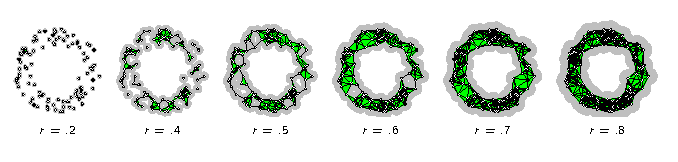
\includegraphics[width=\textwidth]{filtration}
\end{figure}
\noindent Compute how homology changes as we grow a space. 
\begin{figure}[h!]
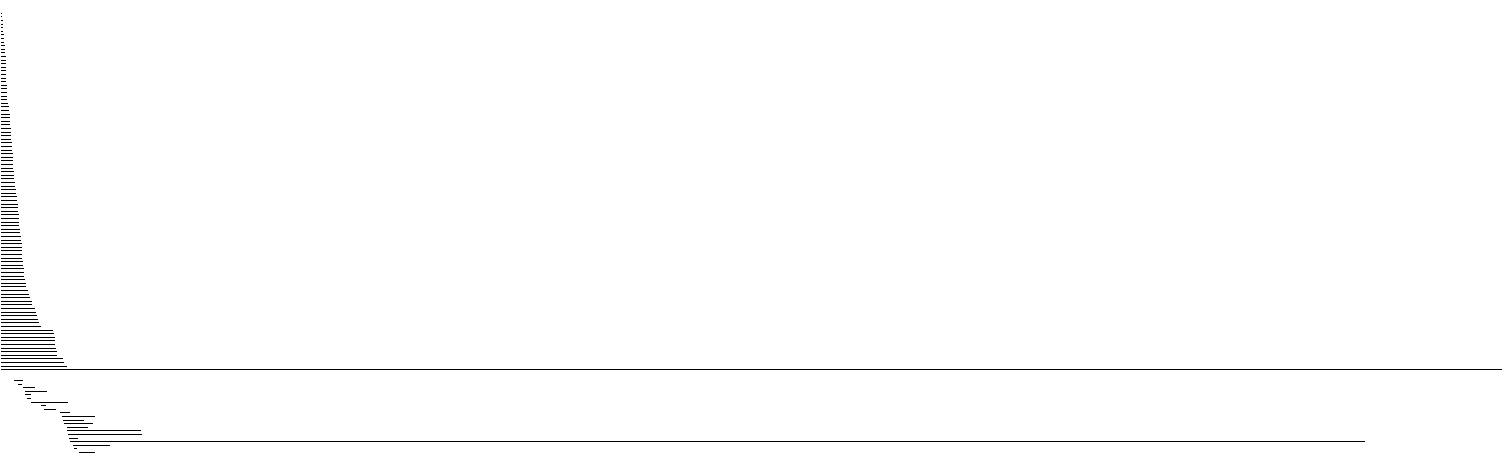
\includegraphics[width=\textwidth]{barcodes}
\end{figure}
Results are captured by a \emph{persistence diagram}
\vfill
\end{frame}

\begin{frame}[fragile]
\frametitle{Defining Homology}
\begin{figure}
\centering
\begin{tikzpicture}[scale=.33, every node/.style={scale=0.33}]
 \begin{axis} [axis lines=none,view={0}{60}]
            \addplot3 [surf,
                 draw=white,
                 fill=afragreen,
                shader=flat,
                domain = 0: 360, 
                 y domain = 0: 360, 
                 samples = 10, 
                  z buffer = sort, ultra thick]
            ( { (10+5*cos(x))*cos(y) } , 
             { (10+5*cos(x))*sin(y) } , 
             { 5*sin(x) } );
 \end{axis}
\node[scale=2] at (3,0) {$C_2$ vector space of faces}; 
\node[scale=5] at (9,4.5) {$\partial_2$};
 \begin{scope}[scale=.05, shift={(145,35)}]
  \path[draw=black,fill=afragreen, line width=2pt] (2.57,14.56) -- (1.9450, 33.7380) -- (63.8200,33.5230) -- (63.8200,47.7970) -- (107.5700,25.4260) -- (64.4450,3.0550) -- (63.8200,18.8240) -- (2.5700,14.5620);
  \end{scope}
  \node[scale=2] at (16,0) {$C_1$ vector space of edges}; 
\begin{scope}[shift={(13,0)}]
 \begin{axis} [axis lines=none,view={0}{60}]
            \addplot3 [surf,
                 draw=afragreen,
                 fill=white,
                shader=flat,
                domain = 0: 360, 
                 y domain = 0: 360, 
                 samples = 10, 
                  z buffer = sort, ultra thick]
            ( { (10+5*cos(x))*cos(y) } , 
             { (10+5*cos(x))*sin(y) } , 
             { 5*sin(x) } );
 \end{axis}
 \end{scope}
 \node[scale=2] at (29,0) {$C_0$ vector space of vertices}; 
\node[scale=5] at (22,4.5) {$\partial_1$};
 \begin{scope}[scale=.05, shift={(405,35)}]
  \path[draw=black,fill=afragreen, line width=2pt] (2.57,14.56) -- (1.9450, 33.7380) -- (63.8200,33.5230) -- (63.8200,47.7970) -- (107.5700,25.4260) -- (64.4450,3.0550) -- (63.8200,18.8240) -- (2.5700,14.5620);
  \end{scope}
 \begin{scope}[shift={(26,0)}]
 \begin{axis} [axis lines=none,view={0}{60}]
            \addplot3 [surf,
                 draw=white,
                 fill=white,
                shader=flat,
                domain = 0: 360, 
                 y domain = 0: 360, 
                 samples = 10, 
                 mark=*, mark options={solid, color=afragreen},  z buffer = sort, ultra thick]
            ( { (10+5*cos(x))*cos(y) } , 
             { (10+5*cos(x))*sin(y) } , 
             { 5*sin(x) } );
 \end{axis}
 \end{scope}
 \end{tikzpicture}
 \vfill
 Take the linear extension of the boundary operator:
\[ \partial_d([v_0, \ldots v_d]) = \sum_{i=0}^d (-1)^i [v_0 \ldots, \hat{v}_i, \ldots v_d] \]
\begin{description}
\item[Lemma: \phantom{6}]<3-> $\partial_{d-1} \circ \partial_{d} \equiv 0 \Rightarrow \im{ \partial_{d}} \subseteq \ker{\partial_{d-1}}$
\item[Definition:]<4-> $ H_d(K) = \ker{\partial_d} / \im{ \partial_{d+1}} $
\end{description}
\end{figure}
\end{frame}

\begin{frame}[fragile]
\frametitle{Homology}
\begin{figure}
\begin{tikzpicture}[scale=.75]
 \begin{axis} [axis lines=none,view={0}{60}]
            \addplot3 [surf,
                 draw=gray,
                 fill=afragreen,
                shader=flat,
                domain = 0: 360, 
                 y domain = 0: 360, 
                 samples = 40, 
                  z buffer = sort]
            ( { (\torusc+\torusa*cos(x))*cos(y) } , 
             { (\torusc+\torusa*cos(x))*sin(y) } , 
             { \torusa*sin(x) } );

%%horizontal generator
 \addplot3 [
     draw=blue,
     samples=40,
     domain=0:-180,
     ultra thick
    ] (
              {(\torusc + \torusa*cos(0))*cos(y)},
              {(\torusc + \torusa*cos(0))*sin(y)},
              {\torusa*sin(0)});
 %horizontal generator dashed         
\addplot3 [
     draw=blue,
     opacity=.5,
     samples=40,
     domain=-180:-360,
     ultra thick, dashed
    ] (
              {(\torusc + \torusa*cos(0))*cos(y)},
              {(\torusc + \torusa*cos(0))*sin(y)},
              {\torusa*sin(0)});
                          
        %vertical generator         
    \addplot3 [
      draw=red,
      samples=40,
      samples y=1,
      domain= 0:170,
      ultra thick
    ] (
              {\torusc + \torusa*cos(x)},
              {0},
              {\torusa*sin(x)});
      %vertical generator dashed           
    \addplot3 [
      draw=red,
      samples=40,
           opacity=.5,
      samples y=1,
      domain= 170:360,
      ultra thick, dashed
    ] (
              {\torusc + \torusa*cos(x)},
              {0},
              {\torusa*sin(x)});
 \end{axis}
\end{tikzpicture}
\caption{Homology of the torus $T^1$}
\end{figure}
Homology is a module (vector space over a ring)
\begin{center}
\begin{description}
\item<1->[$\betti_0 = \dim{H_0(T^1)}$] = 1 connected component
\item<2->[$\betti_1 = \dim{H_1(T^1)}$] = 2 loops around the donut hole.
\item<3->[$\betti_2 = \dim{H_2(T^1)}$] = 1 void (useful for jelly filling).
\end{description}
\end{center}
\end{frame}

\begin{frame}
\frametitle{Persistent Homology is the Homology of Maps}
\vspace{-1cm}
\begin{figure}
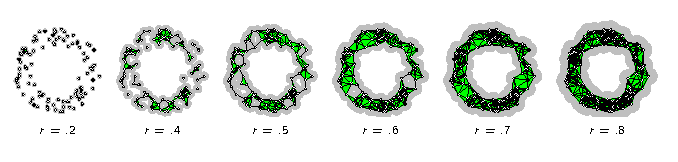
\includegraphics{filtration.pdf} \\
\only<4->{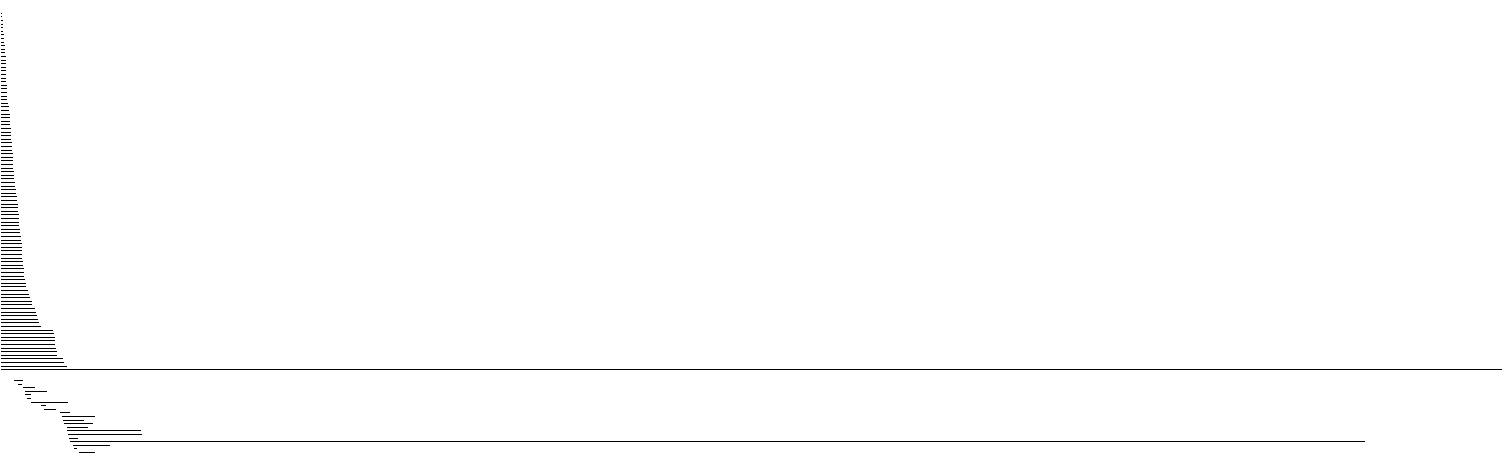
\includegraphics[height=80pt, width=400pt]{barcodes.pdf}}
    \end{figure}
\only<1-3>{\[ H_d(\check{C}_*) = \bigoplus_{\epsilon} H_d(\check{C}_{\epsilon}) \]}
\only<2-3>{
Carlsson and Zomorodian show us that when using field coefficients there is a structure theorem!
}
\only<3->{
\[ H_d(\check{C}_*) = \left( \bigoplus_{\alpha} t^{\alpha}k[t]\right) \bigoplus \left( \bigoplus_{[\alpha, \beta)} t^{\alpha}k[t]/t^\beta \right) \]
}
\only<4>{
\textbf{Next:} Explain factorization and a parallel persistence algorithm.
}
\end{frame}

%\begin{frame}{Exact Sequences \& Linear Algebra}
Suppose $A \subset X$ then we have:

\[ \begin{tikzcd}[ampersand replacement=\&, column sep=small]
0 \arrow{r} \& C_n(A) \arrow{r}{i} \& C_n(X) \arrow{r}{j} \& C_n(X/A) \arrow{r} \& 0
\end{tikzcd}
\]
This is \emph{exact} meaning that $\ker{j} = \im{i}$. \\
\vspace{.5cm}
When we compute homology we get a larger exact sequence:
\[ \begin{tikzcd}[ampersand replacement=\&, column sep=small]
\ldots \arrow{r}{\delta} \& H_n(A) \arrow{r}{i} \& H_n(X) \arrow{r}{j} \& H_n(X/A) \arrow{r}{\delta} \& H_{n-1}(A) \arrow{r}{i} \& \ldots 
\end{tikzcd}
\]
where:
\[ \delta_n([x]) = [\partial_n(x)] \]

\begin{center}
\textbf{This is the recipe for a basic parallel algorithm.}
\end{center}
\end{frame}
\begin{frame}{Exact Sequences \& Linear Algebra}
We can decompose $\partial_X$ the boundary matrix for $X$ as follows: 
\only<1>{
\[ \begin{blockmatrixtabular}
  \begin{blockmatrixtabular}
  \fblockmatrix     [0.8,1.0,0.8]{1.5in}{1.5in}{$\partial_A$}\\
  \fblockmatrix     [0.8,0.8,1.0]{1.5in}{1.5in}{$0$}
  \end{blockmatrixtabular}
  \begin{blockmatrixtabular}
  \fblockmatrix     [0.8,0.8,1.0]{1.5in}{1.5in}{$\tilde{\delta}$}\\
  \fblockmatrix     [1.0,0.8,0.8]{1.5in}{1.5in}{$\partial_{X/A}$}
  \end{blockmatrixtabular}
\end{blockmatrixtabular} 
\]
}
\only<2>{
\[ \begin{blockmatrixtabular}
  \begin{blockmatrixtabular}
  \fblockmatrix     [0.8,1.0,0.8]{1.5in}{1.5in}{$S_A \cdot P_A$}\\
  \fblockmatrix     [0.8,0.8,1.0]{1.5in}{1.5in}{$0$}
  \end{blockmatrixtabular}
  \begin{blockmatrixtabular}
  \fblockmatrix     [0.8,0.8,1.0]{1.5in}{1.5in}{$\delta = S_{X/A}\tilde{\delta}D_{X/A}$}\\
  \fblockmatrix     [1.0,0.8,0.8]{1.5in}{1.5in}{$P_{X/A}$}
  \end{blockmatrixtabular}
\end{blockmatrixtabular} 
\]
}
The algorithm becomes: 
\begin{enumerate}
\item<1-> Compute homology within each diagonal block (in parallel).
\begin{description}
\item \hspace*{-2cm} Factor $\partial_A = S_A \cdot P_A \cdot D_A$.  where $S$ and $D$ are invertible.
\item \hspace*{-2cm} Factor $\partial_{X/A} = S_{X/A} \cdot P_{X/A} \cdot D_{X/A}$.  
\end{description}
\item<2> Afterwords: reduce the map $\delta$.
\begin{description}
\item \hspace*{-2cm} For each nonzero column in $\delta$ whose reduce them against $S_AP_A$
\end{description}
\end{enumerate}
\end{frame}
\begin{frame}{Algorithm Analysis}
Assume $\card{A} = n$ and $\card{X} = m$

\begin{description}
\item<1->[Correctness] follows from exact sequence.
\item<2->[Complexity] $O((m-n)^3 + n^3 + (m-n) \cdot m \cdot n)$. 
\item<3->[Speedup] This is minimized when $n = \frac{m}{2}$ and at that point we have a speedup of 2.
\end{description}
\only<4>{How to correctly extend this to a sequence of subspaces \[ K_0 \subseteq K_1 \subseteq K_2 \subset \ldots \subset K_n \hspace{.25cm} ?\] }
\end{frame}


\begin{frame}{Homology from a filtration}
How to correctly extend this to a sequence of subspaces \[ K_0 \subseteq K_1 \subseteq K_2 \subset \ldots \subset K_n \hspace{.25cm} ?\] 
We can decompose $\partial_X$ the boundary matrix $X$ in a similar way: 
\[ \begin{blockmatrixtabular}
  \begin{blockmatrixtabular}
    \alt<1>{\greenbox{$\partial_0$}}{\bluebox{$\partial_0$}} \\
    \alt<1>{\bluebox{0}}{\bluebox{0}} \\
    \alt<1>{\bluebox{0}}{\bluebox{0}} \\
    \alt<1>{\bluebox{0}}{\bluebox{0}} \\
    \alt<1>{\bluebox{0}}{\bluebox{0}}
  \end{blockmatrixtabular}
  \begin{blockmatrixtabular}
    \alt<2>{\greenbox{$\tilde{d_0}$}}{\bluebox{$\tilde{d_0}$}} \\
    \alt<1>{\greenbox{$\partial_1$}}{\bluebox{$\partial_1$}} \\
    \alt<1>{\bluebox{0}}{\bluebox{0}} \\
    \alt<1>{\bluebox{0}}{\bluebox{0}} \\
    \alt<1>{\bluebox{0}}{\bluebox{0}}
  \end{blockmatrixtabular}
  \begin{blockmatrixtabular}   
    \alt<3>{\greenbox{$\tilde{d_0}$}}{\bluebox{$\tilde{d_0}$}} \\
    \alt<2>{\greenbox{$\tilde{d_0}$}}{\bluebox{$\tilde{d_0}$}} \\
    \alt<1>{\greenbox{$\partial_2$}}{\bluebox{$\partial_2$}} \\
    \alt<1>{\bluebox{0}}{\bluebox{0}} \\
    \alt<1>{\bluebox{0}}{\bluebox{0}}
  \end{blockmatrixtabular}
    \begin{blockmatrixtabular}
    \alt<4>{\greenbox{$\ldots$}}{\bluebox{$\ldots$}} \\
    \alt<3>{\greenbox{$\ldots$}}{\bluebox{$\ldots$}} \\
    \alt<2>{\greenbox{$\ldots$}}{\bluebox{$\ldots$}} \\
    \alt<1>{\greenbox{$\ldots$}}{\bluebox{$\ldots$}} \\
    \alt<1>{\bluebox{0}}{\bluebox{0}}
    \end{blockmatrixtabular}
    \begin{blockmatrixtabular}
    \alt<5>{\greenbox{$\tilde{d}_{n,n}$}}{\bluebox{$\tilde{d}_{n,n}$}} \\
    \alt<4>{\greenbox{$\tilde{d}_{n-1,n}$}}{\bluebox{$\tilde{d}_{n-1,n}$}} \\
    \alt<3>{\greenbox{$\tilde{d}_{\ldots,n}$}}{\bluebox{$\tilde{d}_{\ldots,n}$}} \\
    \alt<2>{\greenbox{$\tilde{d}_{0,n}$}}{\bluebox{$\tilde{d}_{0,n}$}} \\
    \alt<1>{\greenbox{$\partial_n$}}{\bluebox{$\partial_n$}} \\
  \end{blockmatrixtabular}
\end{blockmatrixtabular} 
\]
\only<6>{\textbf{Question: } How do you show correctness?}
\end{frame}


\begin{frame}{Spectral Sequence of A Filtration}
\only<1-5>{
\begin{figure}
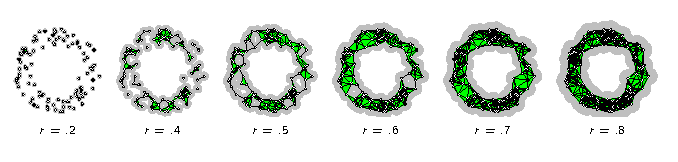
\includegraphics[width=\textwidth]{filtration}
\end{figure}
}
\only<1>{
From our sequence of spaces, we have a filtration of chain complexes:
\[ 
\begin{tikzcd}[ampersand replacement=\&, column sep=small]
0 \arrow{r}{i} \& C_*(K_0) \arrow{r}{i} \& C_*(K_1) \arrow{r}{i}    \& \ldots \arrow{r}{i} \& C_*(K_{n-1}) \arrow{r}{i} \& C_*(K_n) 
\end{tikzcd}
\]
}
\only<2>{
Attach the co-kernel to get short exact sequences
\[
\hspace*{-1cm}
\begin{tikzcd} [ampersand replacement=\&, column sep=small]
0 \arrow{r}{i} \&  C_*(K_0) \arrow{r}{i}\arrow{d}{j} \&  C_*(K_1) \arrow{r}{i}\arrow{d}{j}    \& \ldots \arrow{r}{i} \&  C_*(K_{n-1}) \arrow{r}{i} \arrow{d}{j} \&  C_*(K_n) \arrow{d}{j} \\ 	
\&     C_*(K_0,{0}) \&	C_*(K_1,{K_0}) \& \ldots  	 \& C_*(K_{n-1},{K_{n-2}})		 \& C_*(K_n,{K_{n-1}}) 
\end{tikzcd}
\]
}
\only<3-4>{
Pass to homology, where triangles are exact. \\
\[
\hspace*{-1cm}
\begin{tikzcd}[ampersand replacement=\&, column sep=small]
0 \arrow{r}{i} \& H(K_0 \arrow{r}{i}\arrow{d}{j}) \& H(K_1 \arrow{r}{i}\arrow{d}{j})    \& \ldots \arrow{r}{i} \& H(K_{n-1}) \arrow{r}{i} \arrow{d}{j} \& H(K_n\arrow{d}{j}) \\ 		
\&     H(K_0) \&	  \only<4>{\arrow{l}{d_{1}}} \arrow{ul}{\delta}  H(K_1, {K_0}) \& \only<4>{\arrow{l}{d_{1}}} \arrow{ul}{\delta} \hspace{.5cm} \ldots  	 \&\only<4>{\arrow{l}{d_{1}}}\arrow{ul}{\delta}H(K_{n-1}, {K_{n-2}})		 \& \only<4>{\arrow{l}{d_{1}}} \arrow{ul}{\delta} H(K_n, {K_{n-1}})
\end{tikzcd}
\]
\[  E^2 = H_*(d_1) \]
}
\only<5-6>{
Build a new chain complex by constructing $d_1 = j \circ \delta$ 
\[
\begin{tikzcd}[ampersand replacement=\&, column sep=small]
0 \arrow{r}{i} \& H(K_0 \arrow{r}{i}\arrow{d}{j}) \& H(K_1 \arrow{r}{i}\arrow{d}{j})    \& \ldots \arrow{r}{i} \& H(K_{n-1}) \arrow{r}{i} \arrow{d}{j} \& H(K_n\arrow{d}{j}) \\ 		
\&     E^2_0 \&	  \arrow{l}{0} \arrow{ul}{\delta}  E^2_1 \& \arrow{l}{0} \arrow[bend left]{ll}{d_{2}} \arrow{ul}{\delta} \hspace{.5cm} \ldots  	 \& \arrow{l}{0} \arrow[bend left]{ll}{d_{2}} \arrow{ul}{\delta}E^1_{n-1}	 \& \arrow{l}{0} \arrow[bend left]{ll}{d_{2}} \arrow{ul}{\delta} E_n
\end{tikzcd}
\]
\pause
More generally:
\[ d_{r,p}: E_{r+p} \rightarrow E_p \]
Eventually $d_{n,p} = 0$, when sequence has converged.  
}
\only<7->{
\[
\begin{tikzcd}[ampersand replacement=\&, column sep=small]
0 \arrow{r}{i} \& H(K_0 \arrow{r}{i}\arrow{d}{j}) \& H(K_1 \arrow{r}{i}\arrow{d}{j})    \& \ldots \arrow{r}{i} \& H(K_{n-1}) \arrow{r}{i} \arrow{d}{j} \& H(K_n\arrow{d}{j}) \\ 		
\&     E^\infty_0 \&	  \arrow{l}{0} \arrow{ul}{\delta}  E^\infty_1 \& \arrow{l}{0} \arrow{ul}{\delta} \hspace{.5cm} \ldots  	 \& \arrow{l}{0} \arrow{ul}{\delta}E^\infty_{n-1}	 \& \arrow{l}{0} \arrow{ul}{\delta} E^\infty_n
\end{tikzcd}
\]
The data on the final page is called the $E^\infty$ page.  \\
\pause
\begin{theorem}{Free Lunch}
\[ PH_*(K) \cong  \bigoplus_{r,p} t^p \operatorname{Im}(d_{r,p})/t^{p+r} \bigoplus_p t^p E^\infty_p \]
\end{theorem}
}
\end{frame}
\begin{frame}{Remarks}
\begin{itemize}
\item<1-> Clear connection to persistent homology
\item<2-> Easy to implement
\item<3-> \emph{Doesn't load balance well} (lose a useful thread at each step)
\item<4-> Data on each processor eventually coupled to every other processor.
\end{itemize}
\only<5>{Seek an algorithm which works on large parts of the space in parallel, with small intersections}
\end{frame}
%\begin{frame}[fragile]{Mayer Vietoris}
%\begin{figure}
%\begin{tikzpicture}[scale=.5, y=0.6pt, x=.75pt]
%     %row 1
%%     \node[font=\large] at (-50, 800) {$(K, U)$};
%     \draw[fill=afragreen, draw = black,  line width=2]  (47,800) circle (10pt);  
%     \draw[fill=afragreen, draw = black, line width=2]  (117,800) circle (10pt);   
%     \draw[fill=afragreen, draw = black, line width=2]  (190,800) circle (10pt); 
%     \draw[fill=afragreen, draw = black, line width=2]  (261,800) circle (10pt); 
%     \begin{pgfonlayer}{edges}
%            \path[draw=black,fill=black,line width=2] (47,800) -- (117, 800);
%            \path[draw=black,fill=black,line width=2] (117,800) -- (190, 800);
%            \path[draw=black,fill=black,line width=2] (190,800) -- (261, 800);
%      \end{pgfonlayer}      
%      \draw[draw, color=afrablue, fill=none, line join=round,draw opacity=0.978,line width=2] (117, 800) ellipse (100 and 45) node[anchor=north, xshift=-.55in] {$U_0$};
%      \draw[draw, color=afrapurple, fill=none, line join=round,draw opacity=0.978,line width=2] (190, 800) ellipse (100 and 45) node[anchor=north, xshift=.6in] {$U_1$};
%    \end{tikzpicture}
%\caption{Space and Cover}
%\label{fig:space-n-cover}
%\end{figure}
%
%When we have a pair of sets there is another short exact sequence:
%\begin{tikzcd}
% C_*(U_0 \cap U_1) \hspace{1mm} \arrow{r}{x \mapsto (x,x)} & C_*(U_0) \bigoplus C_*(U_1) \hspace{1mm} \arrow{r}{ (x,y) \mapsto x-y} & \hspace{1mm} C_*(U_0 \bigcup U_1) = C_*(X) \\
% \end{tikzcd}
%When you have intersections of 3 or more sets, this becomes the mayer vietoris spectral sequence, with the following initial data:
%\[ E^0_{p,q} = \langle p\text{-chains in a }q\textrm{-way intersection} \rangle \]
%\pause
%We will come back to this. For now, lets take advantage of this covering.
%\end{frame}

%\begin{frame}[fragile]
%\frametitle{Compute homology via subcomplexes}
%\begin{minipage}{.35\textwidth}
%\begin{tikzpicture}[scale=.5, y=0.6pt, x=.75pt]
%     %row 1
%%     \node[font=\large] at (-50, 800) {$(K, U)$};
%     \draw[fill=afragreen, draw = black,  line width=2]  (47,800) circle (10pt);  
%     \draw[fill=afragreen, draw = black, line width=2]  (117,800) circle (10pt);   
%     \draw[fill=afragreen, draw = black, line width=2]  (190,800) circle (10pt); 
%     \draw[fill=afragreen, draw = black, line width=2]  (261,800) circle (10pt); 
%     \begin{pgfonlayer}{edges}
%            \path[draw=black,fill=black,line width=2] (47,800) -- (117, 800);
%            \path[draw=black,fill=black,line width=2] (117,800) -- (190, 800);
%            \path[draw=black,fill=black,line width=2] (190,800) -- (261, 800);
%      \end{pgfonlayer}      
%      \draw[draw, color=afrablue, fill=none, line join=round,draw opacity=0.978,line width=2] (117, 800) ellipse (100 and 45) node[anchor=north, xshift=-.55in] {$U_0$};
%      \draw[draw, color=afrapurple, fill=none, line join=round,draw opacity=0.978,line width=2] (190, 800) ellipse (100 and 45) node[anchor=north, xshift=.6in] {$U_1$};
%    \end{tikzpicture}
%Space and Cover
%\end{minipage}
%\begin{minipage}{.2\textwidth}
%\begin{tikzpicture}[y=1.0pt, x=0.8pt, yscale=-1, scale=.5]
%      \path[draw=black,fill=afragreen, line width=3pt,transform canvas={xshift = 1cm}] (2.57,14.56) -- (1.9450, 33.7380) -- (63.8200,33.5230) -- (63.8200,47.7970) -- (107.5700,25.4260) -- (64.4450,3.0550) -- (63.8200,18.8240) -- (2.5700,14.5620);
%\end{tikzpicture}
%\vspace*{1cm}
%\end{minipage}
%\begin{minipage}{.4\textwidth}
%\begin{tikzpicture}[scale=.5, y=0.6pt, x=.75pt]
%    %disj 0
%    \begin{scope}[shift={(143,80)}]
%    \node[font=\large] at (300, 730) {$K^0 \times \Delta^{0}$};
%     \draw[draw, color=afrablue, fill=none, line join=round,draw opacity=0.978,line width=2] (117, 730) ellipse (100 and 45);
%     \draw[fill=afrablue, draw = black, line width=2]  (47,730) circle (10pt);  
%     \draw[fill=afrablue, draw = black, line width=2]  (117,730) circle (10pt);   
%     \draw[fill=afrablue, draw = black, line width=2]  (190,730) circle (10pt); 
%     \begin{pgfonlayer}{edges}
%            \path[draw=black,fill=black,line width=2] (47,730) -- (117, 730);
%            \path[draw=black,fill=black,line width=2] (117,730) -- (190, 730);
%      \end{pgfonlayer}   
%      \end{scope}
%      %disj  1
%       \begin{scope}[shift={(0,0)}]
%        \node[font=\large] at (380, 680) {$K^1 \times \Delta^{1}$};
%       \draw[draw, color=afrapurple, fill=none, line join=round,draw opacity=0.978,line width=2] (190, 680) ellipse (100 and 45);
%     \draw[fill=afrapurple, draw = black, line width=2]  (117,680) circle (10pt);   
%     \draw[fill=afrapurple, draw = black, line width=2]  (190,680) circle (10pt); 
%      \draw[fill=afrapurple, draw = black, line width=2]  (261,680) circle (10pt); 
%         \begin{pgfonlayer}{edges}
%            \path[draw=black,fill=black,line width=2] (117,680) -- (190, 680);
%            \path[draw=black,fill=black,line width=2] (190,680) -- (261, 680);
%      \end{pgfonlayer}   
%            \end{scope}
%      %blowup edges 
%      \begin{scope}[shift={(143,80)}]
%     \begin{pgfonlayer}{edges}
%            \path[draw=black,fill=black,line width=2] (47,730) -- (47, 600);
%            \path[draw=black,fill=black,line width=2] (117,730) -- (117, 600);
%      \end{pgfonlayer}     
%          \node[font=\large] at (280, 665) {$K^{[1]} \times \Delta^{[1]}$};
%        \begin{pgfonlayer}{quadcell}
%      \draw [fill=afragreen,  preaction={fill, afragreen}, pattern=north west lines, pattern color=black] (47, 600) rectangle (117, 730);
%	\end{pgfonlayer}
%	\end{scope}
%\end{tikzpicture}
%The blowup complex.
%\end{minipage}
%{\color{blue}{Definition:}} \[ K^{U} = \bigcup_{J \in N(U)} U_J \times J \]
%where $U_J = \bigcap_{j \in J} U_j$ and $N(U)$ is the nerve of $U$.
%\pause
%\begin{theorem}[Segal]
%For any closed cover $U$, $K^U$ and $K$ are homotopy equivalent.
%\end{theorem}
%\pause \textbf{Recipe for a parallel \emph{homology} algorithm}
%\end{frame}
%\begin{frame}
\frametitle{Parallel Algorithm}
\begin{figure}[t]
\def\svgwidth{.8\textwidth} 
\input{images/blowup-persistence.pdf_tex}
\end{figure}
\hspace{-.5cm}\textbf{Algorithm:}
\begin{itemize} 
	\item<1->[Step 1:] Compute the homology of each local piece (in parallel)
	\item<2->[Step 2:] Compute the homology with the blowup pieces (in serial)
\end{itemize}
\only<3->{
\hspace{-.5cm} \textbf{Goal:} 
\begin{itemize}
	\item Do most of work Step 1, Do as little as possible in Step 2.
	\item Equivalent to \textit{quickly} generating ``balanced'' and 
		``minimal'' covers.
\end{itemize}
}
\end{frame}

\begin{frame}
\frametitle{Finding Minimum Blowups}
\textbf{Goal:} Quickly generate cover, $\U$, with balanced size and ``minimal''
overlap.  \\
\vspace{.1cm}
\pause
\textbf{Formally:} 
Given $\alpha \in (\frac{1}{n},1)$ find a covering 
$\U = \{ \U_1, \ldots, \U_n \}$ minimizing: 
\[ \frac{\card{K^\U}}{\card{K}} \] \pause 
subject to:  
\[ \max_{i\in[n-1]}{\card{\U_{i}}} \leq \alpha \card{K} \] \pause 
\end{frame}

\begin{frame}
\frametitle{Finding Minimum Blowups} 
\textbf{Bad News:}
\begin{itemize}
\item<1-> $\frac{\card{K^\U}}{\card{K}}$ is \emph{at worst exponential} in
	$\card{U}$ 
\item<2-> We prove finding $\alpha$-balanced Minimal Blowups is
	$\mathsf{NP}$-Hard.
\end{itemize}
\only<3->{\textbf{Good News:}}
\begin{itemize}
\item<3-> Any cover gives us correct results. 
\item<4-> Approximate minimal blowups should still parallelize well.
\item<5-> We provide a heuristic algorithm with:
	\only<6-> {
		\[ \factor < 3 \]
		guaranteed!
	}
\end{itemize}
\end{frame}

	
%%%%%%%%%%%%%%%%%%%%%%%%%%%%%%%%%%
\begin{frame}
\frametitle{Cover Generation Algorithm}
\begin{itemize}
\item \textbf{Input: } Simplicial Complex $K$, and number of cover sets $n$
\item \textbf{Output:} Covering $\U$ into $n$ cover sets.
\end{itemize}
\begin{figure}
\def\svgwidth{.55\textwidth} 
\only<1>{\includesvg{images/algorithm_1}
\caption{Input Complex}}

\only<2>{\includesvg{images/algorithm_2}
\caption{Extract Graph of complex}}

\only<3>{\includesvg{images/algorithm_3}
\caption{Find partition of graph's vertex set (minimize edgecut)}}

\only<4>{\includesvg{images/algorithm_4}
\caption{Find partition (open cover) of complex}}

\only<5>{\includesvg{images/algorithm_5}
\caption{Close the extra set}}

%\only<6->{\includesvg{images/algorithm_6}
%\caption{(Optional) Union last set}}

\end{figure}
\end{frame}

\begin{frame}{Input Datasets}
\begin{itemize}
	\item Connected Cliques ({\multiblob}) $46 \times 10^6$ Dim: $10$
	\item Clique ({\clique}) $1 \times 10^6$ Dim: $19$
	\item Stanford Bunny ({\bunny}) $9.7 \times 10^6$ Dim: $3$
	\item Sphere ({\sphere}) $19 \times 10^6$ Dim: $8$
	\item {\Erdos}-{\Renyi} Random ({\gnp}) $3.6 \times 10^6$ Dim: $4$
\end{itemize}
\begin{figure}
	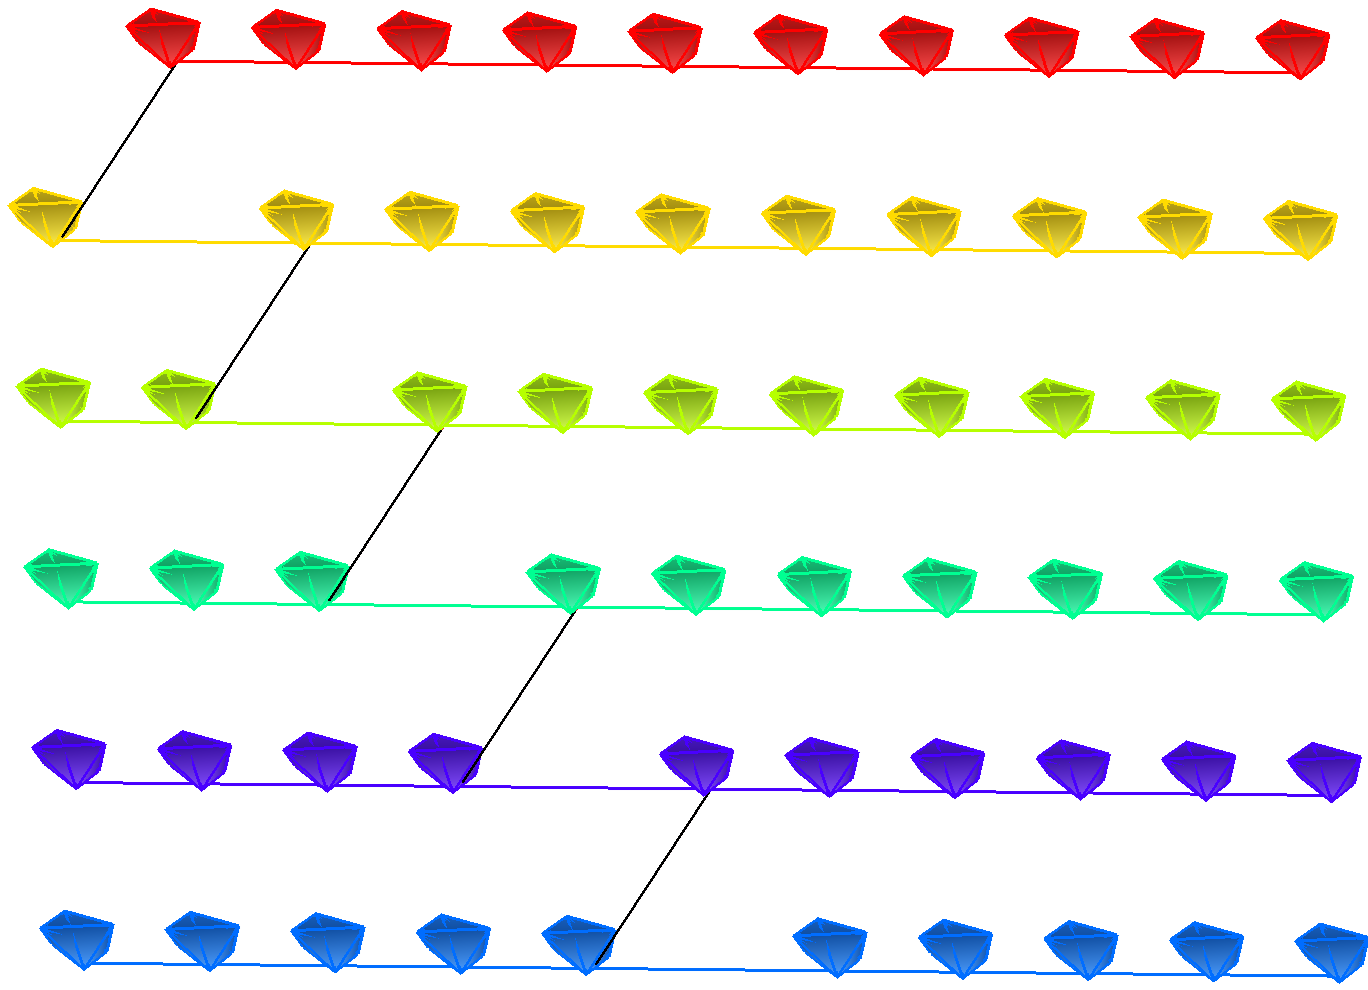
\includegraphics[width=.25\textwidth]{embedding.png}
	\hfill
	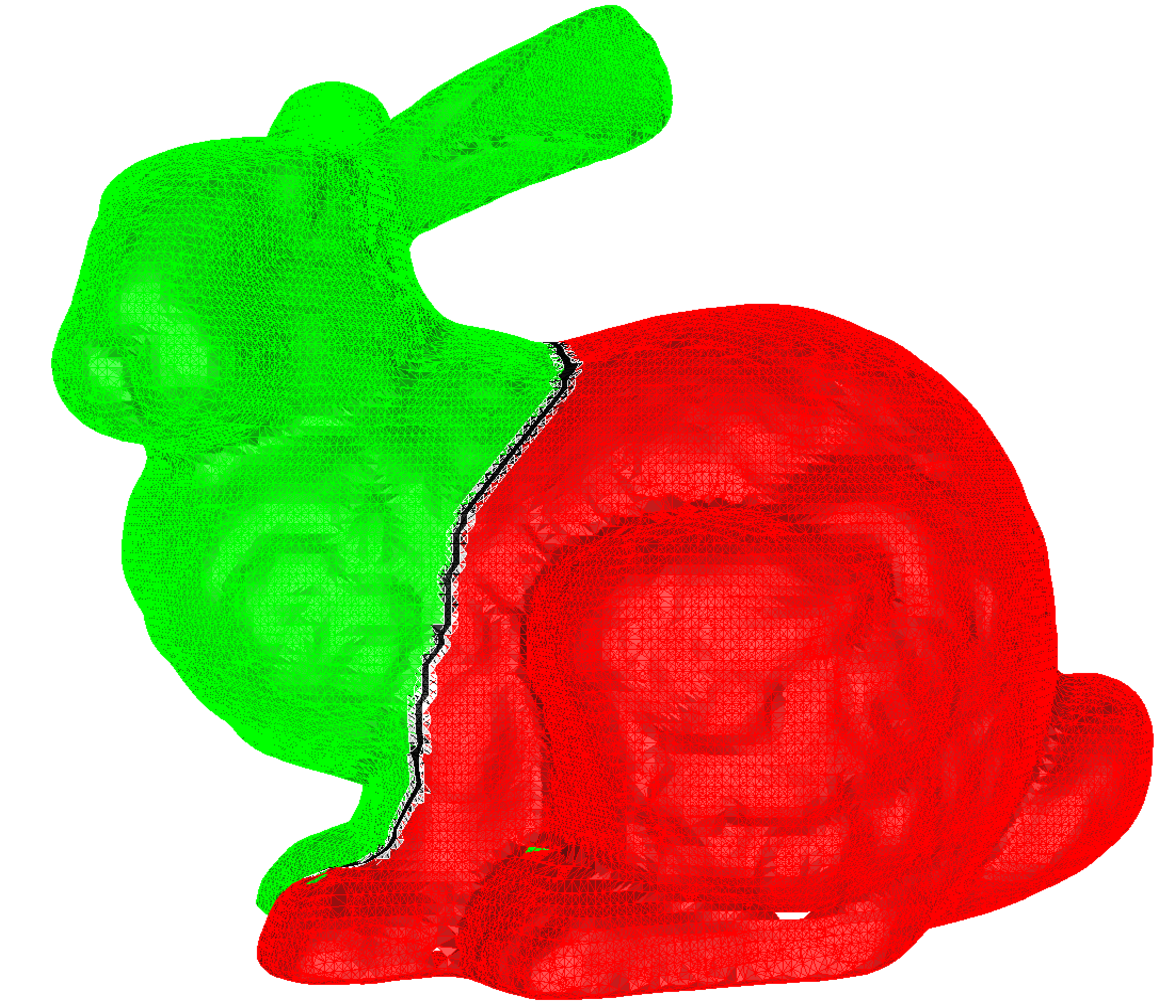
\includegraphics[width=.25\textwidth]{bunny-2.pdf}
	\hfill
	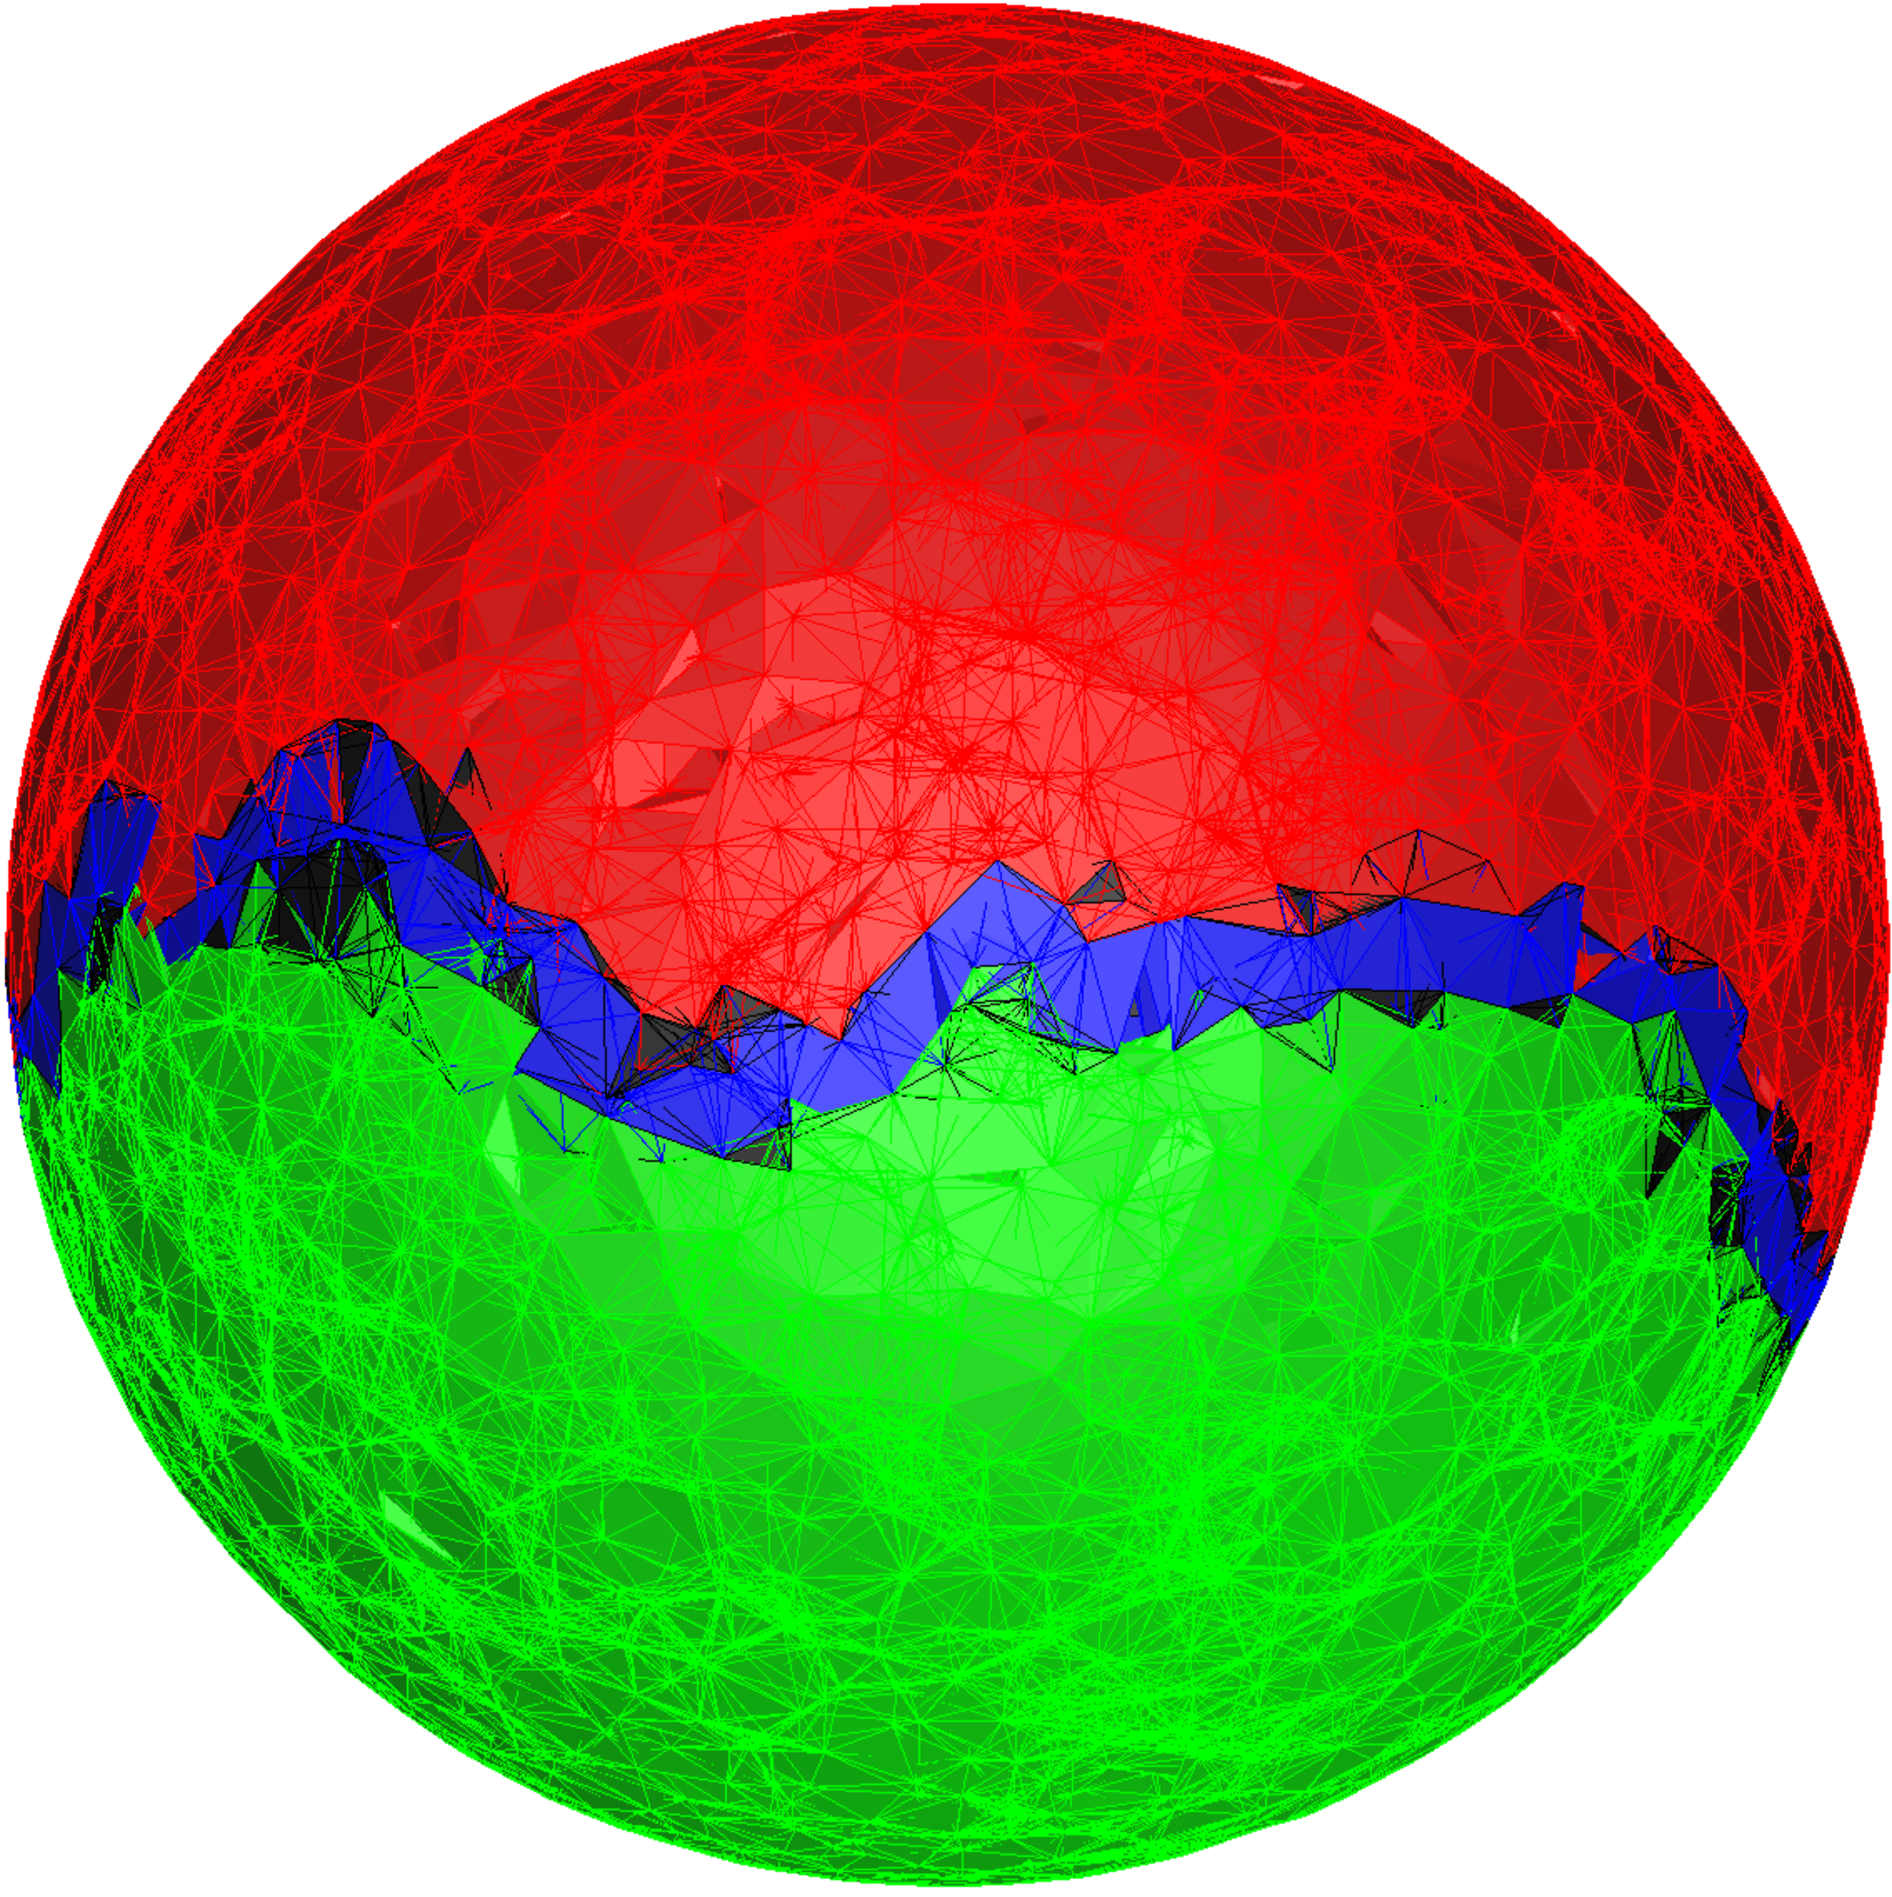
\includegraphics[width=.25\textwidth]{sphere-2.pdf}
\caption{Visualizations of {\multiblob}, {\bunny}, {\sphere}}
\end{figure}
\end{frame}

\begin{frame}
\begin{minipage}{.5\textwidth}
\centering
\begin{figure}
\centering
\begin{tikzpicture}[scale=.525]
\begin{axis}[xlabel=\# of partitions, ylabel={$\hat{\alpha}= \max_i \card{P_i} / \card{\K}$}, legend style={legend pos=north east, font=\small}]
\legend{\multiblob, \bunny, \clique, \gnp, \sphere, ideal}
\addplot table [x=num_partitions, y=graph_balance_ratio, col sep=comma] {pgf-speedup-figs/results/concurrent_homology/clique.11.22720.csv};
\addplot table [x=num_partitions, y=graph_balance_ratio, col sep=comma] {pgf-speedup-figs/results/concurrent_homology/bunny..05.csv};
\addplot table [x=num_partitions, y=graph_balance_ratio, col sep=comma] {pgf-speedup-figs/results/concurrent_homology/clique.20.csv};
\addplot table [x=num_partitions, y=graph_balance_ratio, col sep=comma] {pgf-speedup-figs/results/concurrent_homology/gnp.1250.047.csv};
\addplot table [x=num_partitions, y=graph_balance_ratio, col sep=comma] {pgf-speedup-figs/results/concurrent_homology/sphere.csv};
\addplot[dash pattern=on 4pt off 1pt on 4pt off 4pt, domain=2:10]{1/x};
\end{axis}
\end{tikzpicture}
\caption{Partition Balance Ratio $\hat{\alpha}$}
\end{figure}
\end{minipage}
\begin{minipage}{.5\textwidth}
\begin{figure}
\centering
\begin{tikzpicture}[scale=.525]
%\pgfplotsset{ymax=5}
\begin{axis}[xlabel=\# of partitions, ymax=50000, ylabel={\# of edges}, legend style={legend pos=north west, font=\small}]
\legend{\multiblob, \bunny, \clique, \gnp, \sphere, ideal}
\addplot table [x=num_partitions, skip coords between index={0}{1}, y=edgecut, col sep=comma, ignore chars=']
{pgf-speedup-figs/results/concurrent_homology/clique.11.22720.csv};
\addplot table [x=num_partitions, skip coords between index={0}{1}, y=edgecut, col sep=comma, ignore chars=']
{pgf-speedup-figs/results/concurrent_homology/bunny..05.csv};
\addplot table [x=num_partitions, skip coords between index={0}{1}, y=edgecut, col sep=comma, ignore chars=']
{pgf-speedup-figs/results/concurrent_homology/clique.20.csv};
\addplot table [x=num_partitions, skip coords between index={0}{1}, y=edgecut, col sep=comma, ignore chars=']
{pgf-speedup-figs/results/concurrent_homology/gnp.1250.047.csv};
\addplot table [x=num_partitions, skip coords between index={0}{1}, y=edgecut, col sep=comma, ignore chars=']
{pgf-speedup-figs/results/concurrent_homology/sphere.csv};
\end{axis}
\end{tikzpicture}
\caption{Edgecut}
\end{figure}
\end{minipage}
\begin{minipage}{.5\textwidth}
\centering
\begin{figure}
\begin{tikzpicture}[scale=.525]
\begin{axis}[xlabel=\# of partitions, ylabel={$\alpha = \max_i \card{\C_i} / \card{\K}$}, legend style={legend pos=north east, font=\small},legend style={at={(.95,.55)},anchor=east}]
\legend{\multiblob, \bunny, \clique, \gnp, \sphere, ideal}
\addplot table [x=num_partitions, y=cover_balance_ratio, col sep=comma,skip coords between index={0}{1}] 
{pgf-speedup-figs/results/concurrent_homology/clique.11.22720.csv};
\addplot table [x=num_partitions, y=cover_balance_ratio, col sep=comma, skip coords between index={0}{1}] 
{pgf-speedup-figs/results/concurrent_homology/bunny..05.csv};
\addplot table [x=num_partitions,skip coords between index={0}{1}, y=cover_balance_ratio, col sep=comma] 
{pgf-speedup-figs/results/concurrent_homology/clique.20.csv};
\addplot table [x=num_partitions, skip coords between index={0}{1},y=cover_balance_ratio, col sep=comma] 
{pgf-speedup-figs/results/concurrent_homology/gnp.1250.047.csv};
\addplot table [x=num_partitions, skip coords between index={0}{1},y=cover_balance_ratio, col sep=comma] 
{pgf-speedup-figs/results/concurrent_homology/sphere.csv};
\addplot[dash pattern=on 4pt off 1pt on 4pt off 4pt, domain=2:10]{1/x};
\end{axis}
\end{tikzpicture}
\caption{Balance Ratio for $\C$}
\end{figure}
\end{minipage}
\begin{minipage}{.5\textwidth}
\begin{figure}
\centering
\begin{tikzpicture}[scale=.525]
\begin{axis}[xlabel=\# of partitions, ylabel=$\ratio$, legend style={legend pos=north east, font=\small},legend style={at={(.95,.55)},anchor=east}]
\legend{\multiblob, \bunny, \clique, \gnp, \sphere, worst case}
\addplot table [x=num_partitions, y=blowup_factor, col sep=comma,skip coords between index={0}{1}] 
{pgf-speedup-figs/results/concurrent_homology/clique.11.22720.csv};
\addplot table [x=num_partitions, y=blowup_factor, col sep=comma, skip coords between index={0}{1}] 
{pgf-speedup-figs/results/concurrent_homology/bunny..05.csv};
\addplot table [x=num_partitions,skip coords between index={0}{1}, y=blowup_factor, col sep=comma] 
{pgf-speedup-figs/results/concurrent_homology/clique.20.csv};
\addplot table [x=num_partitions, skip coords between index={0}{1},y=blowup_factor, col sep=comma] 
{pgf-speedup-figs/results/concurrent_homology/gnp.1250.047.csv};
\addplot table [x=num_partitions, skip coords between index={0}{1},y=blowup_factor, col sep=comma] 
{pgf-speedup-figs/results/concurrent_homology/sphere.csv};
\addplot[dash pattern=on 4pt off 1pt on 4pt off 4pt, domain=2:10]{3};
\end{axis}
\end{tikzpicture}
\caption{Blowup Factor}
\label{fig:blowup-factors}
\end{figure}
\end{minipage}
\end{frame}

\begin{frame}
\begin{figure}
\centering
\begin{tikzpicture}[scale=.55]
\begin{semilogyaxis}[
name=plot1,
ymin=.09,
ymax=25,
xmin=0,
xmax=12,
xlabel=\# of  threads, 
title={$Multicore-Homology$},
ylabel= time to reduce boundary matrix (seconds),
minor y tick num={5},
legend style={at = {(.25,.6)}, font=\large}]
%\legend{\multiblob, \bunny, \clique, \gnp, \sphere}
\addplot table [x=num_threads, y=persistence, col sep=comma] {pgf-speedup-figs/results/concurrent_homology/clique.11.22720.csv};
\addplot table [x=num_threads, y=persistence, col sep=comma] {pgf-speedup-figs/results/concurrent_homology/bunny..05.csv};
\addplot table [x=num_threads, y=persistence, col sep=comma] {pgf-speedup-figs/results/concurrent_homology/clique.20.csv};
\addplot table [x=num_threads, y=persistence, col sep=comma] {pgf-speedup-figs/results/concurrent_homology/gnp.1250.047.csv};
\addplot table [x=num_threads, y=persistence, col sep=comma] {pgf-speedup-figs/results/concurrent_homology/sphere.csv};
\end{semilogyaxis}
\begin{semilogyaxis}[
name=plot3,
at=(plot1.below south east), anchor=above north east,
ymin=.09,
ymax=25,
xmin=0,
xmax=12,
xlabel= \# of threads,
title={$Heuristic-MH$},
%ylabel= time to reduce boundary matrix (seconds),
minor y tick num={5},
legend style={at={(1,.55)}, font=\large}]
%\legend{\multiblob, \bunny, \clique, \gnp, \sphere}
\addplot table [x=num_partitions, y=persistence, col sep=comma] {pgf-speedup-figs/results/cover_homology/clique.11.22720.csv};
\addplot table [x=num_partitions, y=persistence, col sep=comma] {pgf-speedup-figs/results/cover_homology/bunny..05.csv};
\addplot table [x=num_partitions, y=persistence, col sep=comma] {pgf-speedup-figs/results/cover_homology/clique.20.csv};
\addplot table [x=num_partitions, y=persistence, col sep=comma] {pgf-speedup-figs/results/cover_homology/gnp.1250.047.csv};
\addplot table [x=num_partitions, y=persistence, col sep=comma] {pgf-speedup-figs/results/cover_homology/sphere.csv};
\end{semilogyaxis}

\begin{semilogyaxis}[
name=plot4,
at=(plot3.right of north east), anchor=left of north west,
ymin=.09,
ymax=25,
xmin=0,
xmax=12,
xlabel= \# of threads, 
title={$Spectral-Sequence$},
minor y tick num={5},
legend style={at={(.95,.525)}, font=\large}]
\legend{\multiblob, \bunny, \clique, \gnp, \sphere}
\addplot table [x=num_partitions, y=persistence, col sep=comma] {pgf-speedup-figs/results/phat_14_ss/clique.11.22720.csv};
\addplot table [x=num_partitions, y=persistence, col sep=comma] {pgf-speedup-figs/results/phat_14_ss/bunny..05.csv};
\addplot table [x=num_partitions, y=persistence, col sep=comma] {pgf-speedup-figs/results/phat_14_ss/clique.20.csv};
\addplot table [x=num_partitions, y=persistence, col sep=comma] {pgf-speedup-figs/results/phat_14_ss/gnp.1250.047.csv};
\addplot table [x=num_partitions,, y=persistence, col sep=comma] {pgf-speedup-figs/results/phat_14_ss/sphere.csv};
\end{semilogyaxis}

\begin{semilogyaxis}[
name=plot2,
at=(plot4.above north west),
anchor = below south west,
ymin=.09,
ymax=25,
xmin=0,
xmax=12,
xlabel=\# of  threads,
title={$Chunk$},
minor y tick num={5},
legend style={at={(.95,.525)}, font=\large}]
%\legend{\multiblob, \bunny, \clique, \gnp, \sphere}
\addplot table [x=num_partitions, y=persistence, col sep=comma] {pgf-speedup-figs/results/phat_14_chunk/clique.11.22720.csv};
\addplot table [x=num_partitions, y=persistence, col sep=comma] {pgf-speedup-figs/results/phat_14_chunk/bunny..05.csv};
\addplot table [x=num_partitions, y=persistence, col sep=comma] {pgf-speedup-figs/results/phat_14_chunk/clique.20.csv};
\addplot table [x=num_partitions, y=persistence, col sep=comma] {pgf-speedup-figs/results/phat_14_chunk/gnp.1250.047.csv};
\addplot table [x=num_partitions,, y=persistence, col sep=comma] {pgf-speedup-figs/results/phat_14_chunk/sphere.csv};
\end{semilogyaxis}
\end{tikzpicture}
\caption{Time to reduce the boundary matrix for each algorithm.}
\label{fig:ctl_vs_phat}
\end{figure}

\end{frame}
%
%\begin{frame}
%\frametitle{Compute \emph{persistent} homology via subcomplexes}
%So far computes homology, but, not persistent homology. 
%\begin{figure}
%\begin{minipage}[t]{.35\textwidth}
%\coverfilt
% \end{minipage}
%\begin{minipage}{.2\textwidth}
%\begin{tikzpicture}[y=1.0pt, x=0.8pt, yscale=-1, scale=.5]
%      \path[draw=black,fill=afragreen, line width=3pt] (2.57,14.56) -- (1.9450, 33.7380) -- (63.8200,33.5230) -- (63.8200,47.7970) -- (107.5700,25.4260) -- (64.4450,3.0550) -- (63.8200,18.8240) -- (2.5700,14.5620);
%\end{tikzpicture}
%\vspace*{1cm}
%\end{minipage}
%\begin{minipage}[t]{.35\textwidth}
%\cover
%\end{minipage}
%\end{figure}
%%second row
%\pause
%\vspace{-1cm}
%\begin{figure}
%\begin{minipage}[t]{.35\textwidth}
%\disjointunion
% \end{minipage}
%\begin{minipage}{.2\textwidth}
%\begin{tikzpicture}[y=1.0pt, x=0.8pt, yscale=-1, scale=.5]
%      \path[draw=black,fill=afragreen, line width=3pt] (2.57,14.56) -- (1.9450, 33.7380) -- (63.8200,33.5230) -- (63.8200,47.7970) -- (107.5700,25.4260) -- (64.4450,3.0550) -- (63.8200,18.8240) -- (2.5700,14.5620);
%\end{tikzpicture}
%\vspace*{1cm}
%\end{minipage}
%\begin{minipage}[t]{.35\textwidth}
%\blowupcomplex
%\end{minipage}
%\end{figure}
%\vspace{-1cm}
%%second row
%\pause
%\begin{figure}
%\begin{minipage}[t]{.35\textwidth}
%\partialblowup
%\end{minipage}
%\begin{minipage}{.2\textwidth}
%\begin{tikzpicture}[y=1.0pt, x=0.8pt, yscale=-1, scale=.5]
%      \path[draw=black,fill=afragreen, line width=3pt] (2.57,14.56) -- (1.9450, 33.7380) -- (63.8200,33.5230) -- (63.8200,47.7970) -- (107.5700,25.4260) -- (64.4450,3.0550) -- (63.8200,18.8240) -- (2.5700,14.5620);
%\end{tikzpicture}
%\vspace*{1cm}
%\end{minipage}
%\begin{minipage}[t]{.4\textwidth}
%\blowupcomplex
%\end{minipage}
%\end{figure}
%\vspace{-1cm}
%\begin{itemize}
%\item[Issue:]<3-> Top filtration unrelated to a possible input filtration.
%\item[Issue:]<4-> Direct use of bottom filtration is not parallel.
%\item[Idea:]<5-> Re-examine the underlying spectral sequence
%\end{itemize}
%\end{frame}
%\begin{frame}[fragile]
%\frametitle{Mayer Vietoris Spectral Sequence}
%\begin{figure}[h]
%\centering
%\begin{tikzcd}[scale=1,
%execute at end scope={
%\only<2>{
%\begin{pgfonlayer}{edges}
%\node[xshift=-1em,yshift=.5em] (c2) at (e20.north west) {\footnotesize$C_2\left(K^{U}\right)$};
%\node[xshift=-1em,yshift=.5em] (c1) at (e10.north west) {\footnotesize$C_1\left(K^{U}\right)$};
%\node[xshift=-1em,yshift=.5em] (c0) at (e00.north west) {\footnotesize$C_0\left(K^{U}\right)$};
%\draw[opacity=.5,line width=7mm,line cap=round,color=afrablue] (e20.center) to (e02.center); 
%\draw[opacity=.5,line width=7mm,line cap=round,color=afragreen] (e10.center) to (e01.center); 
%\draw[opacity=.5,line width=7mm,line cap=round,color=afrapurple] (e00.center) to (e00.center);
%\end{pgfonlayer} 
%}}]
%|[alias=e30]|  \vdots \arrow{d}{\partial_{K}}& |[alias=e31]| \vdots \arrow{d}{\partial_{K}}& |[alias=e32]| \vdots \arrow{d}{\partial_{K}} \\
%|[alias=e20]|E^0_{2,0}  \arrow{d}{\partial_{K}}                     &  |[alias=e21]| E^0_{2,1} \arrow{l}{\partial_{N}} \arrow{d}{\partial_{K}}&|[alias=e22]|  E^0_{2,2} \arrow{l}{\partial_{N}}  \arrow{d}{\partial_{K}}& \ldots \arrow{l}{\partial_{N}} \\ 
%|[alias=e10]|E^0_{1,0} \arrow{d}{\partial_{K}}                     & |[alias=e11]| E^0_{1,1} \arrow{l}{\partial_{N}}  \arrow{d}{\partial_{K}}& |[alias=e12]| E^0_{1,2} \arrow{l}{\partial_{N}} \arrow{d}{\partial_{K}}& \ldots \arrow{l}{\partial_{N}} \\
%|[alias=e00]|E^0_{0,0}                                      & |[alias=e01]| E^0_{0,1} \arrow{l}{\partial_{N}}                & |[alias=e02]| E^0_{0,2} \arrow{l}{\partial_{N}}                   & \ldots \arrow{l}{\partial_{N}} 
%\end{tikzcd}
%\end{figure}
%\[ E^0_{p,q} = \langle p\text{-chains in a }q\textrm{-way intersection} \rangle \]
%\pause
%We can construct the blowup \emph{chain complex} where $ C_d = \bigoplus_{p+q=d} E^0_{p,q}$
%\pause
%The first two differentials:
%\[ d_0 = \partial_K \textrm{ and } d_1 = \partial_N \]
%\pause 
%Let's try an example!
%\end{frame}
\begin{frame}{Example: $S^1 \star S^1$}
\[
\begin{tikzpicture}[y=0.20pt, x=0.20pt, yscale=-1.000000, xscale=1.000000, inner sep=0pt, outer sep=0pt]
  \draw[xscale=1.000,yscale=-1.000,draw=black,even odd rule, line width=2pt] (335,-517.0366) circle (175); 
      \draw[xscale=1.000,yscale=-1.000,draw=black,even odd rule, line width=2pt] (565,-517.0366) node {$\star$};
 
    \path [draw=afragreen,  fill=none, fill opacity = 0.65,xscale=1.000,yscale=-1.000,even odd rule, line width=2pt] (825,-517.0366) circle (195);
             \draw[xscale=1.000,yscale=-1.000,draw=black,even odd rule, line width=2pt] (825,-517.0366) circle (175);
    \path [draw=afrablue,fill=none, fill opacity = 0.8,xscale=1.000,yscale=-1.000,even odd rule, line width=2pt] (825,-517.0366) circle (210);
       \path [draw=afrapurple, fill=none, fill opacity = 0.8,xscale=1.000,yscale=-1.000,even odd rule, line width=2pt] (825,-517.0366) circle (230);
      
  \path[fill=afrablue,opacity=0.6,line join=miter,line cap=butt,even odd
    rule,line width=0.800pt] (435.3757,339.1945) .. controls (414.1373,328.2900)
    and (391.4106,319.7227) .. (367.6955,316.9712) .. controls (357.5895,315.7986)
    and (347.0625,315.7414) .. (337.5806,319.4291) .. controls (332.8396,321.2730)
    and (328.4270,324.0561) .. (324.9622,327.7806) .. controls (321.4975,331.5051)
    and (319.0107,336.1932) .. (318.1981,341.2148) .. controls (316.9842,348.7158)
    and (319.7435,356.7455) .. (325.3117,361.9160) .. controls (330.8799,367.0864)
    and (339.0916,369.2442) .. (346.4823,367.4788) .. controls (374.6217,363.3013)
    and (404.0428,368.2513) .. (429.2659,381.4070) .. controls (454.4889,394.5627)
    and (475.3854,415.8570) .. (488.0631,441.3236) .. controls (500.7408,466.7903)
    and (505.1352,496.2995) .. (500.4278,524.3551) .. controls (495.7204,552.4107)
    and (481.9352,578.8696) .. (461.6397,598.8037) .. controls (455.4226,604.9102)
    and (448.5908,610.4479) .. (443.1580,617.2616) .. controls (440.4416,620.6684)
    and (438.0863,624.3930) .. (436.4813,628.4439) .. controls (434.8764,632.4947)
    and (434.0370,636.8853) .. (434.3656,641.2301) .. controls (434.7540,646.3654)
    and (436.8042,651.3619) .. (440.1348,655.2899) .. controls (443.4654,659.2179)
    and (448.0594,662.0576) .. (453.0620,663.2804) .. controls (458.0647,664.5033)
    and (463.4506,664.1032) .. (468.2177,662.1546) .. controls (472.9848,660.2060)
    and (477.1088,656.7188) .. (479.8225,652.3418) .. controls (498.6681,634.1212)
    and (514.1557,612.4385) .. (525.2793,588.7022) .. controls (539.0906,559.2306)
    and (546.1306,526.4539) .. (544.4177,493.9518) .. controls (542.7048,461.4496)
    and (532.1050,429.2976) .. (513.1575,402.8341) .. controls (493.4696,375.3366)
    and (465.4610,354.6412) .. (435.3758,339.1945) -- cycle;
  \path[fill=afragreen,opacity=0.6,line join=miter,line cap=butt,even odd
    rule,line width=0.800pt] (321.2285,329.5981) .. controls (282.0194,328.9705)
    and (242.7416,342.8548) .. (212.6371,367.9839) .. controls (180.8941,394.4807)
    and (160.0205,432.3206) .. (148.4924,472.0296) .. controls (142.2262,493.6140)
    and (138.5140,516.1888) .. (140.3901,538.5860) .. controls (142.2662,560.9832)
    and (150.0226,583.2588) .. (164.6549,600.3189) .. controls (167.2311,603.3226)
    and (170.0529,606.1910) .. (173.4712,608.1846) .. controls (176.8895,610.1782)
    and (180.9859,611.2368) .. (184.8579,610.4205) .. controls (188.7468,609.6005)
    and (192.1052,606.9289) .. (194.2262,603.5678) .. controls (196.3472,600.2066)
    and (197.3088,596.2082) .. (197.4848,592.2377) .. controls (197.7976,585.1830)
    and (195.7329,578.2134) .. (192.8870,571.7507) .. controls (190.0410,565.2880)
    and (186.4097,559.2026) .. (183.3427,552.8418) .. controls (174.2203,533.9228)
    and (170.2277,512.5853) .. (171.7111,491.6343) .. controls (173.1944,470.6833)
    and (180.1314,450.1639) .. (191.5124,432.5112) .. controls (214.2744,397.2058)
    and (255.0267,374.5539) .. (296.9848,372.5295) .. controls (308.8401,371.9576)
    and (320.9988,372.8814) .. (332.3249,369.3329) .. controls (337.9879,367.5586)
    and (343.3767,364.6262) .. (347.4403,360.3011) .. controls (351.5038,355.9761)
    and (354.1506,350.1790) .. (354.0585,344.2453) .. controls (354.0003,340.4940)
    and (352.8494,336.7660) .. (350.7829,333.6347) .. controls (348.7164,330.5034)
    and (345.7414,327.9793) .. (342.3151,326.4507) .. controls (338.8889,324.9221)
    and (335.0233,324.3941) .. (331.3127,324.9480) .. controls (327.6020,325.5018)
    and (324.0590,327.1356) .. (321.2285,329.5980) -- cycle;
  \path[fill=afrapurple,opacity=0.6,line join=miter,line cap=butt,even odd
    rule,line width=0.800pt] (202.5356,604.3596) .. controls (195.2122,597.6039)
    and (186.3271,592.5516) .. (176.7767,589.7123) .. controls (174.2686,588.9667)
    and (171.6696,588.3672) .. (169.0583,588.5326) .. controls (167.7526,588.6153)
    and (166.4531,588.8922) .. (165.2552,589.4182) .. controls (164.0573,589.9442)
    and (162.9626,590.7239) .. (162.1295,591.7326) .. controls (161.2727,592.7700)
    and (160.7064,594.0328) .. (160.4235,595.3481) .. controls (160.1405,596.6634)
    and (160.1353,598.0304) .. (160.3287,599.3619) .. controls (160.7153,602.0247)
    and (161.8752,604.5097) .. (163.1397,606.8849) .. controls (169.9714,619.7177)
    and (180.1429,630.4613) .. (190.9189,640.2200) .. controls (217.2928,664.1039)
    and (248.2055,683.1387) .. (281.8326,694.7682) .. controls (305.3046,702.8857)
    and (330.4177,707.3912) .. (355.0686,704.3647) .. controls (375.1633,701.8975)
    and (394.2899,694.5464) .. (413.1524,687.1921) .. controls (431.2871,680.1215)
    and (449.4392,672.9727) .. (466.6905,663.9586) .. controls (474.4540,659.9020)
    and (482.3108,655.2070) .. (487.0757,647.8570) .. controls (489.4582,644.1820)
    and (490.9771,639.8828) .. (490.9962,635.5031) .. controls (491.0154,631.1235)
    and (489.4549,626.6796) .. (486.3885,623.5525) .. controls (482.9736,620.0699)
    and (477.9201,618.4532) .. (473.0478,618.6754) .. controls (468.1754,618.8975)
    and (463.4885,620.8274) .. (459.4568,623.5723) .. controls (451.3935,629.0621)
    and (445.9537,637.5255) .. (439.4164,644.7656) .. controls (426.5414,659.0248)
    and (409.0159,668.7143) .. (390.4240,673.5550) .. controls (370.9088,678.6361)
    and (350.3899,678.5489) .. (330.3199,676.5855) .. controls (293.0083,672.9354)
    and (254.8651,662.0770) .. (227.2843,636.6844) .. controls (217.2506,627.4468)
    and (208.8356,616.4558) .. (202.5356,604.3595) -- cycle;
\end{tikzpicture} 
\]
\only<2-4>{
\begin{enumerate}
\item<2-> Each of the three sets are a copy of $I \star S^1$
\item<3-> Each of the three pairwise intersection is $\{\textrm{pt}\} \star S^1$
\item<4-> Single triple intersection is a copy of $S^1$.
\end{enumerate}
}
\only<5>{
The $E_1$ page has terms with the following data:
\[ \begin{tikzcd}[ampersand replacement=\&,column sep=large]
0   \&  0     \&   1   \\
3    \& \arrow{l}{\SmallMatrix{1 & 1 & 0 \\ -1 & 0 & 1 \\ 0 & -1 & 1}} 3     \& \arrow{l}{\SmallMatrix{ 1 \\ -1 \\  1}}   1
\end{tikzcd} \]
}
\only<6->{
The $E_2$ page has terms of the following data:
\[ \begin{tikzcd}[ampersand replacement=\&,column sep=large]
0    \&  0     \&   1   \\
1    \&  0     \& \arrow{llu}{0}   0
\end{tikzcd} 
\]
}
\only<7>{
\[ H_{d}(K^U) = \bigoplus_{p+q=d} E^\infty_{p,q} \]

\[ H_0(S^1 \star S^1) \iso H_2(S^1 \star S^1) = 1 \]
}
\end{frame}
\begin{frame}
\frametitle{distributed mayer vietoris}
\[  \left(%
  \bgroup\hbox\bgroup
  \tikzpicture[
   scale=.75,
    x=.75\baselineskip,
    y=.75\baselineskip,
  ]
    \mblock[afragreen](0,1)\partial_{1}(5,5)
     \mblock[afrablue](5,-4)\partial_{2}(5,5)
     \mblock[afrapurple](10,-9)\partial_{3}(5,5)
     \mblock[afragreen](15,1)(1,5)
      \mblock[afrablue](15,-4)(1,5)
     \mblock[afrablue](16,-4)(1,5)
     \mblock[afrapurple](16,-9)(1,5)
      \mblock[afrapurple](17,-9)(1,5)
      \mblock[afragreen](17,1)(1,5)
     \mblock[afragreen](18,1)(1,5)
      \mblock[afrablue](18,-4)(1,5)
       \mblock[afrapurple](18,-9)(1,5)
       \mblock[gray](15,-13)(4,4)       
  \endtikzpicture
  \egroup
  \egroup \right)
\vfill
   \]
\end{frame}


\begin{frame}
\frametitle{main result}
\textbf{Given} A filtration $F$ on a complex $K$ of size $m$ and cover with $p$ sets such that the resulting blowup complex has size $m+n$. \\
\pause
\textbf{Then} After reducing the disjoint union we can compute the persistent homology of $F$ using $O\left(mn^2\right)$  time and uses only $O(mn)$ space. \\
\end{frame}

\begin{frame}
\frametitle{distributed mayer vietoris}
\[  \left(%
  \vcenter\bgroup\hbox\bgroup
  \tikzpicture[
    x=.75\baselineskip,
    y=.75\baselineskip,
  ]
    \mblock[afragreen](0,1)\partial_{1}(3,3)
     \mblock[afrablue](3,-2)\partial_{2}(3,3)
     \mblock[afrapurple](6,-5)\partial_{3}(3,3)
     \mblock[afragreen](9,1)(1,3)
     \mblock[afrablue](9,-2)(1,3)
     \mblock[afrablue](10,-2)(1,3)
     \mblock[afrapurple](10,-5)(1,3)
      \mblock[afrapurple](11,-5)(1,3)
      \mblock[afragreen](11,1)(1,3)
      \mblock[afragreen](12,1)(1,3)
      \mblock[afrablue](12,-2)(1,3)
       \mblock[afrapurple](12,-5)(1,3)
       \mblock[gray](9,-9)(4,4)
  \endtikzpicture
  \egroup
  \egroup \right) \]
  \begin{enumerate}
  \item[Step 1]<1-> Reduce all blocks of a fixed color independently. $\partial_iV_i \rightarrow R_i$
  \item[Step 2]<2-> Row reduce disjoint union (and update other blocks) $S^{-1}[R_i \mid L_i] \rightarrow [P_i \mid \tilde{L}_i]$ $P_i$ has at most 1 nz per column.
  \item[Step 3]<3-> Permute columns and rows into correct order $\pi_F[P_i \mid \tilde{L}_i] = T_i$
  \item[Step 4]<4-> Do final reduction \emph{carefully} $T_i\tilde{V}_i = \tilde{R_i}$
  \end{enumerate}
\end{frame}

%\begin{frame}
%\frametitle{That's all she wrote!}
%\begin{columns}
%	\begin{column}{.4\textwidth}
%	\begin{figure}
%		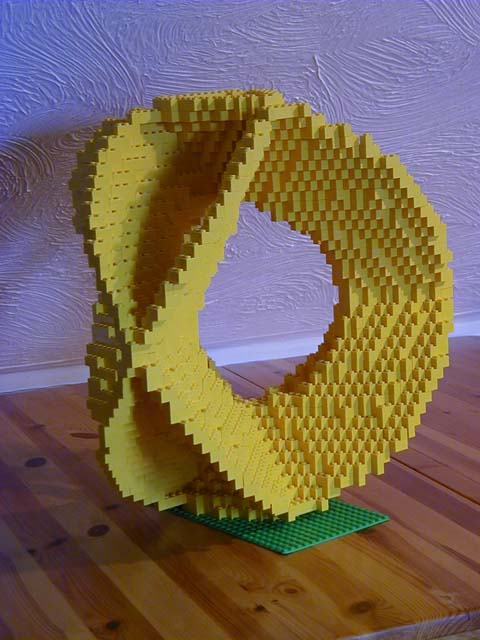
\includegraphics[width=\textwidth]{bours_big.jpg}
%		\caption{Lego Bour's Surface: By Andrew Lipson}
%	\end{figure}
%\end{column}
%\begin{column}{.7\textwidth}
%Thank you!  \\
%Code available at: \\
%\url{http://github.com/appliedtopology/ctl}  \\
%\vspace{1cm}
%Lego Art from: \\ 
%\url{http://andrewlipson.com}
%\end{column}
%\end{columns}
%\end{frame}
\end{document}
